%%%%%%%%%%%%%%%%%%%%%%%%%%%%%%%%%%%%%%%%%%%%%%%%%%%%%%%%%%%%%%%
%% OXFORD THESIS TEMPLATE

% Use this template to produce a standard thesis that meets the Oxford University requirements for DPhil submission
%
% Originally by Keith A. Gillow (gillow@maths.ox.ac.uk), 1997
% Modified by Sam Evans (sam@samuelevansresearch.org), 2007
% Modified by John McManigle (john@oxfordechoes.com), 2015
%
% This version Copyright (c) 2015-2023 John McManigle
%
% Broad permissions are granted to use, modify, and distribute this software
% as specified in the MIT License included in this distribution's LICENSE file.
%

% I've (John) tried to comment this file extensively, so read through it to see how to use the various options.  Remember
% that in LaTeX, any line starting with a % is NOT executed.  Several places below, you have a choice of which line to use
% out of multiple options (eg draft vs final, for PDF vs for binding, etc.)  When you pick one, add a % to the beginning of
% the lines you don't want.


%%%%% CHOOSE PAGE LAYOUT
% The most common choices should be below.  You can also do other things, like replacing "a4paper" with "letterpaper", etc.

% This one will format for two-sided binding (ie left and right pages have mirror margins; blank pages inserted where needed):
\documentclass[a4paper,twoside]{ociamthesis}
% This one will format for one-sided binding (ie left margin > right margin; no extra blank pages):
%\documentclass[a4paper]{ociamthesis}
% This one will format for PDF output (ie equal margins, no extra blank pages):
%\documentclass[a4paper,nobind]{ociamthesis} 

%%%%% SELECT YOUR DRAFT OPTIONS
% Three options going on here; use in any combination.  But remember to turn the first two off before
% generating a PDF to send to the printer!

% This adds a "DRAFT" footer to every normal page.  (The first page of each chapter is not a "normal" page.)
\fancyfoot[C]{\emph{DRAFT Printed on \today}}  

% This highlights (in blue) corrections marked with (for words) \mccorrect{blah} or (for whole
% paragraphs) \begin{mccorrection} . . . \end{mccorrection}.  This can be useful for sending a PDF of
% your corrected thesis to your examiners for review.  Turn it off, and the blue disappears.
\correctionstrue


%%%%% BIBLIOGRAPHY SETUP
% Note that your bibliography will require some tweaking depending on your department, preferred format, etc.
% The options included below are just very basic "sciencey" and "humanitiesey" options to get started.
% If you've not used LaTeX before, I recommend reading a little about biblatex/biber and getting started with it.
% If you're already a LaTeX pro and are used to natbib or something, modify as necessary.
% Either way, you'll have to choose and configure an appropriate bibliography format...

% The science-type option: numerical in-text citation with references in order of appearance.
\usepackage[style=numeric-comp, sorting=nyt, backend=biber, maxcitenames=2, doi=false, isbn=false]{biblatex}


% \usepackage[style=authoryear, sorting=nyt, backend=biber, maxcitenames=2, useprefix, doi=false, isbn=false]{biblatex}
\newcommand*{\bibtitle}{References}

% This makes the bibliography left-aligned (not 'justified') and slightly smaller font.
\renewcommand*{\bibfont}{\raggedright\small}

% Change this to the name of your .bib file (usually exported from a citation manager like Zotero or EndNote).
\addbibresource{references.bib}


% Uncomment this if you want equation numbers per section (2.3.12), instead of per chapter (2.18):
%\numberwithin{equation}{subsection}


%%%%% INCLUDING PACKAGES

% Useful for including algorithms and pseudocide
\usepackage{algorithm}
\usepackage{algpseudocode}

% Required for inserting images
\usepackage{tabularx} 

% For subfigures; subfig and subfigure are both superceded by subcaption
\usepackage{subcaption}
% \usepackage{subfig}
% \usepackage{subfigure}

\usepackage{amsmath}

% For graphics (and sets path to the figure path)
\usepackage{graphicx}
\graphicspath{{./figures/}}


\usepackage{array}
\usepackage{multirow}

\usepackage{wrapfig}
\usepackage[utf8]{inputenc} % allow utf-8 input
\usepackage[T1]{fontenc}    % use 8-bit T1 fonts
\usepackage{hyperref}       % hyperlinks
\usepackage{url}            % simple URL typesetting
\usepackage{booktabs}       % professional-quality tables
\usepackage{amsfonts}       % blackboard math symbols
\usepackage{nicefrac}       % compact symbols for 1/2, etc
\usepackage{microtype}      % microtypography
\usepackage{xcolor}         % colors

% For the cancelto command
\usepackage[makeroom]{cancel}

% For correct real number formatting
\usepackage{amssymb}

% For theorems in body
\newtheorem{theorem}{Theorem}
\newtheorem{corollary}[theorem]{Corollary}
\newtheorem{proposition}{Proposition}
\newenvironment{proof}[1][Proof]

% \usepackage{dcolumn} % Booktabs column spacing
% \usepackage{etoolbox}
% \usepackage{tikz}
% \usepackage[makeroom]{cancel}
% \usepackage{adjustbox}
% \usepackage{comment}
% \usepackage{longtable}
% \usepackage{geometry}
% \geometry{verbose,tmargin=1in,bmargin=1in,lmargin=1in,rmargin=1in}
% \usepackage{setspace}
% \usepackage{makecell}
% \usepackage{soulpos} % for the command \hl
% \usepackage{ulem}
% \usepackage{eurosym}
% \usepackage{color}
% \usepackage{sectsty}
% \usepackage{palatino}
% \usepackage{caption}
% \usepackage{pdflscape}
% \usepackage{csquotes}
% \usepackage{changepage}
% \usepackage{alphalph}
% \renewcommand*{\thesubfigure}{%
% \alphalph{\value{subfigure}}%
% }%

%%%%% THESIS / TITLE PAGE INFORMATION
% Everybody needs to complete the following:
\title{Selection-Oriented AI: The Role of HCI in Supporting Solutions to Explai
nability, Diversity, and Plagiarism in Global Scholarship Selection}
\author{Neil Natarajan}
\college{New College}

% Master's candidates who require the alternate title page (with candidate number and word count)
% must also un-comment and complete the following three lines:
%\masterssubmissiontrue
%\candidateno{933516}
%\wordcount{28,815}

% Uncomment the following line if your degree also includes exams (eg most masters):
%\renewcommand{\submittedtext}{Submitted in partial completion of the}
% Your full degree name.  (But remember that DPhils aren't "in" anything.  They're just DPhils.)
\degree{Doctor of Philosophy}
% Term and year of submission, or date if your board requires (eg most masters)
\degreedate{Trinity 2024}


%%%%% YOUR OWN PERSONAL MACROS
% This is a good place to dump your own LaTeX macros as they come up.

% To make text superscripts shortcuts
	\renewcommand{\th}{\textsuperscript{th}} % ex: I won 4\th place
	\newcommand{\nd}{\textsuperscript{nd}}
	\renewcommand{\st}{\textsuperscript{st}}
	\newcommand{\rd}{\textsuperscript{rd}}

%%%%% THE ACTUAL DOCUMENT STARTS HERE
\begin{document}

%%%%% CHOOSE YOUR LINE SPACING HERE
% This is the official option.  Use it for your submission copy and library copy:
\setlength{\textbaselineskip}{22pt plus2pt}
% This is closer spacing (about 1.5-spaced) that you might prefer for your personal copies:
%\setlength{\textbaselineskip}{18pt plus2pt minus1pt}

% You can set the spacing here for the roman-numbered pages (acknowledgements, table of contents, etc.)
\setlength{\frontmatterbaselineskip}{17pt plus1pt minus1pt}

% Leave this line alone; it gets things started for the real document.
\setlength{\baselineskip}{\textbaselineskip}


%%%%% CHOOSE YOUR SECTION NUMBERING DEPTH HERE
% You have two choices.  First, how far down are sections numbered?  (Below that, they're named but
% don't get numbers.)  Second, what level of section appears in the table of contents?  These don't have
% to match: you can have numbered sections that don't show up in the ToC, or unnumbered sections that
% do.  Throughout, 0 = chapter; 1 = section; 2 = subsection; 3 = subsubsection, 4 = paragraph...

% The level that gets a number:
\setcounter{secnumdepth}{3}
% The level that shows up in the ToC:
\setcounter{tocdepth}{3}


%%%%% ABSTRACT SEPARATE
% This is used to create the separate, one-page abstract that you are required to hand into the Exam
% Schools.  You can comment it out to generate a PDF for printing or whatnot.
% \begin{abstractseparate}
% 	In a globalised world, scholarship programs face pressures to select the ``best'' applicants fairly across regions, but current low-tech selection processes struggle to meet this burden. To address this, we studied two global scholarship programs, exploring data-driven Decision Support Tools (DSTs) for selection. One program was interested in utilising existing AI tools wherever possible. We explored using existing post-hoc explainable AI (xAI) tools as DSTs in a variety of contexts and using existing detection software as DSTs to understand generative AI (genAI)'s role in essays. We developed the \emph{Decision Matrix} framework, categorising decisions by \emph{stage} (\emph{in-process} or \emph{ex-post}) and \emph{stakes} (\emph{high} or \emph{low}), and applied it to assess both technologies as DSTs. Both proved ineffective for \emph{in-process} decisions and useful \emph{ex-post}.

To design a DST for \emph{in-process} decision-making, we engaged in participatory design with both programs, focusing on diversity considerations in selection. Six prototypes were created, with practitioners showing eagerness to use them across the \emph{Decision Matrix}. To validate this enthusiasm, we implemented one design as a technology probe and evaluated its impact. The selected cohort's diversity and performance improved, demonstrating the tool's ability to support high-stakes \emph{in-process} decisions.

Our findings highlight the need for data-driven and AI-based DSTs across the \emph{Decision Matrix}. We propose \emph{Selection-Oriented AI}, focused on the pro-social goals of selection. We conclude with a call for AI-driven DSTs that balance practitioners' needs while optimising selection outcomes for social benefit. % Create an abstract.tex file in the 'text' folder for your abstract.
% \end{abstractseparate}


% JEM: Pages are roman numbered from here, though page numbers are invisible until ToC.  This is in
% keeping with most typesetting conventions.
\begin{romanpages}

% JEM: By default, this template uses the traditional Oxford "Belt Crest". Un-comment the following
% line to use the newer, "Blue Square" logo:
% \renewcommand{\crest}{{
\includegraphics[width=4.2cm, height=4.2cm]{figures/newlogo.pdf}}}

% Title page is created here
\maketitle

%%%%% DEDICATION -- If you'd like one, un-comment the following.
%\begin{dedication}
%This thesis is dedicated to\\
%someone\\
%for some special reason\\
%\end{dedication}

%%%%% ACKNOWLEDGEMENTS -- Nothing to do here except comment out if you don't want it.
\begin{acknowledgements}
 	I would like to thank my advisors Reuben Binns and Nigel Shadbolt: Reuben, for his constant dedication to his students and willingness to run with any idea I came up with; Nigel, for his clear framing and pointed critiques. I would also like to thank my colleagues in Oxford Computer Science's HCAI theme, with special thanks to Sruthi, Ulrik, Jake, and Thomas. I would like to thank my family for their support and my friends for my sanity.
\end{acknowledgements}

%%%%% ABSTRACT -- Nothing to do here except comment out if you don't want it.
\begin{abstract}
	In a globalised world, scholarship programs face pressures to select the ``best'' applicants fairly across regions, but current low-tech selection processes struggle to meet this burden. To address this, we studied two global scholarship programs, exploring data-driven Decision Support Tools (DSTs) for selection. One program was interested in utilising existing AI tools wherever possible. We explored using existing post-hoc explainable AI (xAI) tools as DSTs in a variety of contexts and using existing detection software as DSTs to understand generative AI (genAI)'s role in essays. We developed the \emph{Decision Matrix} framework, categorising decisions by \emph{stage} (\emph{in-process} or \emph{ex-post}) and \emph{stakes} (\emph{high} or \emph{low}), and applied it to assess both technologies as DSTs. Both proved ineffective for \emph{in-process} decisions and useful \emph{ex-post}.

To design a DST for \emph{in-process} decision-making, we engaged in participatory design with both programs, focusing on diversity considerations in selection. Six prototypes were created, with practitioners showing eagerness to use them across the \emph{Decision Matrix}. To validate this enthusiasm, we implemented one design as a technology probe and evaluated its impact. The selected cohort's diversity and performance improved, demonstrating the tool's ability to support high-stakes \emph{in-process} decisions.

Our findings highlight the need for data-driven and AI-based DSTs across the \emph{Decision Matrix}. We propose \emph{Selection-Oriented AI}, focused on the pro-social goals of selection. We conclude with a call for AI-driven DSTs that balance practitioners' needs while optimising selection outcomes for social benefit.
\end{abstract}

%%%%% MINI TABLES
% This lays the groundwork for per-chapter, mini tables of contents.  Comment the following line
% (and remove \minitoc from the chapter files) if you don't want this.  Un-comment either of the
% next two lines if you want a per-chapter list of figures or tables.
\dominitoc % include a mini table of contents
%\dominilof  % include a mini list of figures
%\dominilot  % include a mini list of tables

% This aligns the bottom of the text of each page.  It generally makes things look better.
\flushbottom

% This is where the whole-document ToC appears:
\tableofcontents

% Uncomment to generate a list of figures:
% \listoffigures
% 	\mtcaddchapter

% \mtcaddchapter is needed when adding a non-chapter (but chapter-like) entity to avoid confusing minitoc

% Uncomment to generate a list of tables:
%\listoftables
%	\mtcaddchapter

%%%%% LIST OF ABBREVIATIONS
% This example includes a list of abbreviations.  Look at text/abbreviations.tex to see how that file is
% formatted.  The template can handle any kind of list though, so this might be a good place for a
% glossary, etc.
% First parameter can be changed eg to "Glossary" or something.
% Second parameter is the max length of bold terms.
\begin{mclistof}{List of Abbreviations}{3.2cm}
    \item[AI] Artificial Intelligence
    \item[xAI] Explainable Artificial Intelligence
    \item[DEI] Diversity, Equity, and Inclusion.
    \item[IAI] Interpretable Artificial Intelligence
    \item[DST] Decision Support Tool
    \item[HitL] Human in the Loop 
    \item[IAIDST] Interpretable, Artificially Intelligent Decision Support Tool
    \item[TI] Talent Identification 
\end{mclistof}
See Appendix \ref{app:terminology} for definitions of terms used in this Thesis, including these abbreviations.

% The Roman pages, like the Roman Empire, must come to its inevitable close.
\end{romanpages}


%%%%% CHAPTERS
% Add or remove any chapters you'd like here, by file name (excluding '.tex'):
\flushbottom
% \begin{savequote}[8cm]
% \textlatin{Neque porro quisquam est qui dolorem ipsum quia dolor sit amet, consectetur, adipisci velit...}

% There is no one who loves pain itself, who seeks after it and wants to have it, simply because it is pain...
%   \qauthor{--- Cicero's \textit{de Finibus Bonorum et Malorum}}
% \end{savequote}

\chapter{\label{ch:intro}Introduction} 

\minitoc

% To-do: rewrite

Since early theorising about Artificial Intelligence (AI), experts have noted the transformative potential of such technology. Now, with the popular advent of Machine Learning (ML) models and transformer architecture in particular, we see rapid mass-market adoption of a variety of AI tools. In many fields which deal with sensitive decision-making, this adoption introduces new ethical challenges. In the fields of talent and Talent Identification (TI) in particular, many of these ethical challenges centre on decision tool interpretability; diversity, equity, and inclusion (DEI); and applicant usage of generative AI. In this section, we lay out the case for the application of AI systems (specifically interpretable AI decision assistants) to these issues in TI, paying special attention to the potential pitfalls and broader implications of our proposal.

\section{Abstracts from Papers} %to-do: replace this with something more coherent.

\subsection{GenAI}
Applicants increasingly use generative AI (genAI) to write essays for universities, jobs, and scholarships. While genAI detectors serve as anti-plagiarism tools, these detectors don’t fully address the challenges faced by selection. Through Action Research (AR) with scholarship selection practitioners, we identified key decisions surrounding genAI, (e.g., whether and how to ban their use in application or broader revisions to application processes). We developed a framework for categorising these decisions and assessed two popular detectors, Originality.ai and GPTZero. Although neither detector fully meets the needs for reliably identifying and disqualifying AI-plagiarised essays, both can support ex-post process decisions. We applied GPTZero to evaluate genAI use across years and by channel partners (who source and support program applicants), finding an overall increase in genAI usage year-over-year but no evidence of widespread genAI use among channel partners. Our findings support the program’s channel partnership approach but suggest the need for new assessment methodologies.

\subsection{XAI}
Post-hoc Explainable AI (xAI) methods build trust in AI-based Decision Support Tools (DSTs), but critics warn they may induce decision-maker over-reliance on AI. We differentiate between two decision stages for using xAI: \emph{in-process}, where xAI informs primary decisions (e.g., whether to select a candidate), and \emph{ex-post}, where xAI informs second-order decisions (e.g., whether to change the candidate selection process). In an online study, we evaluate three xAI methods (SHAP, Anchor, and Confidence) \emph{in-process} and find that SHAP and Confidence induce unwarranted trust. We then conduct participatory design sessions presenting SHAP explanations to scholarship selection practitioners in the \emph{ex-post} context. These explanations can inform and support \emph{ex-post} decisions, but effective presentation and contextualisation is key. We conclude that, while critics’ warnings of xAI-induced misplaced trust hold \emph{in-process}, this misplaced trust is not unique to post-hoc xAI. Furthermore, post-hoc xAI methods, even if misleading \emph{in-process}, can still be valuable \emph{ex-post}.

\subsection{Diversity}
When selecting applicants for scholarships, universities, or jobs, practitioners often aim for a diverse cohort of qualified recipients. However, differing articulations, constructs, and notions of diversity prevents decision-makers from operationalising and progressing towards the diversity they all agree is needed . To understand this challenge of translation from values, to requirements, to decision support tools (DSTs), we conducted participatory design studies exploring professionals' varied perceptions of diversity and how to build for them. Our results suggest three definitions of diversity: bringing together \emph{different perspectives}; \emph{ensuring representativeness} of a base population; and \emph{contextualising applications}, which we use to create the \emph{Diversity Triangle}. We experience-prototyped DSTs reflecting each angle of the \emph{Diversity Triangle} to enhance decision-making around diversity. We find that notions of diversity are highly diverse; efforts to design DSTs for diversity should start by working with organisations to distil `diversity' into definitions and design requirements.

\subsection{SPF}
We hypothesize that the complexity of selecting personnel in a way that jointly optimizes for talent (performance on an ability measure) and diversity impedes organizations from meeting their diversity, equity, and inclusion goals. To formalize this, we prove that maximizing cohort diversity is computationally complex and incorporate this complexity into a selection model by adding computational costs. To test the model's predictions, we construct an algorithm to estimate the diversity-talent frontier, which we apply to data from a scholarship and talent investment program. We find that finalists could have been 13\% (15.6\%) more diverse (more talented) without reducing talent (diversity). We also show that the program selected a significantly more diverse and talented cohort after we provided them with a frontier estimate. We conclude by using program data to demonstrate how the frontier estimation procedure can be used to evaluate the efficacy of alternative screening approaches. This reveals that if the program had screened on IQ, they would have significantly reduced diversity and overlooked many of the most talented applicants.

\section{Motivation}
(To-do) This is where I explain why I'm doing this research. I explain why care about talent identification and how IAIDSTs can solve problems here. I respond to the notion that we should simply not use AI here, and highlight problems in the field already. I explain why this is a problem for Computer Science as well as for Talent Science (tl;dr: additional reasons to care about things xai overlooks because of the application domain)

\section{Contributions}
In this thesis, we make a number of theoretical, technical and practical contributions. These are:

\begin{itemize}
    \item We articulate where talent identification experts should use IAIDSTs to assist in their decision-making, and which IAI systems are appropriate for which purposes
    \item We apply research-through-design methods to talent identification to produce a novel approach to the creation of human-centric selection tooling
    \item We develop a novel method for visualising and understanding cohort-level decisions surrounding diversity called the Selection Possibility Frontier
    \item We further implement a novel algorithm for approximating the Selection Possibility Frontier
    \item We produce several qualitative, quantitative, and mixed-modal datasets relating to talent identification
    \item We demonstrate a yet-undemonstrated risk associated with naive application of post-hoc explainability to a range of problems
    \item We demonstrate the utility and limitation of detection tools for generative-AI-written essays in a scholarship context, and explore implications for scholarship programs
\end{itemize}

\section{Thesis Structure}
In this chapter, we explore our motivation for focusing on the application of IAIDSTs to talent identification, enumerate our contributions, and provide an account of challenges talent identification. Among these challenges, we focus the remainder of this thesis on three: limited human understanding of the AI tools, limited ability to consider diversity, and the risks of applicant usage of generative AI.

In Chapter \ref{ch:background}, we provide a background on the field of talent identification, the field of explainable AI, and the field of diversity, equity, and inclusion; we further explore intersections between these fields of research and identify gaps in the literature. Chapters \ref{ch:xailimitations} and \ref{ch:usingxai} explore our first challenge: limited human understanding of the AI tools. In Chapter \ref{ch:xailimitations}, we explore the limitations of popular xAI methods in the context of talent identification. In Chapter \ref{ch:usingxai}, we explore the use of SHAP explanations in the context of talent identification. Chapters \ref{ch:iaicasestudy} and \ref{ch:spf}  address challenges related to consideration of diversity in TI. In Chapter \ref{ch:iaicasestudy}, we present a participatory design study, which aims to use IAIDSTs to help TI professionals account for diversity. In Chapter \ref{ch:spf} we implement one of the designs from Chapter \ref{ch:iaicasestudy}. Chapter \ref{ch:studentuse} attempts to mitigate the risks of applicant usage of generative AI. It explores the use of generative AI detection tools as DSTs in the context of talent identification. Finally, in Chapter \ref{ch:discussion}, we discuss our design recommendations, note limitations of our approach, and conclude.

\section{Publications}

\begin{itemize}
    \item \textcite{natarajan_trust_2023} Trust Explanations to do What They Say
    \item \textcite{citation needed} `You Trust Me, But Should You?': Misleading Explanations of AI Outputs
\end{itemize}
% \begin{savequote}[8cm]
% \textlatin{Neque porro quisquam est qui dolorem ipsum quia dolor sit amet, consectetur, adipisci velit...}

% There is no one who loves pain itself, who seeks after it and wants to have it, simply because it is pain...
%   \qauthor{--- Cicero's \textit{de Finibus Bonorum et Malorum}}
% \end{savequote}


\chapter{\label{ch:rw}Related Works} 
\minitoc

\section{Decision Support Tools for Scholarship Selection}

% to-do

\section{Explainable Artificial Intelligence}
% to-do: rewrite
\subsection{Types of Explainable Artificial Intelligence Publications}

The field of explainable Artificial Intelligence (xAI) can, broadly, be divided into four main bodies of research: reviews, methods, notions, and evaluations \cite{vilone_explainable_2020}. Review articles are either systematic investigations or literature reviews. Method articles introduce new explanation methods. Notion articles focus on defining notions or concepts related to explainability. Evaluation articles evaluate existing notions or paradigms.

\subsubsection{Review Articles}
Review articles offer meta-commentary on other articles listed below. A review article is so-characterised because its primary contribution is one of aggregation. Thus, a review article might also be a method, notion, or evaluation article, so long as it primarily draws from these articles. This paper is, primarily, a review article.

\subsubsection{Method Articles}
In most method articles, the task of explanation is taken to be fairly well-defined, and the research questions deal in how to most effectively generate that explanation. 

Consider two particular method articles: SHAP explanations, introduced by \textcite{lundberg_unified_2017}, and counterfactual explanations, introduced by \textcite{wachter_counterfactual_2017}. In both papers, we see heavy treatment of the mathematical properties of the explanation algorithm introduced. However, we see relatively light treatment of what the authors take to be a good explanation or proposed use cases for the novel methods. These concepts are instead the domain of notion articles.

\subsubsection{Notion Articles}
Where method articles deal with individual methods, notion articles deal with theory underlying a variety of methods. For example, \textcite{miller_explanation_2017} discussion of the importance of principles of explanation from the social sciences is a notion article.

\subsubsection{Evaluation Articles}
Evaluation articles consider which notions and methods are best-suited to produce the best explanations. Evaluations of method articles, in particular, often compare them to notions introduced elsewhere, and where critiques are found, they are often critiques that the method fails to meet a standard set by the notion.

For the two method articles discussed above, we present two evaluation articles: \textcite{kumar_problems_2020} evaluation of the SHAP method, and \textcite{barocas_hidden_2020} evaluation of counterfactual explanations. Both articles rely on similar notions regarding the purpose of explanations, and critique the methods for failing to adhere to a notion. For instance, \textcite{barocas_hidden_2020} assume that counterfactual explanations are given to provide users actionable information. Similarly, \textcite{kumar_problems_2020} argue that SHAP cannot be used to inform users' actions.

\subsection{A Taxonomy of XAI Methods}
AI model explanations can broadly be categorised into two subgroups: intrinsically interpretable models and post-hoc explanations \cite{molnar_interpretable_2019}. Though intrinsically interpretable models are often not classed as ``xAI'' (as they do not make use of developments in xAI), they do offer offer explanations \cite{molnar_interpretable_2019}, since they are already interpretable; thus, we include them here.

Post-hoc methods can be further separated into global methods, which explain entire models, and local methods, which explain individual decisions \cite{molnar_interpretable_2019}. When assessing explanation methods, one can distinguish between local tests and global tests of model explanations \cite{molnar_interpretable_2019}. Local tests concentrate on the impact of the explanations at the level of a single prediction, global tests focus on the impact of explanations on overall model trust.

Rather than delineating between intrinsic and post-hoc or global and local, we could instead delineate by output type \cite{friedrich_taxonomy_2011}. Some interpretability devices offer feature importance statistics. Others offer explanations by contrast to another datapoint. Yet others offer rules that guide decision-making in regard to an individual case case.

\subsection{Use Case}
Consider the following potential use cases for xAI methods: to evaluate whether the AI is operating as intended, to examine an AI for bias and unfairness, to provide recourse, to provide a rule that would guarantee equality. This list is not exhaustive, and yet, even for these three use cases, explanations that satisfy some will not satisfy others \cite{natarajan_trust_2023}.

\subsection{Theories of Explanation}
In deciding which type of explanation will best suit a particular use case, we must consider the theory of explanation that underlies the explanation, and the desiderata that that theory demands of its explanations.

\textcite{miller_explanation_2017} summarises key findings from Social Sciences related to explanation. \textcite{miller_explanation_2017} works from a causal theory of explanation; he outlines and examines the theory, noting challenges to it, but does not consider a rejection of the theory. According to the theory, explanations are sought in response to counterfactual cases, i.e. the question asked is not of the form "Why \textit{P}" but rather "Why \textit{P} instead of \textit{Q}" \cite{miller_explanation_2017}. Such counterfactual theories of causality all argue that cause is a matter of what would have happened if the cause had not happened. Though they disagree on precisely how to model these counterfactual cases, many leading philosophical theories of causality agree that causality is best understood in terms of counterfactuals. Hume modeled these counterfactuals in terms of causes and events: in actuality, cause $C$ caused event $E$ to occur; but if cause $C'$ had replaced cause $C$, $E$ would not have occurred. We can call this sort of counterfactual a cause-counterfactual \cite{miller_explanation_2017}. Under this conception, explanations should present cause-counterfactuals as clearly as possible.

\textcite{miller_explanation_2017} also argues that explanations should be contrastive and selective. Contrastive explanations make use of counterfactuals, but these counterfactuals are not cause-counterfactuals. Instead, they are event-counterfactuals. In other words, contrastive explanations consider alternative events $E'$, and explain the data $E$ in relation to $E'$. Selective explanations, on the other hand, are ones that do not consist of a complete cause, but rather select one or two causes from the complete cause. 

\textcite{miller_explanation_2017} presents a powerful application of a theory of explanation to the field of xAI. However, causal theories of explanation are far from the only type of explanatory theories. Indeed, as we noted above with numerical evidence, there are theories of explanation who's desiderata contradict those of \textcite{miller_explanation_2017}'s causal theory \cite{woodward_scientific_2021}. 

In what follows, I present \textcite{woodward_scientific_2021}'s theory, the statistical relevance model of explanation. The statistical relevance theory rests heavily on the notion of statistical relevance. For events $A$, $B$, and $C$, we say $C$ is statistically relevant to $B$ in $A$ if and only if $P(B | A \land C) \neq P(B | A)$. I.e., an explanation is a member $C_i$ of a homogeneous partition $C$ of properties: that is, a set of properties that are exclusive and exhaustive of $A$, where there are no statistically relevant properties $D$ to $B$ in $A \land C_i$. The explanation also consists of $P(B | A)$, the probability $P(B | A \land C_i)$ of each cell withing the partition, and which of the $C_i$ contains the desired point to be explained, $x$ \cite{woodward_scientific_2021}.

On both accounts , explanations have an explainer and an explainee. Explanations in everyday use are an interaction. Unlike most modern algorithmic explanation methods, an explanation given by a human is often given in the form of a conversation. Thus, it obeys the rules of communication using language. In other words, these explanations are social. We may therefore apply theories governing social interactions, such as \textcite{Grice_1975}'s conversational maxims, to explanations \cite{miller_explanation_2017}.

\textcite{Grice_1975}'s four categories of conversational maxims are: quality, quantity, relation, and manner. That is, the quality of information conveyed in a cooperative conversation should be high (information should be likely and justifiable). The quantity of information should be neither too little nor too much. The information should be related to the conversation. The information should be conveyed in an appropriate manner. Note that the quantity bounds overlap quite heavily with selectivity.

\subsection{Trust}
Another important notion related to xAI is trust. Indeed, much of the xAI literature suggests that the purpose of xAI is to increase trust in AI. This is apparent from the titles of canonical papers in the field, such as \textcite{ribeiro_why_2016} and \textcite{pieters_explanation_2011}. So what does it mean to trust an AI system? A basic philosophical analysis of what trust consists in (in the general, non-algorithmic sense) is as follows: $A$ trusts $B$ if and only if $A$ believes that $B$ will act in $A$'s best interest, and $A$ accepts vulnerability to $B$'s actions \cite{jacovi_formalizing_2021}. Moreover, trust often does not have a blanket scope; typically, $A$ will trust $B$ regarding some particular actions or motivations.

An important distinction here can be drawn between whether someone or something is trusted and whether that trust is warranted; i.e. it is worthy of trust \cite{hardin_trust_2002}. In the context of AI, according to \textcite{jacovi_formalizing_2021}, we should only ever trust AI systems to fulfil their contracts, but some AI systems are not worthy of even this trust. Ideally, trust in a system should relate directly to that system's trustworthiness – we should place trust in any system when it warrants trust, but should not place unwarranted trust in any system. The problem of appropriately calibrating trust, however, is yet unsolved.

There are many methods that aim to calibrate trust in an AI algorithm. We could give some access to the patterns that distinguish correct and incorrect cases. The better some end-user is able to distinguish these, the better they know when they can trust the model to be correct. Knowledge of the performance of a model grants access to the patterns distinguishing correct and incorrect cases. Facts about the bias of the model grant access as well, as does information about the performance of the model on a subset of data. Explanations can be seen as one way of imparting such information. Because of this, algorithm explanations allow explainees to determine when an algorithm is trustworthy. 

\subsection{Relevant Evaluations of XAI}
There is a growing body of studies that empirically evaluate xAI methods. In some cases, an xAI method is evaluated not with human subject experiments but rather with some formally defined proxy for interpretability \cite{doshi-velez_towards_2017}. However, most evaluations involve humans using an AI system to perform some task, and the effect of an xAI method on task performance is measured.  For our purposes, namely the measurement of end-user trust and reliance, we need to measure lay people using a system in a simplified but realistic task.

It should also be noted that there is no standard evaluation or set of benchmarks explainability methods are judged by \cite{doshi-velez_towards_2017}. Indeed, though there are proposed methods for evaluating attribution-based explanations and model-based explanations, there are none for evaluating example-based explanations \cite{markus_role_2021}. As a result, there exist a variety of study designs, conditions, and variables measured by human-centred evaluation papers. We list some such studies here.

\textcite{ford_play_2020} run a study where they examine the impact of post-hoc explanations-by-example and error-rates on people's perceptions of a black-box classifier. They show that case-based explanations lead participants to perceive miss-classifications as more correct. In the case of their study, a case-based explanation is a series of three important data points in the training of the model (in other words, an “influential instances” explanation). They also show that classifiers with higher error rates lead participants to perceive the models as less trustworthy. They show participants a series of machine classifications of the MNIST dataset, where the model either correctly labels the data or commits an alternate labelling error. They then task the participants with rating correctness and reasonableness of each classification on a 5-point scale. Finally, at the end, the participants filled out global correctness and reasonableness, alongside global trust forms. The design was a 2x3 design, with explanations present or absent, and three accuracy levels. Participants report miss-classifications as being more correct when given a case-based explanation. They did not find significant findings for reasonableness, trust, or satisfaction across explanation-present or explanation-absent conditions. They use a MANOVA design to account for differences across conditions, but use a between-subjects design \cite{ford_play_2020}. 

\textcite{jacobs_how_2021} run a study in the medical diagnosis context, where participants are given a vignette of a patient and, in the experiment condition, a recommended treatment list and explanation. Participants were asked to make an antidepressant treatment selection, to rate their confidence, and to indicate the utility of the model on their decision (it appears on a 5-point scale). The study had statistically significant results only with respect to accuracy (measured as an average of 0s and 1s), not confidence or perceived utility. In the accuracy case, this indicated that an algorithmically generated treatment list, when wrong, would mislead the participants and lower their accuracy. In the confidence and utility cases, this would indicate either that accuracy is affected, but not confidence or utility, or that the Likert scale measurement method used in Jacobs et al.'s study is a weaker measurement tool than the accuracy. Furthermore, these findings are not isolated to the explanation. Rather, Jacobs et al. consider the recommendation and the explanation together. For example, they find that feature-based explanations, paired with incorrect recommendations, lowered accuracy compared to the baseline condition (no recommendation) \cite{jacobs_how_2021}. 

\textcite{bansal_does_2021} perform another similar study, looking at human-AI cooperation in a context where they have comparable performance. They use sentiment classification as their task. Furthermore, they measure effects with a variety of explanations. They find that explanations inspire increased trust in AI systems regardless of the correctness of the model. As explanation, they use a highlighting of the top predicted sentiment classes, alongside a highlighting of important words. Finally, they test expert-generated explanations to serve as an upper bound, as they found that humans were often confused when machine explanations made little sense. They note that explanations make the user more likely to have high accuracy when the AI is correct, but more likely to have low accuracy when the AI is incorrect. This would indicate that AI recommendations with explanations are capable of fostering mistrust, as they foster both overtrust and under trust \cite{bansal_does_2021}.

\textcite{mohseni_trust_nodate} measure user trust in an AI fake news detection system over time. They design a study in which users are shown true and fake news articles. The users are asked at three different points (each one additional third through the study) what their perceived accuracy of the explainable AI system is. They had three different conditions, segmented by type of explanation. There was a baseline condition with no explanation and two xAI conditions. They show that the user trust can be clustered into five profiles: consistent overtrust, consistent under trust, consistent trust, trust gains continually, and trust decreases continually. They show that more participants from the no explanation and attribute explanation conditions were consistently gaining trust, and that more participants from the attention explanation condition overshot their second perceived accuracy measurement \cite{mohseni_trust_nodate}.

\section{Generative AI Detectors}
% to-do

\section{Approaches to Considerations of Diversity}
% to-do
% \begin{savequote}[8cm]
% \textlatin{Neque porro quisquam est qui dolorem ipsum quia dolor sit amet, consectetur, adipisci velit...}

% There is no one who loves pain itself, who seeks after it and wants to have it, simply because it is pain...
%   \qauthor{--- Cicero's \textit{de Finibus Bonorum et Malorum}}
% \end{savequote}

\chapter{\label{ch:methods}Methodology}

\minitoc

\section{Paradigms}
\subsection{Participatory Design}\label{ssec:participatory_design}
Participatory Design (PD) is a design paradigm in HCI emphasising active involvement of all stakeholders, particularly end-users, in the design process \cite{Hussain2014OverviewOV}. This approach recognises these users as best-positioned to speak to their subjective needs and preferences \cite{Hussain2014OverviewOV}, ensuring that designs meet user needs.

PD is a fundamentally collaborative process in which the designers and users work together to create solutions \cite{Tokranova2022ApplyingPD}. By involving users in each iteration of the development of a design, PD empowers participants to build tools that serve them \cite{Hussain2014OverviewOV}.

Historically, PD has placed special emphasis on inclusion of a broad variety of user groups \cite{Brankaert2019IntersectionsIH}. For example, \textcite{10.1145/3544549.3573821,10.1145/3544548.3580933,Chowdhury2023ReflectionsOO} employ child-centric PD. \textcite{Brankaert2019IntersectionsIH} call for (and employ) PD aiming to serve users with dementia.

This focus on inclusion, especially a focus on inclusion of oft-overlooked groups, is in itself a value-laden assumption of the PD process. That is, to employ PD is to assert the voices of the selected participants as valuable, both in the design of the tool and in the broader context of research.

\subsection{Action Research}\label{ssec:action_research}\footnote{This section reproduces text from Chapter \ref{ch:genai}.}
Action Research (AR) is a research philosophy that emphasises ``research with, rather than on, people'' \cite{bradbury_action_2003}. Rather than one specific method, AR is best seen as a collection of related methods all embodying this ethos, usually with the goal of producing research contributions useful to the target group of people \cite{lu_organizing_2023}. Among these are semiotic inspection \cite{DeSouza_Leitão_2009,Alvarado_Waern_2018} and participatory design  (PD) \cite{braun_using_2006,Griffiths_Johnson_Hartley_2007,blythe2014research,Knapp_Zeratzky_Kowitz_2016}. AR is most often used in the context of social work, but can be applied across a variety of fields \cite{dombrowski_social_2016,lu_organizing_2023}. 

In education, AR is often used in a classroom setting \cite{Mertler_2019}. \textcite{venn-wycherley_realities_2024} argue that it is crucial in this setting to perform AR on both educators (teachers) and educatees (students), as failing to do so is liable to yield contributions useful to one group but not the other. While this holds for classroom settings, engagement across the stakeholder map is less feasible or desirable in scholarship selection. Unlike teacher and student, who share the common goal that the student learn, selector and applicant are at cross purposes: practitioners seek to choose the `best' cohort of applicants (although they often disagree on what constitutes `best'), while applicants seek to be included in the chosen cohort \cite{bergman2021seven}. Thus, when elucidating the interests and desires of one group, the other will merely act as noise. (E.g., applicants who use genAI to assist in writing their application will, of course, oppose using systems that monitor genAI usage to disqualify applicants.)

AR is comparatively new to HCI \cite{Hayes_2011,lu_organizing_2023}, but its methods and philosophies closely mirror longstanding pillars of HCI \cite{Hayes_2011}. Much like PD and other HCI methods, AR seeks to democratise the research and design processes; unlike PD, AR extends beyond building solutions democratically, and sees learning through action as the ultimate research contribution \cite{Hayes_2011}. For example, AR sees all parties Become: ``Co-investigators of, co-participants in, and co-subjects of...the project'' \cite{Hayes_2011}.  Thus, research questions are formulated by and with participants, actions and interventions are designed by and with participants, and results are found by and with participants \cite{Hayes_2011}.

\subsection{The Relationship between PD and AR}
While PD and AR share the notion that research participants should be closely involved in the research process, they differ in their ontology.

The two differ in the nature of their research outputs. PD is primarily concerned with the design process of products, systems, or interfaces; thus, research contributions are primarily those finalised designs \cite{zimmerman_research_2014}. AR, in contrast, is primarily concerned with the learning that occurs through action; contributions in AR are more often learnings that occurred in the act of doing \cite{Hult1980TOWARDSAD}. 

They also differ in the kinds of research. While PD employs an iterative design process (and often involves evaluation), each stage in this iteration is a design stage. AR, in contrast, involves cycles of three distinct activities: planning (i.e., design), acting, and reflecting \cite{Hult1980TOWARDSAD}.

Finally, and most importantly, they differ in the relative role of the user. In PD, the user \emph{participates} in the act of design; a distinction remains between researchers, who facilitate discussion and implement user requirements, and participants, who discuss and require \cite{Hussain2014OverviewOV}. In AR, this distinction is elided, rendering the participant a co-researcher; it is not uncommon for participants to appear as authors in AR processes \cite{Hayes_2011}. In PD, the user is involved in the design process, while in AR, the user is involved in the research process.

\section{Methods} % To-do: add in these methods.
\subsection{Online Surveys}
The practice of running online surveys to gather quantitative data is well-established and often used both within and without HCI \cite{zhao2023fairness,pillai_adoption_2020,krishna_disagreement_2022,mai_user_nodate,bansal_does_2021,binns_its_2018,dzindolet_role_2003,papenmeier_its_2022}. Chapter \ref{ch:xai} makes use of one such survey. As is standard, we use Prolific Academic to gather participants and Formr to administer our survey \cite{binns_its_2018,Arslan_formr_2019}. More interestingly, we follow \textcite{caldwell_power_nodate} in designing our survey based on a power analysis of the statistical tests we intend to run on the output data. This power analysis, as well as our hypotheses, can be found in our preregistration \cite{natarajan_binns_2022}.

\subsection{Design Workshops}
Chapters \ref{ch:xai} and \ref{ch:diversity} both make use of group design workshops to refine and evaluate design prototypes. Both follow an experience-prototype methodology \cite{Buchenau_Suri_2000}, and incorporate a few specific methodologies.

Both chapters follow \textcite{Zimmerman_Forlizzi_2017}'s scenario speed dating approach, which sees participants rapidly applying different design prototypes to (real or hypothetical) scenarios.

\textcite{Gatian_1994} has researchers asking participants to choose a favourite among a series of options as a means of comparison, while \textcite{Griffiths_Johnson_Hartley_2007} brings this method to HCI. Chapter \ref{ch:diversity} makes use of this method.

\subsection{Individual Interviews}
Chapter \ref{ch:diversity} makes use of one-on-one interviews with participants to first elucidate participant understanding of diversity. In these interviews, we incorporate a number of methods.

\textcite{Knapp_Zeratzky_Kowitz_2016}'s `crazy 8s' exercise sees participants give eight feature requests in eight minutes. Ordinarily, this exercise is done with a writing surface, but we have participants do this verbally.

\textcite{blythe2014research} introduces the concept design fiction, where participants more detail their ideal app. We adapt this to create a ``magic app'', capable of doing anything the participant desires, and asking the participant to describe this app.

\subsection{Quantitative Analysis}
Chapters \ref{ch:xai}, \ref{ch:genai}, and \ref{ch:spf} rely on a number of standard statistical tests. Primarily, we use Student's t test \cite{Mishra_Singh_Pandey_Mishra_Pandey_2019}, the Analysis of Variance (ANOVA) \cite{Mishra_Singh_Pandey_Mishra_Pandey_2019}, Pearson's test of correlation \cite{Schober_Boer_Schwarte_2018}, Tukey's Honestly Significant Difference test \cite{Kim_2015}, and the Reciever Operating Characteristic curve \cite{hanley1989receiver}. Additionally, we develop our own permutation test in Chapter \ref{ch:spf} based on \textcite{good2013permutation}.

\subsection{Qualitative Analysis}
Chapters \ref{ch:xai} and \ref{ch:diversity} engage in inductive thematic analyses of their qualitative results. In doing so, we follow the methodology introduced by \textcite{braun_using_2006} and developed in \textcite{braun_conceptual_2022,braun_toward_2023,noauthor_thematic_nodate}.
\chapter{\label{ch:context}Decisions in the Global Talent Selection Context}
\minitoc

\section{The Social Value of Selection}\label{sec:social_value}
Scholarship programs offer long-term benefits to their chosen scholars, often under the theory that providing these benefits improves not only the welfare of the scholars themselves but of society as a whole \cite{DilraboJonbekova_Ruby_2023,Dassin_Marsh_Mawer_2018}. Theories of the mechanisms of this social benefit vary. Some theories rely on the future actions of the chosen scholars. For example, \textcite{Dassin_Marsh_Mawer_2018} argue that scholars are often empowered and disposed to devote themselves to solving global problems. \textcite{Dassin_Marsh_Mawer_2018} also note that these scholars may bring additional returns to their communities, thereby improving the welfare of a broad group of people (though they also express concern over `brain drain', where these scholars do not return to their communities). In contrast, others contend that the mere provision of scholarships to the correct recipients is itself pro-social. \textcite{minkin2023diversity} note that society benefits from making space for a breadth of perspectives; providing scholarships to those who would otherwise be unable to afford higher education may create that breadth of perspectives. Some evidence suggests that this broader range of perspectives brings additional benefits in the form of increased productivity \cite{autor2008does,noray2023systemic}. Besides the gain to organisations, though, some argue that the social mobility brought about by the existence of scholarship programs yields inherent benefit to society \cite{Dassin_Marsh_Mawer_2018}. Under any of these theories, selecting the ``best'' applicants as scholars is clearly in society's best interest. However, as we explore throughout this thesis, different theories of change yield different definitions of ``best''.

Traditional selection is a human-led process, and many suggest it should remain that way \cite{Latzer_Hollnbuchner_Just_Saurwein_2014}. However, as the number of applicants to scholarship programs grows, the need for scalable selection processes has grown; with traditional selection processes unequipped to handle these new challenges, organisations are forced to innovate, often turning to algorithmic solutions that offer to solve these difficult problems \cite{Latzer_Hollnbuchner_Just_Saurwein_2014}. This has led to the development of Decision Support Tools (DSTs) to support selection processes. These DSTs range from simple tools like automated essay scoring to more complex tools like AI-driven selection algorithms. The use of these tools is not without controversy. Critics argue that these tools may be biased \cite{dwork_fairness_2012}, or may dehumanise the selection process \cite{binns_its_2018}. However, while certain features of these tools may succumb to some critiques, evolving discussions about fairness in selection render older, human-led selection processes equally vulnerable to critique \cite{Ahnaf2023AHPAP,pmlr-v80-kearns18a}.

\section{Related Work}
This thesis engages primarily with literature seeking to use AI tools to support decision-making in global scholarship selection processes. Unfortunately (or perhaps fortunately), this particular niche of literature is fairly sparse. While many tools do exist, especially those seeking to automate the job of the scholarship selector entirely, we are forced to look beyond this niche for a larger body of related literature. Primarily, we do this by considering other selection contexts (e.g., universities or recruiters). Note that while this body of literature is large, and contains work ranging from automated essay scoring to intellect testing \cite{cozma_automated_2018,condon2014international}, our work is only tangentially related to these fields. Some work explores applicant perceptions of scholarship selection processes \textcite{10.1145/3351095.3372867}, but this work is primarily interested in the decision subjects and does not engage with the design of selection processes.

More closely related is the body of algorithmic fairness literature engaging with recruitment, much of which seeks to ensure that AI tools do not discriminate against protected classes \cite{dwork_fairness_2012}. However, as we explore in this chapter, disanalogies between recruitment and global scholarship selection limit the applicability of this work.

Similarly, much work explores the impact of algorithms on educational outcomes. For example, \textcite{NISSENBAUM1998237} explore the risk of algorithmic involvement in education dehumanising the experience. However, though these works are conducted in the same environment, they do not touch on selection itself.

This chapter also explores a model of selection as subordinate decisions and investigations supporting the ultimate decision about which subset of applicants to select as scholars. Many of these subordinate decisions relate to their own bodies of literature; these are explored in the relevant chapters.

\section{On Working with Scholarship Programs}
It is unsurprising that little research explores this unique and novel context. In part, we account this to the necessity of longitudinal research with or on organisations. And the novelty of these programs, combined with an understandable desire to avoid the scrutiny arising from public identification in research, has made research with or on these programs challenging.\footnote{Critics may point to the Rhodes Scholarship, founded in 1902, as an example of a long-standing global scholarship organisation \cite{Ziegler_2008}. However, the program's history of intentional exclusionism challenges their claim to global reach; the Rhodes Scholarship did not accept women until legally mandated in 1977 \cite{Ziegler_2008}, and continued to discriminate against Black South Africans until the legalisation of the African National Congress and the end of Apartheid in 1991 \cite{Ziegler_2008}. Furthermore, though the Rhodes Scholarship does select a range of applicants from around the world, they do so via regional committees that compare applicants from similar backgrounds, thus sidestepping the central difficulty of global selection.}

Fortunately, this thesis engages with two such organisations, Rise and Ellison Scholars. Both are already seeking to embed AI and computational DSTs into their processes (e.g., Ellison Scholars already uses an AI-based automated essay scoring system). Both programs have asked that they not be identified in public facing research, and thus we request that reviewers not share details on either program, and to protect the identities of the programs where possible. For more details on the programs, see Appendix \ref{app:programs}.

\begin{table}[htbp]
  \centering
  \caption{This table enumerates relevant decision points facing selectors and selection teams.}
  \label{tab:full_decision_list}
  \adjustbox{max width=\textwidth}{
  \begin{tabular}{l r p{0.33\linewidth}p{0.33\linewidth}}
      \toprule
      Decision Point & Chapter(s) & Decision Description & Supporting Information \\
      \midrule
      \emph{Salary} & \ref{ch:xai} & A program may desire to deferentially treat a person based on an estimate of their salary. & AI-calculated estimations of salary range based on census information of that individual. \\ 
      \emph{Credit} & \ref{ch:xai} & A program may desire to accept or deny a hypothetical person's loan application based on their creditworthiness. & An AI-generated prediction of whether someone will be severely delinquent in making a credit payment. \\ 
      \emph{Refinement} & \ref{ch:xai} & Rise refines its scoring algorithm each year to better score applicants. & Explanations of perplexing AI-generated scores. \\ 
      \emph{Diligence} & \ref{ch:genai} & Rise makes holistic decisions about when and how to consider applicants. & Information about which essays (and which parts of essays) were written by genAI; information about whether the genAI-written passages are hallucinations. \\ 
      \emph{Partners} & \ref{ch:genai} & Rise must determine whether to continue channel partnerships, which encourage and support applicants. & Whether any channel partners' affiliated applicants use genAI disproportionately. \\
      \emph{Pipeline} & \ref{ch:genai} & Rise decides whether to modify their application material or process. & Information about usage of genAI throughout the application pipeline. \\
      \emph{Gameability} & \ref{ch:genai} & Rise decides how to modify their application material or process. & Information about the how AI-generated essays are scored under the current application process. \\
      \emph{Disqualification} & \ref{ch:genai} & A program may decide to disqualify an applicant that violates their application guidelines. & Information about whether essays violate application guidelines around genAI usage. \\
      \emph{Diversity} & \ref{ch:diversity} and \ref{ch:spf} & Rise and Ellison Scholars make cohort-level decisions regarding the diversity of their cohort. & Information about the diversity of possible cohorts. \\
      \emph{Contribution} & \ref{ch:diversity} and \ref{ch:spf} & Rise and Ellison Scholars make applicant-level decisions about which applicants to move forward based on their contribution to cohort diversity. & Information about the impact of including different applicants on cohort diversity. \\
      \bottomrule
  \end{tabular}
  }
\end{table}

We engage these programs, variously, in AR, VSD, and PD. In working with the Rise and Ellison Scholars programs to support solutions to the central \emph{Selection} decision point, the programs expressed interest in supporting many subordinate decision points. While some of them, such as automating the essay scoring process, fall outside the scope of this thesis, we isolate three families of decision points that engage with AI or HCI literature, and are thus of both program and research interest. These families are: decisions supported by explainable AI algorithms, decisions about applicant usage of genAI, and decisions about the diversity of selected cohorts. Table \ref{tab:full_decision_list} enumerates decision points of interest to us. 

\section[The Decision Matrix]{The Decision Matrix: A Framework for Supporting Selection Decisions}
In Chapter \ref{ch:genai}, we uncover through a process of AR a framework we term the \emph{Decision Matrix}. Though this framework is completed in this chapter, a shadow of this framework can be found in Chapter \ref{ch:xai}, and the axes of the framework are central to understanding the relevance of each chapter to the thesis as a whole. Thus, we present the framework here.

The \emph{Decision Matrix} framework sees us identifying ``decision points'' that selectors and selection teams are faced with categorising them on two axes: \emph{stage} and \emph{stakes}. The \emph{stage} axis captures the important distinctions between decisions made in the process of selection (\emph{in-process}) and decisions made \emph{ex-post}, after the primary \emph{Selection} decision of ``What cohort of people do we select?'' has been made. The \emph{stakes} axis, in contrast, captures the sensitivity (or severity) of the decisions. E.g., choosing to disqualify or select and applicant is a \emph{high-stakes} decision, while choosing to assign extra staff to evaluate the truthfulness of an applicant's claims is a comparatively \emph{low-stakes} decision.

Chapters \ref{ch:xai}, \ref{ch:diversity}, and \ref{ch:spf} do not make explicit mention of the Decision Matrix framework, but are nonetheless influenced by the placement of the relevant decision points on the matrix. We make the distinction between \emph{in-process} and \emph{ex-post} in Chapters \ref{ch:xai} and \ref{ch:genai}, where we evaluate two different pre-existing decision support paradigms for scholarship selection. In both chapters, we find the paradigms suited to \emph{ex-post} decision support, but lacking for \emph{in-process} decisions.\footnote{Note that Chapter \ref{ch:xai} does not explicitly discuss the \emph{Salary} and \emph{Credit} decision point as they are listed here. The framing in Chapter \ref{ch:xai} was presented to study participants, while the framing here is most interesting from our perspective.} Thus, Chapters \ref{ch:diversity} and \ref{ch:spf} aim to construct a DST suitable for supporting \emph{in-process} decisions. As many of the social motivations for scholarship programs listed in Chapter \ref{sec:social_value} rely on selecting diverse groups of scholars, these chapters seek to support decision points related to the diversity of the cohort of selectors. Figure \ref{fig:full_decision_matrix} places relevant decision points from Table \ref{tab:full_decision_list} on the Decision Matrix.

\begin{figure}[htbp]
  \centering
  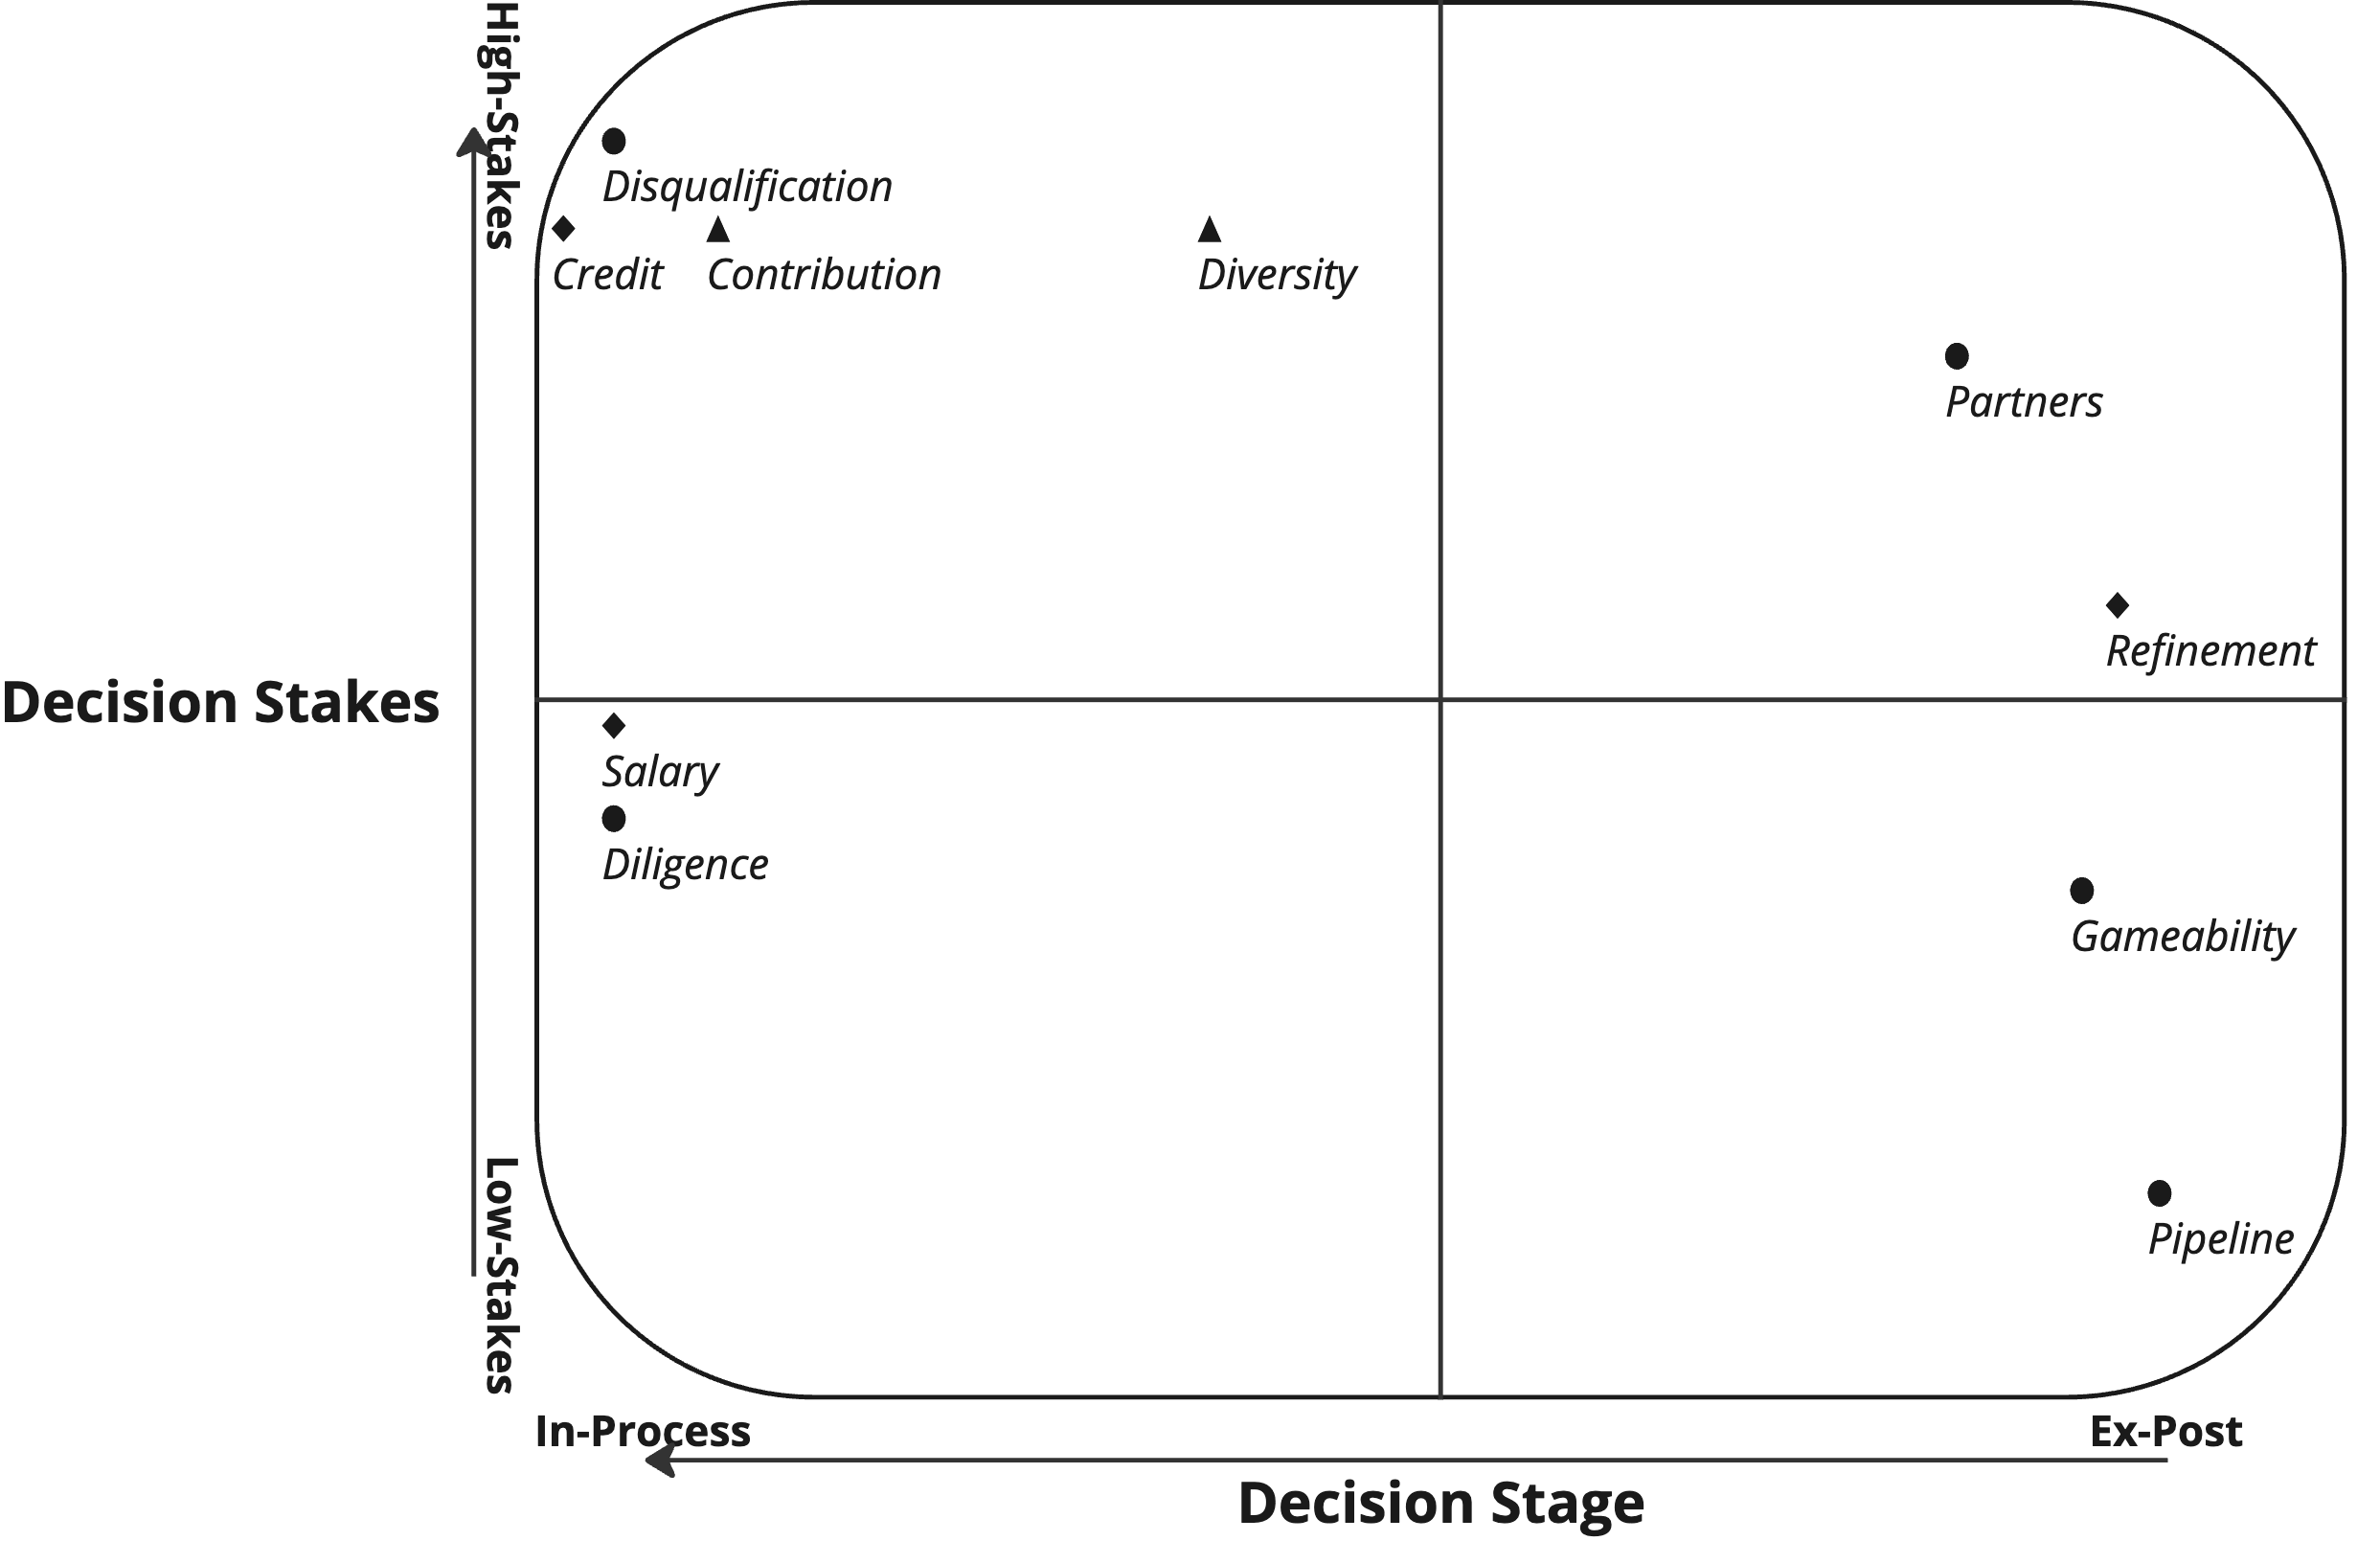
\includegraphics[width=0.8\textwidth]{context/full_decision_matrix.png}
  \caption{This figure places the decisions from Table \ref{tab:full_decision_list} on the Decision Matrix.}
  \label{fig:full_decision_matrix}
\end{figure}
\begin{savequote}[8cm]
    We caution against blindly embracing post-hoc notions of interpretability, especially when optimized to placate subjective demands. In such cases, one might - deliberately or not - optimize an algorithm to present misleading but plausible explanations.
  \qauthor{Zachary Lipton \cite{Lipton}}
\end{savequote}

\chapter{\label{ch:xai}XAI: Misleading In-Process, but Useful Post-Hoc}\blfootnote{This chapter is based a paper written in concert with Reuben Binns, Ulrik Lyngs, and Nigel Shadbolt. The paper is currently under review as: Neil Natarajan, Reuben Binns, Ulrik Lyngs, Nigel Shadbolt. 2024. “XAI: Misleading In Process, but Useful Post Hoc.” Under review at CHI 2025.}

% Notes
% Can we replicate misleading explanations? We have data from this year and last.
% Are there classes of cases which are plausibly connected to the types of areas that the old non-SHAP decision-making process would have yielded? Can we independently identify these in the new cohort?
% Maybe: does the new “SHAP” process reduce surprise/disagreement with the algorithm
% Can we do something qualitatively?
% How does SHAP have the right kind of effect on decision-making
% Could we measure the magnitude of disagreement between humans and algorithms?
% Then qualitatively, ask people why they disagreed with algorithm scores?
% It’s hard to tie this stuff specifically to the under/over-reliance stuff unless we can argue that more disagreement is good
% We don’t have ground truth, so the misleading stuff is difficult, but we can argue that disagreement/engagement are both good. We can qualitatively compare the richness/level of understanding/ perceived helpfulness.
% Do they have more reasons for disagreeing? More specific reasons?
% Fundamental thought: if SHAP helps the decision makers understand the reason why, but we don’t care about that factor, wouldn’t it be better to change the model so as to not consider that factor as much? Maybe explanation tools are a way of modifying the model here? Can the case study / utility be a change to the model? Maybe decision-makers need to be in the middle of their decision-making process to reconsider the principles, and maybe these decisions are best made using SHAP?
% Alternative case study idea: maybe various reviewers meet and extract generalisations from the SHAP charts they’ve been using?
% The idea of individual justice: no set of criteria exists that correctly applies to every case; under this principle, the value of SHAP is to say that “this particular case is an exception to the model, since you don’t want to mess with it in general, you just want to make an exception in this case”
% The underlying model is trying to predict accept/reject based on previous candidates, which is sort of a ground truth, but not the only truth that decision-makers are interested in; this is a major difference from the misleading explanations thing
% Another major difference: decision-makers have access to a lot of information the model doesn’t; part of the role of SHAP is to tell decision-makers when that info is important
% It sounds like the evaluation is qualitative / not-based-on-ground-truth. It’s instead based on decision-maker feedback about when they rely on the explainer system
% More satisfying to have some case study
% Can I collect with/without SHAP information on how they collect decisions?
% Could we apply SHAP to previously made decisions and use SHAP to elucidate the past year confusions? This was a part of the design process
% Does this necessarily need to be qualitative?
% Also: do we want to change the model next year based on the decisions made with this algorithm? I.e., should we rely more or less on specific features? This is sort of necessarily qualitative. Also, this could be taken from the design process, since this happened in the interviews
% This makes a good argument for why we can’t just do an RCT 

\minitoc

\section{Motivation}
In exploring the array of decision support tools applicable to global scholarship selection, explainable AI (xAI) offers a natural starting point. XAI tools are often offered as a fair and responsible way to support a decision-subject's right to explanation, empowering them while improving decision-making in potentially sensitive fields \cite{Goodman_Flaxman_2017}. A wealth of research within and without explores and evaluates xAI in these contexts \cite{molnar_interpretable_2019,barocas_hidden_2020,wachter_counterfactual_2017,Barocas_Hood_Ziewitz_2013,raghavan2020mitigating}. Despite this, much of this research cautions against blind applications of these tools to decision-making processes \cite{Lipton,miller_explainable_2023,kumar_problems_2020,Bastounis_Campodonico_vanderSchaar_Adcock_Hansen_2024}. In this chapter, we explore the potential for post-hoc notions of interpretability in supporting selection-related decision-making processes, and consider the potential for these tools to be applied in different supporting contexts.

\section{Introduction}
Despite the promise of xAI in enabling fair and explainable decision-making \cite{Goodman_Flaxman_2017}, Post-hoc xAI systems are oft as poor tools for decision support. \textcite{Lipton} cautions that well-intentioned explanation design may yield ``misleading but plausible'' explanations, and \textcite{miller_explainable_2023} notes that these post-hoc xAI methods provide justification for the underlying AI models and their outputs rather than allowing users to make their own informed decisions \cite{miller_explainable_2023}. This has, in recent years led to a shift away from post-hoc xAI entirely \cite{Lipton,miller_explainable_2023,kumar_problems_2020,Bastounis_Campodonico_vanderSchaar_Adcock_Hansen_2024}. The core of both critiques is that explanations may induce misplaced explainee trust in model outputs. Indeed, there is evidence that such xAI systems do induce trust in the underlying model \cite{lai_human_2019,jacobs_how_2021}. In response, research using xAI as a decision support tool (DST) often eschews post-hoc, model-agnostic explanations in favour of new paradigms such as \textcite{miller_explainable_2023}'s evaluative AI for decision-makers and \textcite{karimi_algorithmic_2021}'s causal models for decision subjects.

But have we been too hasty in rejecting these older methods? Underlying this shift away from xAI is the assumption that approaches will be deployed to increase trust in particular outputs in decision support contexts, even though such trust may be unwarranted when outputs are wrong. But is this always the case? Might these trust-inducing xAI be usefully deployed elsewhere, such as for post-decision evaluation of models and decision making processes?

We introduce a \emph{decision stage} distinction to help consider the benefits and risks of post-hoc interpretability tools as DSTs. We distinguish between: the \emph{in-process} stage, where AI outputs and post-hoc explanations are used to support human decision-makers in confirming or overriding the `primary' decision the model output advises on, and the \emph{ex-post} stage, where the primary decision has already been made, and the xAI is offered to inform second-order decisions about the decision-making process. (E.g., between application cycles, recruitment and selection practitioners examine their prior decision-making procedures and seeks to make decisions that improve them for the next cycle \cite{li2020hiring}.) We seek to answer two research questions (RQs):

\begin{enumerate}
    \item[(RQ1)] Do post-hoc explanations, when used as \emph{in-process} DSTs, induce unwarranted trust in the explainee?
    \item[(RQ2)] If post-hoc xAI methods induce unwarranted trust \emph{in-process}, could they still be useful \emph{ex-post}?
\end{enumerate}

At the \emph{in-process} stage, we run an online study to discern whether the problem of unwarranted trust is specific to xAI. We investigate \textcite{lundberg_unified_2017,ribeiro_anchors_2018}'s popular methods, SHapley-based Additive exPlanations (SHAP) \cite{lundberg_unified_2017} and Scoped Rules (Anchor) \cite{ribeiro_anchors_2018}, respectively, to see if they induce unwarranted trust. We also investigate a `Confidence' explanation consisting of the model's confidence statistic to determine if the problem of unwarranted trust is unique to explanations per se, or applies more generally to the presentation of any information that could increase positive perceptions of the AI's performance. We ask participants to \emph{estimate a person's salary} \cite{kohavi_scaling_1996} or \emph{predict whether someone will be severely delinquent in making a credit payment} \cite{GiveMeSomeCredit} with the help of an AI output and with or without an explanation. We find that SHAP explanations do increase unwarranted trust in AI outputs, but that Confidence does as well. We find no such effect for Anchor. This suggests the problem of unwarranted trust is not unique to xAI per se, and is rather a symptom of generic post-hoc justifications.

Having identified a core problem with some kinds of \emph{in-process} xAI, we consider whether they have any potentially redeeming features if deployed at the \emph{ex-post} level through a series of participatory design workshops. We refine our attention to SHAP because critiques by \textcite{Lipton} and \textcite{miller_explainable_2023} apply most squarely to it. We contend that, in an \emph{ex-post} context, this induction of unwarranted trust is less problematic, as primary decisions have already been made and thus trust in the AI outputs is not at issue. We ask participants to \emph{refine a scholarship selection algorithm} with the help of SHAP-based explanations. Through these workshops we find that, while SHAP explanations may induce unwarranted trust in specific model outputs, they can still be useful to drive process change in organisations.

Our primary contributions in this piece are:

\begin{enumerate}
    \item Quantitative findings indicating that the problem of explanation-induced unwarranted trust extends to generic post-hoc justifications, but that such criticism only applies \emph{in-process}.
    \item Qualitative findings that post-hoc explanations, properly presented, can make useful \emph{ex-post} DSTs.
\end{enumerate}

\section{Background}
\subsection{A Brief History of Explainable AI}\label{ssec:history}
\textcite{ribeiro_why_2016}'s Local Interpretable Model-agnostic Explanations (LIME), which identifies important features (creating a `feature-based' explanation) grew popular as an offering for explanations of Computer Vision (CV) models. \textcite{ribeiro_why_2016} demonstrated the explanation method on a task classifying huskies and wolves. By highlighting that the model used snow to recognise huskies, LIME would help a user spot what portions of an image were likely to be causing the model's classifications. By highlighting that the model used snow to recognise huskies, rather than e.g. their coat pattern, the user might come to understand the model's abilities and limitations, and calibrate their trust accordingly.

The explanation paradigm established by LIME was shortly thereafter applied to non-CV tasks. Tasks based on tabular data, in particular, were often explained using LIME \cite{zerilli_explaining_2020}. Subsequent xAI methods have revised the feature-centric paradigm established by LIME to better fit this new data type. \textcite{lundberg_unified_2017}'s SHAP offers another way of calculating the influence of each feature wherein the sum of the influences of each feature (plus a `bias' term) equals the model's output, and has since grown ubiquitous in the xAI field \cite{weerts_human-grounded_2019}.

But while the feature-based methodology underlying LIME and SHAP is useful for identifying error in the computer vision case, this relies on the human evaluator comparing explanation outputs to their (at least partial) knowledge of the ground truth (i.e., when the LIME explanation highlights a portion of the image, the human evaluator must rely on their knowledge of the ground truth to identify whether what is highlighted is relevant). While this may make good sense in cases such as the task classifying huskies and wolves, more contentious applications involve less obvious decisions where, even with access to feature space, a human reviewer might not be able to deduce the correct ground truth classification \cite{kumar_problems_2020,markus_role_2021}.\footnote{This is just one of many problems with feature importance explanations. \textcite{miller_explanation_2017} outlines a list of desiderata that model interpretability methods should satisfy; he points to a need for: contrastive, counterfactual, selective, and social explanations; the feature importance statistics yielded by LIME and SHAP are none of these.} But if these explanations are provided in cases where they do not help users identify cases where the AI output is incorrect, they can only serve to increase trust in the outputs, and cannot serve to decrease said trust where it is not warranted; explanations of AI outputs should only be reassuring if they might have not been.

`Example-based' explanations respond to many of these critiques. \textcite{wachter_counterfactual_2017}'s Counterfactual Explanations (CE) presents an example counterfactual to the input, showing the user a similar feature value with a different model output. \textcite{mothilal_explaining_2019}'s DIverse Contrastive Explanations (DICE) operate similarly, presenting multiple intentionally diverse counterfactuals to give the explainee a better sense of the many ways that the feature space could be perturbed. These counterfactuals serve to give explainees a glimpse into local model behaviour – if the model behaves strangely in any of these similar examples, it is likely untrustworthy in the original instance. However, these explanations are not without their own critiques. In particular, counterfactual explanations are subject to a Rashomon effect; i.e., for any explainable point, multiple counterfactuals may be equally valid. \textcite{miller_explanation_2017} argues that xAI methods should be selective in what they show explainees so as to not overwhelm them, but if there are many valid counterfactuals, we must then choose between showing an explainee all counterfactuals and violating selectivity, or selecting only a few counterfactuals and biasing the explanations.

\textcite{ribeiro_anchors_2018}'s Anchor retains the contrastive benefits of CE without suffering the same Rashomon paradox. The algorithm yields a set of conditional statements that help bound the model's output in a region surrounding the actual point. Similarly, \textcite{ustun_actionable_2019}'s Actionable Recourse (Recourse) offers decision subjects rules guiding what they must change in order to receive a different determination. These explanations meet \textcite{miller_explanation_2017}'s selectivity maxim without ad-hoc simplifications.

\subsection{A Taxonomy of Explanation Algorithms}
In much of the xAI literature, descriptors such as ``post-hoc'' or ``model-specific'' are used to describe types of explainability. We provide a taxonomy of them here and in Figure \ref{fig:taxonomy}.

\begin{figure}[htbp]
    \centering
    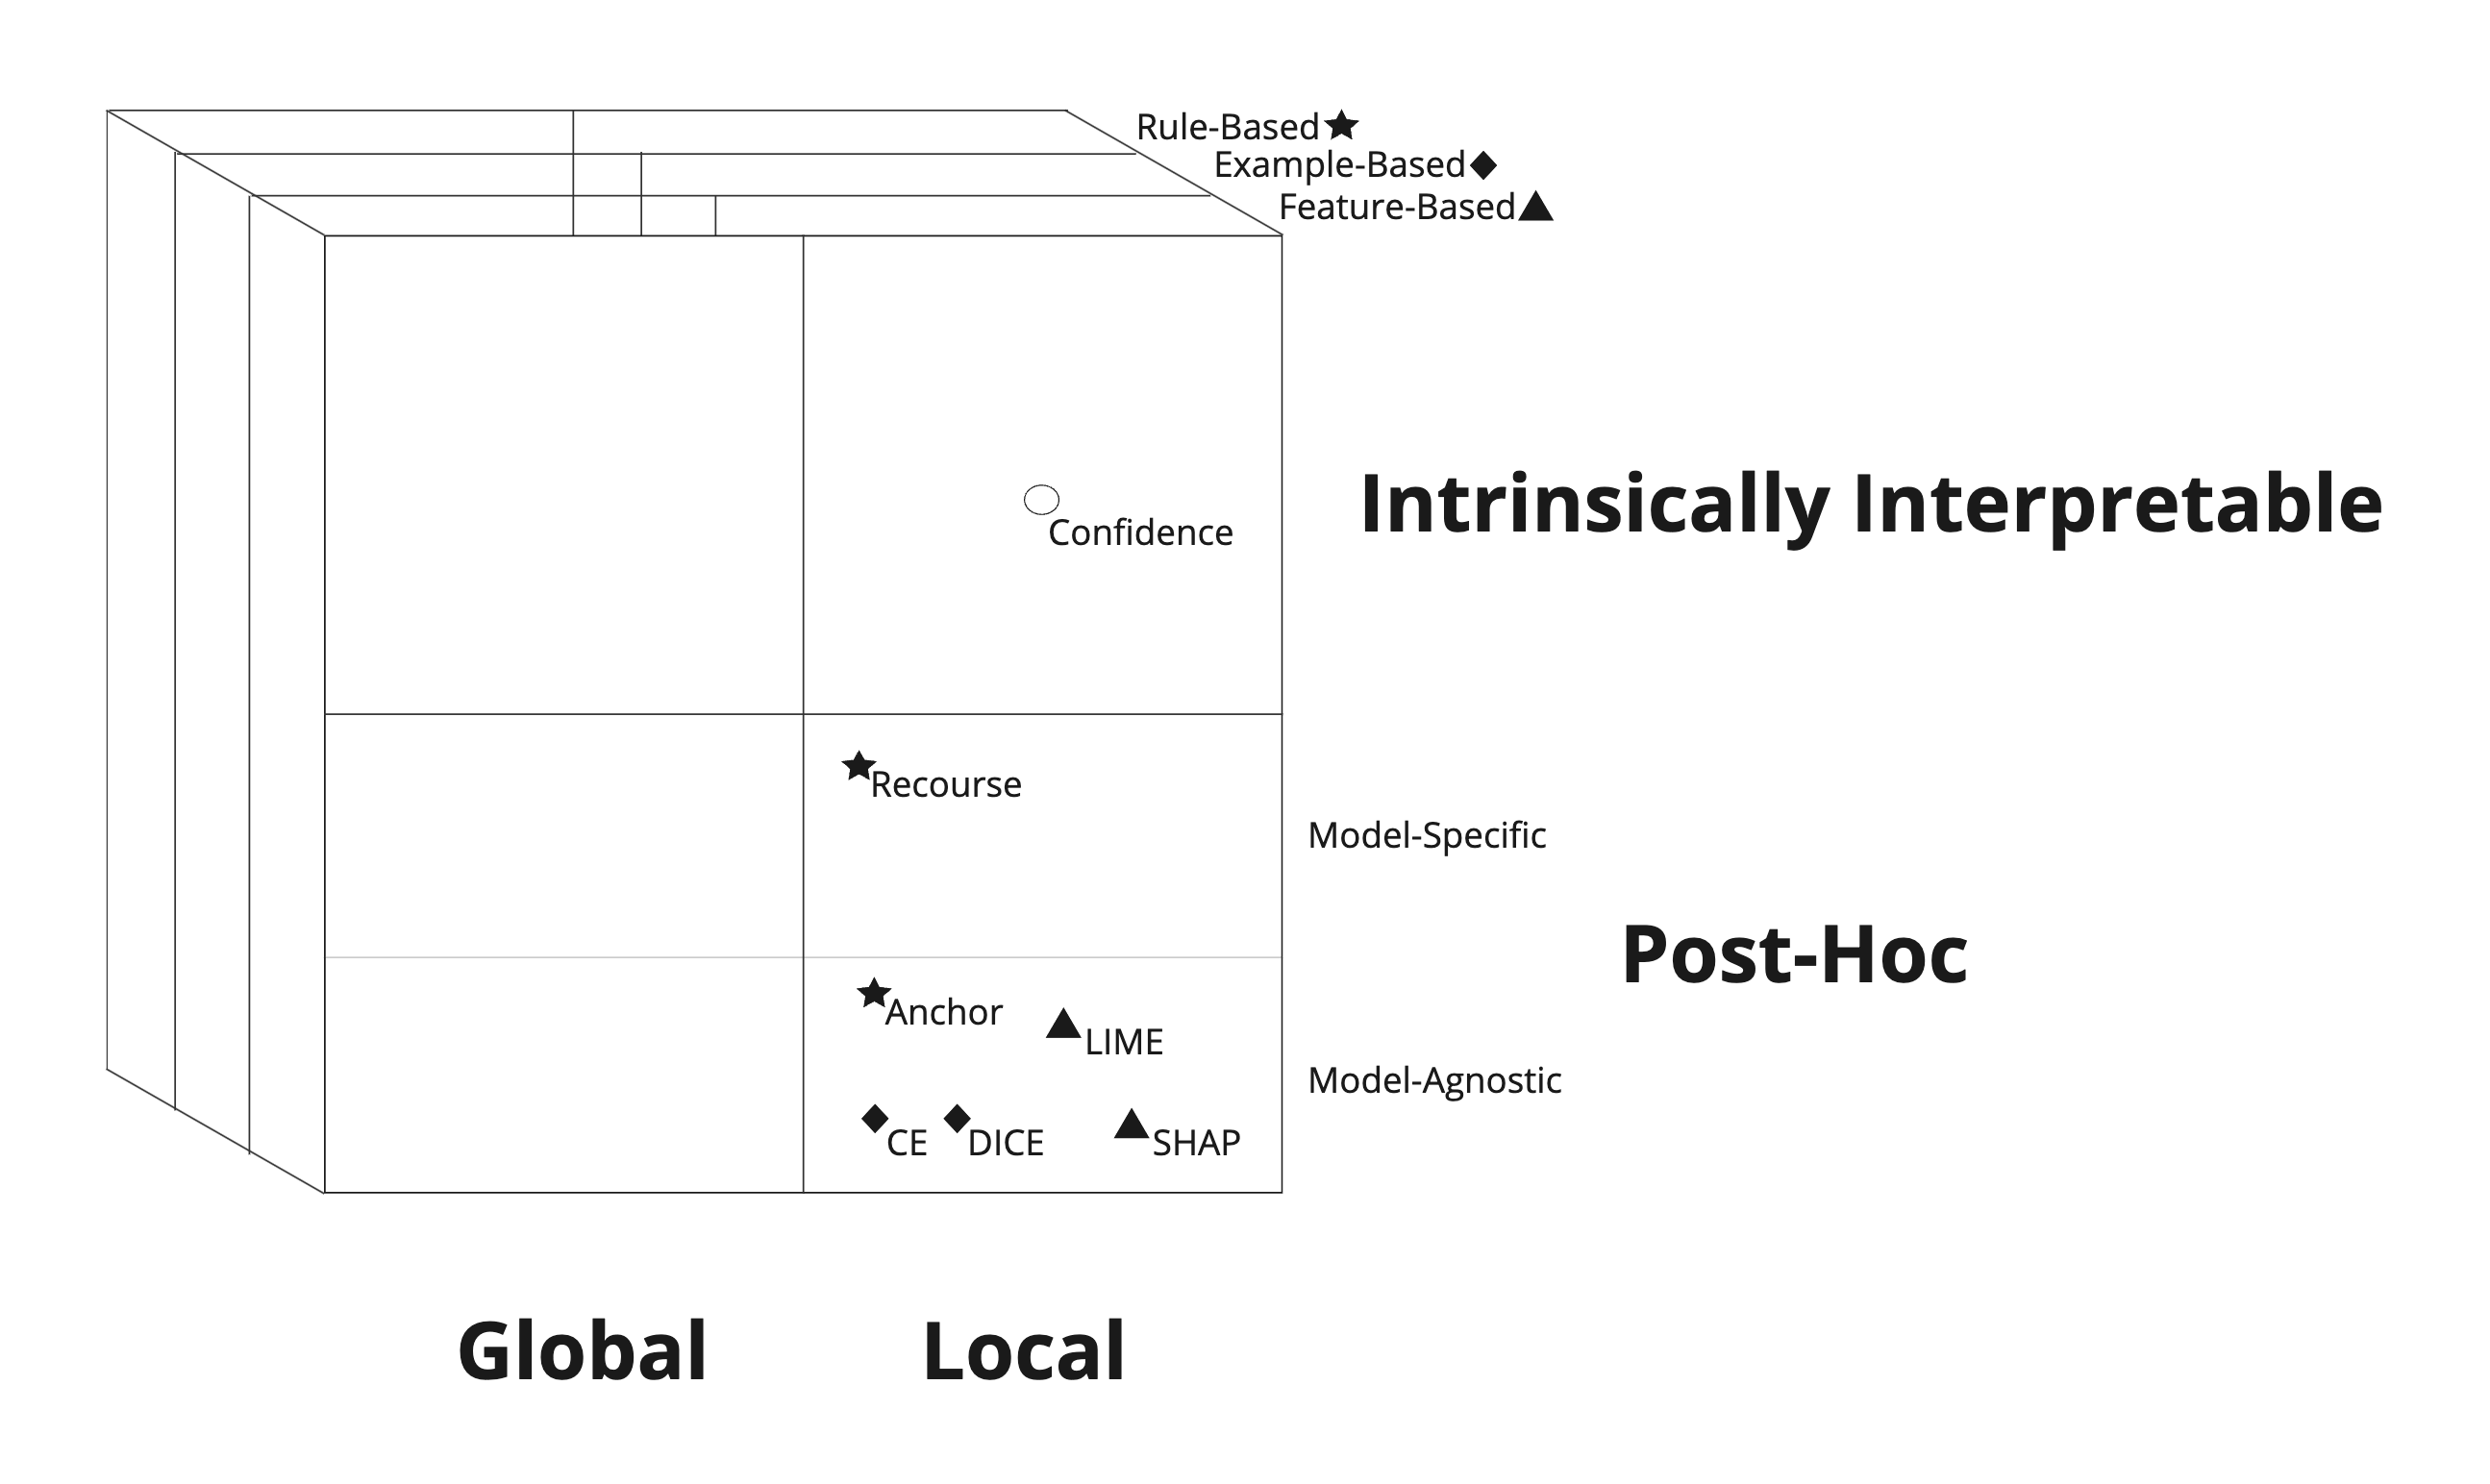
\includegraphics[width=.9\textwidth]{xai/taxonomy.png}
    \caption{Explainable AI methods are separated into types by this taxonomy. We focus primarily on kinds of post-hoc (model-agnostic) explanations, and highlight a number of explanations following different philosophies (SHAP and Anchor are of particular interest, as both recur in our analyses), but we also consider model confidence statistics, which follow none of these philosophies.}
    \label{fig:taxonomy}
\end{figure}

We begin by broadly categorising the space of explainable AI into two subgroups: intrinsically interpretable models and post-hoc explanations \cite{molnar_interpretable_2019}. Though intrinsically interpretable models offer solutions for interpretability and often present their own explanations, we (and the xAI critiques we engage with) focus primarily on post-hoc explanations. Key here is that, while intrinsically interpretable models are inherently model-specific, post-hoc methods may reap the benefits of model-agnosticity; thus, a single method may be used on any number of underlying models. This feeds into many of the main criticisms – \textcite{Lipton}'s argument about misleading explanations restricts itself to post-hoc models, we contend, because of this frequent ignorance about the model's internal processes.

Alternatively, explanations can be separated into global methods, which explain entire models, and local methods, which explain individual decisions \cite{molnar_interpretable_2019}. Though similar, the distinction between local and global differs from our \emph{decision stage} distinction as the decision stages distinction does not identify the scope of the explanation itself, but rather identifies the scope of the decision. Local explanations, of course, lend themselves best to \emph{in-process} decisions, but one could supply a global explanation here instead. And \emph{ex-post} decisions are varyingly informed best by local or global explanations. We focus on local explanations.

Finally, explainability methods could be instead subdivided by the design philosophy of their outputs \cite{friedrich_taxonomy_2011}. Some methods are `Feature-Based' in that they offer feature importance statistics. Other `Example-Based' explanations give examples. Yet other `Rule-Based' explanations offer rules that guide decision-making. Many explanations follow none of these paradigms. Model confidence statistics, for example, do not subscribe to any such design philosophies, but are often used as explanations in place of explainable AI systems \cite{zhang_effect_2020}. All explanations we mention, as well as where they fit on this taxonomy, are detailed in Figure \ref{fig:taxonomy}.

\subsection{Ethical Considerations of Employing xAI Systems as DSTs}
Researchers bring up many concerns about using AI systems in general as DSTs. The most relevant bodies of concern for us come from literature around scholarship selection and recruitment. One major concern is that AI algorithms amplify human biases \cite{MikePerkins_JasperRoe_2023}. Though this concern does and should limit applications of certain AI systems, it must be weighed against pre-existing human bias in pipelines. That is, a system might be less biased than what it replaces. Furthermore, a system might even be used to help holistic reviewers identify and mitigate their own biases \cite{alvero_ai_2020}.

More broadly, \textcite{alvero_ai_2020} note that, while AI researchers tend to think of fairness on a population level, recruiters (and, we contend, practitioners in related fields) think of fairness on an individual level. I.e., when making decisions based on qualitative information about a candidate in a process known as holistic review, reviewers are thinking of being fair to the candidate in front of them. But new AI tools blur the quantitative and the qualitative: what was once a simple score can now be a full explanation, and what was once a human-gradable essay could be automatically given a score. There is, we contend, space in these processes for tools that can help reviewers understand the qualitative and quantitative contexts surrounding the decisions they make.

\subsection{Evaluating Unwarranted Trust in a Model}
In order to evaluate whether an explanation induces unwarranted trust, we must evaluate both trust and warrantedness. We begin with trust. \textcite{jacovi_formalizing_2021} define trust in an AI system as characterised by two properties: ``the vulnerability of the user, and the ability to anticipate the impact of the AI model's decisions''; \textcite{vereschak_how_2021} similarly isolate three elements: ``trust is linked to a situation of vulnerability and positive expectations, and is an attitude''; \textcite{lee_trust_2004} give a similar definition of trust: ``An attitude that an agent will achieve an individual's goal in a situation characterized by uncertainty and vulnerability''. In all definitions, we see \emph{vulnerability} emerge as a key concept, and we variably also see that trust is characterised by \emph{uncertainty} and \emph{expectations}. Finally, we see that the definitions used with respect to evaluations of AI systems tend to be attitudinal in nature. However, though \textcite{vereschak_how_2021} suggest that trust is an unobservable variable, they term behaviours emergent from trust, rather than the attitude itself, `reliance'. 

The form of trust detailed by \textcite{vereschak_how_2021} is elsewhere called `attitudinal' trust \cite{crites_measuring_1994}. This form of trust is the one most often considered in human-centred AI, and much of the research discussing explainable AI focuses on this form of trust \cite{vereschak_how_2021, ford_play_2020, bansal_does_2021, yin_understanding_2019}. However, less frequently documented is a second, `behavioural' form of trust \cite{crites_measuring_1994}. When \textcite{jacovi_formalizing_2021,lee_trust_2004} argue that trust is measurable through such behaviours as reliance, we contend that they are speaking not of attitudinal trust, but rather of behavioural trust. Unlike attitudinal trust, behavioural trust does not rely on the participants' understanding of the term matching academic definitions, or on their estimates of their own trust accurately capturing what we seek to measure \cite{jacovi_formalizing_2021}. This more closely maps onto how explanations impact on the actual decisions made by humans-in-the-loop in practice.

Though attitudinal and behavioural trust are conceptually similar, research is mixed on the existence and strength of correlation between the two constructs \cite{ahmed_relationship_2009, kim_relation_2018}. As we wish to take a full account of trust in AI systems, we must consider both forms of trust.

We now turn to the warrantedness of said trust. \textcite{Vereschak_Alizadeh_Bailly_Caramiaux_2024} establish a clear distinction between trust and trustworthiness, and observe this distinction in decision-makers and decision subjects alike. That is to say, all parties involved agree that it is at least possible to place unwarranted trust in an algorithm \cite{Vereschak_Alizadeh_Bailly_Caramiaux_2024}. However, when it comes the the question of whether a given model output is trustworthy, opinions are more mixed. Some argue that certain uses of AI systems are inherently untrustworthy, but for many others, the trustworthiness of these systems is merely a matter of their accuracy \cite{Rebitschek_Gigerenzer_Wagner_2021}. \textcite{Rebitschek_Gigerenzer_Wagner_2021} find that, in the aforementioned case of credit estimation, potential decision subjects tend to simply place higher accuracy requirements on their willingness to trust an AI system. \textcite{jacovi_formalizing_2021} similarly conclude that a model's trustworthiness is related to properties such as accuracy, robustness, and bias. However, unlike accuracy, a model may be trustworthy in some contexts, and not in others. I.e., a model may be sufficiently accurate so as to be trustworthy when used to give rough estimates, but insufficiently accurate for use in high-stakes decisions. In the case of specific instances of model outputs, though, the question of trustworthiness is more straightforward: when a system outputs a correct (or an incorrect) result, that result is trustworthy (or untrustworthy).

\subsection{A Taxonomy of Critiques}
There is a large body of studies that empirically evaluate xAI methods. In some cases, an xAI method is evaluated not with human subject experiments but rather with analysis of mathematical properties \cite{doshi-velez_towards_2017}. These critiques range from \textcite{kumar_problems_2020}'s argument that SHAP explanations lack desired properties like contrastiveness to \textcite{lundberg_unified_2017}'s argument that LIME's mathematical properties make it unsuited to tabular data.

However, while these evaluations are instructive in that they provide interesting new perspectives on technologies, they do not help us evaluate whether utilising these explanations as DSTs is problematic in practice. To determine this, we turn to evaluations that involve humans using an AI system to perform some task \cite{ribeiro_why_2016,ribeiro_anchors_2018, rader_explanations_2018, jacobs_how_2021, bansal_does_2021}. These critiques, either explicitly or implicitly, tend to evaluate the impact of explanations on (attitudinal or behavioural) trust in AI systems. We enumerate some in Table \ref{tab:studies}.

\begin{table}[htbp]
    \centering
    \caption{This table documents human-centric evaluations of the effects of different explanations types on trust and warrentedness of trust. Many studies find evidence that all Feature-Based explanations increase trust in AI outputs, while results are mixed for other explanation types, but warrantedness of trust is rarely explored.}
    \adjustbox{max width=\textwidth}{
    \begin{tabular}{p{0.2\linewidth} p{0.15\linewidth} p{0.2\linewidth} p{0.2\linewidth} p{0.2\linewidth}}
        \toprule
        Study & Domain & Explanation Philosophy & Explanation Effect on Trust & Explanation Effect on Warrantedness of Trust \\
        \midrule
        \textcite{lai_human_2019} & Deception Detection & Feature-Based, Example-Based, Model Confidence & Feature- and Example-Based explanations increase explainee trust & No increase in detected user trust when the model's outputs are incorrect \\
        \textcite{binns_its_2018} & Multiple Domains & Feature-Based, Rule-Based (Recourse), Example-Based & Example-Based explanations decrease participant trust in the fairness of AI outputs & Warrentedness not investigated \\
        \textcite{ford_play_2020} & Image Recognition & Example-Based & Explanation presence or style has no main effect on end-user trust & Warrentedness not investigated \\
        \textcite{jacobs_how_2021} & Clinical Treatment & Feature-Based, Others & Participants demonstrate behavioural trust in models in all cases & Feature-based explanations of incorrect recommenations induce unwarranted behavioural trust. \\
        \textcite{bansal_does_2021} & Sentiment Classification & Feature-Based (LIME) & No observed effect of explanations relative to baseline (with AI) condition & Warrentedness not investigated \\
        \textcite{mohseni_trust_nodate} & Fake News Detection & Feature-Based and Others & End-user trust clustered into profiles that evolve, either increasing or decreasing over time & Warrentedness not investigated \\
        \bottomrule
        \textcite{Spitzer_Holstein_Morrison_Holstein_Satzger_Kühl} & Architecture Style Classification & Free Text (LLM) & LLM explanations increase end-user trust & LLM explanations increase unwarranted trust \\
    \end{tabular}
    }
    \label{tab:studies}
\end{table}

Despite \textcite{Lipton}'s ``misleading but plausible'' critique, the verdict of these human-centric evaluations is mixed. \textcite{lai_human_2019,jacobs_how_2021} both find that their Feature- and Example-Based explanations increase explainee trust in AI outputs, but \textcite{binns_its_2018} find that Example-Based explanations actually decrease explainee trust in AI outputs. The answer, we must conclude, depends on the explanation, the target group, or even the domain \cite{mohseni_trust_nodate}. 

Among those studies that do find an explanation-induced trust, few consider whether this trust is warranted. Among those that do, evidence is mixed; while some find unwarranted trust in some cases, others find such no effect \cite{lai_human_2019,jacobs_how_2021}. Thus, we must ask: are we too hasty in moving away from these explanations? 

\section{Experimental Study: \emph{In-Process} Decision Support}\label{sec:online}
\subsection{Research Questions}
Our online study seeks to answer RQ1:

\begin{enumerate}
    \item[(RQ1)] Does post-hoc xAI used as an \emph{in-process} DST induce unwarranted trust in the explainee?
\end{enumerate}

To do this, we compare three alternate conditions: \textcite{lundberg_unified_2017}'s aforementioned SHAP explanations, \textcite{ribeiro_anchors_2018}'s Scoped-Rule-(`Anchor')-based explanation, that obeys contrastive, selective, and counterfactual paradigms for explanations, and a `Confidence' condition consisting of the model's intrinsic confidence measurement. We measure trust in the AI system in two ways: attitudinal trust, measured by a survey question, and behavioural trust, measured by the participant's decision to follow the AI system's recommendation. We also measure the change in trust from before to after the explanation, and compare this change across the three conditions. These measurements are done across two tasks. Each participant sees six cases, with the explanatory and task conditions held constant. Finally, we calculate the correlation between attitudinal and behavioural trust, and between the change in attitudinal and behavioural trust.

\subsection{Methodology}
\subsubsection{Participants}
Participants were recruited via Prolific Academic's standard sampling method restricted to the United States.\footnote{\url{www.prolific.co}} They were paid at a rate of \$15 per hour. Participants were first shown an information sheet detailing the study's methodology and what was being asked of them. They were then asked to give informed consent. After consenting to participate in the study, participants were routed to Formr, our chosen survey design and hosting platform, to complete the online study.\footnote{\url{www.formr.org}} All data collected was anonymous and was stored on secure servers. Ethics review was performed by University of Oxford's Central University Research Ethics Committee.

\subsubsection{Tasks}
We restrict our research question to tasks familiar to lay people with a well-defined but difficult-to-ascertain ground truth. Our two tasks are chosen from a gamut of well-known algorithmic decision-making tasks as two particularly related to our third task, \emph{Refinement} (see Section \ref{sec:xaicase}) \cite{10.1111/j.1467-954X.2007.00740.x,Pasquale_2006,Latzer_Hollnbuchner_Just_Saurwein_2014}: \emph{estimating a hypothetical person's salary} based on census information of that individual, and \emph{predicting whether someone will be severely delinquent in making a credit payment}. We use two datasets: the Adult dataset collected from the 1994 US Census for the former task and the Give Me Some Credit dataset for the latter task \cite{kohavi_scaling_1996, GiveMeSomeCredit}. In both tasks, the participant aims to accurately estimate the dependent variable with the help of the AI system and one of several possible explanations of the AI system's estimate (which is possibly just the confidence rating of the model). In our analyses, we index these tasks as \emph{Salary} and \emph{Credit}. Note that each participant only receives one task to complete throughout all 6 cases. 

\begin{figure}[htbp]
    \centering
    \begin{subfigure}[b]{0.45\textwidth}
        \includegraphics[width=\textwidth]{xai/survey-shap.png}
        \caption{SHAP explanations for \emph{Salary}}
        \label{fig:shapsalary}
    \end{subfigure}
    \hfill
    \begin{subfigure}[b]{0.45\textwidth}
        \includegraphics[width=\textwidth]{xai/survey-shap-2.png}
        \caption{SHAP explanations for \emph{Credit}}
        \label{fig:shapcredit}
    \end{subfigure}
    \medskip
    \begin{subfigure}[b]{0.45\textwidth}
        \includegraphics[width=\textwidth]{xai/survey-anchor.png}
        \caption{Anchor explanations for \emph{Salary}}
        \label{fig:anchorsalary}
    \end{subfigure}
    \hfill
    \begin{subfigure}[b]{0.45\textwidth}
        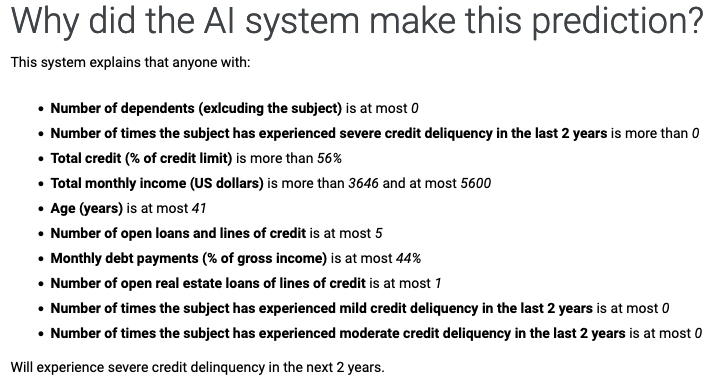
\includegraphics[width=\textwidth]{xai/survey-anchor-2.png}
        \caption{Anchor explanations for $credit$}
        \label{fig:anchorcredit}
    \end{subfigure}
    \medskip
    \begin{subfigure}[b]{0.45\textwidth}
        
\includegraphics[width=\textwidth]{xai/survey-confidence.png}
        \caption{Confidence explanations for \emph{Salary}}
        \label{fig:confidencesalary}
    \end{subfigure}
    \hfill
    \begin{subfigure}[b]{0.45\textwidth}
        
\includegraphics[width=\textwidth]{xai/survey-confidence-2.png}
        \caption{Confidence explanations for \emph{Credit}}
        \label{fig:confidencecredit}
    \end{subfigure}
    \caption{This figure shows sample explanations for all cases. Larger images and more detailed descriptions of explanations can be seen in Appendix \ref{app:figures}.}
    \label{fig:online_explanations}
\end{figure}

\subsubsection{Models}
In both tasks, we construct a predictor model using random forests and augment this predictor with three different explanatory conditions. Our random forest classifier achieves $86\%$ test accuracy on the Adult dataset and $93\%$ test accuracy on the Give Me Some Credit dataset. We use a SHAP explainer to produce one of our explanatory conditions, and an Anchor explainer to produce another; our final explanatory condition is an intrinsic explanation produced by the random forest model. Figure \ref{fig:online_explanations} shows sample explanations produced by these methods. These ultimately form three explanatory conditions: SHAP, Anchor, and Confidence. Note that each participant only receives one model of explanation throughout all 6 cases. 

\subsubsection{Design}
Both tasks rely on the same 3-between-by-2-within design using repeated measures to capture the same data before and after the presentation of each explanation. The between-subjects factor determines which model is used to generate the explanation a given participant will receive. The within-subjects factor is the repeated-measures `explanation presence' factor. This is either `before explanation' or `after explanation', indexed $before$ or $after$. A of the study design can be found in Figure \ref{fig:online_flowchart}.

\begin{figure*}[htbp]
    \centering
    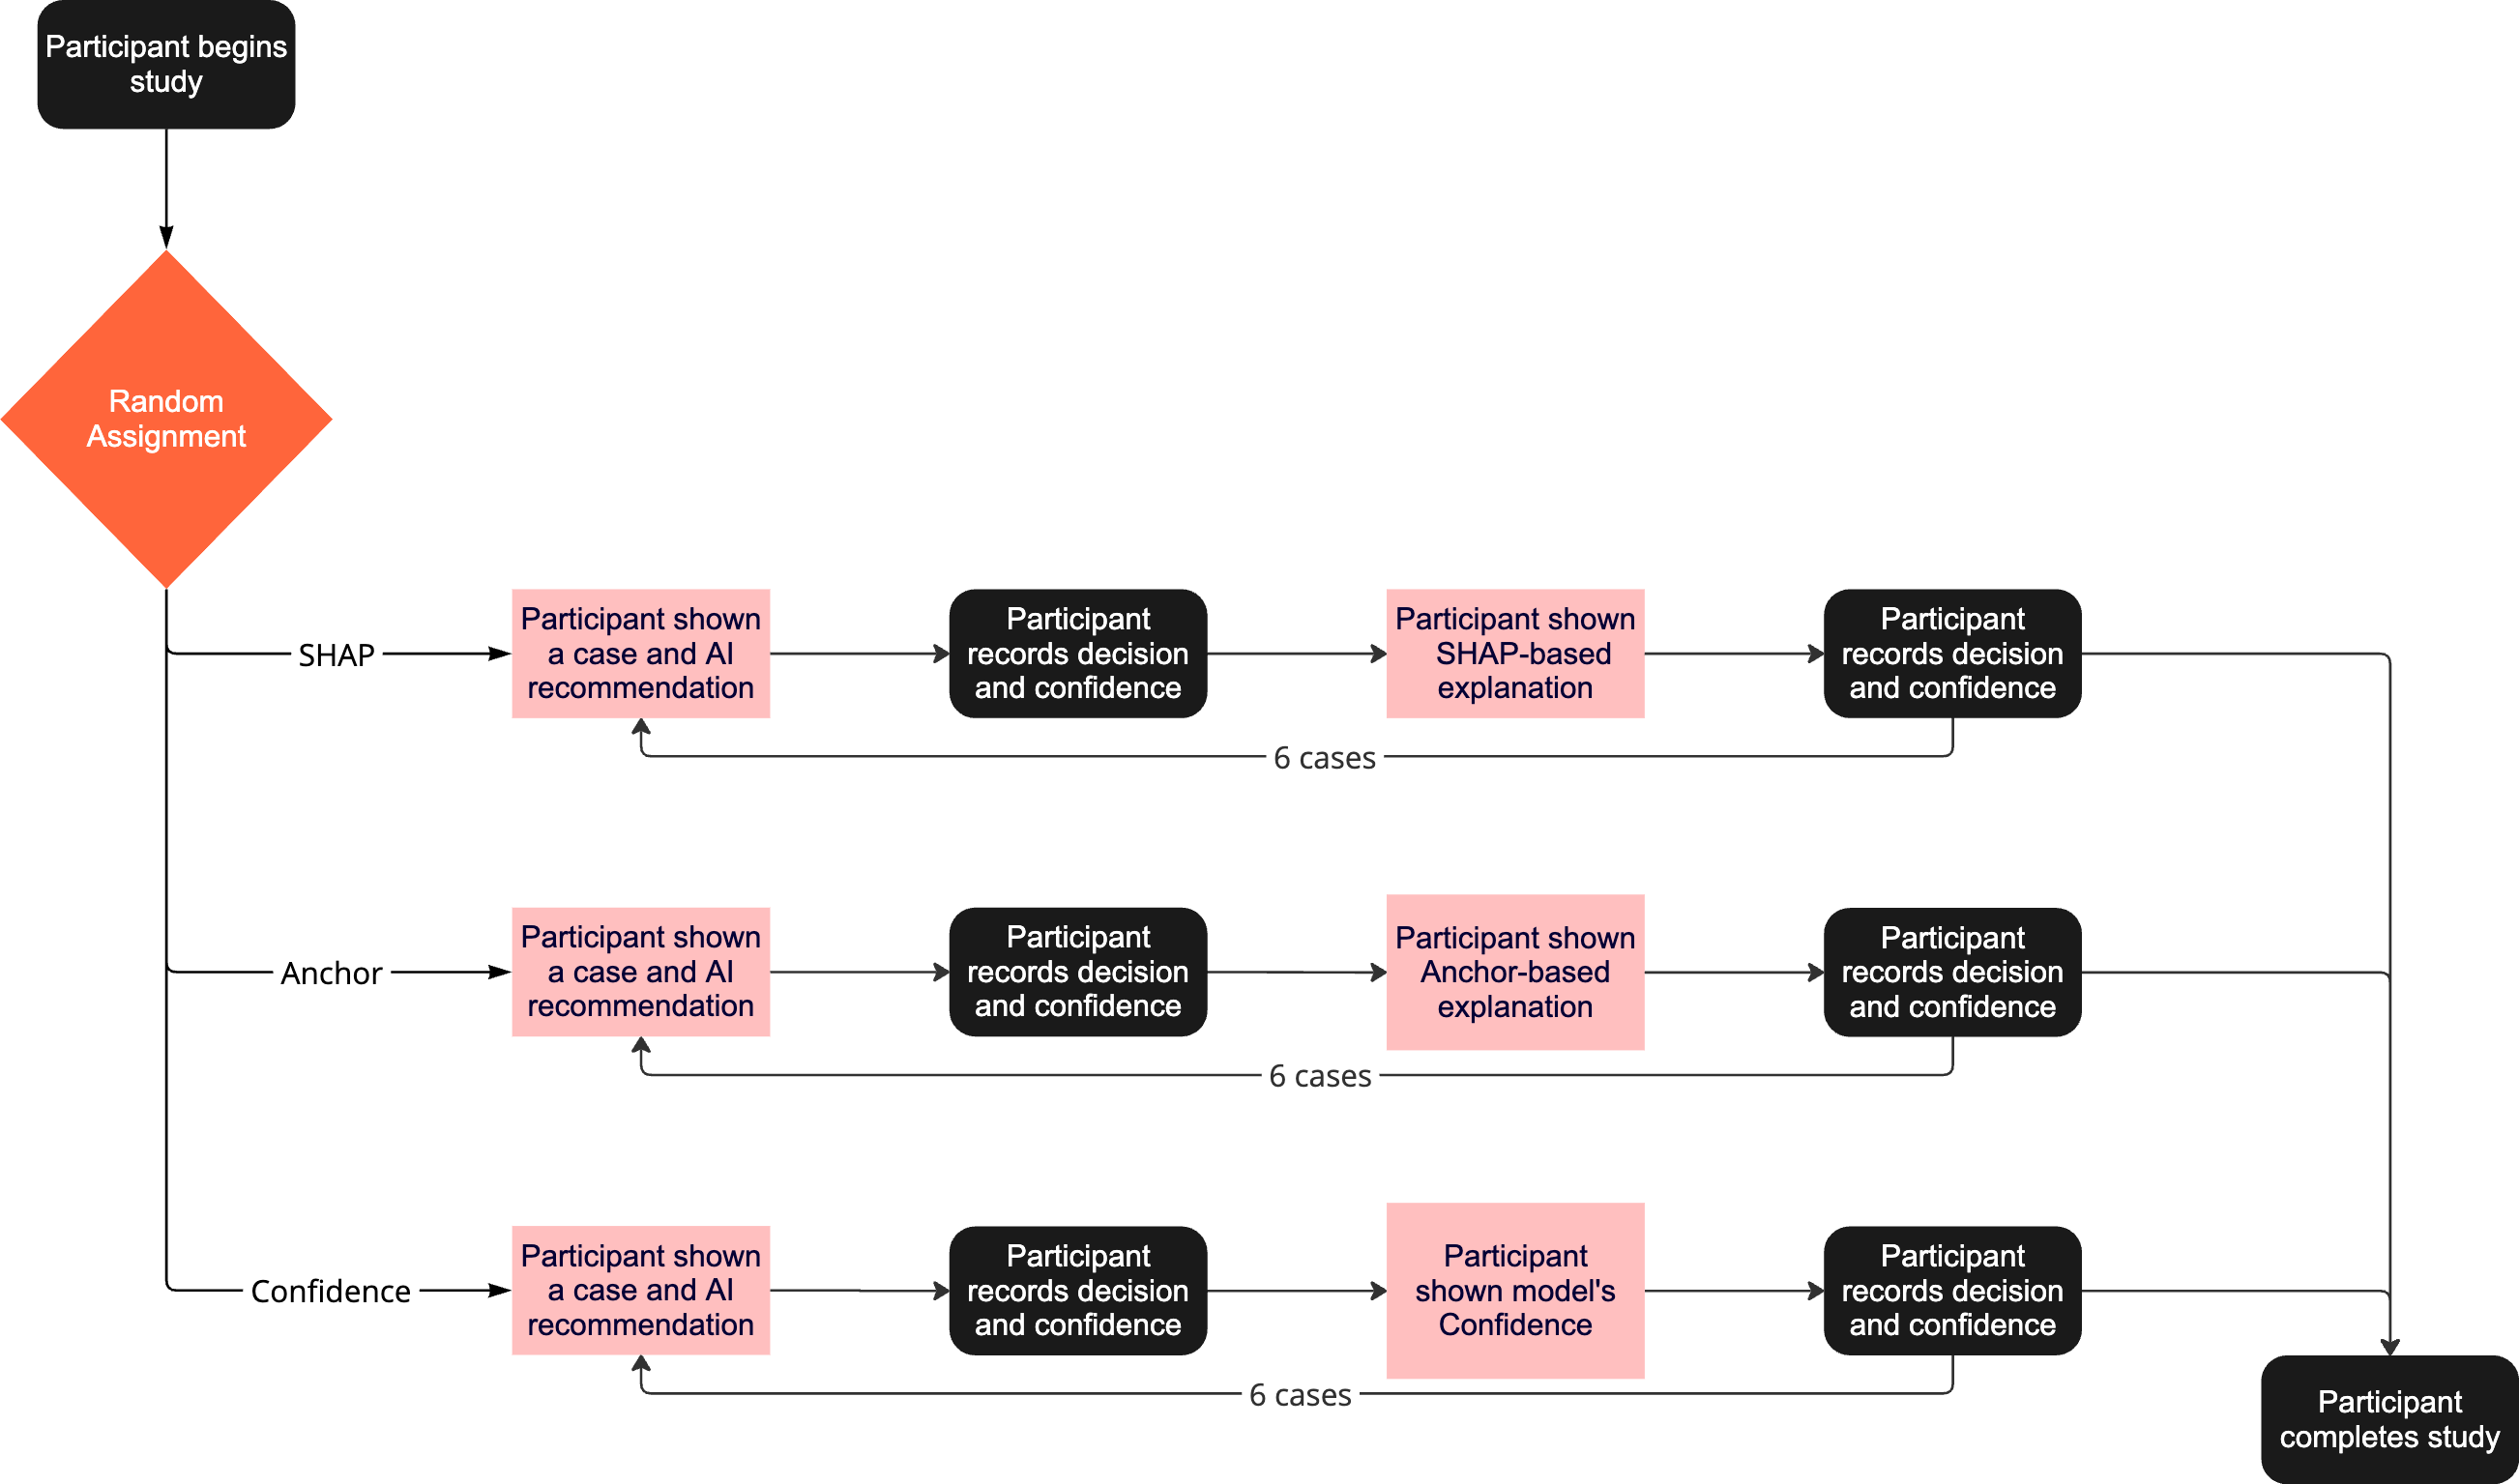
\includegraphics[width=\textwidth]{xai/online_flowchart.png}
    \caption{Participants in the online study are sorted into six buckets, where each bucket is segregated by explanatory condition and task and shown a brief description of the task (i.e., each participant sees only one of the explanations in Figure \ref{fig:online_explanations}). Then, each participant is shown 6 cases. In each case, participants are shown an applicant profile and a AI output. Participants are asked to agree or disagree with the AI output. Then, participants are given explanations based on their explanatory condition scores. They are then asked again to agree or disagree with the AI output.}
    \label{fig:online_flowchart}
\end{figure*}

\subsubsection{Questions and Variables}\label{sssec:q_and_v}
Each participant was shown a brief explanation of the task in question and was then asked to complete the 6 cases, with participants given a random mix of correct and incorrect cases. In each case, participants are first shown a table identifying subject of the case and an AI output of what determination they should make. They are then asked to estimate the dependent variable, and rate both their confidence in the estimate and their trust in the AI output on sliding scales (this is discretised to 20 points).

We code the participant's estimate as a binary $y_{human}$ variable:

\begin{equation}
    y_{human} := \begin{cases}
        \text{How much money does this person make?} & (Salary) \\
        \text{Will this person experience severe credit delinquency?} & (Credit)
    \end{cases}
\end{equation}

\noindent The two sliding scale responses are coded as $selfconfidence$ and $trust_{attitudinal}$ and have values between 1 and 20. These are defined:

\begin{equation}
    confidence := \begin{cases}
        \text{How confident are you in your estimation?} & (Salary) \\
        \text{How confident are you in your prediction?} & (Credit)
    \end{cases}
\end{equation}

\begin{equation}
    trust_{attitudinal} := \begin{cases}
        \text{How much do you trust the AI's estimation?} & (Salary) \\
        \text{How much do you trust the AI's prediction?} & (Credit)
    \end{cases}
\end{equation}

As we ask all questions in both the $before$ and $after$ conditions, we collect six responses from each participant in each case: $y_{human}^{before}$, $selfconfidence^{before}$, $trust_{attitudinal}^{before}$, $y_{human}^{after}$, $selfconfidence^{before}$, and $trust_{attitudinal}^{after}$.  We additionally have the binary variables $y_{True}$ and $y_{AI}$ that are the true value and the AI output of the dependent variable.

In addition to these, we define $agreement^{before}$ as:

\begin{equation}
    agreement^{before} := \begin{cases}
        1 & \text{if } y_{human}^{before} = y_{AI} \\
        0 & \text{otherwise}
    \end{cases}
\end{equation}

\noindent and $correct_{x}$ as:

\begin{equation}
    correct_{x} := y_{x} = y_{True}
\end{equation}

We define $trust_{behavioural}^{before}$ and $trust_{behavioural}^{after}$ to be the extent to which the participant's confidence agrees with the AI output:

\begin{equation}
    trust_{behavioural}^{x} := \begin{cases}
        confidence^{x}      & \text{if } agreement^{x} \\
        1-confidence^{x}    & \text{otherwise}
    \end{cases}
\end{equation}

Finally, in order to reason about the change in a variable due to the explanation, we define `$\Delta$' constructs for all variables with a $before$ and an $after$ as:

\begin{equation}
    \Delta variable := variable^{after} - variable^{before}
\end{equation}

\noindent so, e.g.:

\begin{equation}
    \Delta trust_{attitudinal} := trust_{attitudinal}^{after} - trust_{attitudinal}^{before}
\end{equation}

\subsubsection{Data Analysis}
We preregistered much of our analyses. Though we also include some post-hoc analysis below, we wish to delineate between the two types of analyses. The former are listed in full here.

We first wish to test for the presence of unwarranted trust. To do this, we measure the difference between ratings in each condition in the cases where the AI output is \textit{incorrect}, i.e. where $\neg correct_{AI}$. To do this, we run three one-sided t-tests \cite{caldwell_power_nodate} to determine:

\begin{equation}
    \Delta trust \geq 0 | \neg correct_{AI}
\end{equation}

\noindent for both $\Delta trust_{behavioural}$ and $\Delta trust_{attitudinal}$. Note that this is identical to repeated-measures t-tests on the the $trust_{behavioural}$ and $trust_{attitudinal}$ variables where $\neg correct_{AI}$. Following this, as this is also a between-subjects experiment, we wish to compare the varying effects of different explanation methods in this case. Thus, we run two between-subjects ANOVAs \cite{caldwell_power_nodate} on $\Delta trust_{behavioural}$ and $\Delta trust_{attitudinal}$ across the explanatory conditions again filtered on $\neg correct_{AI}$. When these ANOVAs have significant results ($p < 0.05$), we run Tukey's Honestly Significant Difference (HSD) test \cite{caldwell_power_nodate}.

Finally, in our Salary Estimation survey, we observed a strong positive correlation between our two trust variables, though we did not preregister it for that study. Indeed, correlation analysis is a well-documented method for confirming two measurements indeed measure the same concept \cite{westen_quantifying_2003, morata-ramirez_construct_2013}. Thus, we additionally included the calculation of Pearson's correlation between $trust_{behavioural}$ and $trust_{attitudinal}$ and between $\Delta trust_{attitudinal}$ and $\Delta trust_{behavioural}$ in our preregistration for the Credit Delinquency Prediction survey. 

\paragraph{Power Analysis}
We run power analyses using \textcite{caldwell_power_nodate}'s Superpower. Specifically, we desire sufficiently powerful results on our primary analysis. We select a moderate effect size of interest (Cohen’s $f$) of $0.15$ (yielding group means $-0.15$ and $0.15$ with unit variance), and target a power of at least $0.90$. We note that, using a one-way T-test at $p = 0.05$ and assuming a sample size of $200$, we get power far above $0.90$. We also test for the ANOVA assuming unit variance and group means of $-0.15$, $0.15$, and $0.15$. Under these conditions, we achieve a power of $0.90$ with $200$ samples per condition. We ask each participant a total of 6 questions, and the AI output is incorrect in slightly less than half of them. In order to achieve $200$ samples per condition, therefore, we aim to recruit a total of roughly $66$ participants per condition, or roughly $200$ participants in total.

\paragraph{Preregistration}
We have preregistered analyses for both of our tasks in the OSF registries \cite{natarajan_binns_2022}. 

\subsection{Results}\label{ssec:os_results}
In both tasks, though we originally set $200$ as our target participants, some participants did not complete our task following Prolific Academic's guidelines. Data from these participants was marked incomplete and removed from consideration. 

After this removal, we had a total of $192$ participants complete the Salary Estimation study. These were split randomly into our three explanatory groups. By gender, $115$ were Male, $76$ were Female, and $1$ did not provide gender information. By ethnicity, $137$ were white, $10$ did not provide ethnicity, and the remaining $45$ were split among non-white ethnicities. Our participants were an average of $36.7$ years old, with the youngest being $18$ and the oldest $74$. Each applicant completed an introductory page and six cases. The average completion time for these tasks was $7$ minutes $43$ seconds, the minimum was $2$ minutes $25$, and the maximum was $36$ minutes $46$.

We had a total of $197$ participants complete the Credit Delinquency Prediction study. These were similarly split into groups. By gender, $106$ were Male, $90$ were Female, and $1$ did not provide gender information. By ethnicity, $143$ were white, $11$ did not provide ethnicity, and the remaining $43$ were split among non-white ethnicities. Our participants were an average of $38.4$ years old, with the youngest being $20$ and the oldest $77$. Each applicant completed an introductory page and six cases. The average completion time for these tasks was $7$ minutes $53$ seconds, the minimum was $2$ minutes $17$, and the maximum was $30$ minutes $13$.

\subsubsection{SHAP and Confidence Increase Unwarranted Trust}
We first run the one-sided t-tests on the two trust variables ($attitudinal$ and $behavioural$). I.e., we test:

\begin{equation}
    \Delta trust_{x} > 0 | \neg correct_{AI} \text{ for } x \in \{behavioural, attitudinal\}
\end{equation}

\noindent for both \emph{Salary} and \emph{Credit} across SHAP, Anchor, and Confidence. A positive $F$ statistic here indicates $trust^{after} > trust^{before}$ and a negative $F$ statistic indicates $trust^{after} < trust^{before}$, but, as these are one-sided tests, $p$-values will only be meaningful when $F > 0$. This test was preregistered in both of our tasks \cite{natarajan_binns_2022}. Table \ref{tab:delta-trust-t} contains the results of these analyses.  

\begin{table}[htb]
    \centering
    \caption{These one-sided t-tests test for $\Delta trust > 0 | \neg correct_{AI}$ for all explanatory conditions and both tasks. We find that SHAP and Confidence increase unwarranted trust in the AI system.}
    \label{tab:delta-trust-t}
    \begin{tabular}{l l l r r}
        \toprule
        Task & Explanation & Variable & F Statistic & p Value \\ 
        \midrule
        \emph{Salary} & Anchor & $\Delta trust_{behavioural}$ & $0.509$ & $0.306$ \\
        & & $\Delta trust_{attitudinal}$ & $0.165$ & $0.434$ \\
        & SHAP & $\Delta trust_{behavioural}$ & $\mathbf{3.811}$ & $\mathbf{<0.001}$ \\
        & & $\Delta trust_{attitudinal}$ & $-0.886$ & $0.812$ \\
        & Confidence & $\Delta trust_{behavioural}$ & $\mathbf{2.196}$ & $\mathbf{0.015}$ \\
        & & $\Delta trust_{attitudinal}$ & $0.945$ & $0.173$ \\
        \midrule
        \emph{Credit} & Anchor & $\Delta trust_{behavioural}$ & $1.396$ & $0.082$ \\
        & & $\Delta trust_{attitudinal}$ & $-2.364$ & $0.990$ \\
        & SHAP & $\Delta trust_{behavioural}$ & $1.516$ & $0.066$ \\
        & & $\Delta trust_{attitudinal}$ & $\mathbf{2.475}$ & $\mathbf{0.007}$ \\
        & Confidence & $\Delta trust_{behavioural}$ & $\mathbf{1.835}$ & $\mathbf{0.034}$ \\
        & & $\Delta trust_{attitudinal}$ & $0.940$ & $0.174$ \\
        \bottomrule
    \end{tabular}
\end{table}

This indicates that SHAP and Confidence appear to lead users to trust the AI system more when that system is wrong. We find this result more strongly for behavioural trust than attitudinal trust in all but one test.

Notably, Anchor does not follow this pattern, and instead shows no significant increase in either attitudinal or behavioural trust on these one-sided t-tests. (However, as we explore in Section \ref{sec:anchor-attitudinal}, they may show a significant decrease.)

\subsubsection{Different Explanation Styles Have Different Effects on Unwarranted Trust}
We have shown already that SHAP and Confidence induce unwarranted trust relative to no explanation; we now show that there is significant difference in the effect of some explanatory conditions relative to others. To do this, we examine the $\Delta trust_{behavioural}$ and $\Delta trust_{attitudinal}$ variables across explanatory conditions with an ANOVA test. For this test, we filter on $\neg correct_{AI}$. I.e.:

\begin{equation}
    \begin{split}
        \Delta \text{ any}(trust_{x1,x2} \neq trust_{x1,x3}) | \neg correct_{AI} & \text{ for } x1 \in \{behavioural, attitudinal\} \\
        & \text{ and } x2,x3 \in \{SHAP, Anchor, Confidence\}
    \end{split}
\end{equation}

\noindent This test was preregistered in both of our tasks \cite{natarajan_binns_2022}. Table \ref{tab:delta-trust-anova} contains the results of these analyses.

\begin{table}[htb]
    \centering
    \caption{These ANOVAs compare $\Delta trust$ between SHAP, Confidence, and Anchor to indicate where significant differences exist. We find two statistically significant differences, indicating that we should focus post-hoc analyses on these two.}
    \label{tab:delta-trust-anova}
    \begin{tabular}{lrrr}
        \toprule
        Task & Variable & F Statistic & p Value \\
        \midrule
        \emph{Salary} & $\Delta trust_{behavioural}$ & $\mathbf{3.671}$ & $\mathbf{0.026}$ \\
        & $\Delta trust_{attitudinal}$ & $0.925$ & $0.397$ \\
        \midrule
        \emph{Credit} & $\Delta trust_{behavioural}$ & $0.066$ & $0.936$ \\
        & $\Delta trust_{attitudinal}$ & $\mathbf{6.213}$ & $\mathbf{0.002}$ \\
        \bottomrule
    \end{tabular}
\end{table}

Note from Table \ref{tab:delta-trust-anova} that in the Salary Estimation task, we find no significant results for our ANOVA $trust_{attitudinal}$, but do find significant results for $trust_{behavioural}$. However, in the Credit Delinquency Prediction task, we find significant results for our ANOVA $trust_{attitudinal}$, but none for $trust_{behavioural}$. We examine these two findings separately.

\subsubsection{SHAP Increases Behavioural Trust More than Anchor in the Salary Estimation Task}
We now show that:

\begin{equation}
    \Delta trust_{behavioural,SHAP,salary} > \Delta trust_{behavioural,Anchor,salary} | \neg correct_{AI}
\end{equation}

\noindent Note that, while the result of the ANOVA test in table \ref{tab:delta-trust-anova} supports that there is indeed a statistically significant difference in the three group means of the $\Delta trust_{behavioural}$ variable, it does not specify which means are greater and which are less. For an indication of which means are greater, following our preregistered protocol for significant ANOVA results, we turn to Tukey's Honestly Significant Difference (HSD) test as a post-hoc test in table \ref{tab:delta-trust-hsd}. As we found significant results in the ANOVA test of $\Delta trust_{behavioural}$ filtered on $\neg correct_{AI}$, we restrict our post-hoc analysis to this variable.

\begin{table}[htb]
    \centering
    \caption{Tukey's HSD test compares $\Delta trust_{behavioural,x}$ in \emph{Salary} with $\neg correct_{AI}$. We find that SHAP increases behavioural trust in incorrect AI outputs more than Anchor.}
    \label{tab:delta-trust-hsd}
    \begin{tabular}{lllrr}
        \toprule
        Explanation A & Explanation B & Variable & Test Statistic & p Value \\
        \midrule
        SHAP & Anchor & $\Delta trust_{behavioural}$ & $\mathbf{2.310}$ & $\mathbf{0.022}$ \\
        Confidence & Anchor & $\Delta trust_{behavioural}$ & $0.855$ & $0.599$ \\
        SHAP & Confidence & $\Delta trust_{behavioural}$ & $1.455$ & $0.198$ \\
        \bottomrule
    \end{tabular}
\end{table}

As can be seen in Table \ref{tab:delta-trust-hsd}, we observe a significant difference in the mean of $\Delta trust_{behavioural}$ between the SHAP and Anchor conditions with $\neg correct_{AI}$, but we do not observe a significant difference between the other conditions. This indicates that, beyond increasing behavioural trust in incorrect AI outputs, SHAP increases behavioural trust in incorrect AI outputs \emph{more} than Anchor.

\subsubsection{Anchor Decreases Unwarranted Attitudinal Trust Relative to SHAP and Confidence in the Credit Delinquency Prediction Task}
Note that we found a large negative F for $\Delta trust_{attitudinal}$ in the Anchor case in the Credit Delinquency Prediction portion of table \ref{tab:delta-trust-t} – an effect that is not significant due to the one-sidedness of our tests. However, as we found only positive F values for $\Delta trust_{attitudinal}$ in the SHAP and Confidence cases, we might expect that Anchor has a negative effect on $\Delta trust_{attitudinal}$ relative to SHAP and Confidence. Indeed, the result of the ANOVA test in table \ref{tab:delta-trust-anova} supports that there is indeed statistically significant difference in the three group means of the $\Delta trust_{attitudinal}$ variable in this task, though it again does not specify which groups are different, or how.

For an indication of which means are greater, following our preregistered protocol for significant ANOVA results, we turn again to a Tukey's HSD test as a post-hoc test in table \ref{tab:delta-trust-hsd-2}. As we found significant results in the ANOVA test of $\Delta trust_{attitudinal}$ filtered on $\neg correct_{AI}$, we restrict our post-hoc analysis to this variable. We test:

\begin{equation}
    \begin{split}
        & \Delta trust_{behavioural,x1,credit} > \Delta trust_{behavioural,x2,credit} | \neg correct_{AI} \\
        & \qquad \text{ for } x1,x2 \in \{SHAP, Anchor, Confidence\}
    \end{split}
\end{equation}

\begin{equation}
    \begin{split}
        \Delta \text{ any}(trust_{x1,x2} \neq trust_{x1,x3}) | \neg correct_{AI} & \text{ for } x1 \in \{behavioural, attitudinal\} \\
        & \text{ and } x2,x3 \in \{SHAP, Anchor, Confidence\}
    \end{split}
\end{equation}

\begin{table}[htb]
    \centering
    \caption{Tukey's HSD test compares $\Delta trust_{attitudinal}$ across explanations in \emph{Credit} with $\neg correct_{AI}$. We find that Anchor decreases unwarranted trust relative to SHAP and Confidence.}
    \label{tab:delta-trust-hsd-2}
    \begin{tabular}{lllrr}
        \toprule
        Explanation A & Explanation B & Variable & Test Statistic & p Value \\
        \midrule
        SHAP & Anchor & $\Delta trust_{attitudinal}$ & $\mathbf{1.213}$ & $\mathbf{<0.001}$ \\
        Confidence & Anchor & $\Delta trust_{attitudinal}$ & $\mathbf{1.030}$ & $\mathbf{<0.001}$ \\
        SHAP & Confidence & $\Delta trust_{attitudinal}$ & $0.183$ & $0.708$ \\
        \bottomrule
    \end{tabular}
\end{table}

As can be seen in table \ref{tab:delta-trust-hsd-2}, we observe a significant difference in the mean of $\Delta trust_{behavioural}$ between the Anchor condition and both other conditions, but we do not observe a significant difference between SHAP and Confidence. This indicates that, relative to both other conditions, Anchor actually \emph{reduces} attitudinal trust in the AI output.

Note that this does not prove that Anchor reduces attitudinal trust relative to no explanation. For this analysis, we will need another t-test. As we did not preregister this test, analysis of this phenomenon is included in exploratory analysis below.

\subsubsection{Behavioural and Attitudinal Trust are Highly Correlated}
It should be noted that some patterns observed for $trust_{behavioural}$ do not hold for $trust_{attitudinal}$ and vice-versa. However, while they are mathematically distinct constructs, they are both intended to measure the same underlying phenomenon. We apply Pearson's correlation analysis across all explanatory conditions in both the before- and after- cases. We also perform this analysis on $\Delta trust_{attitudinal}$ and $\Delta trust_{behavioural}$. 

For this analysis, we do not filter out positive cases. Rather, we consider all cases together. Results can be seen in table \ref{tab:trust-correlation}.\footnote{This analysis was only partially preregistered; we did not register this analysis in the Salary Estimation task, but we did in the Credit Delinquency Prediction task \cite{natarajan_binns_2022}.}

\begin{table}[htb]
    \centering
    \caption{Pearson's test shows a high correlation between $trust_{attitudinal}$ and $trust_{behavioural}$ in both tasks. This correlation extends to the relationship between $\Delta trust_{attitudinal}$ and $\Delta trust_{behavioural}$.}
    \label{tab:trust-correlation}
    \begin{tabular}{lllrr}
        \toprule
        Task & Variable A & Variable B & Rho & p \\
        \midrule
        \emph{Salary} & $trust_{attitudinal}$ & $trust_{behavioural}$ & $\mathbf{0.630}$ & $\mathbf{<0.001}$ \\
        & $\Delta trust_{attitudinal}$ & $\Delta trust_{behavioural}$ & $\mathbf{0.265}$ & $\mathbf{<0.001}$ \\
        \midrule
        \emph{Credit} & $trust_{attitudinal}$ & $trust_{behavioural}$ & $\mathbf{0.612}$ & $\mathbf{<0.001}$ \\
        & $\Delta trust_{attitudinal}$ & $\Delta trust_{behavioural}$ & $\mathbf{0.179}$ & $\mathbf{<0.001}$ \\
        \bottomrule
    \end{tabular}
\end{table}

Note that, though the attitudinal and behavioural variables display different behaviour in other analyses, table \ref{tab:trust-correlation} indicates that they are indeed highly correlated across both of our tasks. Furthermore, though the correlation between the $\Delta trust$ is more modest, it is still statistically significant. These together leave little doubt that $trust_{attitudinal}$ and $trust_{behavioural}$ measure related, and perhaps even identical, concepts. In other words, when a participant says they trust the AI output, they generally act accordingly.

\subsubsection{Anchor Decreases Attitudinal Trust in AI Outputs}\label{sec:anchor-attitudinal}
Having found no significant result indicating the presence of the hypothesised effect of Anchor explanations on unwarranted trust, we explore what effect Anchor explanations have on end users' trust in incorrect AI outputs. For the purposes of this analysis, we filter on $\neg correct_{AI}$.\footnote{This analysis was not preregistered.}

We noted already that SHAP and Confidence appear to increase trust in cases where the AI output is incorrect. However, we noticed no such result for Anchor. However, we did observe an apparent negative effect on $\Delta trust_{attitudinal}$ in the t-tests for the Credit Delinquency Prediction task, though, as the tests were one-sided, we could not confirm significance. Thus, we repeat this test as a two-sided test, as shown in table \ref{tab:delta-trust-t-2}. We also repeat other t-tests on Anchor as two-sided, though, as they all have positive F-values, note that none can yield significant results.

\begin{table}[htb]
    \centering
    \caption{Two-sided t-tests compare $\Delta trust_{x,Anchor} \neq 0 for x \in \{attitudinal, behavioural\}$ in both tasks. We find that Anchor explanations decrease attitudinal trust in incorrect AI outputs in \emph{Credit}, but all other results are inconclusive.}
    \label{tab:delta-trust-t-2}
    \begin{tabular}{lllrr}
        \toprule
        Task & Explanation & Variable & t Statistic & p Value \\ 
        \midrule
        \emph{Salary} & Anchor & $trust_{behavioural}$ & $0.509$ & $0.611$ \\
        & & $trust_{attitudinal}$ & $0.165$ & $0.869$ \\
        \midrule
        \emph{Credit} & Anchor & $trust_{behavioural}$ & $1.396$ & $0.164$ \\
        & & $trust_{attitudinal}$ & $\mathbf{-2.364}$ & $\mathbf{0.019}$ \\
        \bottomrule
    \end{tabular}
\end{table}

Note here that, on the two-sided t-test, we \textit{do} find a that the provision of Anchor explanations decreases participant attitudinal trust in incorrect AI output, at least in the Credit Delinquency Prediction task. However, we do not see a similar effect on behavioural trust. 

\subsubsection{Anchor and SHAP Increase Participant Self-Confidence in their Determinations}
Noting that behavioural trust is an index variable constructed from $selfconfidence$, we ask: does providing an Anchor explanation increase participant confidence in their own decisions when the AI output is incorrect? Similarly, we ask this question for both the SHAP and Confidence conditions, following exactly the format of the preregistered one-sided t-tests in table \ref{tab:delta-trust-t}, but applied to the variable $\Delta selfconfidence$. Again, we filter on $\neg correct_{AI}$.:

\begin{equation}
    \Delta selfconfidence > 0 | \neg correct_{AI}
\end{equation}

Analysis can be seen in table \ref{tab:delta-confidence-t}.\footnote{This analysis was not preregistered.} Note for clarity that $selfconfidence$ is the variable indicating participant confidence in their own decisions, and Confidence is the condition in which the explanation consists of the AI's own confidence in its suggestion.

\begin{table}[htb]
    \centering
    \caption{One-sided t-tests determine whether $\Delta selfconfidence > 0$ where $\neg correct_{AI}$ for all explanatory conditions and both tasks. We find that Anchor and SHAP increase participant self-confidence in their determinations, while Confidence yields inconclusive results.}
    \label{tab:delta-confidence-t}
    \begin{tabular}{lllrr}
        \toprule
        Task & Explanation & Variable & t Statistic & p \\
        \midrule
        \emph{Salary} & Anchor & $selfconfidence$ & $\mathbf{2.171}$ & $\mathbf{0.016}$ \\
        & SHAP & $selfconfidence$ & $\mathbf{1.694}$ & $\mathbf{0.046}$ \\
        & Confidence & $selfconfidence$ & $1.047$ & $0.296$ \\
        \midrule
        \emph{Credit} & Anchor & $selfconfidence$ & $\mathbf{1.742}$ & $\mathbf{0.042}$ \\
        & SHAP & $selfconfidence$ & $\mathbf{3.473}$ & $\mathbf{<0.001}$ \\
        & Confidence & $selfconfidence$ & $0.752$ & $0.226$ \\
        \bottomrule
    \end{tabular}
\end{table}

We note that, while Confidence shows no significant effects on either task, participants shown an Anchor or SHAP explanation grow significantly more confident in their prediction, indicating that providing an Anchor or SHAP explanation serves to increase a participant's confidence in their \emph{own estimate}.

\subsubsection{Explanations Impact Trust Differently When the AI Output is Correct}
Note that ideally calibrated trust would involve both distrusting the AI output when it is wrong and trusting it when it is right. To assess the latter, we now turn to an evaluation of what happens in the cases where the AI is correct, i.e. $correct_{AI}$. Namely, we conduct two-sided t-tests on both trust variables in all three cases. Table \ref{tab:delta-trust-t-positives} contains the results of these analyses.\footnote{These analyses were not preregistered.}

\begin{table}[htb]
    \centering
    \caption{These two-sided t-tests compare $\Delta trust$ when $correct_{AI}$. We find that Confidence and SHAP increase trust in the AI system when it is correct, while Anchor decreases attitudinal trust in the AI system, but increases behavioural trust.}
    \label{tab:delta-trust-t-positives}
    \begin{tabular}{lllrr}
        \toprule
        Task & Explanation & Variable & t Statistic & p Value \\ 
        \midrule
        \emph{Salary} & Anchor & $trust_{behavioural}$ & $0.502$ & $0.616$ \\
        & & $trust_{attitudinal}$ & $\mathbf{-2.337}$ & $\mathbf{0.020}$ \\
        & SHAP & $trust_{behavioural}$ & $0.295$ & $0.768$ \\
        & & $trust_{attitudinal}$ & $-1.385$ & $0.168$ \\
        & Confidence & $trust_{behavioural}$ & $\mathbf{2.410}$ & $\mathbf{0.017}$ \\
        & & $trust_{attitudinal}$ & $\mathbf{3.254}$ & $\mathbf{0.001}$ \\
        \midrule
        \emph{Credit} & Anchor & $trust_{behavioural}$ & $\mathbf{3.013}$ & $\mathbf{0.003}$ \\
        & & $trust_{attitudinal}$ & $\mathbf{-2.487}$ & $\mathbf{0.014}$ \\
        & SHAP & $trust_{behavioural}$ & $0.207$ & $0.836$ \\
        & & $trust_{attitudinal}$ & $\mathbf{3.538}$ & $\mathbf{0.001}$ \\
        & Confidence & $trust_{behavioural}$ & $\mathbf{2.863}$ & $\mathbf{0.005}$ \\
        & & $trust_{attitudinal}$ & $\mathbf{2.461}$ & $\mathbf{0.015}$ \\
        \bottomrule
    \end{tabular}
\end{table}

\paragraph{Confidence Explanations Increase Warranted Trust}
Note that, for both trust variables and both tasks, the Confidence condition boasts a significant positive $\Delta trust$. In other words, when the AI output is correct, providing its confidence in its own prediction increases both behavioural and attitudinal trust towards the AI.

\paragraph{Anchor Explanations Decrease Warranted Attitudinal Trust but Increase Warranted Behavioural Trust}
In the Anchor case, it is clear that providing Anchor explanations yields a large decrease in $trust_{attitudinal}$. This, along with the finding that Anchor explanations decrease $trust_{attitudinal}$ when $\neg correct_{AI}$, would indicate that Anchor explanations have an overall negative impact on $trust_{attitudinal}$, regardless of case. Despite this, providing Anchor explanations yields an increase in $trust_{behavioural}$ (though this is only significant in the \emph{Credit} case). This suggests that, though participants report lower trust in AI outputs when shown an Anchor explanation, they behave as though their trust in the outputs is appropriately calibrated.\footnote{Though $trust_{attitudinal}$ and $trust_{behavioural}$ are closely correlated overall, this represents one instance in which they appear to reveal differences in participant behaviour.}

\paragraph{SHAP Explanations Increase Warranted Attitudinal Trust in the Credit Delinquency Prediction Task}
In the SHAP case, we find a large significant positive $F$ for $trust_{attitudinal}$ when $correct_{AI}$ in the credit delinquency prediction task. However, not only is the effect not mirrored in either tests of $trust_{behavioural}$, but the same test on the salary estimation task actually has a negative $F$ value.

\subsection{Study Findings}\label{ssec:os_discussion}
Our results indicate that both SHAP and Confidence induce unwarranted trust in the explainee. I.e., on the \emph{Salary} and \emph{Credit} tasks, neither SHAP nor Confidence serve to correctly calibrate trust in AI outputs. Rather, they blindly increase trust in these outputs, encouraging users to incorrectly agree with the AI outputs. While this confirms the cautionary critique of \textcite{Lipton} as applied to SHAP in our domain, our results relating to Confidence suggest this critique is too narrow. Namely, issues of unwarranted trust do not seem confined to post-hoc xAI, but are rather a function of providing post-hoc justification of the model's output. This suggests that even un-optimised notions of interpretability, when provided post-hoc as justifications of model outputs, induce unwarranted trust.

Challenging this interpretation, we find no similar effect for Anchor. Instead, we find a significant decrease in participants' stated confidence in AI and a simultaneous increase in participant self-confidence in their own decisions. \textcite{miller_explanation_2017} identifies a number of features that social sciences would suggest make a good explanation; we conclude, following Section \ref{ssec:history}, that Anchor explanations serve to highlight strange model behaviour that correctly undermines explainee confidence in model outputs. In short, the problem is not the use of explanations as justification tools, but rather the use of ``bad'' explanations as justification tools.

This raises another question: if SHAP and Confidence are ``bad'' explanations as \emph{in-process} justification tools, are they ``good'' explanations for something else?

\section{Participatory Design: \emph{Ex-Post} Decision Support}\label{sec:xaicase}
\subsection{Motivation}
In Section \ref{sec:online}'s investigation of post-hoc explainable AI, we found that SHAP-based explanations, in particular, can lead to unwarranted trust when used to justify decisions. It is clear, at least, that we should not use SHAP-based explanations as a DST in this context. However, we do not suggest that SHAP should be discarded entirely. In fact, though \emph{Salary} and \emph{Credit} both prove unsuitable tasks for applications of SHAP-based explanations as DSTs, we suggest that we might still make use of the explanations. In particular, in use cases where explainee trust in the underlying model is not at issue, SHAP's induction of unwarranted trust need not undermine its utility.

It is clear that when making a `primary' decision (i.e., the same decision the model output seeks to make), human reviewers working from AI outputs are preeminently concerned with whether to agree with or overrule the model's output. However, after making this decision, they are no longer necessarily concerned with whether to agree or disagree with the model's output. Consider the task of \emph{refining a scholarship selection algorithm}, the \emph{Refinement} task. Scholarship and talent investment programs ordinarily select cohorts in a series of application cycles \cite{li2020hiring}. Between application cycles, they seek to examine their previous selection decisions, and possibly modify their processes to improve these decisions in the future \cite{li2020hiring}; if AI algorithms are used to support these decisions, the review will naturally include refinements to the AI algorithms. In this case, though, we are no longer concerned with whether the AI was correct; rather, we are concerned with whether the way the AI informs decision-making is conducive to ideal selection pipelines.

We conducted a human-centric study using SHAP explanations as an \emph{ex-post} explanation tool to help selection practitioners from \rise (see Appendix \ref{app:programs}) with the \emph{Refinement} task. Through this participatory design study, we assess SHAP's usefulness based on the insights these explanations provide.

This study aims to answer RQ2:

\begin{enumerate}
    \item[(RQ2)] If post-hoc xAI methods induce unwarranted trust \emph{in-process}, could they still be useful \emph{ex-post}?\footnote{Recall the distinction between \emph{ex-post} and post-hoc. We use the term `post-hoc' to refer to explanation algorithms that are applied after a model; \emph{ex-post}, in contrast, refers to the explanation tools applied in decision support scenarios where the primary decisions have already been made.}
\end{enumerate}

\noindent In doing so, we restrict our attention specifically to SHAP, as we have already demonstrated its induction of unwarranted trust.

\subsection{Methodology}\label{ssec:cs_methods}
We test SHAP's usefulness in a human-centred context. To do so, we run a study with scholarship and talent investment selection practitioners (N=8) from \rise. Though \rise already uses algorithmic scoring to support their decision-making, no practitioners possess experience with post-hoc xAI prior to the study. The study consists of two participatory design workshops with said practitioners – we term these `G1' and `G2'.\footnote{As \rise only employs a small number of easily identifiable selection practitioners, to preserve the anonymity of the participants, we do not number or identify participants. Rather, we attribute quotes based on workshop group.}

Before this study, we obtained informed consent from all participants. As we run group workshops (and as we do not attribute comments to individual participants), participants were informed that they would not be able to recuse themselves after the study. Participants also gave consent to be recorded, and to have these recordings stored on a secure server. All recording, transcribing, and data analysis was conducted on secure servers. Ethics review was performed by University of Oxford's Central University Research Ethics Committee.

\begin{figure}[htbp]
    \centering
    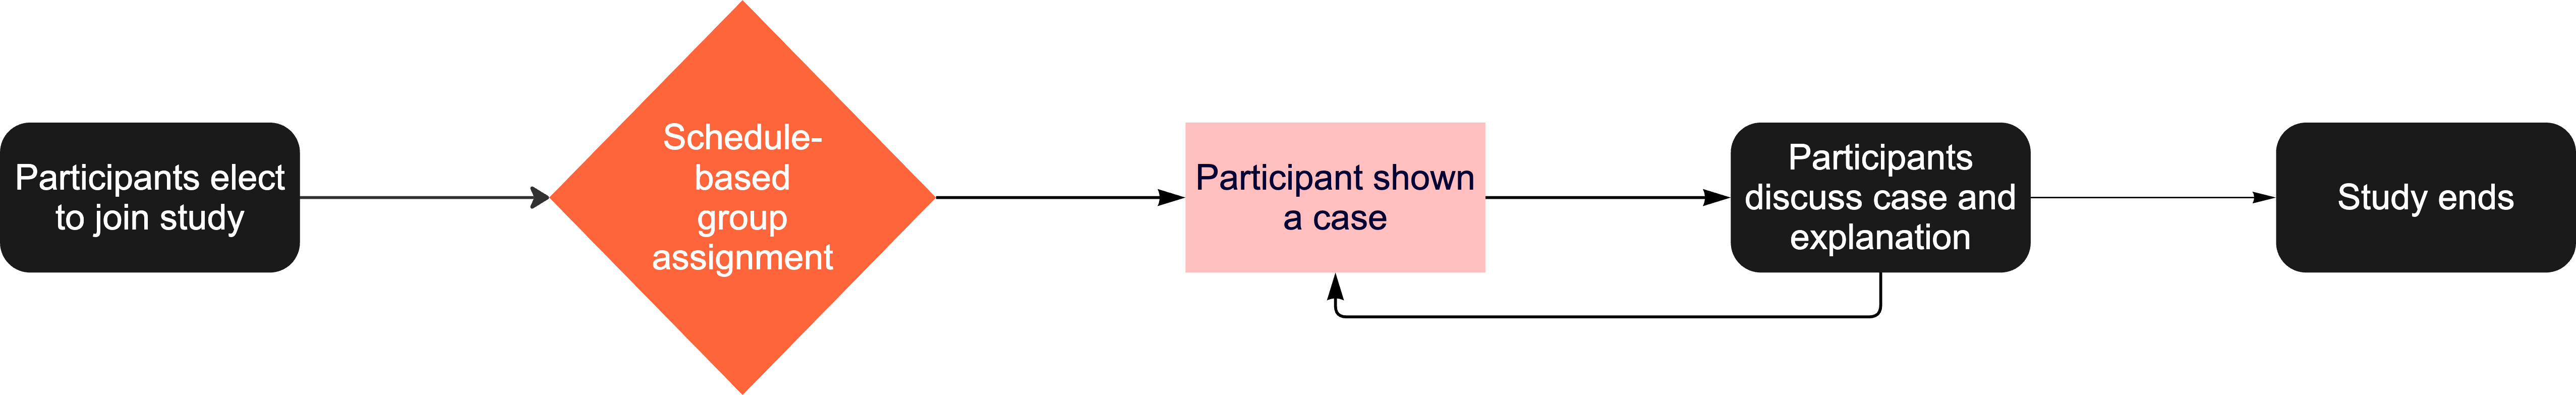
\includegraphics[width=.9\textwidth]{xai/case_flowchart.png}
    \caption{Each workshop consists of a series of cases relating to a past application decision that was flagged by program reviewers. In each case, participants are shown slides like in Figure \ref{fig:sample_case} and are asked to analyse the algorithm itself and whether the case warrants changes to the algorithm in future years.}
    \label{fig:case_flowchart}
\end{figure}

Both workshops followed an identical protocol. The flow of these workshops is shown in Figure \ref{fig:case_flowchart}, and more detail on the protocol followed can be found in Appendix \ref{app:xaiprotocol}.

In each workshop, participants discussed a number of cases, each examining a (possibly successful) applicant from a past application cycle who was flagged by program reviewers for having perplexing algorithm scores relative to other known information. In each case, participants are asked to use visual, SHAP-based explanations to first understand why program reviewers found these cases worth noting, then to explore why program reviewers gave the feedback they did and what caused the algorithm's perplexing outputs, and finally to opine on whether the case suggests that changes should be made to the algorithm (or to the selection process as a whole) for future years. The cases themselves have been redacted, as they contain sensitive information about program applicants, but a sample case can be seen in Figure \ref{fig:sample_case}.

In analysing our data, we follow \textcite{braun_using_2006}'s methodology for reflexive thematic analysis. 

\begin{figure}[htbp]
    \centering
    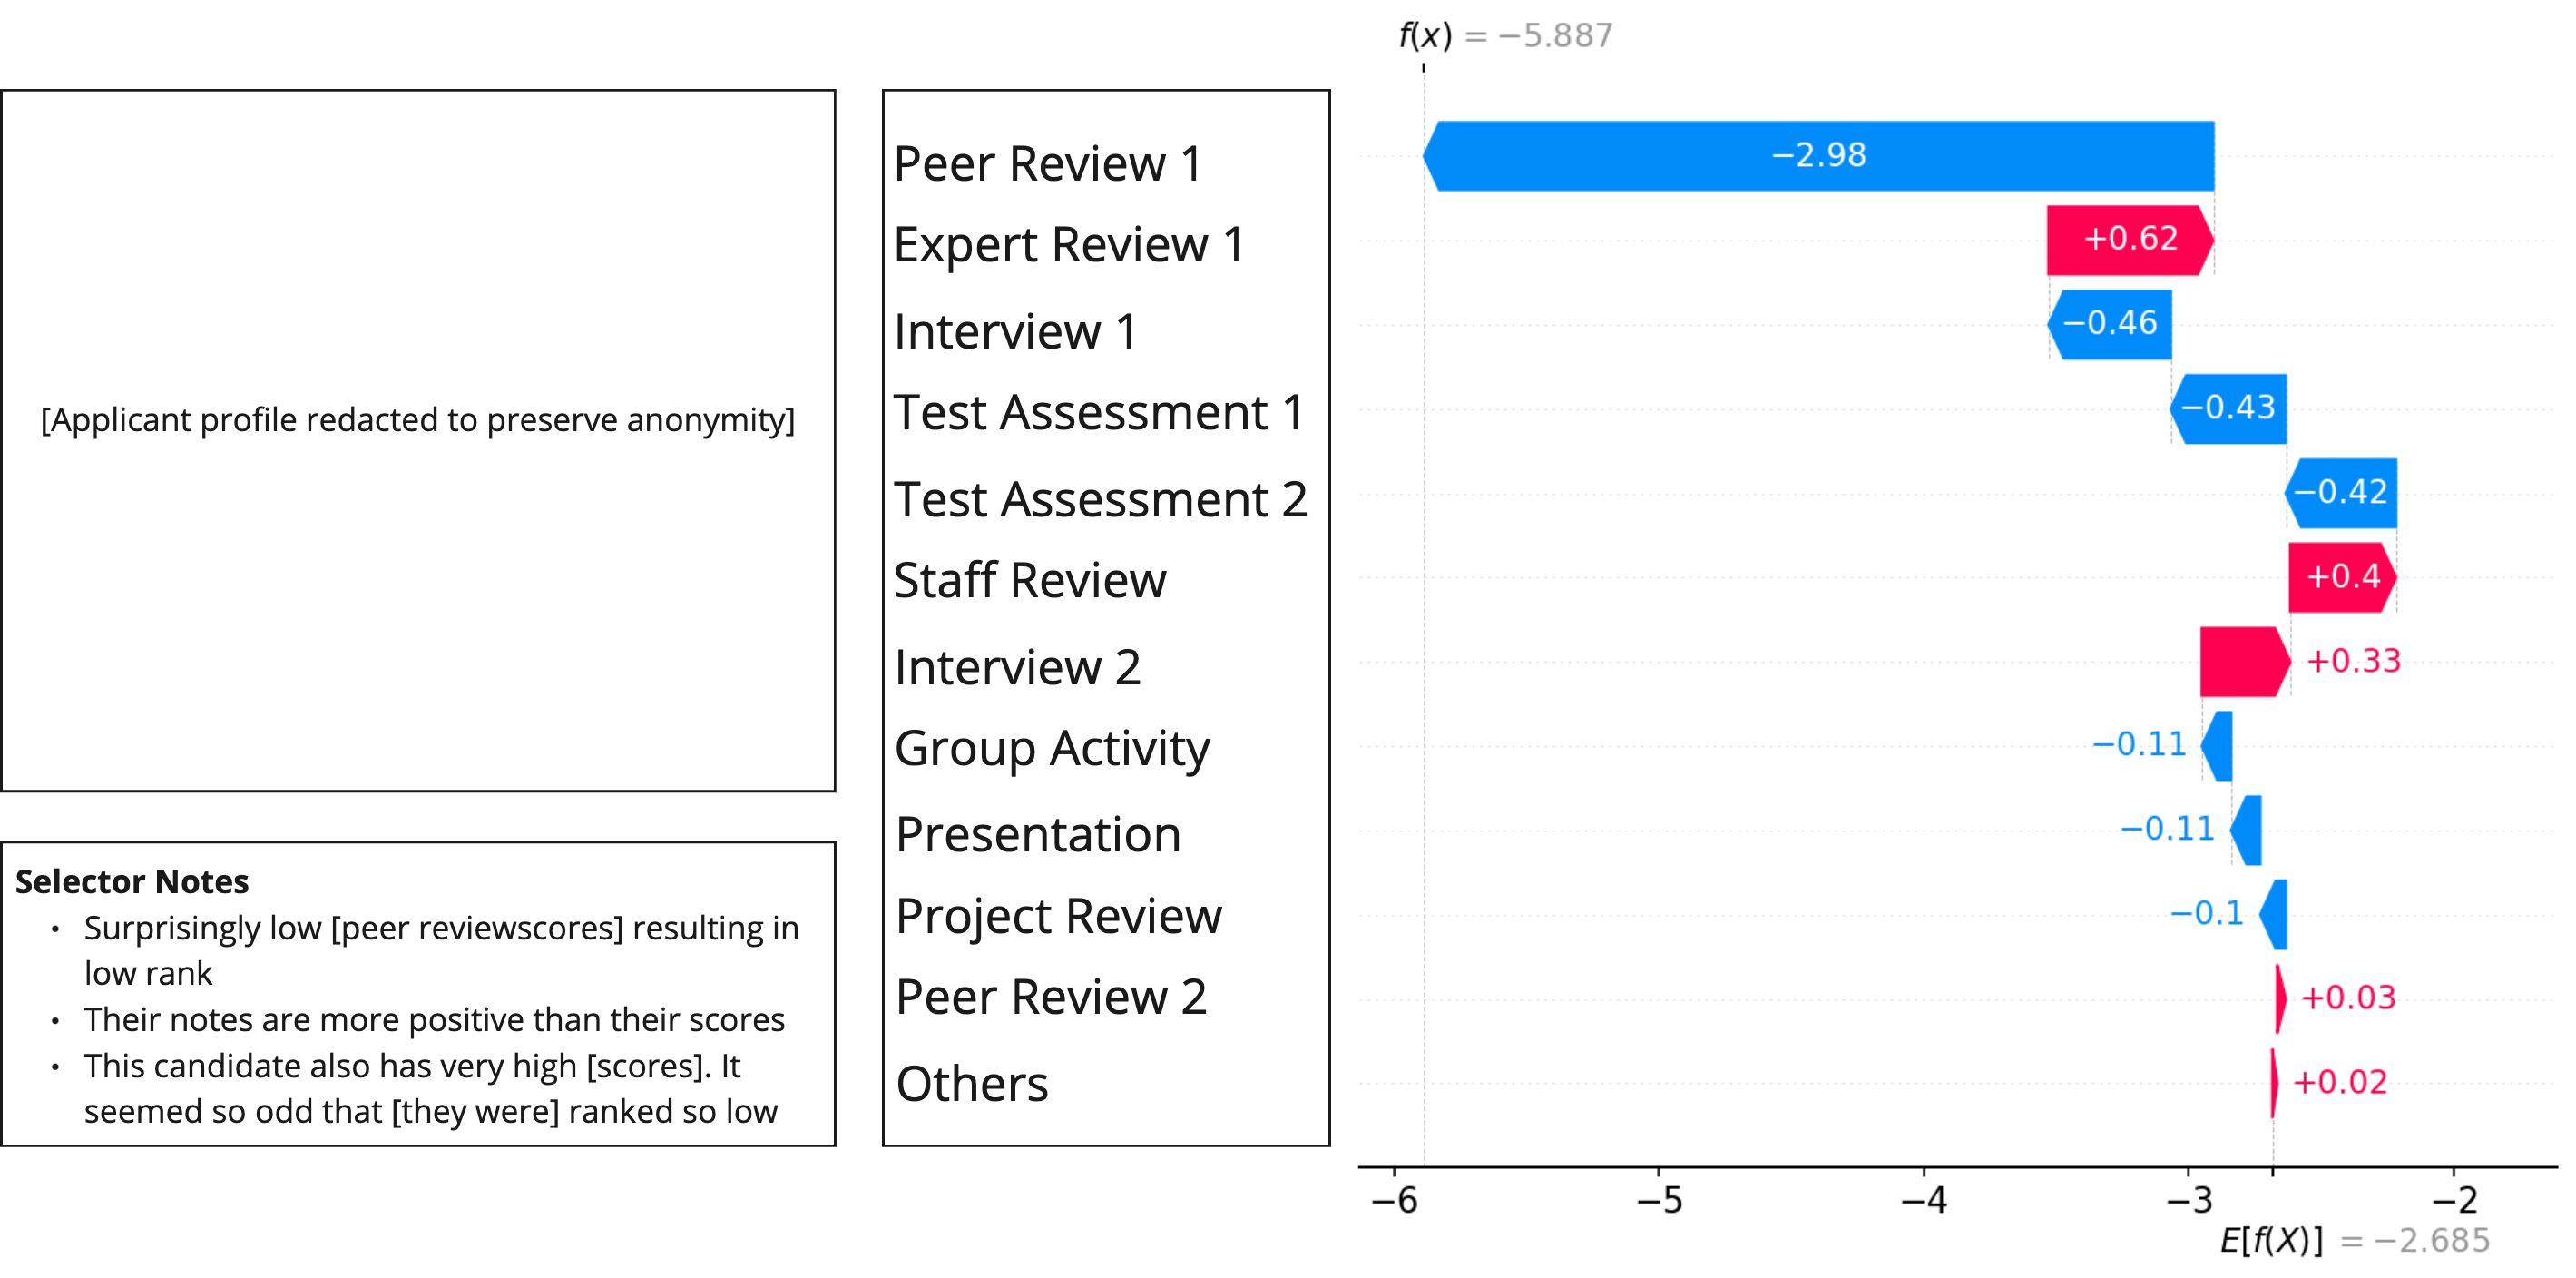
\includegraphics[width=.9\textwidth]{xai/sample_case.png}
    \caption{Each case explores one applicant from past years chosen by past program reviewers after being flagged as having perplexing algorithm scores. Each case contains the applicant's profile (overall algorithm scores alongside demographic information; the profile is redacted to preserve applicant anonymity), the program reviewers' comments, and the SHAP-based explanation (the score names are replaced with generic labels to preserve program anonymity).}
    \label{fig:sample_case}
    
\end{figure}

\subsection{Results}\label{sec:cs_results}
Our case study yielded two key themes. Firstly, SHAP Explanations yield useful \emph{ex-post} insights about feature importance. Second, even though SHAP yields useful information, the accessibility of such information depends on careful presentation. We now cover these in depth.

\subsubsection{Ex-Post Insights on Important Features}
In both groups, several useful insights emerged due to the SHAP visualisations. For example, the relationships between scores and contextual factors (e.g., markers of applicants' socioeconomic status) revealed that context plays little to no role in scoring; despite this, an applicant's context has a strong impact on how selection practitioners read scores. E.g., an applicant with high test scores from a poor region of Kenya is more impressive than one with high test scores from a rich part of the United Kingdom. When discussing one applicant who was selected, but had particularly low algorithmic scores, one participant said: ``This is one of the candidates that... [was from a] different country and [had] very low income'' (G1). Such cases raise difficult questions about fairness, including whether markers of disadvantage should be factored into decision-making, or if decision-makers should focus only on `task-relevant' factors \cite{dwork_fairness_2012}. If algorithms aren't taking into account such information, we are all but guaranteed to find discrepancies between algorithmically-driven selections and human-made ones.

It was also remarked on that scores calculated based on the feedback of external experts often disagreed with scores calculated based on the feedback of program applicants. It was discovered here that, contrary to program expectations, the program's expert reviews appeared less prone to biases than the peer ones. For one applicant: ``There was a question about why his peer and expert review were so different...I think confirms that it's not actually that they were seeing dramatically different things...his peers were dinging him for not seeming like he needed the award'' (G1). For another: ``I think this applicant has been significantly brought down by peer reviews; [their] scores are substantially lower than those that were, perhaps, given to [another applicant]'' (G1).

Similarly, it was observed that, unlike project reviews, group activities, and test results, the best candidates don't appear to have particularly good interview scores: ``I'm seeing also quite a few top ranked candidates whose interview score was really low'' (G1). In some cases, this appeared to create a discrepancy between algorithmically generated overall scores and the participants' perceptions of the best candidates: ``[The applicant's] staff reviews imply that [they] should be top 30, and even if you factor in low interview scores...[they] are still pretty low on the algorithm score'' (G2).

\subsubsection{Presentation is Key}
Besides insights about the selection process, the workshops yielded direct feedback on how the presentation of SHAP explanations should be improved. One major point was that contextual factors describing an applicant were missing. One participant said, of the explanation: ``It doesn't give me the context'' (G1). Another from the same group said: ``But I think without the context, it's really hard to decipher what's going on here'' (G1). This could be interpreted as participants asking for supporting information. However, when the researchers read out the information in the explanation's caption, this cleared up the participant confusion: ``Yeah, that makes sense'' (G1). This suggests that, rather than needing more information, participants needed the information presented in a different way.

Several times, participants were unclear on the meaning of different aspects of explanations: ``Should I be alarmed and I see it going blue in the context of this? It's really hard for me to, if you threw this at me...to compare'' (G1). Participants asked for the more complicated information as a ``Pre-reading'' (G2), and asked for simpler information, I.e., ``Maybe just colour coding things that are positive in one colour and then things that are negative in the other colours'' (G2).

One request that several participants echoed was that axes be kept constant, even between different types of scores: ``It's also different scaling. So, that massive bar...does not mean the same thing as the massive bar meant last time'' (G2). Another solution suggested to a similar problem was the provision of benchmark information: ``Like, give me the benchmark for that'' (G1).

\subsection{Participatory Design Study Findings}\label{ssec:cs_discussion}
Exposure to SHAP explanations appears to have yielded useful insights when used as part of an \emph{ex-post} decision-making process. In particular, participants appeared to find SHAP explanations useful for indicating when information may have been over- or under-used in practitioners' holistic review and in the algorithm itself. In this context, where decisions about individuals have already been made, and the organisation is looking into how to go about selecting its next cohort, the possibility of unwarranted trust in a particular output is not a concern. Rather, these explanations can be regarded as probes, or provocations, helping decision makers hone in on particular cases that highlight potential areas for improvement in decision-making, whether through changes in the model itself, or changes in human evaluation processes (e.g., placing greater or lesser weight on certain features). Thus, we can conclude that SHAP explanations may be useful \emph{ex-post}, when trust in the primary output is not at issue. Interestingly, the wolf-husky example from \textcite{ribeiro_why_2016}'s original LIME proposal could be interpreted as being used in a similar way; using an explanation of an existing classification to guide changes in the model in future (e.g. by adding an edge detection step prior to classification, to ignore snow in the background). In both cases, the explanation may reveal unwarranted reliance on (or lack of reliance on) a particular part of the feature space.

However, we also find that the SHAP-based waterfall explanations we provide, alone, lack the detail and presentation required. Practitioners desired additional context, additional modes of interaction with our explanatory materials, and points of comparison to clarify their investigation. This allays \textcite{miller_explainable_2023}'s concern that post-hoc xAI methods might discourage explainees from engaging deeply with the facts of the task. Rather, in this case, the explanations served as a platform for explainees to seek additional information to inform their decisions.

\section{Discussion, Limitations and Conclusion}
\subsection{Implications}
By delineating DSTs by the stage of decision they inform, we are able to answer the question ``should we use post-hoc xAI methods?'' separately for \emph{in-process} and \emph{ex-post} decisions. While we find them misleading, and thus dangerous, for \emph{in-process} decisions, Section \ref{ssec:os_discussion} indicates that these misleading tendencies are not limited to post-hoc xAI, and are rather a symptom of the practice of post-hoc justification more broadly. Furthermore, Section \ref{ssec:cs_discussion} indicates that certain \emph{ex-post} use cases do not necessarily require that explanations appropriately modulate trust. Thus, post-hoc xAI methods might still inform \emph{ex-post} decision-making (e.g., selection process refinement, evaluations of selector bias). This yields two direct implications for the xAI field:

\begin{enumerate}
    \item While we reiterate caution around post-hoc justification of model outputs \cite{miller_explainable_2023, Lipton, bansal_does_2021, ford_play_2020, jacobs_how_2021}, we extend this caution from xAI methods to any form of post-hoc justification.
    \item We qualify this caution in its application to \emph{ex-post} decision-making. We encourage a field that has, in large part, moved on from post-hoc notions of interpretability \cite{kumar_problems_2020,barocas_hidden_2020,Lipton,karimi_algorithmic_2021} to engage with and identify \emph{ex-post} applications for these tools.
\end{enumerate}

\subsection{The Anchor Problem}\label{ssec:anchor_problem}
Suppose a farmer sees what they believe to be a sheep on a hill, and states ``there is a sheep on that hill''. Now, suppose this farmer is in fact seeing a cleverly-disguised goat, but that there is also a sheep on the hill, only invisible to the farmer. In this case, the farmer has a true belief (``there is a sheep on that hill''), and has justification for it (the goat), but the justification is unrelated to the truth of the belief. In a seminal paper on Epistemology, \textcite{Gettier_1963} discusses this class of problem, now called the `Gettier Problems'., and maintains that, despite the truth of the farmer's belief, that farmer does not have knowledge. In keeping with this tradition, \textcite{Cabitza_Fregosi_Campagner_Natali_2024} argue that, if an explainee is presented with a trust-inducing misleading explanation, even if that explanation induces trust in a correct output, then the induced trust is misplaced.

In Section \ref{ssec:os_discussion}, we present what we believe is the most likely explanation for why Anchor explanations do not induce unwarranted trust: unlike SHAP and Confidence, these explanations might reveal concerns in the underlying model's local behaviour. However, other explanations exist. \textcite{miller_explanation_2017} describes desiderata that make explanations well-suited to most explainees: explanations should be contrastive, counterfactual, selective, and social. While Anchor explanations are not social, they are contrastive, counterfactual, and social. However, it may be that these explanations' beneficial effects on trust stem not from an ability to reveal concerns in the underlying model, but rather from subjective desiderata. In this case, Anchor might still mislead \cite{Lipton}.

\subsection{Limitations and Future Work}
One core limitation of our work relates to the choice of tasks. While \emph{Salary}, \emph{Credit}, and \emph{Refinement} are closely related tasks, the distinction between \emph{in-process} and \emph{ex-post} decisions may be complicated by other distinctions between the three tasks. Future work should investigate the this distinction in other contexts.

Another major limitation of our work stems from Section \ref{ssec:anchor_problem}'s Anchor problem. We recognise here that, though Sections \ref{ssec:history} and \ref{ssec:os_discussion} give a compelling theory for the surprising results surrounding Anchor explanations, we do not investigate here why Anchor explanations do not induce unwarranted trust. We expect future work will examine this.

Finally, differences between the personalities of our online study and participatory design participants may limit the external validity of our results. Similarly, though we choose popular post-hoc xAI methods \cite{barocas_hidden_2020,kumar_problems_2020,weerts_human-grounded_2019,ribeiro_nothing_2016}, our choice of SHAP and Anchor limits applicability to other methods.

\subsection{Conclusion}
\textcite{miller_explainable_2023} likens explanations provided by SHAP and related explanation systems to ``Bluster'', a hypothetical person that always gives a recommendation, even when unsure, and does their best to justify this. They note that, in the context of decision support, such a person is less valuable than ``Prudence'', who asks the decision-maker's opinion first then provides feedback, as Bluster risks discouraging explainee engagement with the decision. Here, we draw a distinction between \emph{in-process} and \emph{ex-post} \emph{decision stages}. We conclude that, while \textcite{miller_explainable_2023}'s conclusion applies straightforwardly to the \emph{in-process} stage, post-hoc xAI might still drive engagement and inform \emph{ex-post} decisions, and urge that more be done to identify and apply post-hoc xAI where it is useful. This chapter both hints at the significance of the distinction between \emph{in-process} and \emph{ex-post} decisions and hints towards the question: might other DSTs be more useful \emph{in-process}?

% \begin{savequote}[8cm]
% Alles Gescheite ist schon gedacht worden.\\
% Man muss nur versuchen, es noch einmal zu denken.

% All intelligent thoughts have already been thought;\\
% what is necessary is only to try to think them again.
%   \qauthor{--- Johann Wolfgang von Goethe \cite{von_goethe_wilhelm_1829}}
% \end{savequote}

\chapter{\label{ch:genai}What Are Generative AI Detectors Good For? Evaluating and Implementing with the Decision Matrix}

\minitoc

\section{Introduction}\label{sec:genaiintro}
Since \textcite{ashish_vaswani_attention_2017} introduced transformer architecture, AI has made rapid progress. More recently, large language models (LLMs) like BERT and GPT3 have demonstrated the ability to generate human-like text \cite{jacob_devlin_bert_2018,brown_language_2020}. The releases of GPT3.5 and GPT4o have made these models more powerful and ubiquitous, and students are increasingly using them to write essays \cite{openai_gpt-4_2023,dehouche_plagiarism_2021}. This has raised concerns about plagiarism, and while many generative AI (genAI)-users are caught by detectors, these detectors often fall short of their goal \cite{liang_gpt_2023,kalpesh_krishna_paraphrasing_2023,mitchell_detectgpt_2023,tharindu_kumarage_stylometric_2023,dehouche_plagiarism_2021}. Essay-writers' ability to use genAI has changed the role of essay-based teaching and evaluation, especially in competitive contexts like scholarship selection.

Many bodies of research seek to understand this new role. Among them, theoretical research attempts to determine what uses of genAI constitute plagiarism, or should otherwise be banned, and what uses do not \cite{yu_huang_reflection_2023,MikePerkins_JasperRoe_2023}. Meanwhile, practical research builds and evaluates genAI detectors to determine whether a ban on such use is enforceable \cite{mitchell_detectgpt_2023,tharindu_kumarage_stylometric_2023,kalpesh_krishna_paraphrasing_2023}. However, theoretical accounts focus primarily on what constitutes plagiarism, and detectors and their evaluations are often concerned with detecting said plagiarism under adversarial assumptions \cite{yu_huang_reflection_2023,kalpesh_krishna_paraphrasing_2023}. Work that does not overtly concern itself with plagiarism still grapples with issues of detecting and removing cohorts or passages, inadvertently viewing the problem through a plagiarism lens \cite{mitchell_detectgpt_2023,liang_gpt_2023}. This focus on plagiarism neglects other problems genAI has created for practitioners.

We address this here with Action Research (AR). We partner and ``research with'' \cite{bradbury_action_2003} an anonymous scholarship and talent investment organisation to understand the needs of their team of scholarship selection practitioners (N=8; excludes authors) with regards to categorising and interpreting application essays and undertake this research while supporting their 2022 and 2023 application cycles. We identify ``decision points'' when the program requires or desires to make a decision we might support with contextual information about genAI usage (see Table \ref{tab:decisions}). Through conversations with internal stakeholders \cite{Hayes_2011}, we identify two axes, `stage' and `stakes', on which these decisions exist \cite{braun_using_2006}; we use these axes to construct the Decision Matrix in Figure \ref{fig:decision_matrix}. We then evaluate three genAI detectors on these decisions.

AR revealed a number of decisions that selection practitioners desire to make surrounding genAI. Though the literature focuses on the decision of whether or not to disqualify applicants using genAI, our partner organisation dismissed this decision as irrelevant, as their application guidelines do not forbid the usage of genAI. Instead, the program expressed interest in decisions such as diligence, where the program provides information about genAI usage alongside other facts about the applicant to make a holistic decision about when and how to consider an applicant. We conceptualise these decisions in a Decision Matrix with axes relating to their `stage' (i.e., where does this fit in the selection process?) and `stakes' (i.e., what is the magnitude of the consequence of this decision?). We then identify the properties desired from detectors in order that they might support different decisions on different parts of our Matrix. In our evaluation of detectors for these decisions, we find that organisational needs are not met by current detectors, particularly with regards to in-process decision-making. Our results suggest that detectors can be useful in aggregate analyses to support ex-post decisions. As a case study, we use one of our detectors, GPTZero, to support two decisions: \emph{Partners} and \emph{Pipeline} (described in Table \ref{tab:decisions}). We demonstrate two applications of detectors to the support of ex-post decisions. The flow of this study can be seen in Figure \ref{fig:flow}.

At a high level, our paper has four major contributions:

\begin{enumerate}
    \item We identify decision points facing scholarship and talent investment programs regarding genAI through AR.
    \item We introduce the \emph{Decision Matrix} framework for categorising decisions and evaluating the decision support capabilities of genAI detectors.
    \item We apply this framework to two detectors, GPTZero and Originality.ai, on a scholarship program's 2022 and 2023 application data and determine their suitability for supporting specific decisions.
    \item As a case study, We use GPTZero to support two decision points, \emph{Partners} and \emph{Pipeline}, in our partner program's context.
\end{enumerate}

\section{Related Works}\label{sec:rw}
GenAI models have quickly surpassed what was previously thought possible with a natural language model \cite{brown_language_2020,chowdhery_palm_2022,openai_gpt-4_2023}. While their ability to respond with natural language is impressive, their use in academic writing raises questions; of particular note are those of fairness and integrity \cite{hu_challenges_2023}. In part due to these questions, there are many approaches to detecting AI usage, a vast majority of them commercial. Researchers have developed methods such as DetectGPT and stylometric detection, while commercial approaches include AI Writing Check, CatchGPT, Copyleaks, GPT Radar, GPTZero,  Turnitin, and Originality.ai \cite{mitchell_detectgpt_2023,kalpesh_krishna_paraphrasing_2023,tharindu_kumarage_stylometric_2023,gptzero_gptzero_2023,kirchner_new_2023}. These genAI detectors, much like genAI itself, have advanced rapidly in capability.

Many research institutions make their stances on pedagogical integrity clear. \textcite{h_holden_thorp_chatgpt_2023}, in an editorial from \emph{Science}, declares that ``the word `original' is enough to signal that text written by ChatGPT is not acceptable: It is, after all, plagiarized from ChatGPT''. The journal adopts a policy that: ``text generated by ChatGPT (or any other AI tools) cannot be used in the work, nor can figures, images, or graphics be the products of such tools'' \cite{h_holden_thorp_chatgpt_2023}. However, while research institutions face pressure to publish universal guidelines, researchers themselves are free to debate the theoretical and ethical implications of genAI usage \cite{lav_r_varshney_limits_2020,h_holden_thorp_chatgpt_2023,yu_huang_reflection_2023,weber-wulff_testing_2023,otterbacher_why_2023}. \textcite{yu_huang_reflection_2023} argues that these guidelines emerge as a result of pressure placed on organisations, and that, in the pursuit of academic integrity, these institutions hamper learning. A better system would encourage use of these new technologies and instead make appropriate adjustments to teaching methods and examination standards 
\cite{yu_huang_reflection_2023}. 

While the complete ban of genAI systems is perhaps disagreeable and unrealistic, it is at least clear. \textcite{MikePerkins_JasperRoe_2023} point out a problematic lack of clarity in policies that allow genAI for some uses, but not others. Under many of these guidelines, detection of genAI is not sufficient to determine whether program policy has been violated, as the nature of the usage of genAI must be compared to the program guidelines (e.g., if a line or paragraph is rewritten by a genAI, is this a form of writing, or editing?). \textcite{MikePerkins_JasperRoe_2023} do not encourage bans of genAI usage, instead arguing the virtues of ``integrating technology, education, policy reform, and assessment restructuring''.

Despite these urgings, the field remains preoccupied with the question of detecting AI-based plagiarism. Many papers have undertaken the task of determining whether genAI detectors can help censure writers who use AI. Some studies conclude that detection algorithms can be effective across a variety of simple detection tasks \cite{dugan_raid_2024,weber-wulff_testing_2023,tharindu_kumarage_stylometric_2023,elkhatat_evaluating_2023,mitchell_detectgpt_2023}. Other evaluations find that, for more complicated tasks such as detecting paraphrased AI-generated text, these detectors perform less well \cite{kalpesh_krishna_paraphrasing_2023}. Ostensibly unrelated to plagiarism, researchers are beginning to evaluate potential implications of using imperfect AI detectors \cite{liang_gpt_2023} or the implications of genAI for content creation \cite{kalpesh_krishna_paraphrasing_2023}. For example, comparing detectors' False Positive Rates (FPRs) for genuinely human-generated essays by from a US-based essay competition ($N = 88$) against those from Chinese English-language test takers ($N = 91$), \textcite{liang_gpt_2023} conclude AI detectors are biased against non-native English writers. Even still, these works concern themselves primarily with the question of whether a single essay includes any AI-written content; in adopting this viewpoint, they ascribe value to this individual-level determination, inadvertently viewing this problem through the lens of plagiarism.

Though the problem of detecting AI-written plagiarism is interesting, it is only one of the many problems practitioners evaluating essays are faced with. While theoretical work explores the implications of these other problems \cite{otterbacher_why_2023,yu_huang_reflection_2023}, practical work often overlooks practitioners' real and present need for solutions.

\begin{figure}[htbp]
  \centering
  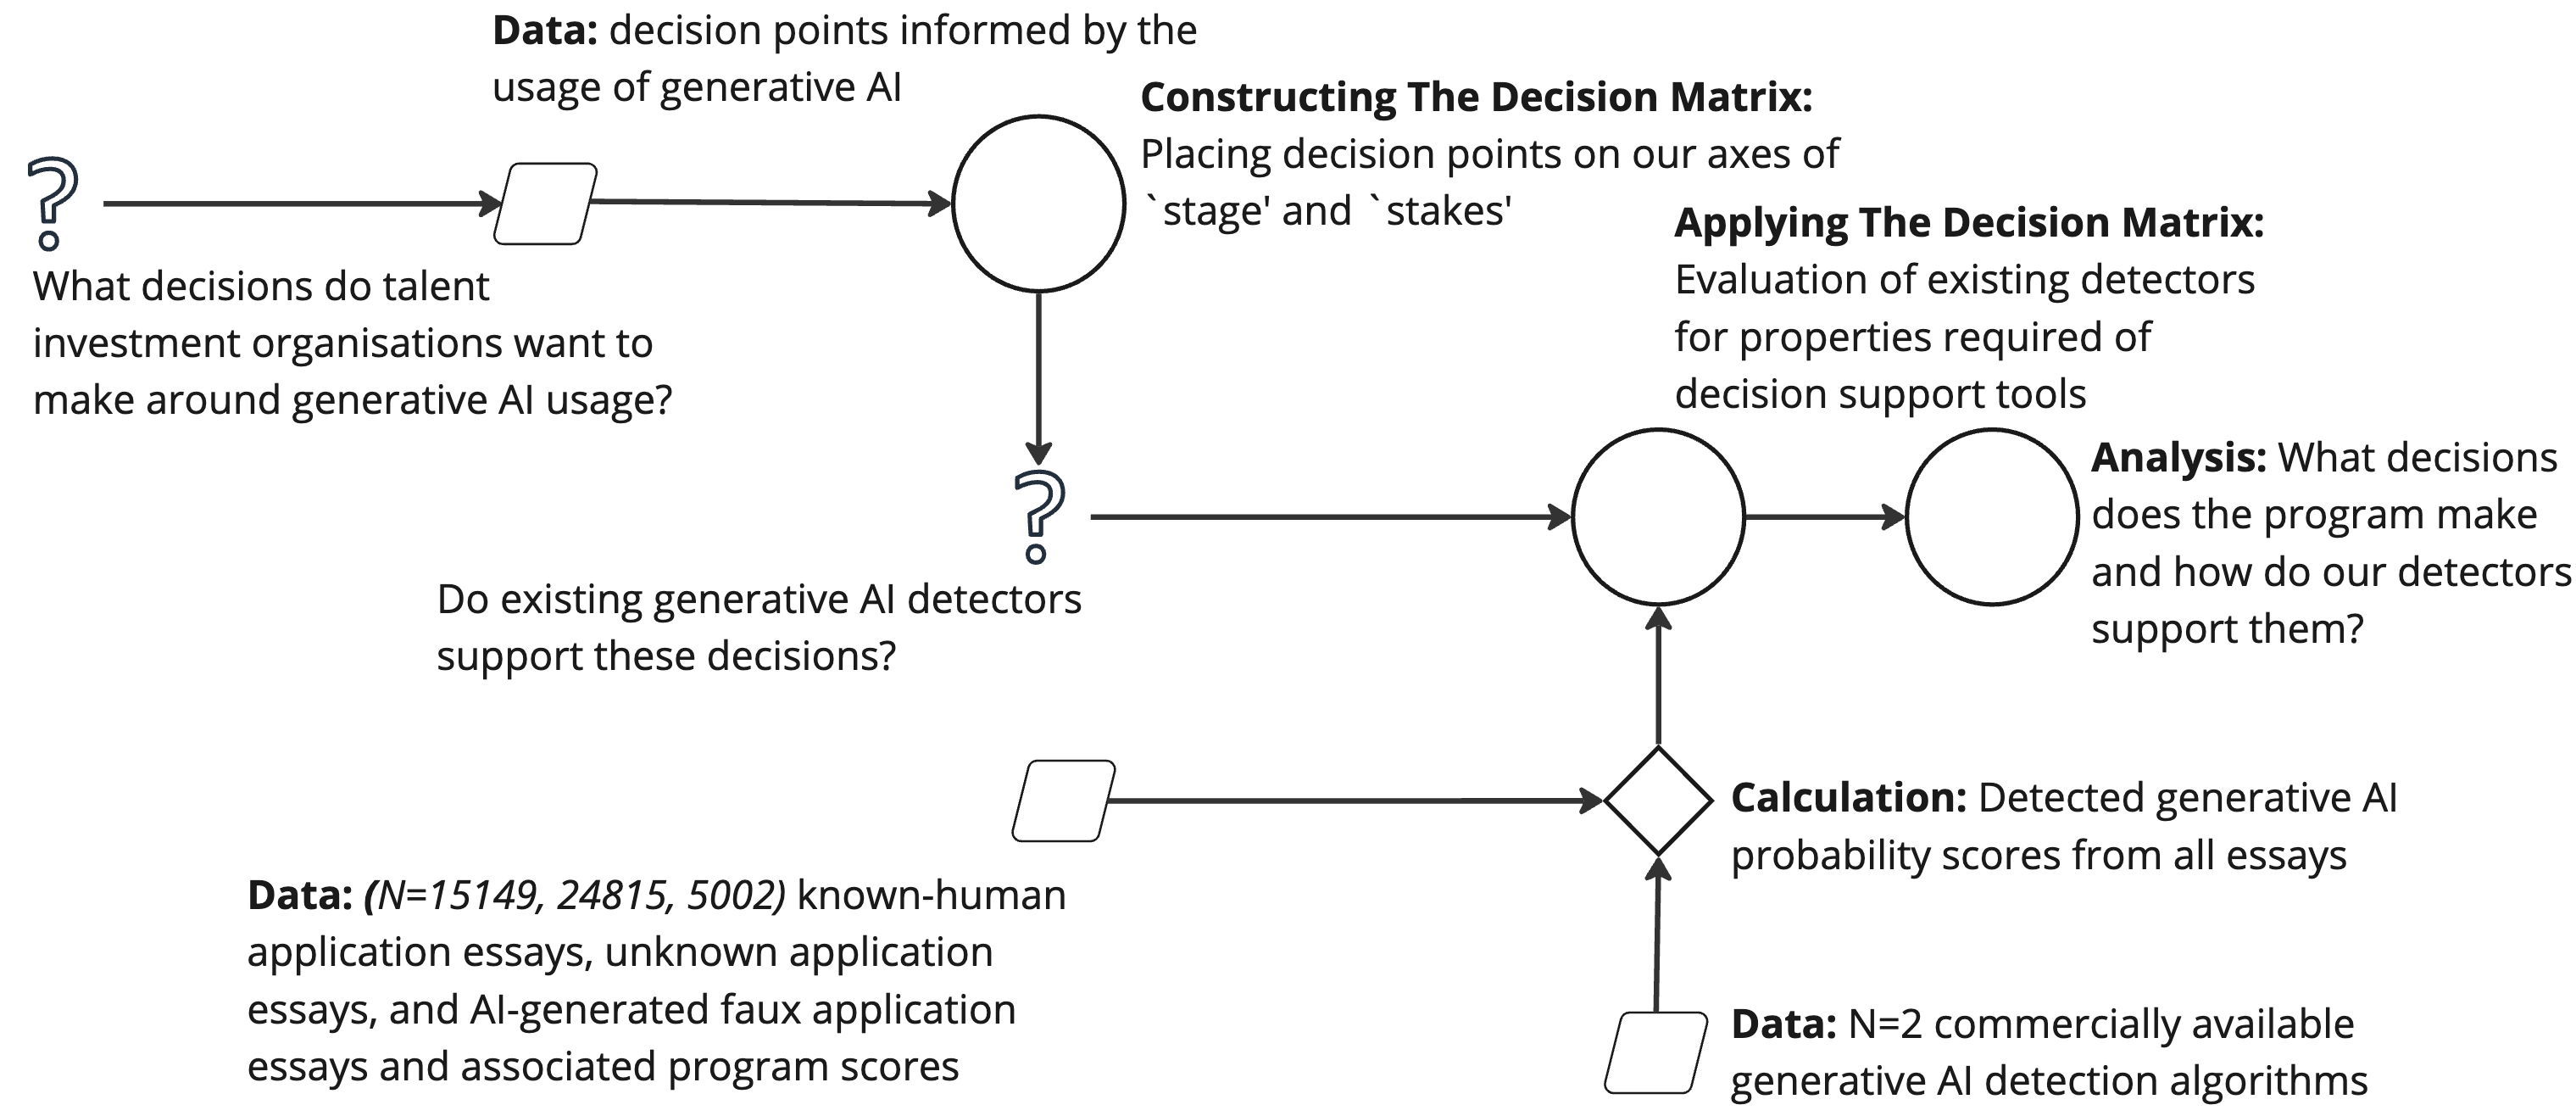
\includegraphics[width=\textwidth]{genai/study_flow.png}
  \caption{This figure describes the flow of our research.}
  \label{fig:flow}
\end{figure}

\section{Methodology and Action Research}\label{sec:embedded}
\subsection{What is Action Research?}\label{ssec:par}
Action Research (AR) is a research philosophy that emphasises ``research with, rather than on, people'' \cite{bradbury_action_2003}. Rather than one specific method, AR is best seen as a collection of related methods all embodying this ethos, usually with the goal of producing research contributions useful to the target group of people \cite{lu_organizing_2023}. Among these are semiotic inspection \cite{DeSouza_Leitão_2009,Alvarado_Waern_2018} and participatory design  (PD) \cite{braun_using_2006,Griffiths_Johnson_Hartley_2007,blythe2014research,Knapp_Zeratzky_Kowitz_2016}. AR is most often used in the context of social work, but can be applied across a variety of fields \cite{dombrowski_social_2016,lu_organizing_2023}. 

In education, AR is often used in a classroom setting \cite{Mertler_2019}. \textcite{venn-wycherley_realities_2024} argue that it is crucial in this setting to perform AR on both educators (teachers) and educatees (students), as failing to do so is liable to yield contributions useful to one group but not the other. While this holds for classroom settings, engagement across the stakeholder map is less feasible or desirable in scholarship selection. Unlike teacher and student, who share the common goal that the student learn, selector and applicant are at cross purposes: practitioners seek to choose the `best' cohort of applicants (although they often disagree on what constitutes `best'), while applicants seek to be included in the chosen cohort \cite{bergman2021seven}. Thus, when elucidating the interests and desires of one group, the other will merely act as noise. (E.g., applicants who use genAI to assist in writing their application will, of course, oppose using systems that monitor genAI usage to disqualify applicants.)

AR is comparatively new to HCI \cite{Hayes_2011,lu_organizing_2023}, but its methods and philosophies closely mirror longstanding pillars of HCI \cite{Hayes_2011}. Much like PD and other HCI methods, AR seeks to democratise the research and design processes; unlike PD, AR extends beyond building solutions democratically, and sees learning through action as the ultimate research contribution \cite{Hayes_2011}. For example, AR sees all parties Become: ``Co-investigators of, co-participants in, and co-subjects of...the project'' \cite{Hayes_2011}.  Thus, research questions are formulated by and with participants, actions and interventions are designed by and with participants, and results are found by and with participants \cite{Hayes_2011}.

\subsection{Our Action Research}
In many scholarship selection contexts, organisations typically select groups of talented young people based on applications consisting variously of: essays, videos, test scores, interviews, project results, group or individual activities, etc.. The organisation will begin by narrowing down the pool of candidates, often based primarily on test results, project results, or other easy-to-gather information. The organisation likely then compiles information from the application into short-form summaries of each applicant, complete with internally-generated scores, and often even a recommendation. This recommendation is then often reviewed by a selection committee, who craft a cohort from the recommended applicants.

We engage a scholarship and talent investment organisation in AR to investigate this selection context. In engaging this organisation in AR, several of the authors also functioned in supporting roles for the organisation's 2022 and 2023 selection cycles. In addition to working alongside the selection practitioners themselves, the authors were, at the time, a part of the scholarship organisation. Thus, throughout the paper, we refer to this organisation as our `partner organisation'. 

As with all AR, we first worked with participants (N=8; excludes authors) to identify research questions. We did this via a mixture of synchronous and asynchronous interactions. After this, we evaluated two genAI detectors, GPTZero and Originality.ai, according to our research questions. Finally, we implemented one genAI detector as an intervention. The flow of this study can be seen in Figure \ref{fig:flow}.

Before our study, we obtained consent from all 8 participants to be included. Applicant essay data was collected by our partner organisation, who obtained consent to use these essays (anonymously) for research purposes. Participants also gave consent to be recorded, and to have these recordings stored on a secure server. All recording, transcribing, and data analysis was conducted on secure servers. Ethics review was performed by University of Oxford's Central University Research Ethics Committee.

\subsection{Positionality}
Following \textcite{venn-wycherley_realities_2024}, we state researcher positionality here. The research team is comprised of five researchers split between the United States and United Kingdom; all researchers are men; four out of five researchers are ethnically White, while the fifth is South Asian; three researchers are affiliated with the University of Oxford and two are affiliated with Schmidt Futures.

\begin{table}[htbp]
  \centering
  \caption{Our partner program discussed a desire to make several decisions with regards to genAI. These decisions and the information desired to support them are detailed here. Though the program discussed disqualification, the program has no application guidelines surrounding the use of genAI and expressed no interest in disqualification. We include it here due to its ubiquity elsewhere in the literature \cite{liang_gpt_2023,mitchell_detectgpt_2023,tharindu_kumarage_stylometric_2023,kalpesh_krishna_paraphrasing_2023}.}
  \label{tab:decisions}
  \begin{tabular}{ p{0.2\linewidth}p{0.3\linewidth}p{0.5\linewidth}}
      \toprule
      Decision Point & Decision Description & Supporting Information \\
      \midrule
      \emph{Diligence} & The program makes holistic decisions about when and how to consider applicants. & Information about which essays (and which parts of essays) were written by genAI; information about whether the genAI-written passages are hallucinations. \\ 
      \emph{Partners} & The program must determine whether to continue channel partnerships, which encourage and support applicants. & Whether any channel partners' affiliated applicants use genAI disproportionately. \\
      \emph{Pipeline} & The program decides whether to modify their application material or process. & Information about usage of genAI throughout the application pipeline. \\
      \emph{Gameability} & The program decides how to modify their application material or process. & Information about the how AI-generated essays are scored under the current application process. \\
      \midrule
      \emph{Disqualification} & A program may decide to disqualify an applicant that violates their application guidelines. & Information about whether essays violate application guidelines around genAI usage. \\
      \bottomrule
  \end{tabular}
\end{table}


\section{Constructing the Decision Matrix}\label{ssec:poi}
We began from a starting point of ``What do we do about genAI?''. Literature about genAI elsewhere prompted early discussions to focus on: ``Can we determine whether an applicant used genAI to plagiarise?'' but quickly discarded this; the partner organisation had no application guidelines forbidding genAI usage, and hoped to accommodate ``innovative uses of this powerful technology'' in their selection process. From there, we quickly moved to ``What decisions do talent investment organisations want to make around generative AI usage?''. We then sought out other decisions the program wished to make in response to genAI. Ultimately, we identified the decision points in Table \ref{tab:decisions}; our final research question, then, is ``Do existing generative AI detectors support these decisions?''.

Notably, the decision to disqualify applicants for using genAI (\emph{Disqualification}) appears several times in the literature surrounding potential use cases for detectors \cite{gptzero_gptzero_2023,kalpesh_krishna_paraphrasing_2023}. Thus, despite our partner organisation's dismissal, we list it alongside the different decisions discussed in Table \ref{tab:decisions}.

\begin{figure}[htbp]
  \centering
  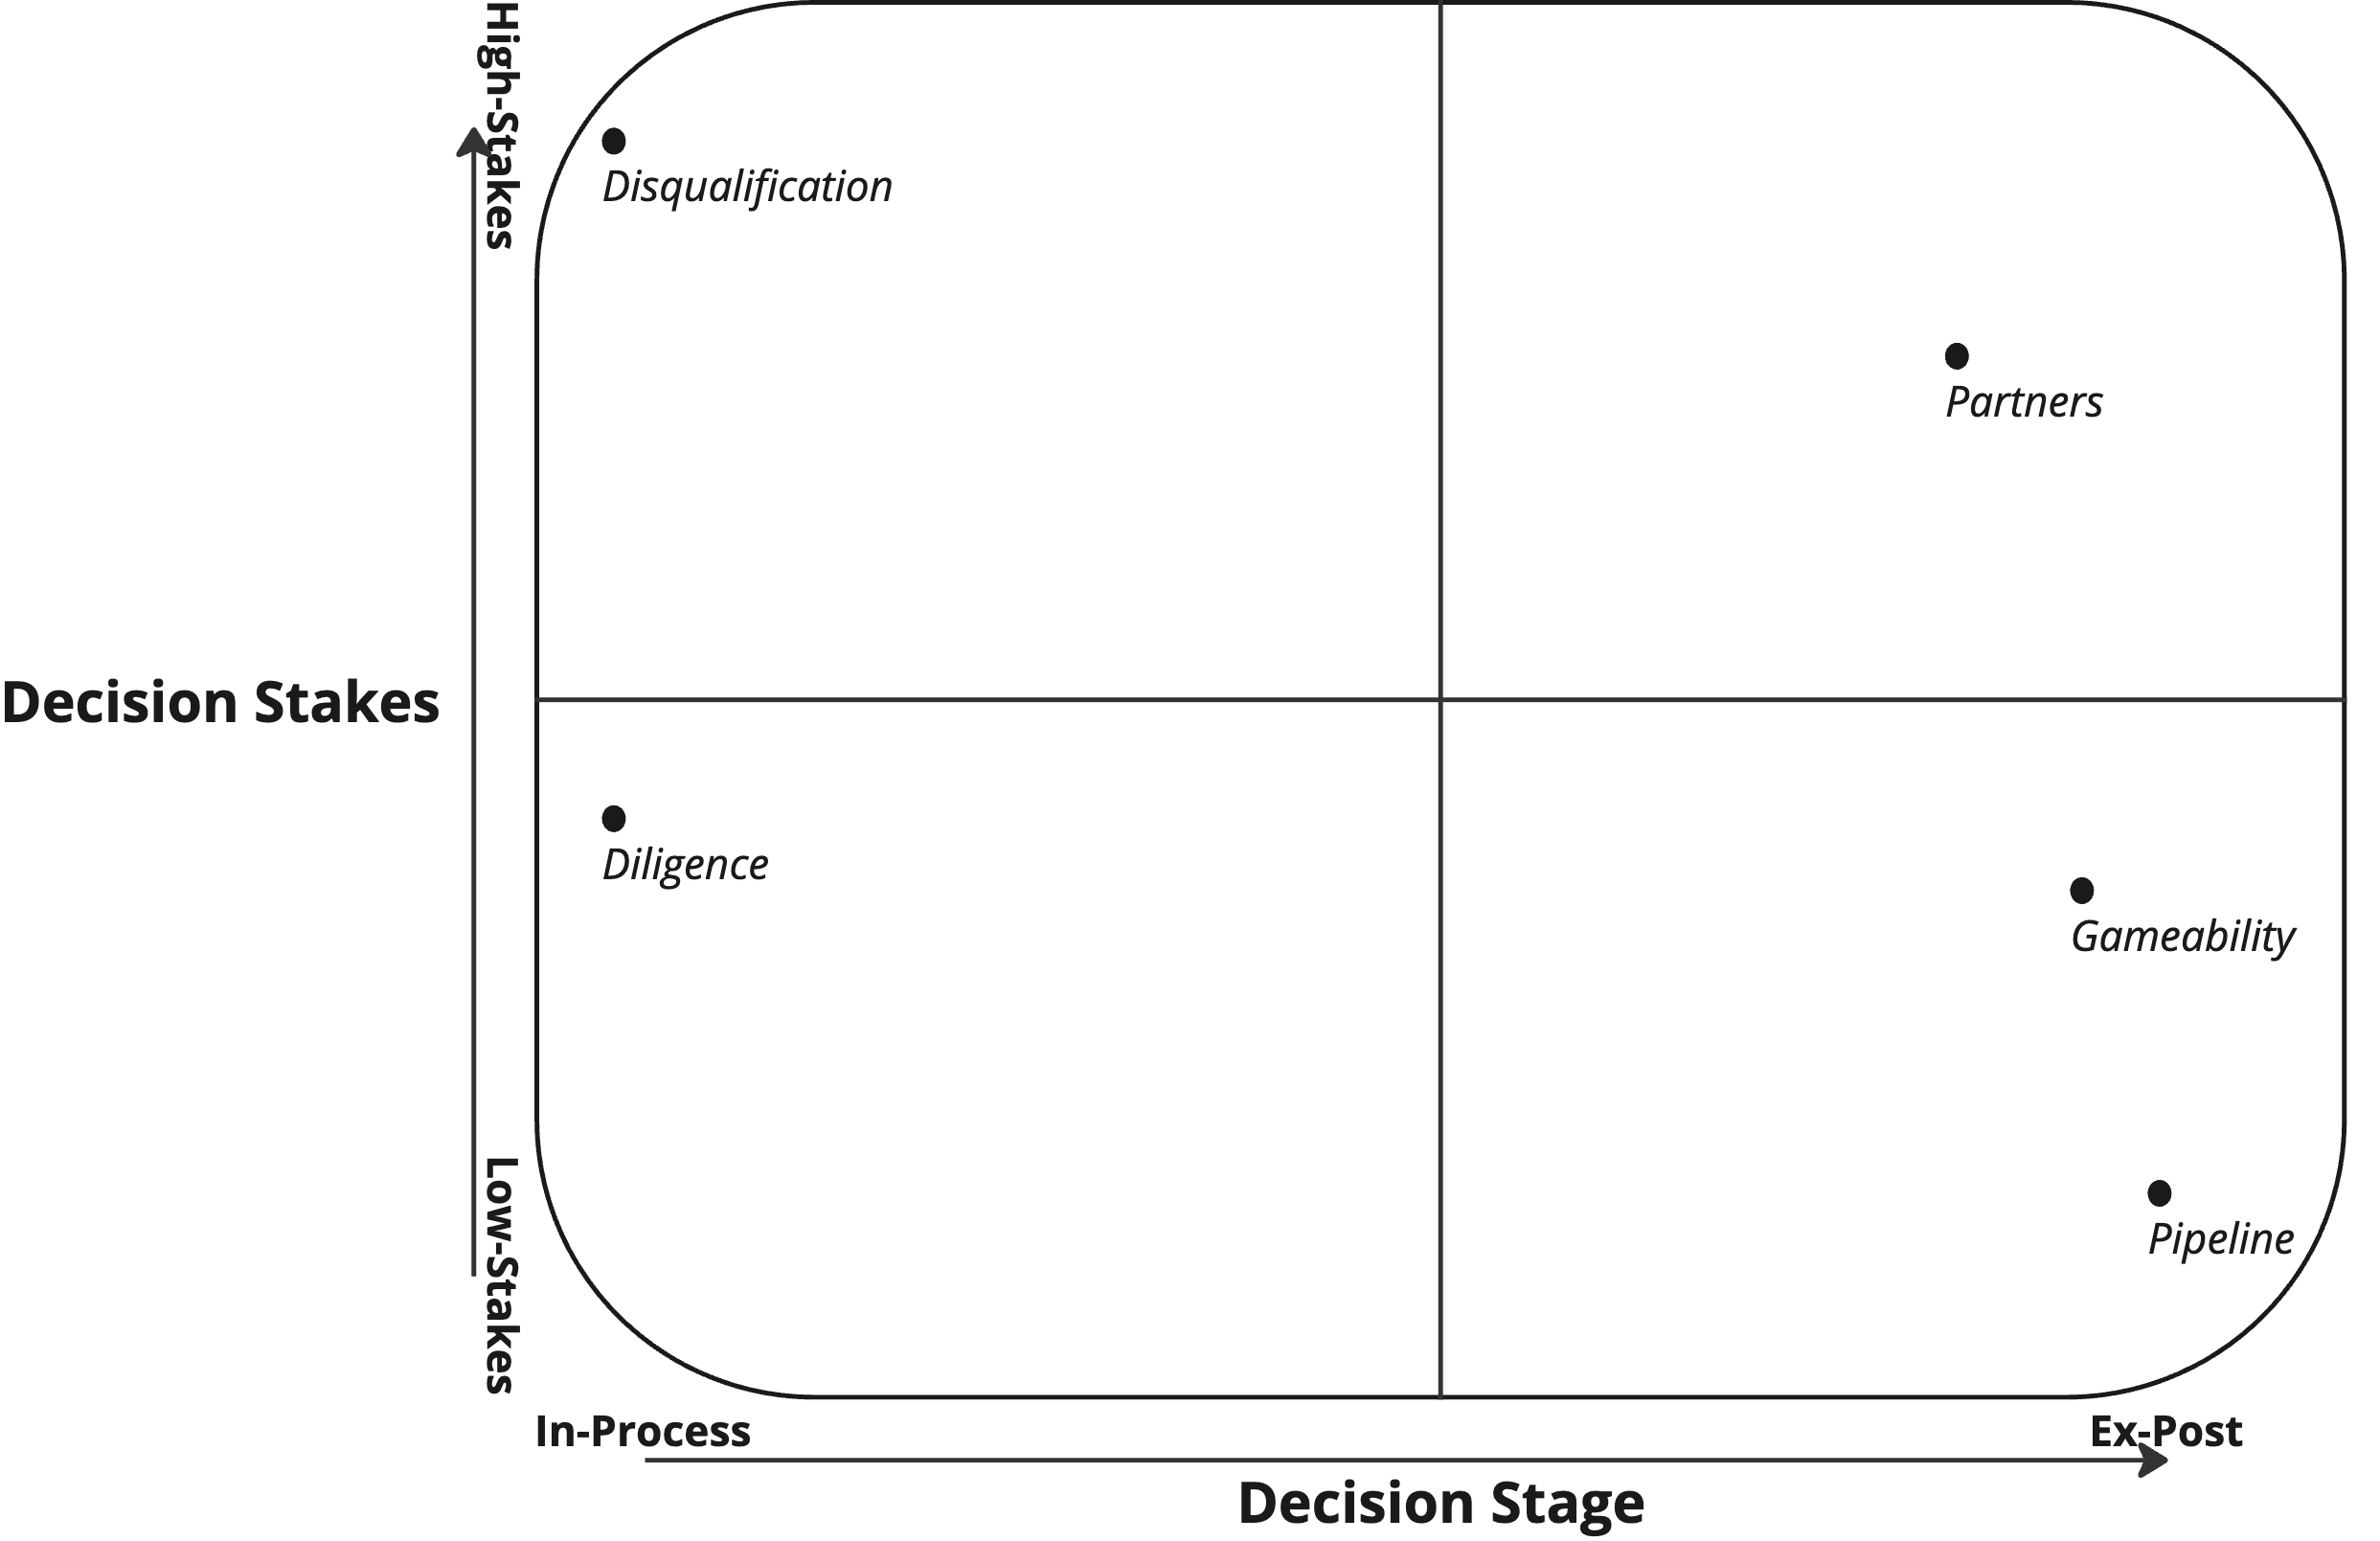
\includegraphics[width=0.8\textwidth]{genai/decision_matrix.png}
  \caption{This figure places the decisions from Table \ref{tab:decisions} on the Decision Matrix, with axes of `stage' and `stakes'.}
  \label{fig:decision_matrix}
\end{figure}

In conversation with practitioners in our partner program, we isolated two `axes' on which the decision points exist: stage and stakes. Decision stages vary from entirely in-process (`primary' decisions during the selection process) to entirely ex-post (`secondary' decisions about future selection processes). Meanwhile, decision stakes vary from very low (e.g., a due-diligence decision to investigate further) to very high (e.g., a decision to disqualify an applicant). Figure \ref{fig:decision_matrix} uses these axes to categorise the decisions in Table \ref{tab:decisions}.

We also work with practitioners to determine what type of properties a detection score should have to support each decision. For example, a disqualification decision may have stricter requirements than a diligence one. We lay out these desiderata on the same axes as Figure \ref{fig:decision_matrix} in Figure \ref{fig:desiderata_matrix}. 

\begin{figure}[htbp]
  \centering
  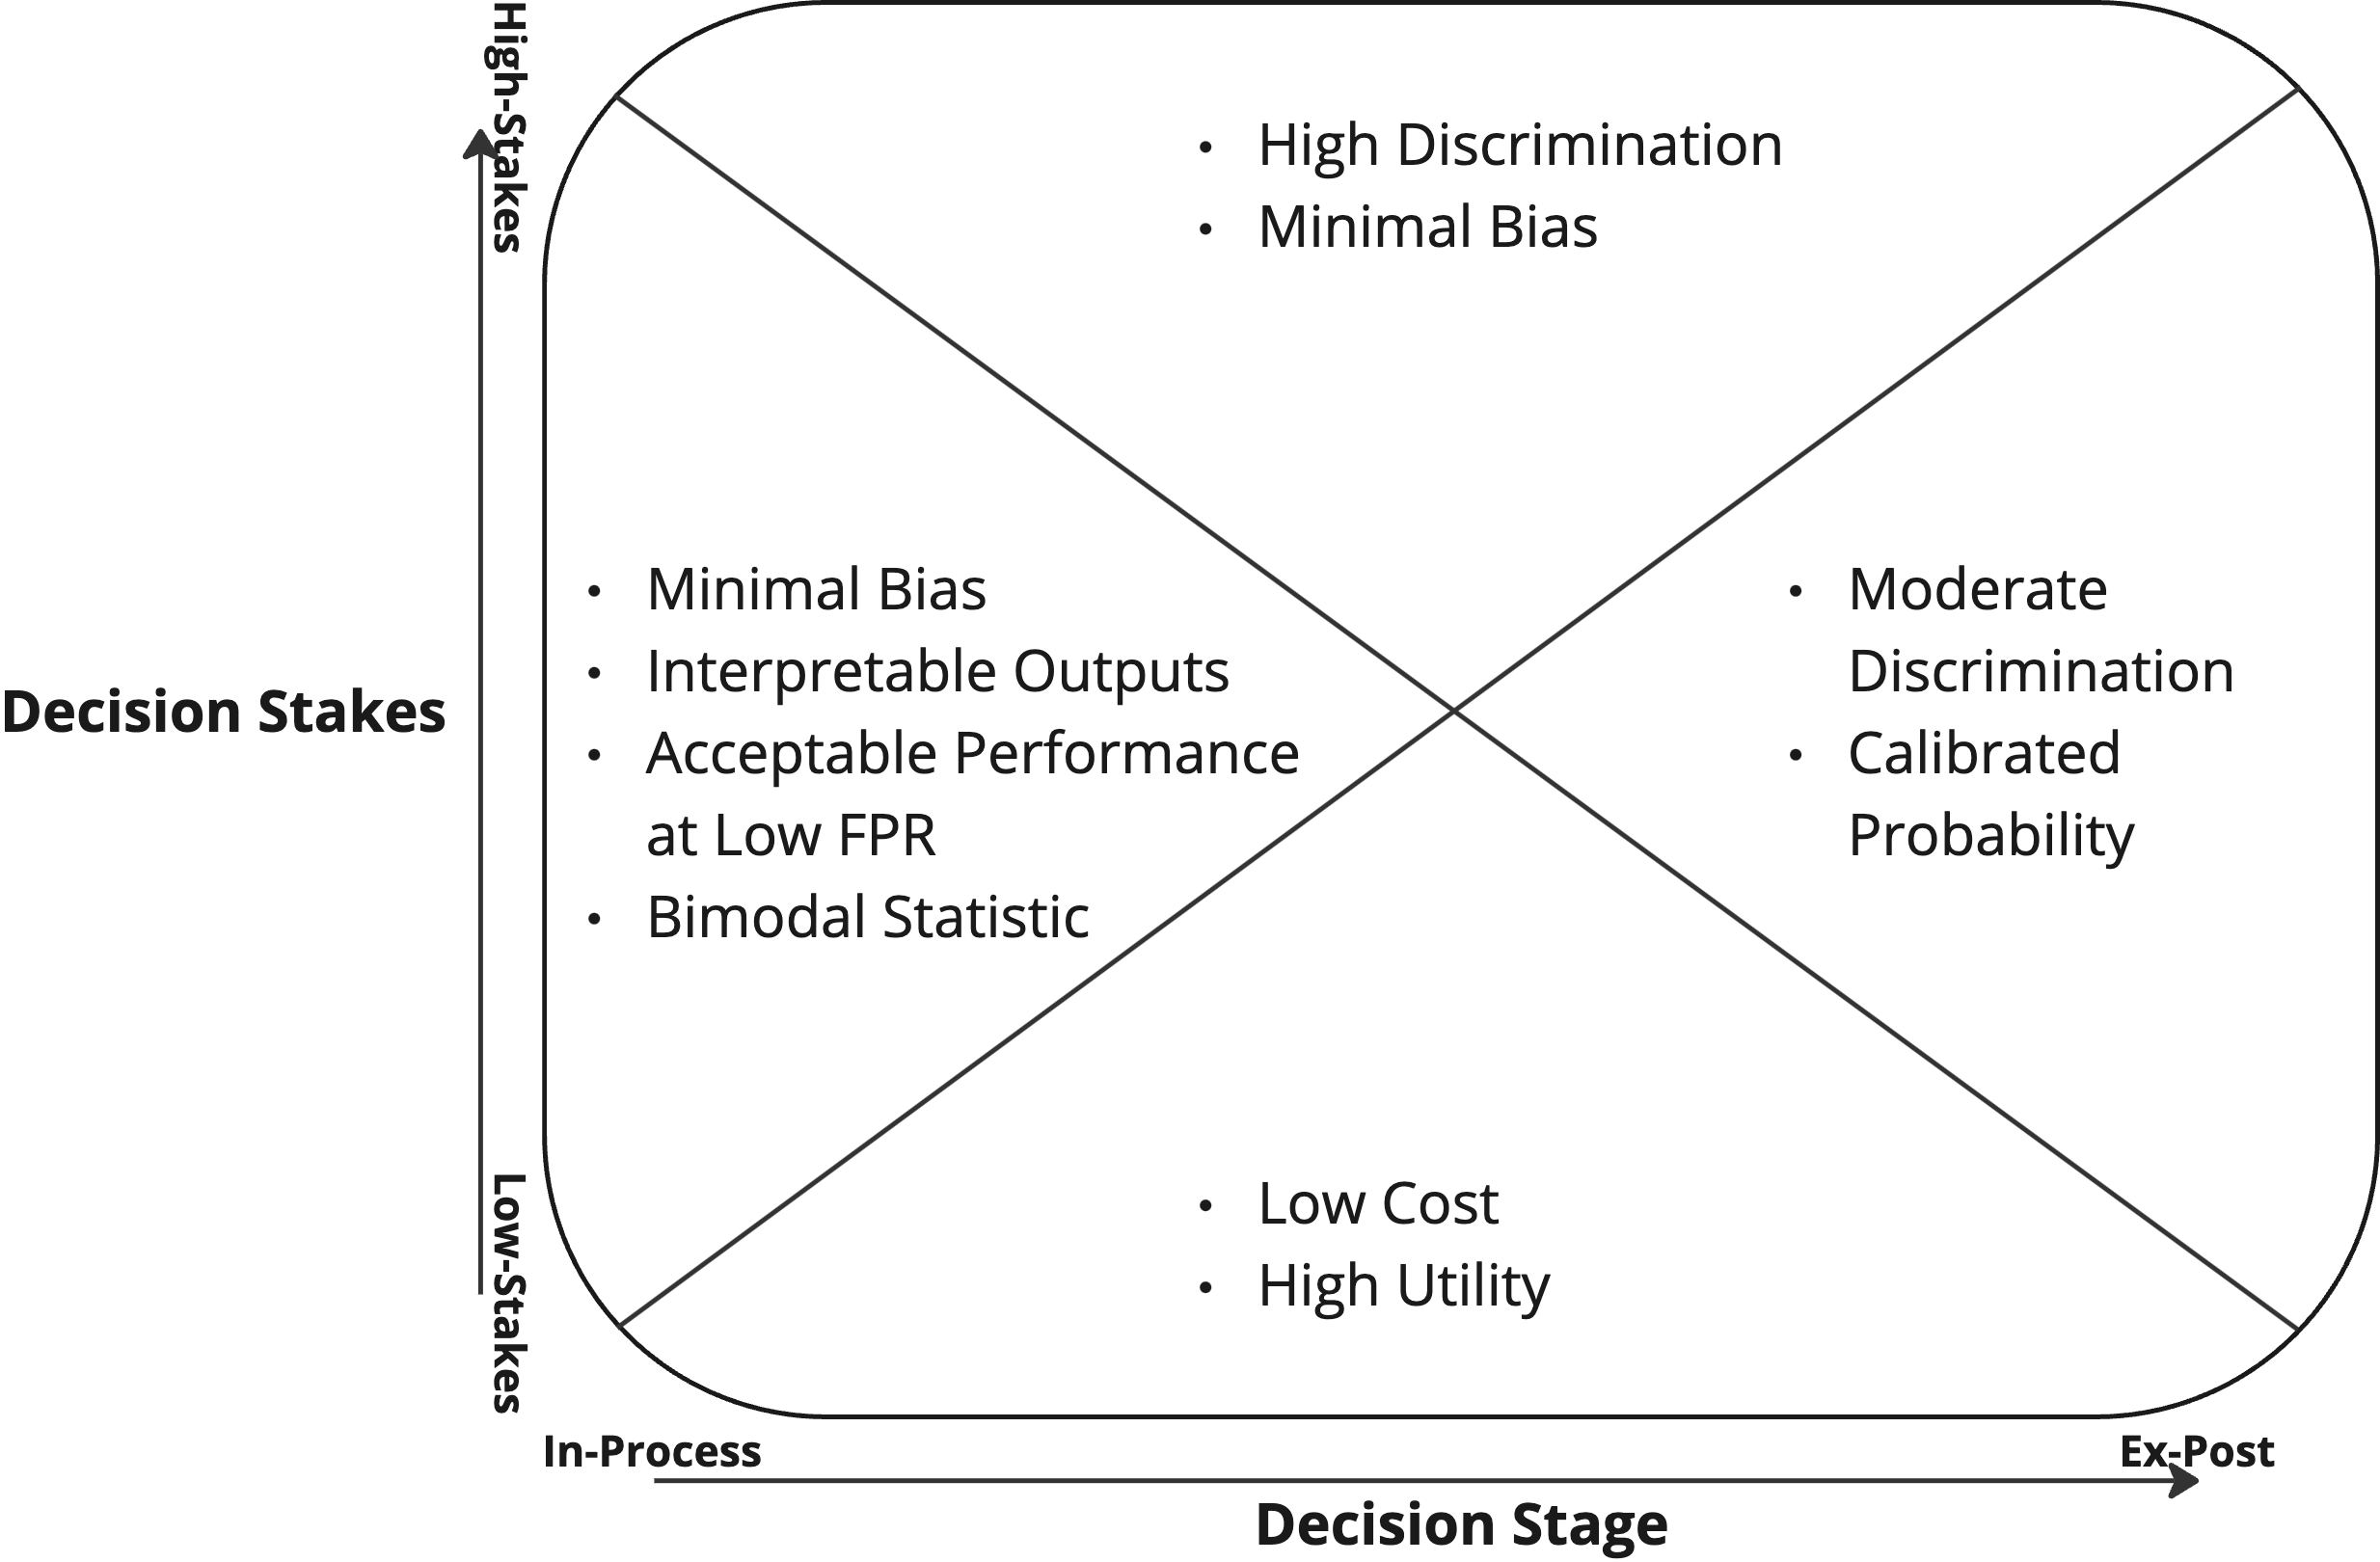
\includegraphics[width=0.8\textwidth]{genai/desiderata_matrix.png}
  \caption{This figure places uses our Decision Matrix to understand properties of genAI detectors required (or, in the case of low-stakes decisions, desired) to support each decision.}
  \label{fig:desiderata_matrix}
\end{figure}

\section{Applying the Decision Matrix}\label{sec:data}
\subsection{Evaluating for Decisions}
We seek to evaluate genAI detection software for its suitability in supporting decisions across the Decision Matrix in Figure \ref{fig:decision_matrix}. To do this, we first evaluate detectors on the properties outlined in Figure \ref{fig:desiderata_matrix}; if a detector has the properties outlined in both low-stakes and ex-post decisions, it is likely to be useful in supporting decisions from this quadrant. However, although our partner program indicated that these properties are necessary, we still seek to test their sufficiency. Thus, where the desiderata are satisfied, we apply the detectors to specific decisions from Figure \ref{fig:decision_matrix}. In particular, we select one decision from each quadrant (unless all detectors are deemed to lack the properties required for decision support in that quadrant). Finally, in case multiple detectors have sufficient properties, we compare detectors directly to make a recommendation about which method practitioners should use for these use cases.

\subsection{Data}
\subsubsection{Applicant Data}\label{sssec:applicant_data}
We use data from two of our partner program's application cycles, which we term Cycle 2022 and Cycle 2023.

Applications for Cycle 2022 were due in early 2022, well before ChatGPT's public release, so we assume that these submissions were written without the use of genAI \cite{openai_gpt-4_2023}. Applications for Cycle 2023 were due in early 2023, so genAI tools were widely available and AI detection tools were already emerging \cite{kirchner_new_2023,gptzero_gptzero_2023,liu_deid-gpt_2023}; we thus make no such assumption for these applications.\footnote{A number of avoidance detection strategies (e.g., paraphrasers) have been proven to severely hamper state-of-the-art detection \cite{kalpesh_krishna_paraphrasing_2023}. However, as of the 2023 deadline, the efficacy of these detection avoidance strategies was not well-known. Thus, we assume these strategies were not widely employed.}

\begin{table}[htbp]
    \centering
    \caption{This table shows the total number of submitted essays evaluated across years and demographic groups.}
    \label{tab:demo_counts}
    \begin{tabular}{ l r r }
        \toprule
        Demographic Group & 2022 Essays & 2023 Essays \\
        \midrule
        Male & $6,475$  & $11,080$ \\
        Female & $8,710$  & $13,380$ \\
        Other & $176$ & $355$ \\
        \midrule
        Caribbean & $128$ & $75$ \\
        East and Southeast Asia & $1,332$ & $395$ \\
        Core Anglosphere & $522$ & $1,865$ \\
        Eastern Europe / Central Asia & $85$ & $705$ \\
        South Asia & $2,130$ & $2,560$\\
        Latin America & $709$ & $2,855$ \\
        Middle East / North Africa & $1,363$ & $4,100$ \\
        Sub-Saharan Africa & $8,972$& $8,375$\\
        Western Europe & $59$ & $560$ \\
        Pacific Islands & $5$& $0$ \\
        \midrule
        Total & $15,149$ & $24,815$ \\
        \bottomrule
    \end{tabular}
\end{table}

Each applicant submitted essays in response to five prompts. These prompts are not described in more detail to preserve our partner organisation's anonymity. Applicants in both cycles provided information on their background, including gender identity and countries of citizenship. 

Applicants were asked their gender identity and given options including `male', `female', `non-binary', `other', and `prefer not to say'. The program uses all categories. However, the vast majority selected `male' or `female', so, in order to avoid spurious results from small samples, we group `non-binary' and `prefer not to say' under `other' for this analysis. 

Similarly, applicants reported their primary, secondary, and tertiary nationalities (where they exist). The program uses only primary nationalities in this context, and has, throughout the 2022 and 2023 application cycles, grouped applicants in various ways. The program uses the given `semi-regional' groupings to capture relevant similarities between nationalities (e.g., while `Core Anglosphere' is not a distinct geographic region, applicants from Core Anglosphere countries tend to speak English as their first language, come from similar school systems, and share similar facets of culture). These regional groupings are the program's. At the program's request, we do not share specific country-to-region codings.

Table \ref{tab:demo_counts} describes the analytic sample of essays by these demographic dimensions for each cycle. 

\subsubsection{Synthetic Data}\label{sssec:chatgpt}
To obtain a set of known AI-generated essays, we generate $5,002$ synthetic essays using OpenAI's ChatGPT API and Cycle 2022 prompts. These sit alongside our $15,149$ human-written, applicant-submitted Cycle 2022 essays and form our Cycle 2022 corpus. In contrast, our Cycle 2023 corpus consists entirely of applicant-submitted essays, though it is unknown how many of these are AI-generated. Our entire corpus is detailed in Table \ref{tab:cycle_counts}.

\begin{table}[htbp]
  \centering
  \caption{This table shows the total number of (submitted and generated) essays. The top row, Cycle 2022 submissions, is assumed to be human-written, as the Cycle 2022 submission deadline predates the release of ChatGPT. The second row lists essays generated by the authors in response to the Cycle 2022 prompts. The third row lists submitted essays of unknown providence from the 2023 application cycle.}
  \label{tab:cycle_counts}
  \begin{tabular}{ l r }
      \toprule
      Source  & Essays \\
      \midrule
      Cycle 2022 Submissions (Assumed Not AI) & $15,149$ \\
      ChatGPT Responses to Cycle 2022 Prompts & $5,002$ \\
      Cycle 2023 Submissions (Potentially AI) & $24,815$ \\
      \bottomrule
  \end{tabular}
\end{table}

All of our synthetic essays were generated via OpenAI's ChatGPT API using GPT-3.5 \cite{brown_language_2020}. More detail on our prompts can be found in Appendix \ref{app:prompt}.

\subsubsection{Detectors}\label{sssec:detectors}
Despite the myriad of available genAI detection tools, standardised comparisons of detectors are few and far between, but what benchmarks do exist list similar models as leaders in accuracy across standard FPR thresholds. \textcite{dugan_raid_2024} introduce RAID, a standardised genAI detection benchmark, and apply it to twelve popular models. Their results are mixed, but demonstrate a clear advantage for three detectors: the open-source Binocular model, and the commercial GPTZero and Originality.ai models \cite{dugan_raid_2024}. \textcite{verma_ghostbuster_2023} compare GPTZero, DetectGPT, two baselines, and their own model, Ghostbuster. Their results are similarly mixed but, in a variety of scenarios, GPTZero or Ghostbuster variously perform best \cite{verma_ghostbuster_2023} . Our partner organisation reached out to both GPTZero and Originlity.ai, and both offered us access to their models for research purposes.

To calculate scores, we use the API under default settings for both GPTZero and Originality.ai. Note that we calculated our GPTZero-based detection scores in early 2023, while the Originality.ai scores were calculated more recently in mid 2024. Thus, it is possible that a more recent version of GPTZero's model has since been made available; our results apply only to the 2023 version we used. This yielded various statistics from each detector for each essay, but we are primarily interested in the overall likelihood statistic from each.

\begin{figure}[htb]
  \centering
  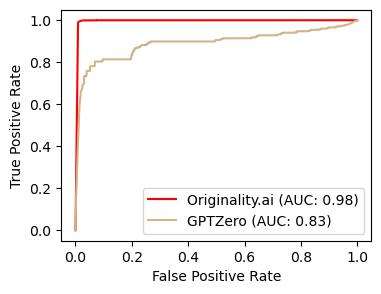
\includegraphics[width=0.4\textwidth]{genai/roc_curve.jpg}
  \caption{This Receiver Operating Characteristic (ROC) curve shows the performance of each detector on our data of known providence (Cycle 2022 submissions and ChatGPT responses to Cycle 2022 prompts). While GPTZero's ROC curve has a moderate area under the curve (AUC), Originality.ai's ROC curve has a very high AUC.}
  \label{fig:roc_auc}
\end{figure}

\subsection{Results}
\subsubsection{Both Detectors Possess the Properties Desired for Low-Stakes Decision Support}
We identified no properties required to support low-stakes decisions, but list several desiderata that we consider more a matter of utility than of necessity. In particular, detectors should have:

\begin{enumerate}
    \item Low cost
    \item High utility
\end{enumerate}

We measure cost as the price per essay evaluated at the highest tier of subscription service available from each detector in Table \ref{tab:detector_cost}. We measure utility according to ROC AUC.

Table \ref{tab:detector_cost} shows that both detectors have low cost, with GPTZero having slightly lower cost.\footnote{As we used both detectors for research purposes, we reached out to the companies involved and were given research access. These cost estimates are based not on our access, but on public information assuming the highest tier of subscription service available from each detector.}

Figure \ref{fig:roc_auc} demonstrates high utility from both detectors, though Originality.ai has a higher ROC AUC than GPTZero. Overall, both detectors satisfy the desiderata specific to low-stakes decisions.

\begin{table}[htbp]
  \centering
  \caption{This table displays estimated per-essay costs of each detector; both detectors are deemed sufficiently cost-effective.}
  \label{tab:detector_cost}
  \begin{tabular}{l r}
      \toprule
      Detector & Cost per Essay \\
      \midrule
      GPTZero & $\$0.023$ \\
      Originality.ai & $\$0.06$\\
      \bottomrule\\
  \end{tabular}
\end{table}

\subsubsection{GPTZero Possesses the Properties Required for High-Stakes Decision Support}\label{sssec:highstakes}
We identified two properties required to support high-stakes decisions. Detectors should have:

\begin{enumerate}
    \item High discrimination
    \item Low bias
\end{enumerate}

We measure discrimination as by whether the detector clearly discriminates positive and negative cases (see Table \ref{tab:detector_cost}). We measure bias as the difference in FPR between demographic groups.

\begin{figure}[htb]
  \centering
  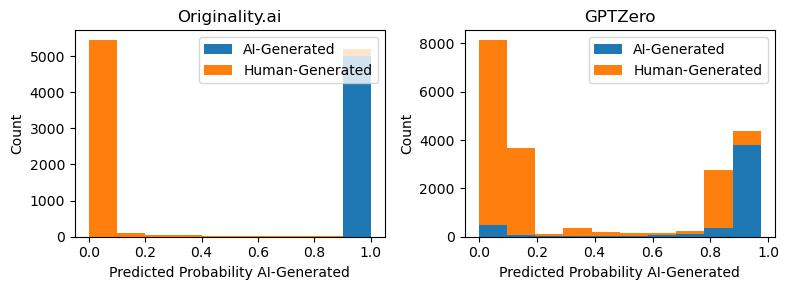
\includegraphics[width=0.8\textwidth]{genai/histogram.jpg}
  \caption{These histograms demonstrate the high bimodality and predictive discrimination of both detectors' outputs.}
  \label{fig:histogram}
\end{figure}

As can be seen in Figure \ref{fig:histogram}, both detectors' outputs are close to either 0 or 1, though Originality.ai has far higher discrimination than GPTZero. This is reflected in the confusion matrices in Figure \ref{fig:confusion}. As can be seen, both output statistics discriminate well between positive and negative cases. However, while GPTZero clearly discriminates between positive and negatives, Figure \ref{fig:confusion} shows that Originality.ai has lower error of both types.

\begin{figure}[htb]
  \centering
  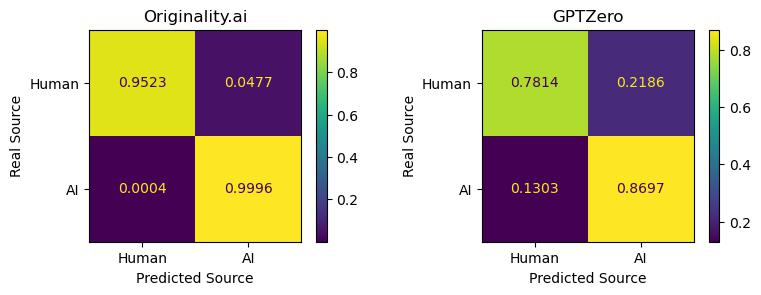
\includegraphics[width=0.8\textwidth]{genai/confusion.jpg}
  \caption{These confusion matrices again demonstrate the high predictive discriminative capabilities of both detectors' outputs.}
  \label{fig:confusion}
\end{figure}

We see bias in both statistics in Table \ref{tab:demo_means_c2}, as the FPRs (average detection statistic on known-human essays) differ by demographic in both cases. Interestingly, though GPTZero has much higher false positive rates in all cases, these rates differ less by demographic than those of Originality.ai (this can be seen in the lower ANOVA statistic). This results in us observing Originality.ai ANOVA statistics $2.75$ and $3.40$ greater than GPTZero ones, respectively. This is, practically, the difference between minor between-group variance and measurable and harmful bias. For this reason, although both detectors have bias, we believe that GPTZero's bias does not render it unsuitable for ex-post decisions across our applicant pool, while Originality.ai's does.\footnote{Note that, in the case of Originality.ai, this appears to be driven by disparate performance across regions (and the ``Other'' gender category). Organisations with more regionally homogeneous applicants may wish to re-analyse Originality.ai's biases across their relevant demographics.} In this case, our partner organisation saw the high risk of false positive from the GPTZero statistic as sub-optimal, but deemed the bias demonstrated by Originality.ai, particularly across different regions, untenable.

\begin{table*}[htbp]
  \centering
  \caption{This table displays FPRs for both detectors split by applicant demographics and compared by ANOVA in the (human-written) Cycle 2022 submissions. Differences in FPR here can be interpreted as bias: both detectors display a bias, but Originality.ai displays a far higher bias than GPTZero.}
  \label{tab:demo_means_c2}
  \begin{tabular}{l r r}
      \toprule
      Demographic Group & GPTZero & Originality.ai \\
      \midrule
      Male                    & $0.23$ & $0.06$ \\
      Female                  & $0.23$ & $0.07$ \\
      Other                   & $0.21$ & $0.16$ \\
      ANOVA Statistic         & $\mathbf{0.11}$ & $\mathbf{2.86}$ \\
      \midrule
      Caribbean               & $0.17$ & $0.00$ \\
      East and Southeast Asia     & $0.24$ & $0.06$ \\
      Core Anglosphere               & $0.21$ & $0.17$ \\
      Eastern Europe / Central Asia    & $0.23$ & $0.17$ \\
      South Asia     & $0.22$ & $0.07$ \\
      Latin America           & $0.21$ & $0.02$ \\
      Middle East / North Africa   & $0.25$ & $0.05$ \\
      Sub-Saharan Africa      & $0.23$ & $0.06$ \\
      Western Europe            & $0.20$ & $0.00$ \\
      Pacific Islands         & $0.04$ & $0.00$ \\
      ANOVA Statistic         & $\mathbf{0.57}$ & $\mathbf{3.97}$ \\
      \midrule
      All Submissions         & $0.23$ & $0.05$ \\
      \bottomrule
  \end{tabular}
\end{table*}

\subsubsection{Both Detectors Possess the Properties Required for Ex-Post Decision Support}
We identified two properties required to support ex-post decisions. Detectors should have:

\begin{enumerate}
    \item Moderate Discrimination
    \item Calibrated Probability\footnote{Calibrated statistics are ones whose distributions are probability-like in expectation.}
\end{enumerate}

We measure discrimination as in Section \ref{sssec:highstakes}. We measure statistic calibration using calibration curves in Figure \ref{fig:calibration}.

We have already determined in Figure \ref{fig:roc_auc} that Originality.ai has particularly high predictive discrimination, while GPTZero has moderate predictive discrimination suitable for ex-post analyses.

\begin{figure}[htb]
  \centering
  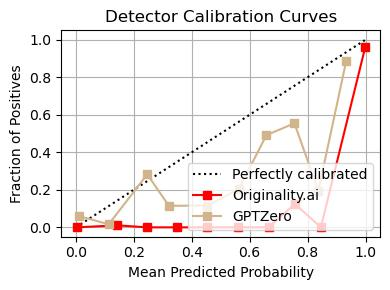
\includegraphics[width=0.4\textwidth]{genai/calibration.jpg}
  \caption{These calibration curves demonstrate the bimodality of both detectors' outputs. As can be seen, both output statistics fall far below the calibration curve; these output statistics are not calibrated on our data.}
  \label{fig:calibration}
\end{figure}

In aggregate analyses, we desire to reason about the probability that a particular essay was generated by AI ($P(AI)$), or even the expected number of AI-generated essays in a given group ($E(P(AI))$). This yields convenient general properties, e.g., $E(P(AI))$ is just the mean $P(AI)$ within a given group. Figure \ref{fig:calibration} provides a calibration curve for both detectors, and demonstrates a comparative lack of calibration in both cases. In both cases, output statistics fall far below the calibration curve, indicating a bias towards extrema. In effect, this entails that we should not treat these output statistics like probabilities. However, so long as we have a large provenance of labelled data (which we do in the form of $15,149$ applicant-submitted and $5,002$ ChatGPT-generated Cycle 2022 essays), we can calibrate an uncalibrated statistic to achieve a more probability-like output. In our case, we calibrate our statistics on our data by applying a monotonic transformation to ensure that, within any subset of our body of essays, the mean predicted probability aligns with the fraction of positive cases.

Thus, we conclude that, post-calibration, both detectors possess the properties of probabilities that we would require for use in ex-post analyses. We caution other organisations against using these detectors for these purposes without first calibrating their output statistics on data of known provenance.

\subsubsection{Neither Detector Possesses the Properties Required for In-Process Decision Support}
We identified four properties required to support in-process decisions. Detectors should have:

\begin{enumerate}
    \item Minimal Bias
    \item Interpretable Outputs
    \item Acceptable Performance at Low FPR
    \item Bimodal Statistic
\end{enumerate}

We measure bias as in Section \ref{sssec:highstakes}. We reason about model interpretability. We measure acceptable performance at low FPR based on TPR rates at an FPR of $\%1$. We measure bimodality using the histogram in Figure \ref{fig:histogram} and the calibration curve in Figure \ref{fig:calibration}.

Recall that, in Table \ref{tab:demo_means_c2}, we observe bias in both outputs, and conclude that, while GPTZero is sufficiently balanced across demographic groups, Originality.ai's outputs display too much regional bias for our purposes. 

We also note that GPTZero provides interpretability in the form of local-level scores that might direct a human overseer's attention to particularly problematic phrases or sentences. Originality.ai, in contrast, only provides a single overall statistic. 

Figure \ref{fig:histogram} demonstrates the bi-modality of both detectors. Though it is clear that Originality.ai's output is more bimodal, we consider both detectors sufficiently bimodal for our purposes.

\begin{table*}[htbp]
  \centering
  \caption{This table displays TPRs at $\%1$ FPR.}
  \label{tab:tprs}
  \begin{tabular}{l r r}
      \toprule
      Detector & TPR \\
      \midrule
      GPTZero & $\%36.0$ \\
      Originality.ai & $\%98.9$ \\
      \bottomrule
  \end{tabular}
\end{table*}

Finally, to analyse performance at low FPR, our organisation set the acceptable FPR at $\%1$. We see TPR of $\%36.0$ for GPTZero and $\%98.9$ for Originality.ai in Table \ref{tab:tprs}. While GPTZero's output statistics are interpretable and display limited bias, it fails at low FPR rates.

\begin{figure}[htbp]
  \centering
  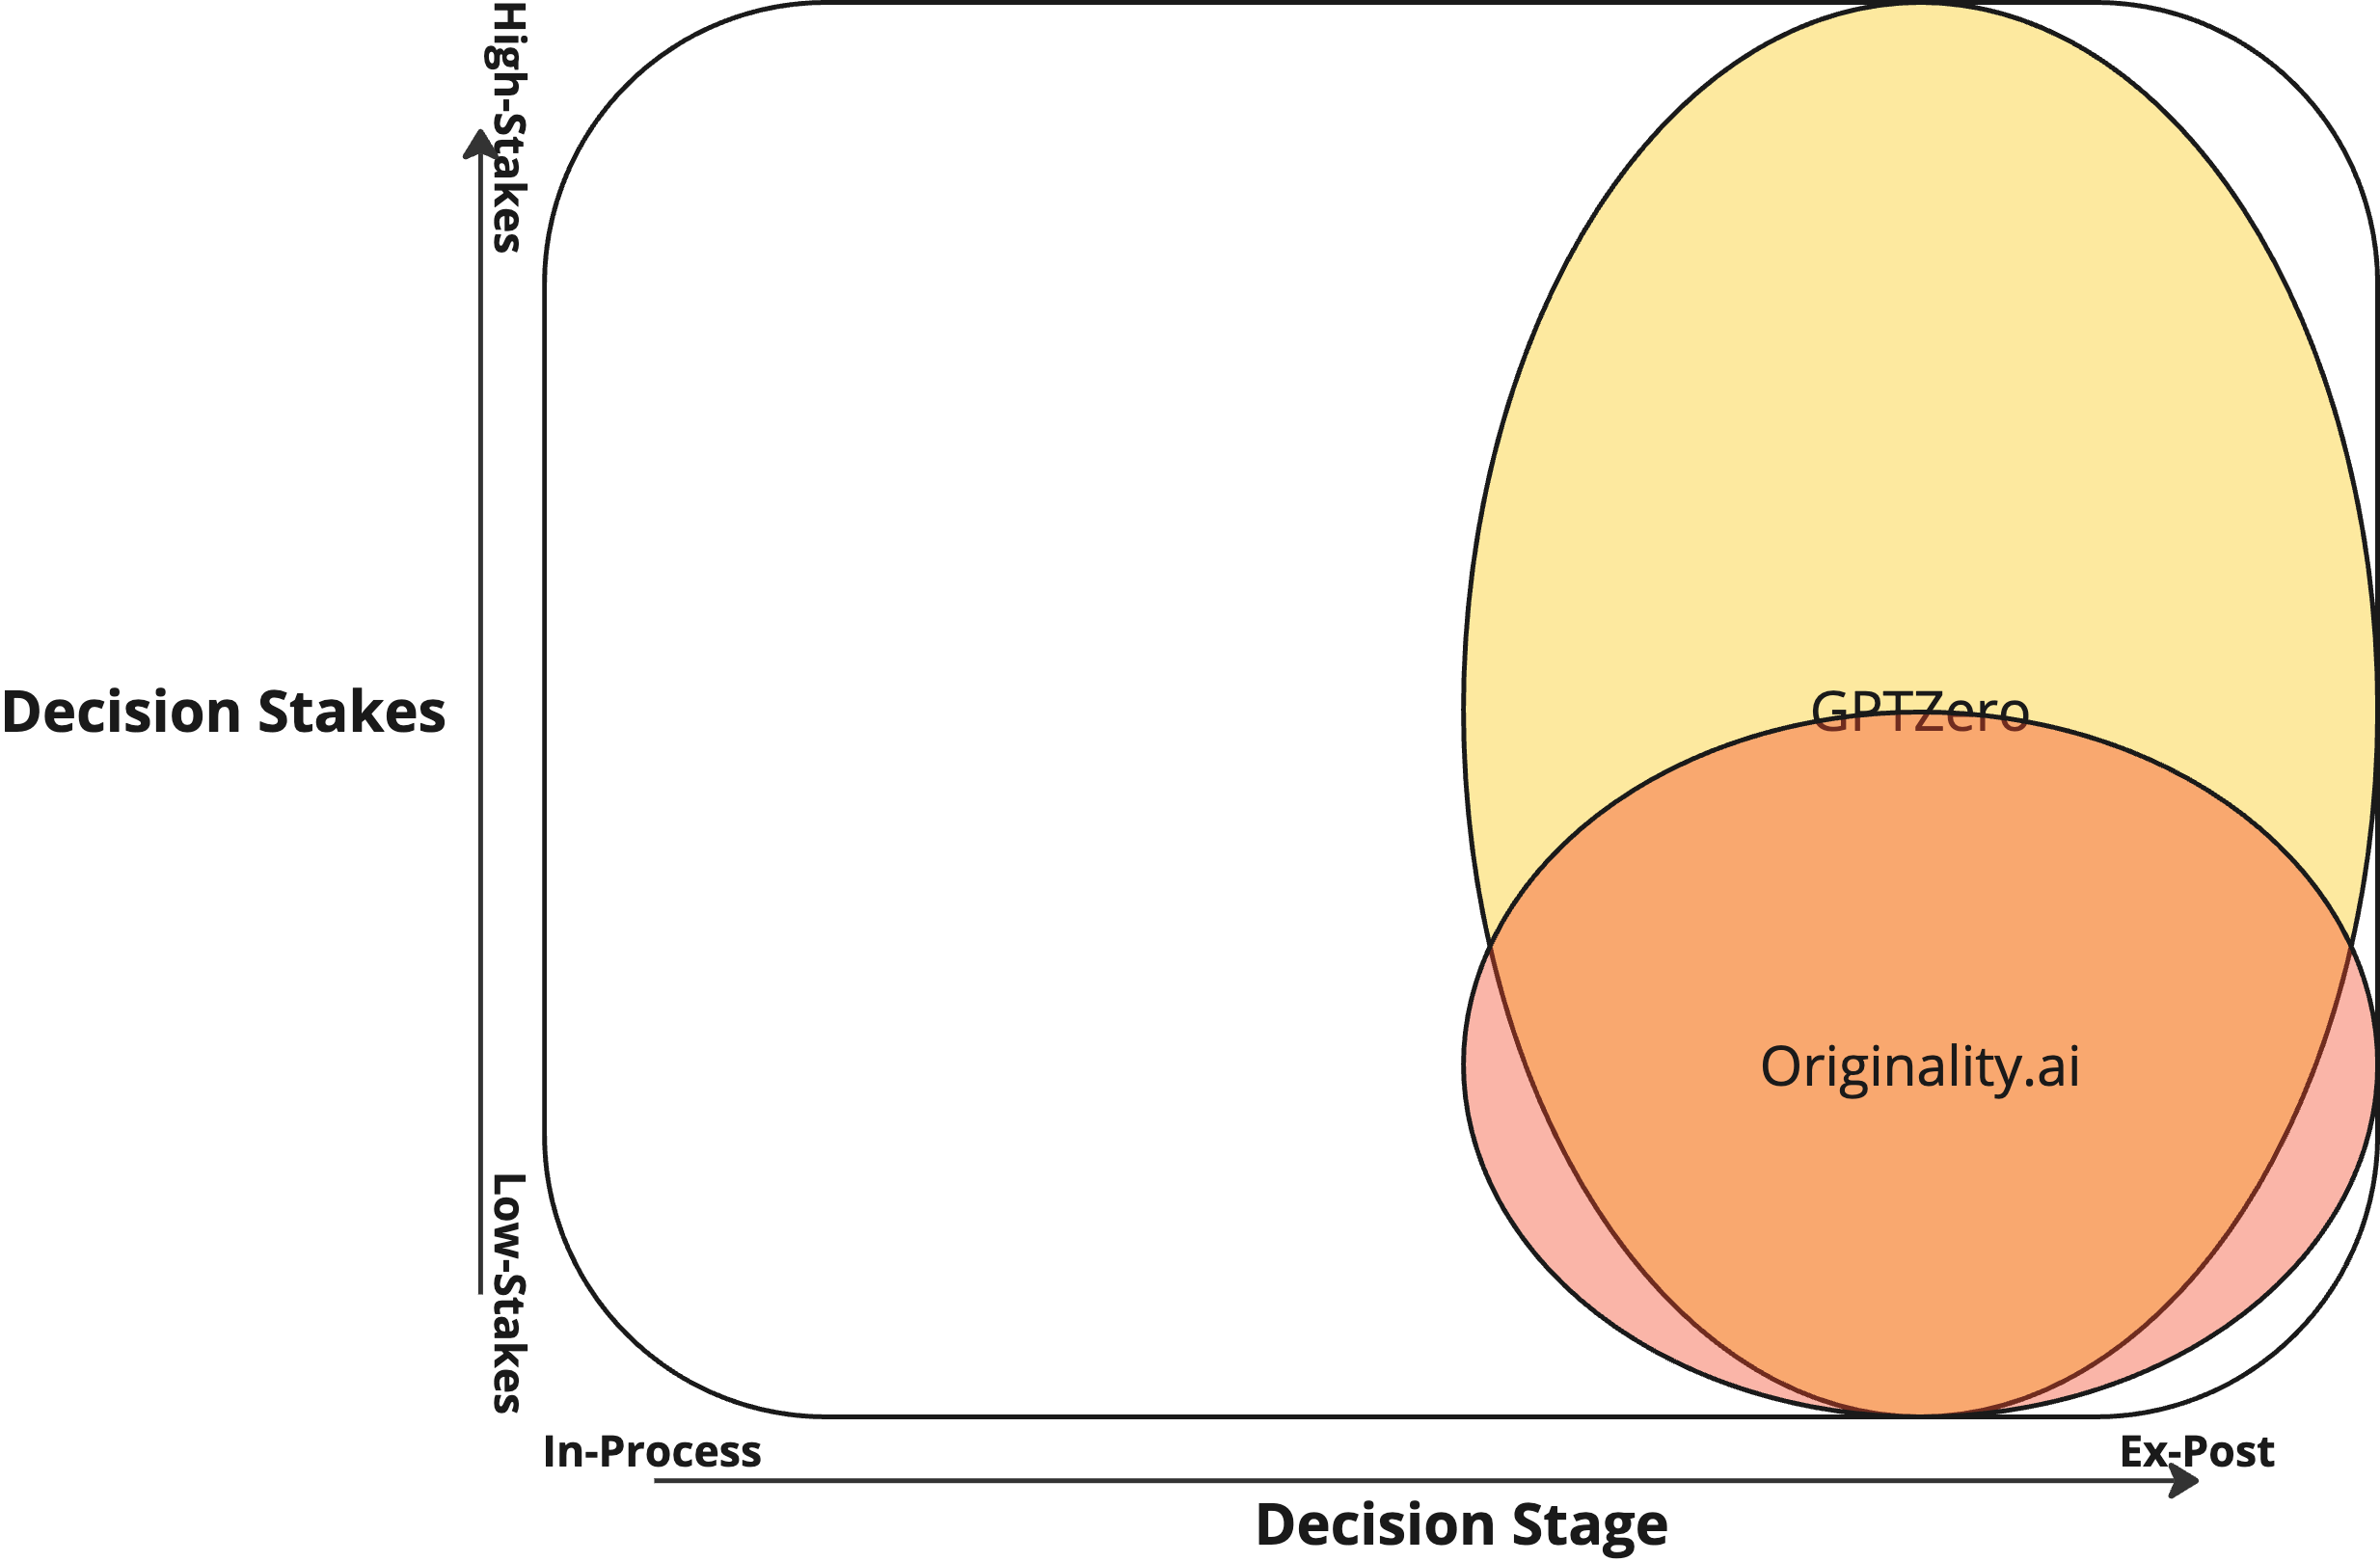
\includegraphics[width=0.8\textwidth]{genai/satisfaction_matrix.png}
  \caption{This figure demonstrates the results of our application of the Decision Matrix, marking the use cases we consider suited for each detector.}
  \label{fig:satisfaction_matrix}
\end{figure}

\section{Analysis of \emph{Pipeline} and \emph{Partners}}\label{ssec:decisions}

\subsection{Low-Stakes Ex-Post: Analysing Overall GenAI Usage in the 2023 Application Cycle (\emph{Pipeline})}
We focus our subsequent analysis primarily on the potential use of genAI by applicants in Cycle 2023. Seeking to avoid the disproportionate effects induced by GPTZero's heterogeneous biases (see Table \ref{tab:demo_means_c2}), we focus primarily on within-group changes. We note here that the mean probability of an essay being AI-generated within a corpus is exactly the expected proportion of AI-generated content within that corpus. Thus, we test for changes in mean $P(AI)$. As we have previously confirmed GPTZero is suitable for these analyses, we use our calibrated GPTZero score going forward. Table \ref{tab:demo_means_c23} presents mean $P(AI)$ for 2023 (column 3) and 2022 (column 5), as well as test statistics of whether there is a difference in means (columns 6 and 7). 

\begin{table*}[htbp]
  \centering
  \caption{These t-tests comparing $\widehat{E(P(AI))}$ across the 2022 and 2023 application cycles for each demographic reveal several changes by demographic, but only a small overall increase in AI-generated content.}
  \label{tab:demo_means_c23}
  \begin{tabular}{l r r r r}
      \toprule
      & Cycle 2022 & Cycle 2023 & \multicolumn{2}{c}{Inter-Cycle $\Delta$} \\
      Demographic Group & $\widehat{E(P(AI))}$ & $\widehat{E(P(AI))}$ & Test Statistic & p Value \\
      \midrule
      Male    & $0.09$ & $0.11$ & $\mathbf{8.63}$ & $\mathbf{<0.01}$ \\
      Female  & $0.11$ & $0.11$ & $-0.40$ & $0.69$ \\
      Other   & $0.14$ & $0.12$ & $-1.10$ & $0.27$ \\
      \midrule
      Caribbean               & $0.17$ & $0.15$ & $-0.47$ & $0.64$ \\
      East and Southeast Asia     & $0.13$ & $0.13$ & $0.74$ & $0.46$ \\
      Core Anglosphere               & $0.21$ & $0.14$ & $\mathbf{-5.86}$ & $\mathbf{<0.01}$ \\
      Eastern Europe / Central Asia     & $0.13$ & $0.15$ & $0.59$ & $0.56$ \\
      South Asia     & $0.08$ & $0.09$ & $\mathbf{2.65}$ & $\mathbf{0.01}$ \\
      Latin America           & $0.13$ & $0.09$ & $-1.44$ & $0.15$ \\
      Middle East / North Africa   & $0.11$ & $0.12$ & $1.67$ & $0.09$ \\
      Sub-Saharan Africa      & $0.09$ & $0.09$ & $\mathbf{2.15}$ & $\mathbf{0.03}$ \\
      Western Europe            & $0.20$ & $0.12$ & $\mathbf{-2.75}$ & $\mathbf{0.01}$ \\
      Pacific Islands         & $0.04$ & N/A      &  &  \\
      \midrule
      All Submissions         &$0.10$ & $0.11$ &  &  \\
      \bottomrule
  \end{tabular}
\end{table*}

We find statistically significant increases in the $P(AI)$ for only two overlapping subgroups: male applicants and applicants from the Indian subcontinent. In both cases the magnitude of the increase is small, suggesting that at least in Cycle 2023, the use of genAI was limited. However, other findings preclude interpreting this change as a direct measure of increased genAI use. In two regions, the Core Anglosphere and Western Europe, we found a statistically significant decrease in the calibrated estimated probability that essays were completely AI generated. Since we can assume very few if any applicants in Cycle 2022 had access to genAI, this cannot be interpreted as a decrease in AI use. It may be that both regions' high average scores in 2022 were a fluke of the cohort, and that these regions reverted to the mean in 2023. Alternatively, it is possible that, in these regions, Cycle 2023 applicants used AI detection tools to ensure that their content would not be flagged by our detector (although this would require such detector usage to offset any actual genAI use) \cite{gptzero_gptzero_2023}. In either case, this analysis surfaces interesting discrepancies demanding further interrogation in future cycles, but does not demand the program alter their application material or process.

\begin{table}[htb]
    \centering
    \caption{This Tukey's Honestly Significant Difference (HSD) test looks for differences in the proportion of predicted AI-generated essays across different program channel partners in the 2023 application cycle, but finds no evidence of any channel partners' applications being more likely to be AI-generated than the average.}
    \label{tab:c3_partner_anova}
    \begin{tabular}{ c c c c c }
        \toprule
        \multicolumn{3}{c}{} & \multicolumn{2}{c}{HSD Results} \\
        \cmidrule(lr){4-5}
        Channel Partner & Essays & Share `AI-Generated' & Test Statistc & p Value \\
        \midrule
        Partner A & $540$ & $0.041$ & $0.064$ & $0.80$ \\
        Partner B & $390$ & $0.044$ & $0.004$ & $0.95$ \\
        Partner C & $325$ & $0.049$ & $0.320$ & $0.57$ \\
        Partner D & $315$ & $0.029$ & $1.599$ & $0.21$ \\
        Partner E & $235$ & $0.064$ & $2.526$ & $0.11$ \\
        Partner F & $205$ & $0.039$ & $0.076$ & $0.78$ \\
        Partner G & $170$ & $0.047$ & $0.071$ & $0.79$ \\
        Partner H & $150$ & $0.027$ & $0.970$ & $0.33$ \\
        Partner I & $150$ & $0.007$ & $\mathbf{4.829}$ & $\mathbf{0.03}$ \\
        Partner J & $135$ & $0.022$ & $1.415$ & $0.23$ \\% can surpress to save space
        \midrule
        All Submissions & $24,815$ & $0.040$ & \\
        \bottomrule
    \end{tabular}
\end{table}

\subsection{High-Stakes Ex-Post: Analysing GenAI Usage in the Program's 2023 Channel (\emph{Partners})}
As a final analysis, we evaluate whether GPTZero detects any suspicious patterns in the essays associated with the program's channel partners, who refer and support applicants to the program. The organisation partners with `channel partner' organisations that encourage applications and these are attributed to channel partners based on the custom links applicants use to reach the program's website, as well as questions in the application about how applicants learned of the program. Evidence that any of these channel partners used genAI to create large volumes of applications would warrant further investigation before continuing affected partnerships. 

For this analysis, we use a cutoff of $0.5$ on our calibrated predictor, meaning that essays flagged as `AI-Generated' are more likely than not to be so. This threshold has a TPR of $76\%$ and a FPR of $4\%$. We limited analysis to the partners with the most essays and have hidden individual partners' identities.

As Table \ref{tab:c3_partner_anova} shows, only one of the channel partners studied was associated with essays identified as AI-generated at a rate meaningfully different from the overall pool. However, the partner in question, Partner I, was actually associated with fewer essays than average identified as AI-generated. This could be driven either by the chance of finding at least one statistically significant result when testing multiple hypotheses or by the partner, based in sub-Saharan Africa, working primarily with demographics identified in Cycle 2022 analyses as naturally having below-average calibrated scores. In either case, we find no evidence of widespread genAI use among the program's channel partners, supporting the organisation's channel partnership approach and choice of partners.

\section{Discussion}\label{sec:genaidisc}
\subsection{Implications for the Program}
The program we work with has a number of use cases for genAI detection, and we have found that GPTZero is suitable for the ex-post use cases, both high- and low-stakes. However, the program's use of genAI detection for in-process decisions is not yet feasible, as, although Originality.ai has a very high accuracy, it suffers from a lack of interpretablity and its FPRs exhibit large heterogeneous biases across demographics, especially region. We recommend that the program continue to use GPTZero for ex-post decisions, but that it seek out a new detector or design their own if they wish to make data-driven, in-process decisions surrounding genAI usage. A summary of our recommendations can be found in Figure \ref{fig:satisfaction_matrix}.

\subsection{Implications for Other Programs}
By identifying decision points, placing them on the Decision Matrix, aligning these desired and required properties, then testing genAI detection tools for the relevant properties, programs can determine the suitability of detectors in supporting and informing decision points. If a program's decision points and desired properties align closely with our partner program's, they may find that they consider the same use cases for GPTZero and Originality.ai, and have no need for our framework. But if the genAI detection landscape changes in response to new developments \cite{ashish_vaswani_attention_2017,jacob_devlin_bert_2018,openai_gpt-4_2023,liang_gpt_2023,mitchell_detectgpt_2023,liu_deid-gpt_2023,kalpesh_krishna_paraphrasing_2023}, or if programs' priorities do not align with those of our partner organisation, programs should use the Decision Matrix framework to replicate the analysis done here.

\subsection{Implications for the Field}
Our results suggest that, while genAI detection tools address some issues faced by scholarship selection practitioners, deeper involvement with these institutions is key in designing technology to meet the specific needs of these practitioners. Currently, a narrow focus on academic integrity, plagiarism, and decisions to censure essay-writers limits broader discussions about how genAI should be integrated into academic workflows. While practitioners shift towards embracing genAI as a tool rather than a threat, the field of HCI is lagging behind. 

Our AR process raises the question: should it matter whether genAI was used at all? Rather than aiming to detect AI-generated plagiarism, selection practitioners are perennially concerned with determining whether an applicant's submission indicates their aptitude for the program; the need for detector-based decision support, in all cases, is to support decisions impacting that ultimate determination. GenAI tools pose problems to practitioners' abilities to make that determination with contemporary essay-based assessment, but outright bans and disqualification \cite{h_holden_thorp_chatgpt_2023} unenforceable with current technology offer no solutions. A shift in assessment methodology, then, is a practical and desirable alternative.

HCI and genAI detection can enable this shift through respectful design \cite{VanKleek_Seymour_Binns_Shadbolt_2018} by working with selection practitioners to understand their needs and support them (e.g., by improving assessment design or by building digital feedback mechanisms). Institutions, meanwhile, may wish to design essay prompts that encourage or even require applicants to use genAI in a meaningful way. In such cases, the role of detectors would shift from merely identifying AI-generated content to evaluating how well applicants have leveraged these technologies.

\subsection{Ethical Implications}
The Decision Matrix framework developed throughout the paper reveals a variety of desiderata for the usage of genAI detectors in application essay settings. As can be seen in Figure \ref{fig:desiderata_matrix}, the decision to disqualify a candidate demands much of detectors. Indeed, even when detectors possess all of the desired properties, taking automated adverse action against applicants is ethically fraught \cite{Lashkari_Cheng_2023}. However, when opting to make no decisions about applicants using this technology, these demands fall away.

In practice, our research sits between these extrema. The process of holistic review sees organisations incorporate a mass of disparate information into an opaque decision-making process. \textcite{hirschman_dequantifying_2016} note this lack of transparency as a benefit of holistic review insofar as it shields institutions from regulators. But while this may offer holistic review some legal insulation, no such moral insulation exists. In-process algorithmic decision support, even for low-stakes decisions such as \emph{Diligence}, still bears a high moral burden \cite{Lashkari_Cheng_2023}.

\section{Limitations and Future Work}
One participant highlighted: ``There are two problems here: Did this applicant use [generative AI]? And if so, is this essay based in fact?''. This points to a key limitation of our evaluation of detectors: while we could determine whether text was AI-generated, we had no basis for evaluating the truthfulness of AI-generated text. As genAI is known for its hallucination \cite{alkaissi_artificial_2023}, frequently yielding convincing falsehoods, this represents a significant limitation. While this distinction is ultimately irrelevant to those who consider an genAI usage plagiarism \cite{h_holden_thorp_chatgpt_2023}, decisions such as \emph{Diligence} would be well-informed by an understanding of how genAI was used. Future work should investigate detecting the nature of genAI usage (writing, editing, etc.) and then determining the truthfulness of genAI-written text.

As we select only two detectors, our results as applied to these detectors may not be applicable to others. Furthermore, as the field of genAI detection moves so rapidly, our results from Cycles 2022 and 2023 may not even apply to Cycle 2024. For this reason, we develop the Decision Matrix framework to support ongoing evaluations of detectors in response to new developments such as paraphrasing tools and hybrid human-genAI writing processes \cite{kalpesh_krishna_paraphrasing_2023}. Future work should use this framework in re-evaluating detectors in response to these new developments.

We deliberately do not engage applicants in our process. \textcite{venn-wycherley_realities_2024} argue that, when conducting human-centred research in a classroom setting, it is important to gather perspectives of both educators and students. Here, we conduct AR centred on scholarship selection practitioners, but we omit the perspectives of their young decision subjects. Unlike in the classroom context, the evaluation context sees an adversarial relationship between the educational institution and its target population – while the scholarship seeks to select only the most well-fit candidates, each candidate seeks to be selected, and therefore to make themselves seem most fit. Thus, in making the selector ``Co-investigators of, co-participants in, and co-subjects of'' our research \cite{Hayes_2011}, we necessarily exclude the perspectives of their decision subjects. Future work should seek to engage these young decision subjects in this context, and may explore concepts like the essayist's sense of authorship, the line between writing and editing, essayist thoughts on plagiarism, and applicant perceptions of program decisions driven by AI.

\section{Conclusion}
In summary, this research examines the various decisions that may arise when scholarship selection organisations consider the problems posed by genAI in practice, emphasising the need for tools designed to support decisions besides simply disqualifying applicants. Our findings reveal that, although state-of-the-art detectors may be unsuitable as automated disqualification tools, they can be used as-is to support ``integrating technology, education, policy reform, and assessment restructuring'' \cite{MikePerkins_JasperRoe_2023} and support ex-post decisions organisations may wish to make. By engaging in action research, we catalogued real decisions scholarship selection organisations seek to make in response the problems posed by genAI usage. We then worked with them to develop the Decision Matrix, which serves as a tool for practitioners to evaluate genAI detectors on their data. As we move forward, we call for a broader view of the purpose of genAI detection, and for a restructuring of what it is to learn and assess in an era so heavily influenced by easy access to genAI tools.
% \begin{savequote}[8cm]
% Alles Gescheite ist schon gedacht worden.\\
% Man muss nur versuchen, es noch einmal zu denken.

% All intelligent thoughts have already been thought;\\
% what is necessary is only to try to think them again.
%   \qauthor{--- Johann Wolfgang von Goethe \cite{von_goethe_wilhelm_1829}}
% \end{savequote}

\chapter{\label{ch:diversity}``Diversity is Having the Diversity'': Unpacking and Designing for Diversity in Applicant Selection}

\minitoc

\begin{figure}
    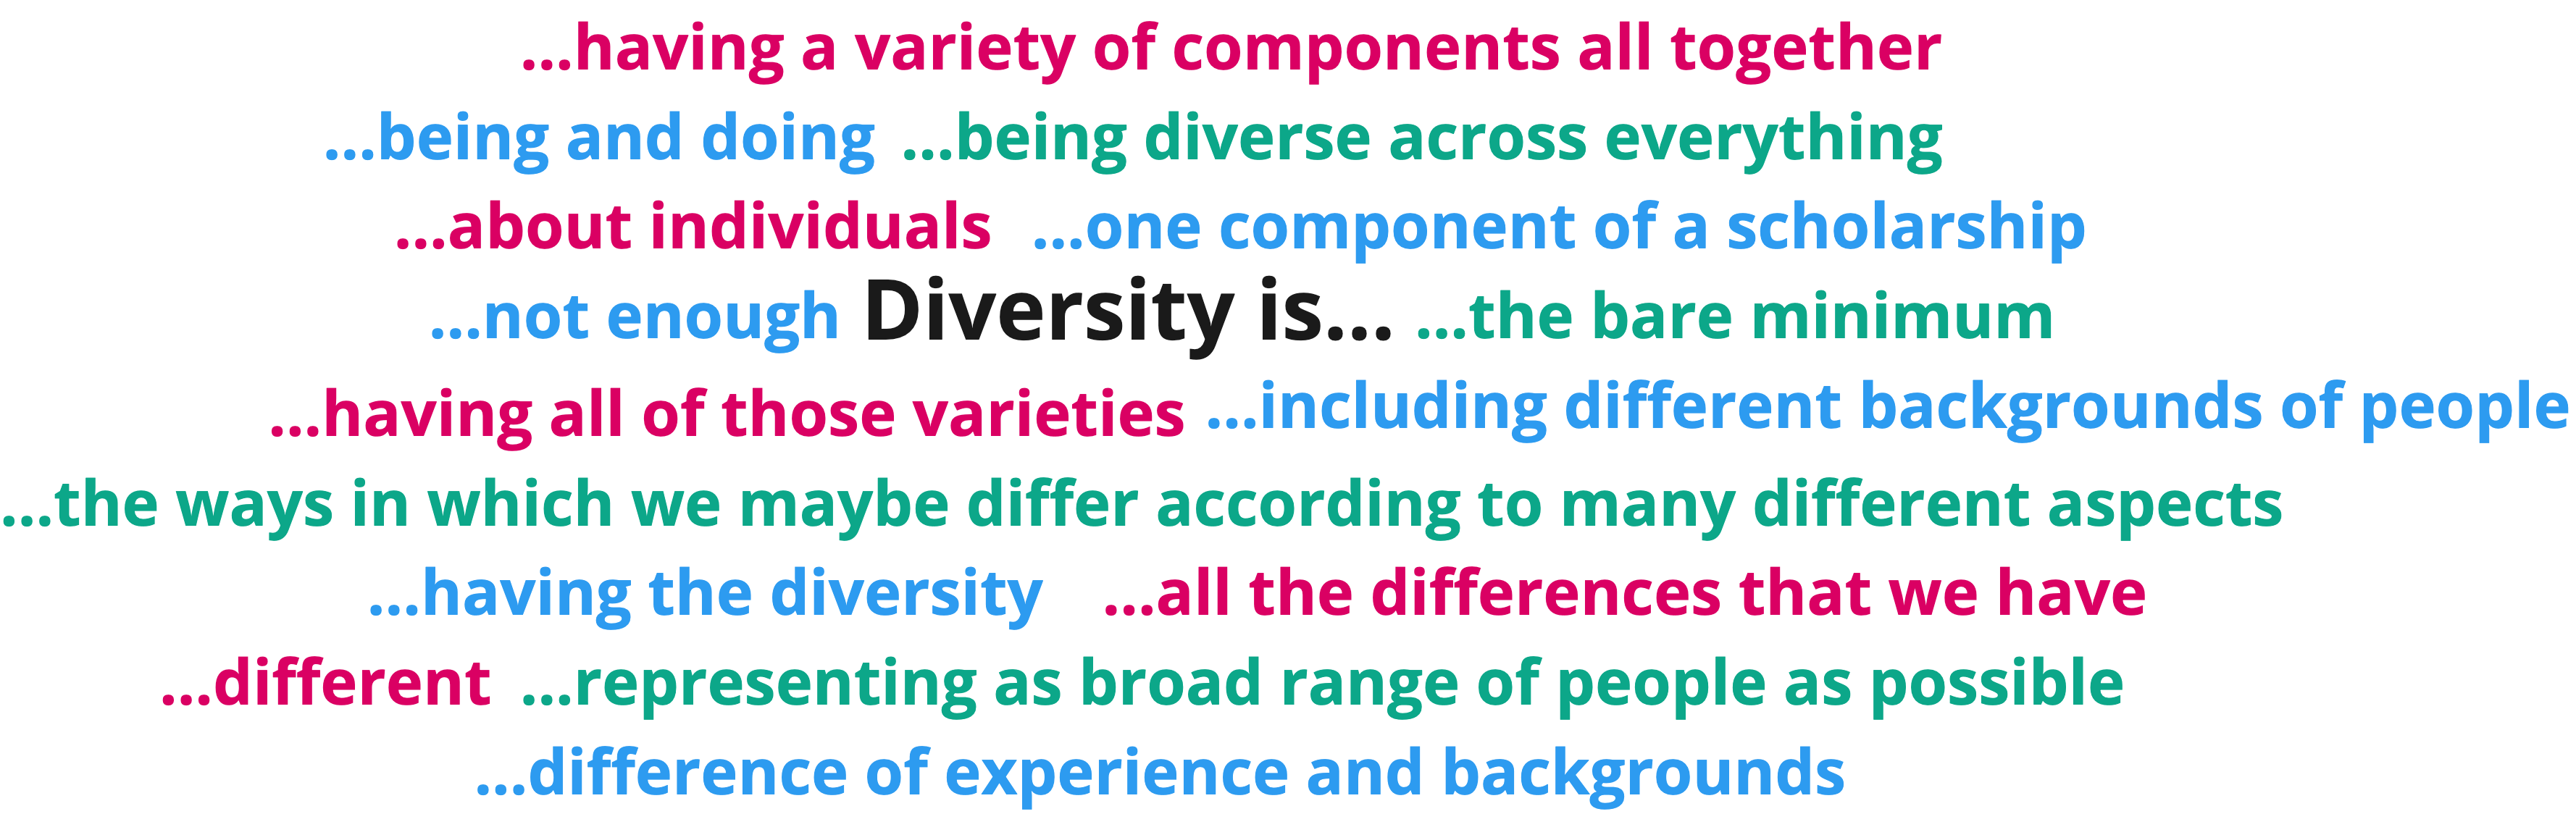
\includegraphics[width=\textwidth]{diversity/diversity_is.png}
    \caption{This figure shows participant codes defining what ``diversity is''. In this chapter, we seek to answer: what do they mean and how do we design for that?}
    \label{fig:diversity_is_teaser}
\end{figure}
  
\section{Introduction}\label{sec:divintro}
Processes for selecting people for jobs, universities, prizes, and other opportunities have often failed to reflect the diversity of their actual and potential candidate pool. Recognising this, various sectors have in recent years shifted towards recognising and promoting diversity through the establishment of a variety of related norms: DEI (Diversity, Equity, and Inclusion), EDI (Equality, Diversity and Inclusion), JEDI (Justice, Equality, Diversity, and Inclusion), DEIB (Diversity, Equity, Inclusion, and Belonging), etc. \cite{pinkett2023data,hsieh2019allocation,minkin2023diversity}. These norms are frequently operationalised through changes to application, evaluation, and decision-making procedures designed to result in greater representation of different demographic groups in final selection decisions \cite{pinkett2023data}. Such efforts are in part a response to widespread societal concerns about racial, gender, and other injustices, but have also frequently been justified in economic terms by evidence suggesting that diverse teams perform better than homogeneous ones on a variety of tasks \cite{deming2017growing,page_diversity_2017,noray2023systemic}. Meanwhile, the concept of diversity itself has become swept up in `culture war' discourse, criticised by right wing commentators as part of a sinister `woke' agenda, and by progressives as mere window dressing which fails to meaningfully address deeper societal injustices. 

However, for practitioners involved in selection processes on the ground, the question of how to meaningfully measure and promote diversity in their decisions is a real and challenging one. The proliferation of software to help with hiring and talent selection – in the form of application management platforms, decision-support tools, and more recently, widespread use of AI – provides additional complications, as well as potential opportunities \cite{Lashkari_Cheng_2023}. For instance, AI-driven tools may discriminate against candidates who don't resemble their training data \cite{chen2018investigating,li2020hiring,lambrecht2019algorithmic}; but they could potentially assist in mitigating human biases in recruitment and selection processes, resulting in greater diversity \cite{yarger2020algorithmic,avery2024does,will2023people, suhr2021does}. This context thus challenges Human-Computer Interaction (HCI) and Human-Centred Artificial Intelligence (HCAI) research to improve diversity in selection processes without amplifying or codifying pre-existing inequities.

But to improve diversity in selection processes, we must first understand it. We undertake two studies to do just that. In Study 1, we conducted 15 one-to-one interviews with scholarship and talent investment selection practitioners (selectors). All participants were involved in scholarship selection for an international cohort of students in a global academic programme. We aimed to understand how these practitioners define and operationalise diversity and how technology can aid this process. Each interview lasted 45 minutes. We analysed this data following \textcite{braun_using_2006}'s inductive thematic analysis methodology. Our analysis highlighted the ad-hoc nature of current diversity considerations and the need for more structured, data-supported approaches, and surfaced three distinct definitions of diversity: one involves placing people with `different perspectives' in the same room; another, ensuring `representativeness' of some target population; a third, `contextualising applications', e.g., with information such as the applicants' relative privilege or required level of support. We conclude that technological interventions designed to promote diversity in selection processes should first identify specific definition(s) of diversity they aim to promote; we construct the \emph{Diversity Triangle} (Figure \ref{fig:div_triangle}) as a guide.

For Study 2, we developed six design prototypes for diversity-supporting tools based on the Diversity Triangle from Study 1 \cite{Buchenau_Suri_2000}. The prototypes included tools for visualising cohort representativeness, measuring entropy (average number of in-group differences), and assessing individual applicant (dis)advantage scores. They were presented to participants via participatory design workshops \cite{Zimmerman_Forlizzi_2017}. Participants provided feedback on the utility and integration of these tools into their selection processes. The workshops revealed that participants use specific, idiosyncratic lenses to navigate their diversity considerations, and that while quantitative tools are essential for making informed decisions, qualitative assessments remain crucial.

This research contributes to the understanding of how diversity can be supported through data-driven tools in selection processes. Specifically, our contributions are:

\begin{enumerate}
    \item Three definitions of diversity that impact selectors' decisions uncovered through inductive thematic analysis.
    \item The Diversity Triangle, categorising diversity-related themes according to our definitions of diversity.
    \item Design recommendations grounded in participatory design for system implementers supporting the diversity needs of a given organisation.
\end{enumerate}

\noindent More broadly, this work demonstrates that providing structured, data-supported approaches to diversity, organisations can better navigate the complexities of DEI (EDI, JEDI, DEIB, etc.). While differing in some respects, we believe these implications will generalise from scholarship selection to various other talent identification contexts, including recruitment for jobs and admission for universities. By helping these organisations achieve their desired outcomes in selection processes, we ultimately contribute to and help build a more diverse society.

\section{Background}\label{sec:back}
\subsection{Diversity as a societal and organisational value}\label{ssec:value}
Despite its global reach, contemporary discourse on diversity derives (in large part) from the political context of the United States in the latter half of the 20th century \cite{nkomo2019diversity}. Civil rights activists identified gender, race, disability, and other forms of group identity as loci of discrimination and oppression, and constructed political actions around these identities \cite{morris1984origins}. This yielded civil rights laws, including equal treatment laws to protect applicants from discrimination (e.g., in employment). \textcite{nkomo2019diversity} argue that this initial, U.S.-centric perspective on anti-discrimination in the workplace, which focused on under-representation of women and racial minorities, has evolved into a more global concept of diversity encompassing a variety of identities. With an increase in social pressure for representation, organisations increasingly prioritise diversity in their selection procedures \cite{hsieh2019allocation,minkin2023diversity}.

But social and political pressures do not uniformly push for diversity. Critics on all sides challenge the value of diversity, both to organisations and society. \textcite{Ahmed_2012} argues that organisational prioritisation of diversity often limits their appetite to prioritise more meaningful changes. The attention paid to diversity may encourage organisations to merely document social injustice, rather than do something to change it \cite{Ahmed_2012,Rossi2020-ROSWNA-2}. Worse, \textcite{Warikoo_2019} argues that diversity among elite institutions reinforces social injustices. On the other side, critics such as \textcite{Goodhart} position diversity as opposed to the obligations of a good society, while others position this as less a rejection of `diversity' than a rejection of `bad diversity' \cite{lentin_Multiculturalism_2011}.

However, political struggles and social pressure for greater equality are not the only motivation for pursuing diversity. More recent discourse and research has also emphasised the instrumental benefits that greater diversity can bring to workplaces and institutions. While it is sometimes assumed that diversity could reduce the quality of a workforce or cohort by favouring more diverse but `worse' candidates, research on selection processes suggests many organisations can both improve the diversity of their organisations and select `better' candidates (as measured by their own metrics) \cite{autor2008does,noray2023systemic}. Generally, research on the performance of diverse teams yields mixed results \cite{daubner2017dovetailing,page_diversity_2017,noray2023systemic,muller_learning_2019}.

Other arguments in favour of diversity emphasise its benefits in the context of knowledge production. For instance, a long strand of work in philosophy of science and social epistemology has made the case for diversity as key to success in epistemic communities \cite{mill1998liberty,merton1942note,wylie2006introduction}. While diversity in this context often refers to cognitive diversity rather than demographic diversity, the latter may often precede the former, as: ``membership in different social groups (e.g., gender or race) often comes with different task-relevant information, perspectives, or experiences'' \cite{peters2021hidden}. For instance, in biomedical science, inclusion of scientists from more diverse backgrounds could lead to ``novel findings and treatment of diverse populations'' \cite{swartz2019science}.

More generally, ``the more robust a community’s mechanisms for bringing diverse perspectives to bear on epistemic questions of public import, the more effective it is in generating and ensuring responsiveness to all the information and insights held by its members'' \cite{wylie2006introduction}. A related argument is that marginalised groups may occupy epistemically advantageous standpoints when it comes to understanding unjust power structures \cite{harding2004feminist,dror2023there,steel_multiple_2018}, as they may have more informative experiences of oppression \cite{mills2015blackness}, and incentives to learn about it \cite{jaggar1983feminist}.

\subsection{Defining and Measuring Diversity}
With the wealth of disparate motivations for diversity, it is unsurprising that its definition is often unclear. \textcite{page_diversity_2010} offers a helpful generic definition of diversity: ``The heterogeneity of elements in a set in relation to a class that takes different values, such as species in an eco-environment, or ethnicity in a population''. While suitably broad, this definition lacks the specificity required to build supporting technologies \cite{hupont2021diverse,page_diversity_2010}. 

However, different means of measuring diversity appear to offer vastly differing accounts of specific definitions. For instance, the natural way to measure diversity, on \textcite{page_diversity_2010}'s definition, is to report percentages of those different elements, e.g., demographics in a population. But in scientific fields like biology and ecology, diversity is often measured with different methods and occasionally conflicting results \cite{xu2020diversity}. Some use measures from information theory (including entropy measured through the Shannon index \cite{shannon1948mathematical}); others adapt the Herfindahl-Hirschman Index \cite{rhoades1993herfindahl}, commonly used to measure economic market concentration \cite{budescu2012measure,acuna2021ai,shannon1948mathematical,rhoades1993herfindahl}.

Another complication arises when we consider the relationship between diversity and similar notions from AI ethics like fairness: are these really distinct concepts, or do they collapse into each other?
\textcite{zhao2023fairness} argue that ``fairness works can be re-interpreted through the lens of diversity, and strategies enhancing diversity have proven efficacious in improving fairness''. If we assume this re-interpretation, algorithmic fairness literature implies another approach to measuring diversity in constraining model outputs to equalise the performance (i.e., positive predictions) between different demographic groups \cite{barocas2023fairness}. And, though many of these measurements are defined for non-human notions of `diversity' (e.g., diversity of items in a recommender system or diversity of flora in an ecosystem), HCI and related research communities often apply these measurements to human notions when measuring the diversity of participants for research, records for AI training data or backgrounds of authors of published papers \cite{linxen2021weird,himmelsbach2019we,zhao2024position,rojas2022dollar,acuna2021ai}. 

More practical criticisms of measurement and implementation of notions of diversity often point to this confusion. \textcite{steel_multiple_2018} argue that disparate definitions of diversity: ``Can generate unclarity about the meaning of diversity, lead to problematic inferences from empirical research, and obscure complex ethical-epistemic questions about how to define diversity in specific cases''. Similarly, \textcite{abdu2023empirical} caution that the specifics of measurement are, at least in the context of race: ``a value-laden process with significant social and political consequences''. And, if done poorly, this measurement process may exclude already marginalised groups (e.g., gender-fluid or mixed-race individuals) \cite{scheuerman2019computers}. While poor categorisation is harmful in any context, larger institutions must be doubly cautious, as, in using constructs to measure diversity, they may inadvertently reify them as natural rather than social \cite{scheuerman2021auto}. 

\subsection{AI and Decision Support Systems for Hiring and Talent Selection}
While there is good reason to express scepticism towards predictive technology in recruitment, \textcite{Vereschak_Alizadeh_Bailly_Caramiaux_2024} demonstrate that, so long as AI systems prove trustworthy and well-designed, decision-makers will engage with and rely on these systems. Apprehension with these systems range from concerns about bias to a disquiet about a distance between applicant and organisation \cite{Lashkari_Cheng_2023}. While concerns about biased AI systems can also be directed at human reviewers, the distance between applicant and organisation created by the introduction of automated decision support tools must be more carefully managed \cite{Leung_Zhang_Jibuti_Zhao_Klein_Pierce_Robert_Zhu_2020,Lashkari_Cheng_2023}. Ultimately, flaws in present pipelines point to the need for better systems, and, despite a well-earned weariness of technologies developed for this sensitive field, AI and decision-support technologies may have a role to play \cite{kleinberg2018algorithmic,Vereschak_Alizadeh_Bailly_Caramiaux_2024,barocas2023fairness,huppenkothen2020entrofy,schumann2017diverse}.

New research explores a framing of individual applicant aptitude and overall group diversity \cite{noray2023systemic}, and many applications demonstrate that technology might improve both. For example, \textcite{bergman2021seven} show that replacing traditional testing mechanisms with prediction algorithms allows placement of students into remedial classes that improves student performance and increases minority representation in non-remedial courses. Similarly, \textcite{autor2008does} show that screening job applicants with personality tests increases worker productivity without reducing minority representation. Qualitative studies of HR practitioners' use of AI and decision-support systems have found that diversity is among the perceived benefits of such systems; \textcite{li2021algorithmic} find that recruiters and HR practitioners who used AI-enabled hiring software for sourcing and assessment reported higher diversity in their candidate pools.  \textcite{huppenkothen2020entrofy,kleinberg2018algorithmic,schumann2017diverse} demonstrate algorithms directly comparing applicant aptitude to group diversity, and all find improvements on both axes over traditional selection procedures. However, despite these widespread improvements, these technologies are rarely used in practice \cite{page_diversity_2017}, as the processes assumed by these technologies rarely align with that of selection organisations. More work is needed that begins with practitioners' processes and diversity needs, then constructs data-based support systems from there.

\section{Experimental Design}\label{sec:methods}
\subsection{Our Studies}
Our research is broken into two components: 15 one-to-one interviews with scholarship and talent investment selection practitioners and two participatory design workshops with a subset of the 15 practitioners. The relationship between these components is shown in Figure \ref{fig:flowchart} and details on Studies 1 and 2 can be found in Sections \ref{ssec:methods1} and \ref{ssec:methods2}, respectively.

\begin{figure}[htbp]
    \centering
    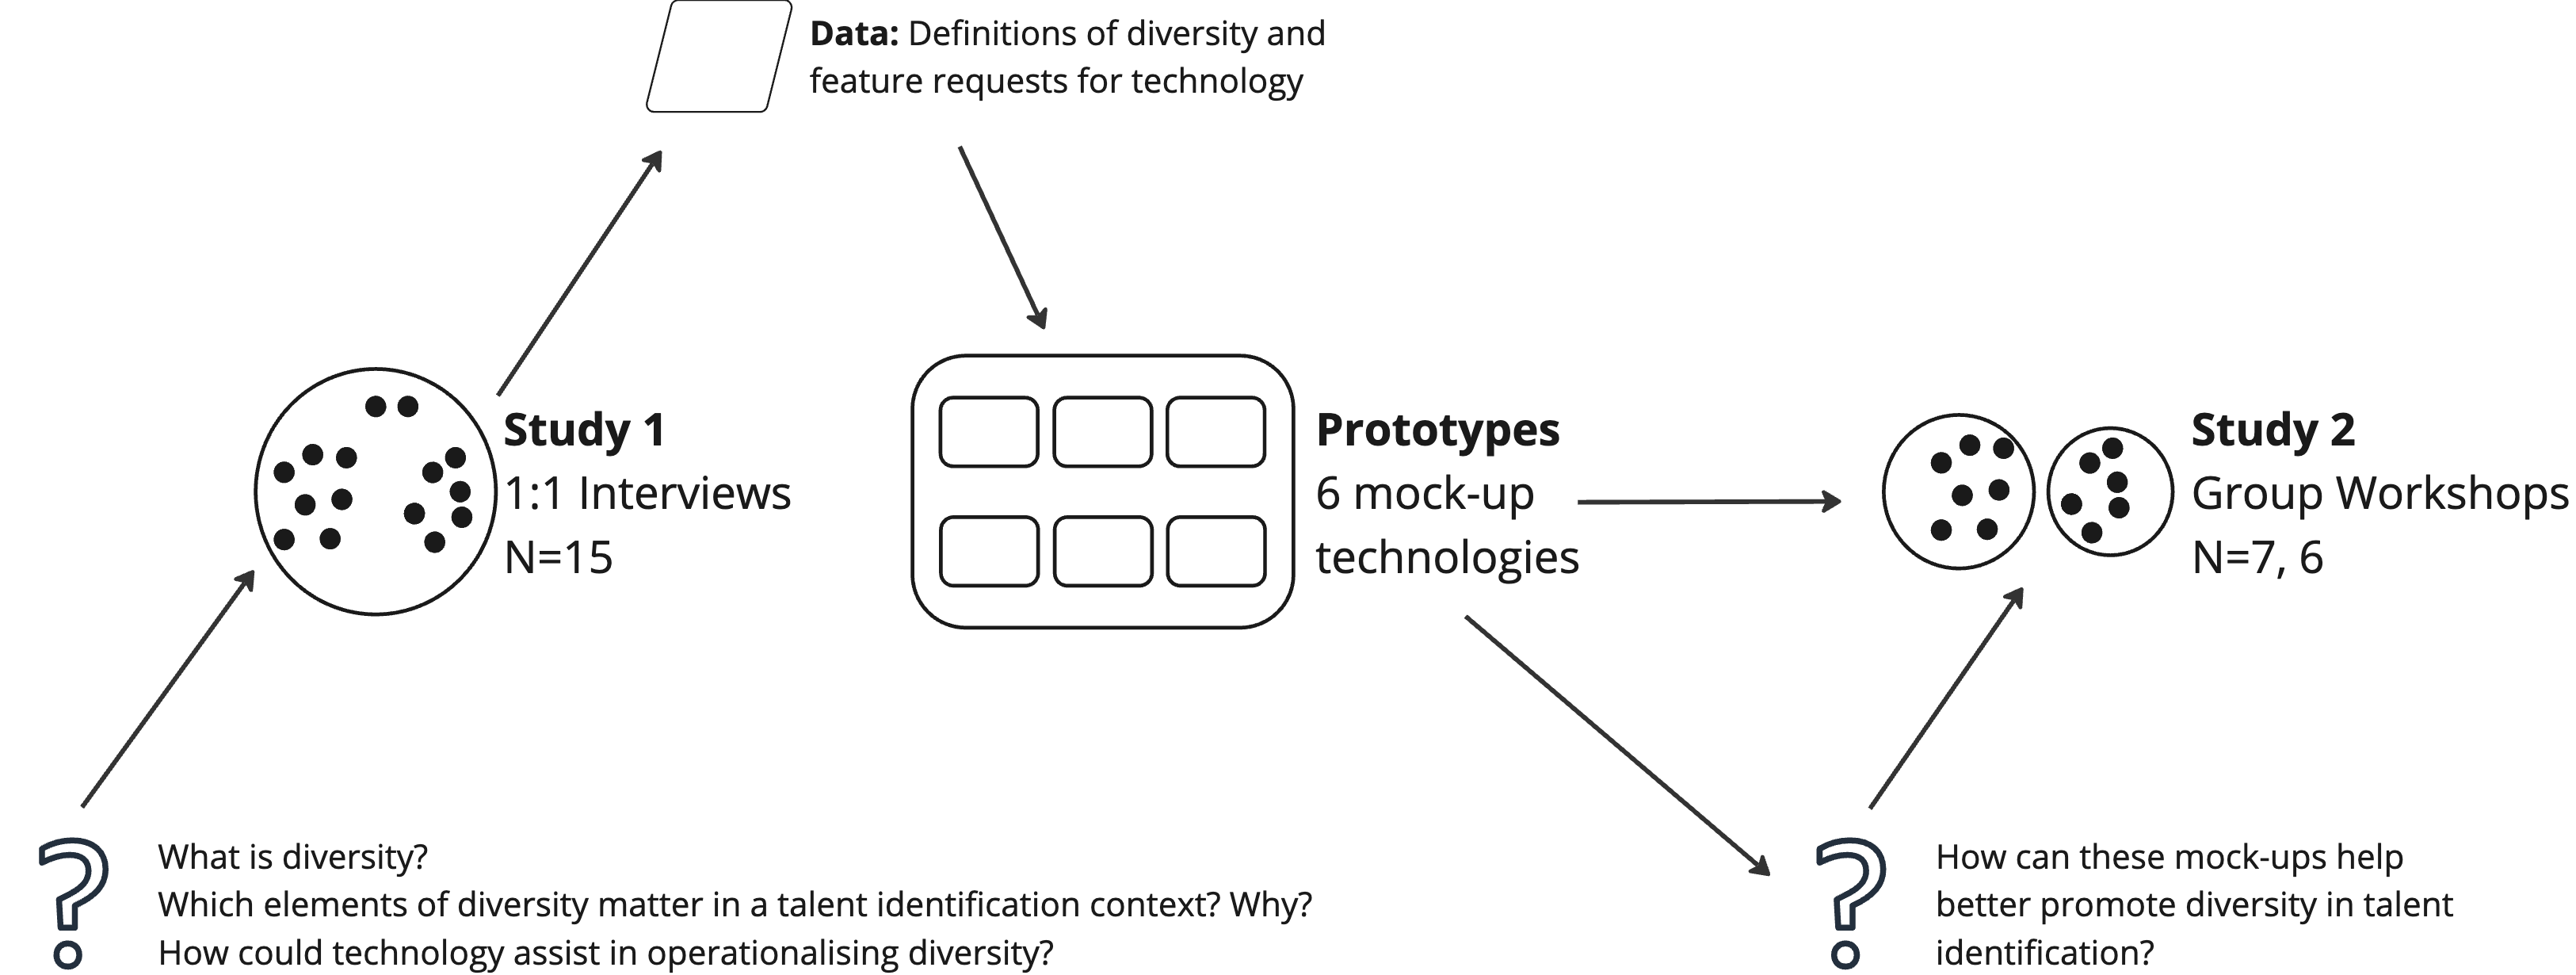
\includegraphics[width=.9\textwidth]{diversity/flowchart.png}
    \caption{This research begins with 15 interviews seeking to understand what selection practitioners mean when they talk about diversity and how to support that, followed with two scenario-speed-dating activities where these practitioners test a number of prototypes built based on the interviews.}
    \label{fig:flowchart}
\end{figure}

In the first session, we seek to ascertain how these practitioners understand diversity, how they operationalise it in processes for selecting talented applicants, and how they envision using technology to assist them in that process. In the second session, we show these practitioners six prototypes built in response to the interviews, then we aim to collaboratively design tools that can help them better consider diversity in selection.

\subsection{Positionality}
Following \textcite{venn-wycherley_realities_2024}, we state researcher positionality here. All authors endorse diversity as a societal and organisational value as discussed in Section \ref{ssec:value} (while sympathetic to the critiques of \textcite{Ahmed_2012,Warikoo_2019}); we thus contend that improving organisational capability to consider diversity is generally a positive development. The research team is comprised of three men and one woman; ethnically, two researchers are South Asian, while two are White; researchers represent three different primary nationalities; all researchers are affiliated with the University of Oxford.

\subsection{Participants}
We engaged selection practitioners (N=15) from two scholarship and talent investment programs. These participants' numbers can be seen in Table \ref{tab:participants}. Where participants participate in the second activity, their groupings for the activities can be seen here as well.

Before either study, we obtained informed consent from all participants to be included in both studies. All participants were given the option to recuse themselves from Study 1 at any point until publication, but, as Study 2 is a group workshop (and as we do not do participant-level attribution), participants were asked to recuse themselves before this second study. Two participants recused themselves before Study 2, but gave leave to be included in Study 1. Participants also gave consent to be recorded, and to have these recordings stored on a secure server. All recording, transcribing, and data analysis was conducted on secure servers. Ethics review was performed by the University of Oxford's Central University Research Ethics Committee.

\begin{center}
\begin{table}[htbp]
    \centering
    \caption{Our fifteen participants are interviewed then split between two groups, with two participants in neither group activity.}
    \label{tab:participants}
    \begin{tabular}{l l l}
        \toprule
        Activity Group 1 (G1) & Activity Group 2 (G2) & No Activity Group (N/A)\\
        \midrule
        P1 & P2 & P8 \\
        P4 & P3 & P12 \\
        P5 & P6 & \\
        P9 & P7 & \\
        P10 & P11 & \\
        P13 & P15 & \\
        P14 & & \\
        \bottomrule
    \end{tabular}
\end{table}
\end{center}

\section{Part 1: Interviews and Thematic Analysis}\label{sec:study1}
\subsection{Methodology}\label{ssec:methods1}
Our interviews aim to answer three questions in each organisational context:

\begin{enumerate}
    \item What is diversity?
    \item Which elements of diversity matter in a selection context? Why?
    \item How could technology assist in operationalising diversity?
\end{enumerate}

In answering our first set of research questions, we follow \textcite{braun_using_2006}'s methodology for reflexive thematic analysis. We first conduct 45-minute semi-structured interviews with 15 selection practitioners. In each interview, we first ask general questions about their selection methodology; we next ask specifically about diversity and its role in selection; we move on to \textcite{Knapp_Zeratzky_Kowitz_2016}'s `crazy 8s' exercise, where participants give eight feature requests in eight minutes; we conclude with a `magic app' exercise inspired by \textcite{blythe2014research}'s design fiction, where participants more thoroughly detail their ideal app. A question-by-question protocol for these interviews is supplied in Appendix \ref{app:divprotocol1}.

The lead author interviewed participants, then transcribed and anonymised the interviews. The lead author and another author (who wasn't present during the interviews) then independently `open-coded' each anonymised transcript to mitigate bias, looking for anything relevant to our research questions. The researchers met six times to discuss their open codes, then shared these codes with the remainder of their research team across four meetings; the researchers grouped codes into 6 themes and 18 subthemes after consensus was reached. These themes are detailed in Table \ref{tab:themes} and described in Section \ref{ssec:themes}.

\begin{table}[htbp]
    \centering
    \caption{Our three central subthemes all speak to the question ``why diversity?''. Other themes and subthemes reflect types of diversity, concepts intertwined with diversity, and other considerations scholarship programs must weigh against diversity desires.}
    \label{tab:themes}
    \begin{tabular}{|p{0.45\textwidth}|p{0.45\textwidth}|}
        \hline
        \multicolumn{2}{|c|}{\textbf{Themes and Subthemes}} \\
        \hline
        \textbf{Why Diversity?} & \textbf{Types of Diversity} \\
        \underline{Different perspectives} & \underline{Socioeconomic} \\
        \emph{...in the same room} & \emph{parental income} \\
        \underline{Representativeness} & \emph{parental education} \\
        \emph{...of a general population} & \emph{generational wealth} \\
        \emph{...of the eligible population} & \underline{Sex, gender, and sexuality} \\
        \emph{...of the applicant population} & \emph{sex} \\
        \emph{...of a target population} & \emph{gender identity} \\
        \underline{Contextualising applications} & \emph{sexual orientation} \\
         & \underline{Geography} \\
         & \emph{nationality} \\
         & \emph{the `Global South'} \\
         & \emph{region} \\
         & \underline{Race} \\
         & \emph{international categorisations of race} \\
         & \underline{Types of thinking} \\
         & \emph{subject area interest} \\
         & \emph{personality type} \\
         & \emph{core beliefs} \\
         & \emph{problem solving approaches} \\
         & \emph{political views} \\
        \hline
        \textbf{Operational Risks and Considerations} & \textbf{Fairness and Bias} \\
        \underline{Outreach} & \underline{Fairness} \\
        \underline{Support} & \emph{...to the applicants} \\
        \emph{...during the application process} & \emph{...to the world} \\
        \emph{...after selection} & \underline{Bias} \\
        \underline{Selectors} & \emph{measurement bias} \\
        \underline{Applicant fraud} & \emph{decision-makers' bias (prejudicial)} \\
         & \emph{decision-makers' unique perspective (probative)} \\
        \hline
        \textbf{Scholarship Goals} & \textbf{Merit} \\
        \underline{Impact} & \underline{Performance relative to disadvantage} \\
        \emph{...on all applicants} & \underline{Measurement} \\
        \emph{...on the selected scholars' performance} & \underline{Performance} \\
        \emph{...on the selected scholars' opportunities} & \\
        \emph{...by the selected scholars on the world} & \\
        \hline
    \end{tabular}
\end{table}

\subsection{Themes}\label{ssec:themes}
\subsubsection{Why Diversity}
A central theme of our investigation revolved around the question of why diversity matters. To this end, we asked questions such as: ``What is diversity?'' and ``Why does diversity matter?''. Answers to: ``What is diversity?'' are visualised in Figure \ref{fig:diversity_is_teaser}; as hypothesised, these answers are vague and uninformative. Interestingly, though, answers to: ``Why does diversity matter?'' informed more specific definitions. We were able to cluster these more specific definitions into three central subthemes: `different perspectives', `representativeness', and `contextualising applications'. These are listed as subthemes of `Why Diversity' in Table \ref{tab:themes}.

\paragraph{Different Perspectives}
8 out of 15 participants mentioned that diversity was important because it brought different perspectives into the same room. This was seen as important for a few related reasons, e.g., the ability to see problems from different angles and the ability to make better decisions. Several participants referred to the: ``Benefits of diverse perspectives'' (P1). One said, when discussing their personal experience working with winners in a talent investment program, that there is: ``Magic happening with lots of...diverse perspectives in the room'' (P14). Peoples' experiences were particularly relevant here. As one participant writes: ``You want to have diverse perspectives from people who look different with different experiences'' (P2).

\paragraph{Representativeness}
9 out of 15 participants spoke of `representativeness'. This, we observed, was often spoken of in relationship to a larger population. Most frequently, participants spoke of the importance of having a cohort that was representative of the `eligible population'. I.e., one participant said: ``[You want] a community which is representative of where you are selecting young people from'' (P6). Others spoke of this in broader, more general terms: ``[You want] as broad a range of people as possible'' (P15). Participants identified the importance of building a cohort that variously: ``Reflects the population of the countries'' (P15) and is ``More representative of the national population than the STEM field already is'' (P10). Others talk about representation of a particular target population, i.e.: ``Representation...because that gives you insight for the people that you're trying to serve....you have to be....reflective of your market'' (P9). Finally, selectors discussed the importance of representing an applicant population: ``[We want] a cohort that is representative of the pool'' (P10).

\paragraph{Contextualising Applications}
`Contextualising applications' was often spoken of by 6 out of 15 participants, most often in individual terms, speaking of identifying particular applicants in need of support, then offering them a `boost' in the form of said support. I.e.: ``Identify those talents and specifically boost up people who are in need of support'' (P5). One participant identified `boosting' as a key metric for the programme: ``We need to know that...we have some level of...impact here, and...if all we're doing is supporting someone who is already on an amazing trajectory and then maybe that means we're not altering their trajectory at all. That's a question of efficiency of our dollars'' (P8).

In some cases, the need for support or boosting was identified with underrepresented or disadvantaged demographic groups. One participant said: ``The focus on gender has been to give the sex that has had the least opportunity the opportunity in this program'' (P9).

\subsubsection{Types of Diversity}
Another central focus of our investigation was on different types of diversity. We asked participants to break down their understanding of diversity into different elements, and to discuss why these elements were important. We found that participants identified a wide range of different types of diversity, which we clustered into subthemes. These subthemes are listed as subthemes of `Types of Diversity' in Table \ref{tab:themes}.

Notably, in addition to the standard demographic categories commonly considered `demographic diversity', participants identified a wide range of other types of diversity commonly termed `cognitive diversity' \cite{page_diversity_2010}. These included `subject areas of interest', `personality type', `core beliefs', `problem solving approaches', and `political views'.

\paragraph{Socioeconomic}
All 15 participants identified socioeconomic diversity as particularly important in the context of a talent investment program. One participant said: ``Socioeconomic [diversity] is probably the most important'' (P1). Another said: ``Socioeconomic background is number one from my perspective'' (P5). This was identified as particularly important for several reasons. Participants stated: ``Because right now the SAT, for example, is more highly correlated to socioeconomic status than it is to anything else'' (P5), and: ``It's a scholarship scheme, so I think it should be for kids who cannot afford normally the fees at the university'' (P7).

Outside of the standard categorisations by income and wealth, participants also identified: ``Familial education level'' (P5) or ``Socioeconomic backgrounds'' (P10) as a particularly important metric for understanding socioeconomic diversity in a scholarship context. This suggests that historical socioeconomic status is considered alongside present socioeconomic status. One participant noted that socioeconomic status varied in both meaning and measurement from country to country: ``For example, in Columbia, there's a whole society to organise on a 1 to 7 scale for socioeconomic status'' (P5). (Columbia's policy of socioeconomic stratification divides households into six strata; unlike traditional measurements such as income or quality of life, these strata only consider household location and accommodation and thus capture a different facet of socioeconomic status \cite{CHICAOLMO2020102560}.)

\paragraph{Sex, gender, and sexuality}
While all 15 participants noted some manner of sex, gender, and sexuality diversity as important, participants disagreed on the relative emphasis that should be place on each. One participant noted: ``[Sex] is important. I think it will get diluted if we focus on identity gender because....the purpose of diversity on the gender aspect was to make sure that [men and women] were getting equal opportunities'' (P9). Another noted that, while sexual identification diversity was important in other contexts, they ``Wouldn't select for that'' (P1) in this context. Others listed `sexual orientation' and `gender' as important metrics for understanding diversity in a scholarship context. However, save for the participant who noted the distinction between sex and identity gender, participants expressed reluctance to discuss the relationships between these difficult concepts.

\paragraph{Geography}
14 of the 15 participants mentioned the importance of geography, citing a need for: ``[A] wide array of different geographical...representations'' (P8). Others spoke of a ``Regional distribution'' (P1), which we have included here.

In particular, emphasis was placed on geographic markers of socioeconomic status such as  the `Global South', `indigenous communities', and `low income countries'. One participant noted: ``Immigration status is tied so closely to socioeconomic status'' (P2), while another noted that ``[Geography] is connected to socioeconomics because we know there are some poorer countries and rich countries'' (P7). Others still asked questions like: ``Do they have a passport?....Are they in a refugee camp?'' (P5).

Furthermore, participants saw it as important that their programmes had: ``Global reach'' (P7). They expressed a desire for: ``[A] diversity of people coming from variety of places'' (P7).

\paragraph{Race}
While 11 out of 15 participants identified race as an important dimension of diversity, none suggested they would explicitly select for racial diversity. Several participants instead noted the difficulty of measuring race in a global context: ``Racial categories obviously vary by country'' (P10). One participant noted: ``[In places] like Brazil or England, there are different categories of race than there are in the US...[In Brazil] there's a board of people who decide what people's race are'' (P5). In a global context, however, many participants pointed to relationships between geography and race, and hence suggested diversifying across geography in place of race: ``If it's an international programme then you can use geography as a proxy'' (P5).

\paragraph{Types of Thinking}
4 out of 15 participants discussed a diversity in the types of thinking exhibited by applicants. One participant noted that: ``You want as much representation from different different types of thinking as you can, because I want perspectives to be listened to equally'' (P2). This manifested in many ways.

Participants tended to express the belief that personality-type-diversity could improve group cohesion: ``With that understanding [of] personality types...be able to tell which...people would get on well with each other'' (P14). One participant suggested a ``Personality test'' (P12), and another specifically mentioned a desire to diversify across ``Openness'' (P2).

However, while personality type was seen as important, core beliefs were seen as even more so. One participant noted an interest in diversity of ``Interests politically'' (P12), and expressed a desire for diversity of ``People's core beliefs...separate from religion'' (P12). Another also noted: ``I would try to have a good representation of...religious groups'' (P3).

\subsubsection{Operational Risks and Considerations}
While our study did not focus on the operational aspects of selection, several selectors' understanding of diversity was closely tied to the operational realities of selecting for and running a scholarship. In answering our questions, several participants identified operational risks or considerations that impacted their understanding of diversity. These are listed as subthemes of `Operational Risks and Considerations' in Table \ref{tab:themes}.

\paragraph{Outreach}
While our study was focused primarily on selecting a diverse cohort from a fixed applicant pool, 6 out of 15 participants answered questions from the perspective of outreach with the goal of growing a more diverse pool of applicants to select from. In particular, participants suggested that ``Using technology for....targeted outreach'' (P4) could help improve overall cohort diversity before selection even begins. One said: ``Giving you very clear signposting on where you may want to focus, you know further recruitment or outreach or whatever it might be to make sure that your programme is diverse at the end of the day'' (P6). Another added: ``You can target your outreach dollars to communities where you know that underrepresented talent exists'' (P10).

\paragraph{Support}
Similarly, 8 out of 15 participants suggested that technology could enable the support of applicants from underrepresented groups, which would also improve diversity. One participant suggested that technology could be used to provide: ``[Support] to keep people that you're attracting from underrepresented backgrounds and help them get across the the finish line'' (P10). Participants focused on the: ``Support needed to actually get [applicants] through your programme'' (P10), i.e., supporting applicants after acceptance. Another suggested that technology could be used to provide support to applicants ``After selection'' (P15).

\paragraph{Selectors}
4 out of 15 participants noted that diversity did not apply merely to applicants. Instead, for programs where a group of selectors assists in the selection process, ``Tracking the diversity of the selectors'' (P15) and ``[Monitoring] how they're scoring and reviewing applicants [for] prejudice or biases'' (P15).

\paragraph{Applicant fraud}
Finally, only 2 out of 15 participants expressed concern with selecting based on particular diversity characteristics, especially self-reported metrics of diversity characteristics, was the potential for applicant fraud, e.g. falsely reporting demographic or other attributes with the aim of increasing their chances of acceptance. One participant requested: ``A fraud detector'' (P5), while another expressed a desire to ensure that the process ``Isn't super gameable'' (P10).

\subsubsection{Fairness and Bias}
Though not a type of diversity as we have understood it here, many participants referenced similarities between diversity metrics and metrics of fairness or bias (as in \textcite{zhao2023fairness}). Furthermore, several suggested that improving fairness while reducing bias would likely yield a more diverse cohort. These themes are reflected under `Fairness and Bias' in Table \ref{tab:themes}.

\paragraph{Fairness}
6 out of 15 participants discussed that it was important that applicants: ``Get fair chance on their on their academic merit'' (P7). This translated to an emphasis on ``Fairness in the assessment'' (P7).

However, participants also noted that ``The way the world works is unfair'' (P14), and found it important that the programme is: ``Making sure that the world is fairer by bringing more diversity to this world'' (P7). In this way, participants found: ``[The] representative thing....goes back to fairness'' (P15). One participant noted that: ``Affirmative action....can come across as unfair to some people, but....it's trying to balance things out when things have been so unequal for so long'' (P3). This supports \textcite{zhao2023fairness}'s positioning of fairness as related to, rather than in opposition to, diversity. 

\paragraph{Bias}
11 out of 15 participants discussed bias, often as both a human- and machine-decision-making problem. Many participants appealed to technology's ability to be comparatively impartial as an important mitigator of bias, i.e., one participant repeatedly requested a: ``Non-biased program'' (P3); another stated a preference for: ``Data analysis to make decisions on who we should be supporting as opposed to having humans try to make those decisions with all their biases'' (P5). However, those same participants noted that common machine decision-making paradigms amplify bias, and that it was important to be aware of this: ``AI has a lot of bias in it'' (P3).

Others noted the possibility for technology to elucidate biases in both humans and machines. One participant requested: ``Some kind of tool that can detect bias in a selection'' (P7).

\subsubsection{Programme Goals}
Selection practitioners from both programmes identified goals for their programmes. These goals were discussed by both groups as an intended form of `impact' and both groups closely related achieving their goals to their expressions of why diversity mattered. While impact goals vary based on the type of impact and the affected party, we discuss these as `impact' in Table \ref{tab:themes}.

\paragraph{Impact}
5 out of 15 participants found key goals of their program to include: ``Orient[ing] [scholars] towards social impact or using their talent for good'' (P8). They tended to encourage: ``[Scholars'] working towards something impactful over the course of their career'' (P8).

\subsubsection{Merit}
Several participants reflected on the relationship between merit and diversity. While some participants saw these as competing goals, others saw them as complementary. In particular, complementary views often viewed merit as a form of performance relative to specific advantages, or noted that many of our measurement tools are biased across our chosen diversity dimensions. These themes are reflected as subthemes of `Merit' in Table \ref{tab:themes}.

\paragraph{Performance relative to disadvantage}
2 out of 15 participants identified merit as something difficult to disentangle from performance. One participant noted that applicants may appear less qualified because they: ``Didn't have the chance; didn't have the opportunities'' (P2), while others with the opportunities will appear more qualified. Another participant began by asking: ``How good is their three A stars based on where they've come from?'' (P12), then proceeded to reflect that ``Your performance relative to your opportunity or maybe expected performance'' (P12) is a key indicator of merit.

\paragraph{Measurement}
Closely related, 3 out of 15 participants questioned our ability to measure merit independent of opportunity: ``[Whether they perform well] because they have the opportunity or because they are brilliant – I think that these two are really difficult to untangle'' (P7). Another noted that: ``Contextual factors mess up our otherwise seemingly objective measures of merit.... national context and family income is messing up your ability to measure the thing you actually care about'' (P10). They continued to note that they: ``Need to pay attention to [diversity] because it's messing up your measures of what you actually care about'' (P10).

\paragraph{Performance}
Finally, 2 out of 15 participants noted occasions where performance and diversity were ostensibly competing goals. However, even here, participants recognised that observed performance and actual merit may differ. One participant noted that: ``[The] overriding aim is for [the programme] to be as diverse as is possible but still meet a standard....relative score of like how good their application is based on all these kind of contextual factors'' (P12). Another requested a technology that helps discover how: ``Close you are to your idealised diversity targets and how close you are to maximising whatever it is you think you're maximising in your performance scores'' (P10).

\section{Part 2: Participatory Design}\label{sec:study2}
\subsection{Prototypes}
As a next step, we applied the results of our thematic analysis to design six prototypes following methodology from \textcite{Buchenau_Suri_2000}. These technologies aimed to help selection practitioners better understand and operationalise diversity in their selection processes. We then present these prototypes to participants in participatory design workshops. These prototypes are shown in Figure \ref{fig:prototypes}.

Three of these prototypes (Figures \ref{fig:representativeness}, \ref{fig:entropy}, and \ref{fig:diversity}) present information about the range of possible cohorts participants must choose between, while the other three (Figures \ref{fig:demographic}, \ref{fig:impact}, and \ref{fig:advantage}) present information about an individual applicant relative to a given cohort and a given pool. Furthermore, five of the six prototypes were designed to satisfy definitions of diversity uncovered in Section \ref{sec:study1}.

\begin{figure}[htbp]
    \centering
    \begin{subfigure}[b]{0.3\textwidth}
        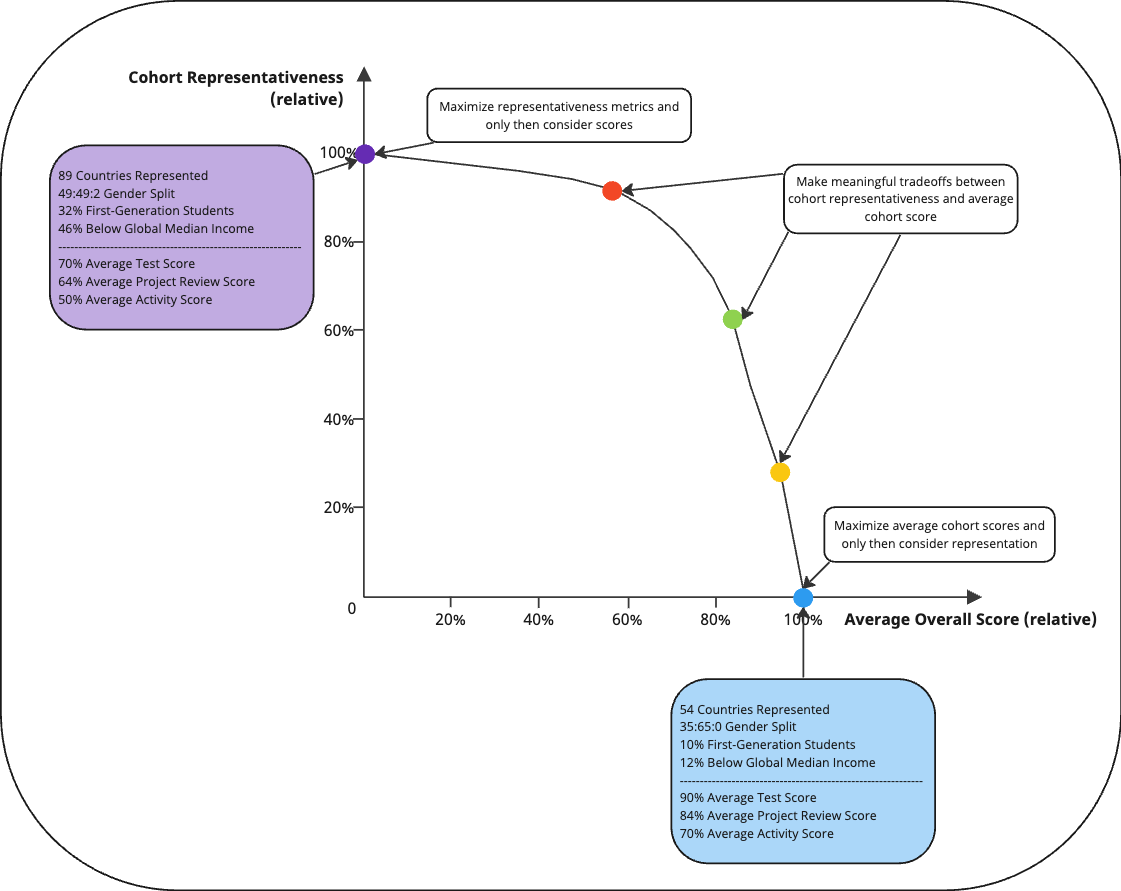
\includegraphics[width=\textwidth]{diversity/representativeness.png}
        \caption{Prototype \ref{fig:representativeness}: Cohort Representativeness}
        \label{fig:representativeness}
    \end{subfigure}
    \hfill
    \begin{subfigure}[b]{0.3\textwidth}
        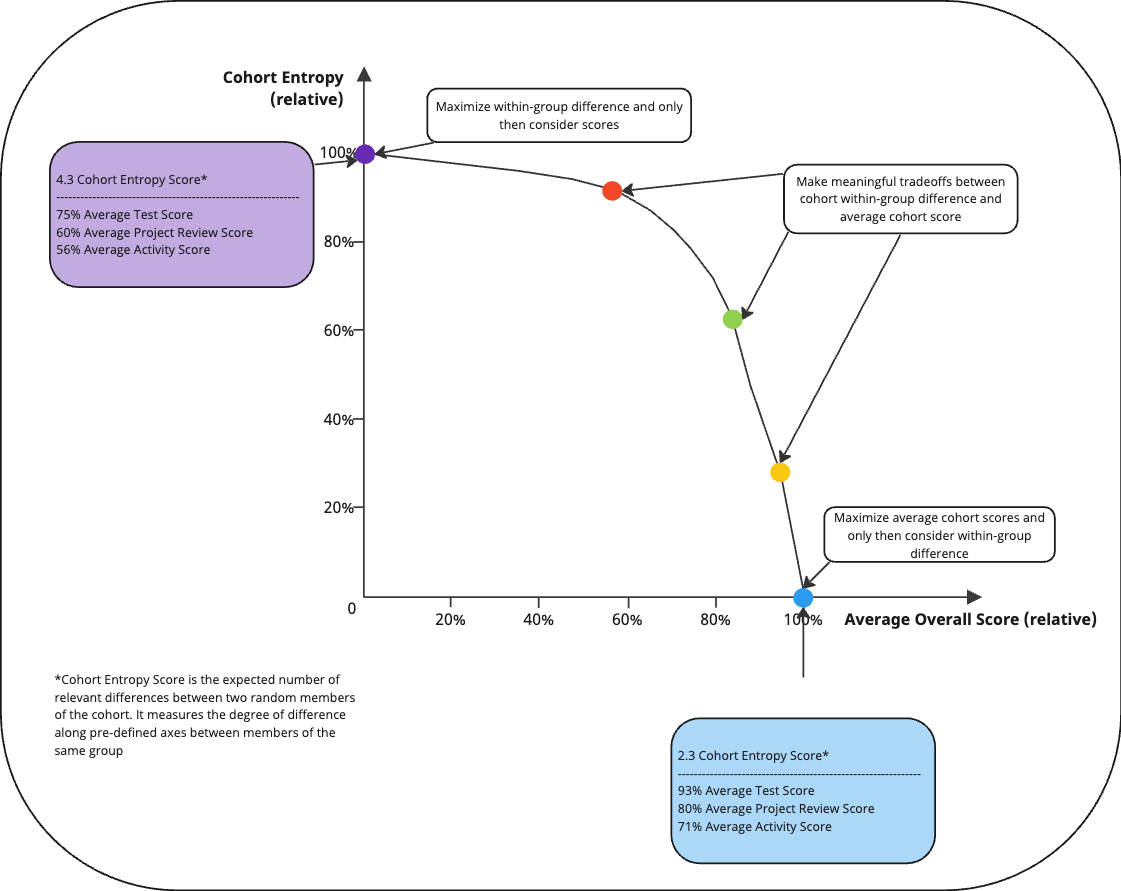
\includegraphics[width=\textwidth]{diversity/entropy.png}
        \caption{Prototype \ref{fig:entropy}: Cohort Entropy}
        \label{fig:entropy}
    \end{subfigure}
    \hfill
    \begin{subfigure}[b]{0.3\textwidth}
        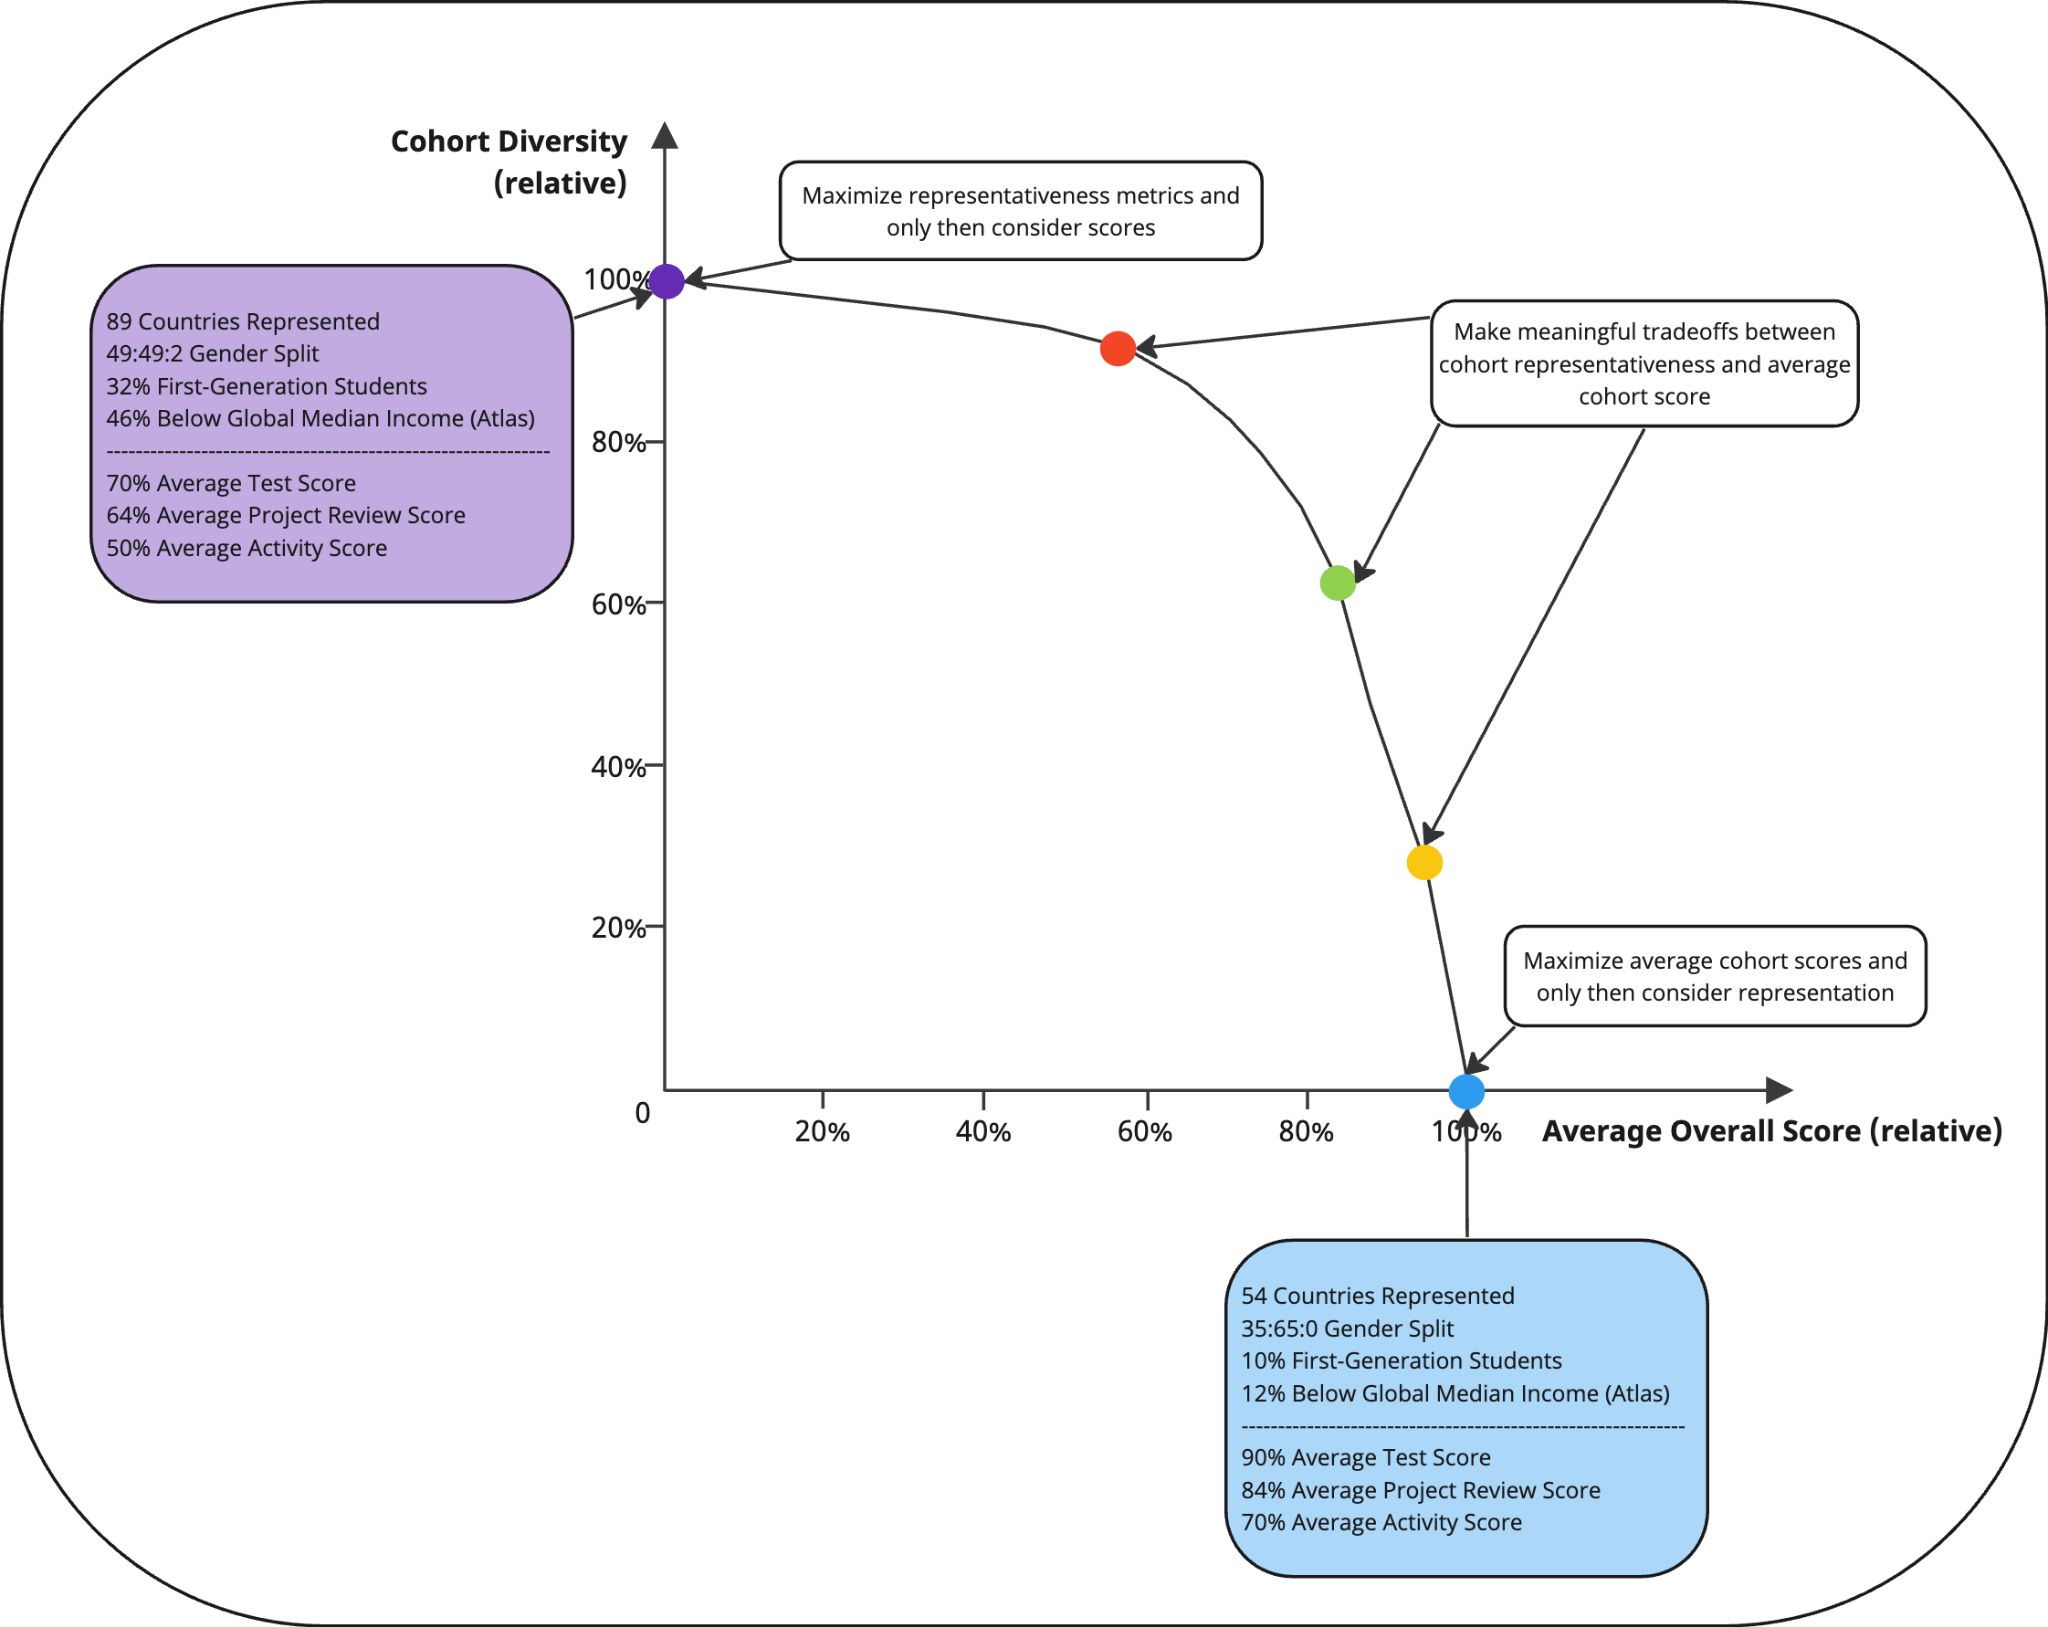
\includegraphics[width=\textwidth]{diversity/diversity.png}
        \caption{Prototype \ref{fig:diversity}: Cohort Diversity}
        \label{fig:diversity}
    \end{subfigure}

    \medskip

    \begin{subfigure}[b]{0.3\textwidth}
        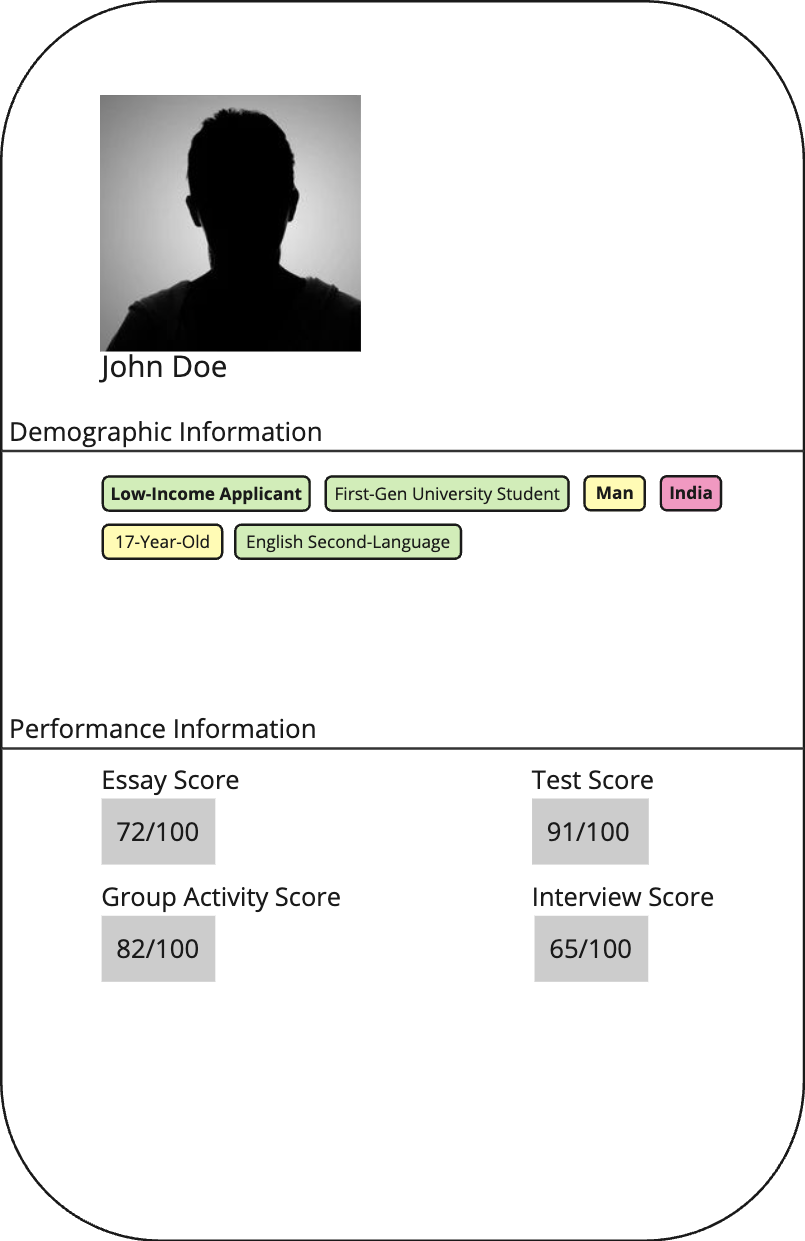
\includegraphics[width=\textwidth]{diversity/demographic.png}
        \caption{Prototype \ref{fig:demographic}: Applicant Demographic Information}
        \label{fig:demographic}
    \end{subfigure}
    \hfill
    \begin{subfigure}[b]{0.3\textwidth}
        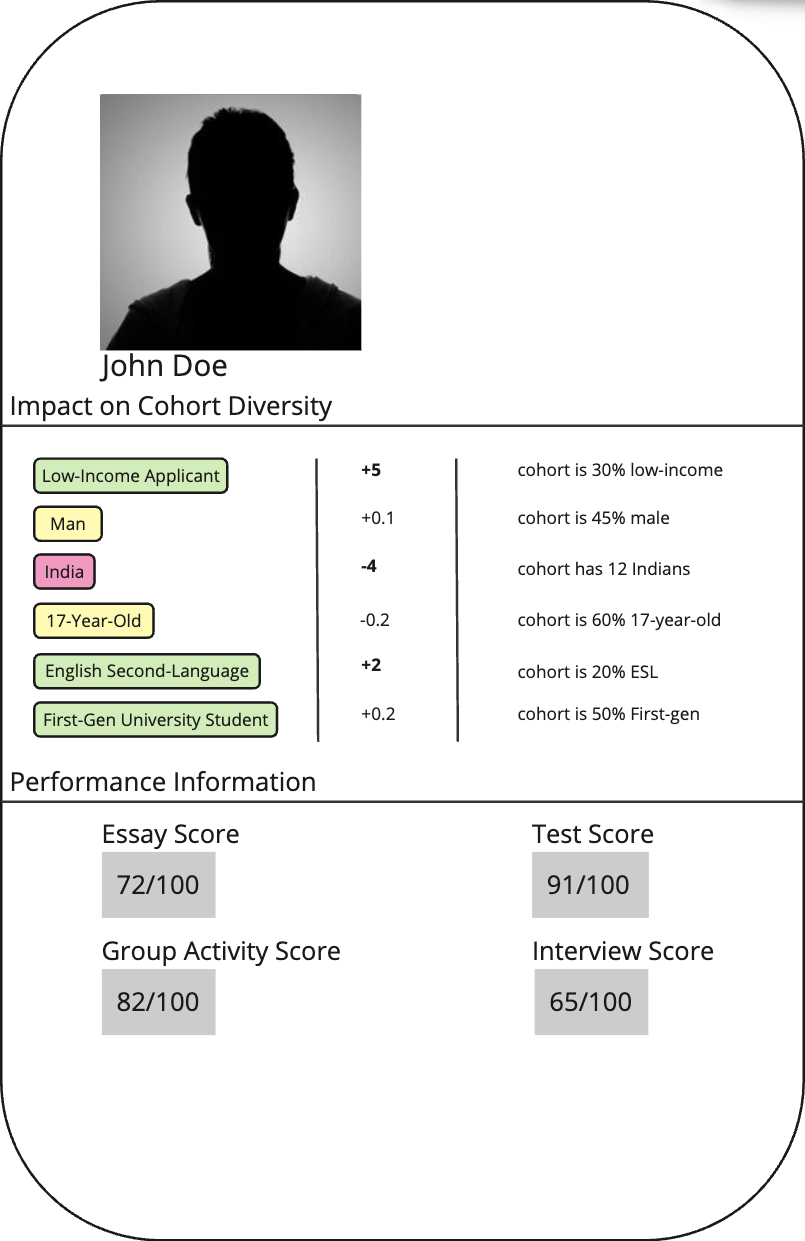
\includegraphics[width=\textwidth]{diversity/impact.png}
        \caption{Prototype \ref{fig:impact}: Applicant Demographic Impact on Cohort}
        \label{fig:impact}
    \end{subfigure}
    \hfill
    \begin{subfigure}[b]{0.3\textwidth}
        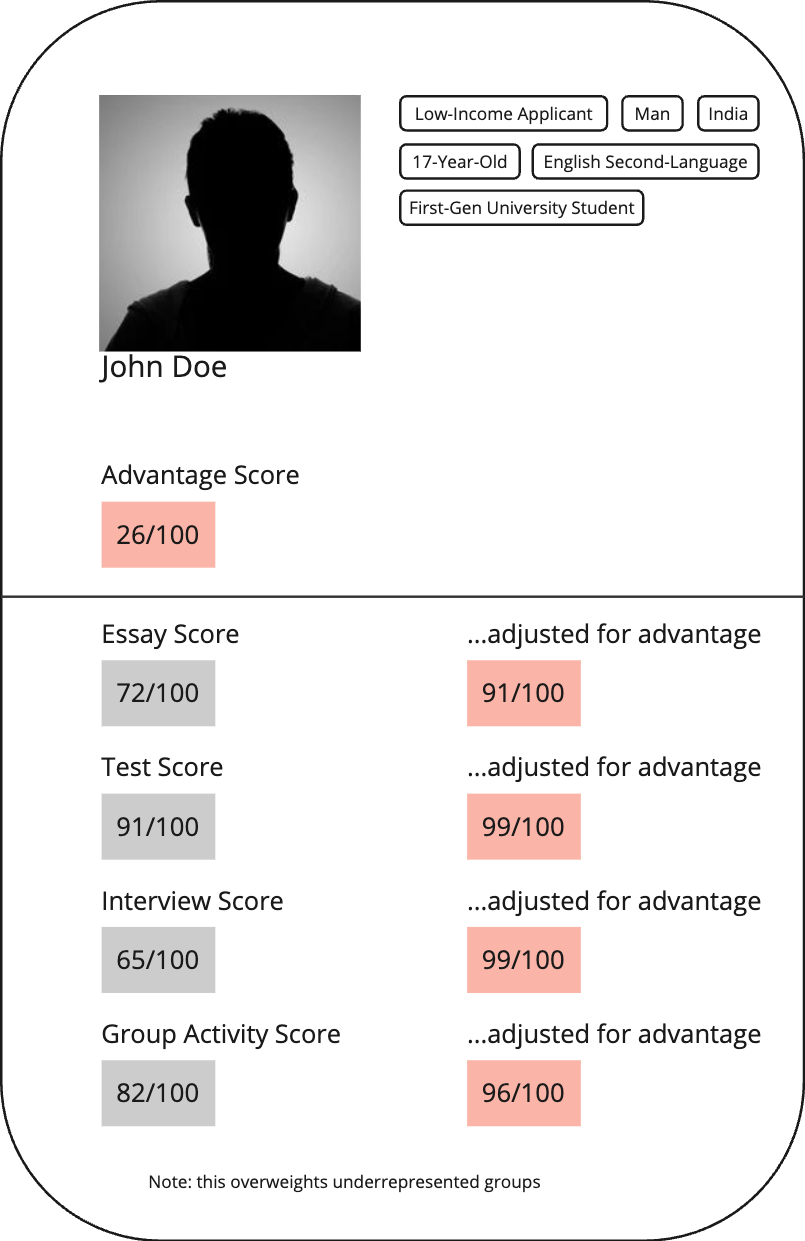
\includegraphics[width=\textwidth]{diversity/advantage.png}
        \caption{Prototype \ref{fig:advantage}: Applicant Advantage Scores}
        \label{fig:advantage}
    \end{subfigure}
    \caption{These figures depict the prototypes designed based on themes from Section \ref{sec:study1} and used in our participatory design workshops. They are reproduced at a larger scale in Appendix \ref{app:figures}}
    \label{fig:prototypes}
\end{figure}

Figures \ref{fig:demographic} and \ref{fig:impact} are based on the `representativeness' theme, while Figure \ref{fig:advantage} is based on the `contextualising applications' theme. Similarly, Figures \ref{fig:representativeness} and \ref{fig:entropy} draw a distinction in their measurements of diversity, based on the `representativeness' and the `different perspectives' themes, respectively. Figure \ref{fig:entropy}, in particular, defines and employs `entropy' as a metric. This reflects that, when aiming to get different perspectives in the same room, the goal is not to represent any target population; rather, we desire that everyone in our group be as different from the remainder of the group as possible.

\subsection{Workshop Methodology}\label{ssec:methods2}
As the participants all come from two separate talent investment programs, we run one workshop for each group \cite{Buchenau_Suri_2000}. Before presenting to the broad audience of each group, we submit our figures to one primary contact (also a participant in the study) at each organisation, then run informal, 15-minute `pilot' one-on-one workshops with this primary contact. Here, we primarily sought approval to use these figures in workshop with the broader team of practitioners, but we also collected minor feedback and tweaked the prototypes based on this feedback. In one organisation's pilot workshop, the primary contact requested Figures \ref{fig:representativeness} and \ref{fig:entropy} be combined into one prototype with `Diversity' as the Y-axis, as the organisation already has an internal working definition of diversity (that aligns very closely with what we mean by representativeness). This can be seen in Figure \ref{fig:diversity}. Participant grouping for the workshops can be seen in Table \ref{tab:participants}; the results for this analysis are attributed by group, rather than individual, to reflect the cooperative nature of the task.

Our central research questions for this workshop are:

\begin{enumerate}
    \item What prototypes best promote diversity?
    \item What elements of these prototypes facilitate their success?
\end{enumerate}

\noindent Or, for each prototype: ``How and why does this prototype promote diversity?''. In each workshop, we ask participants to consider each prototype in turn, and to discuss how they might use it in their selection process. We then ask participants to consider how these prototypes might fit into their current selection process, and how they might change their process to better incorporate these prototypes. Finally, we ask participants to consider how their current selection process might make best use of these prototypes, and whether they think these prototypes would be beneficial. 

Following the methodology of \textcite{Gatian_1994,Griffiths_Johnson_Hartley_2007}, at the end of each workshop, we ask participants to highlight their favourite prototype.

A question-by-question protocol for these workshops can be found in Appendix \ref{app:divprotocol2}.

\subsection{Results}\label{ssec:results2}
\subsubsection{Participants Preferred Prototype \ref{fig:impact}}
As part of the workshop, participants were asked to mark their favourite prototypes \cite{Gatian_1994,Griffiths_Johnson_Hartley_2007}. These favourites have been collated in Table \ref{tab:favourites}, and it can be seen here that Prototype \ref{fig:impact} was by-far the favourite in both groups.

\begin{table}[htbp]
    \centering
    \caption{This table tallies the number of participants indicated that a given prototype was their favourite. The overwhelming favourite was prototype 5, which shows an individual applicant's impact on the cohort.}
    \label{tab:favourites}
    \begin{tabular}{lr}
        \toprule
        \textbf{Prototype} & \textbf{Favourites} \\
        \midrule
        Prototype \ref{fig:representativeness} & 1 \\
        Prototype \ref{fig:entropy} & 1 \\
        Prototype \ref{fig:diversity} & 0 \\
        Prototype \ref{fig:demographic} & 1 \\
        Prototype \ref{fig:impact} & 10 \\
        Prototype \ref{fig:advantage} & 0 \\
        \bottomrule
    \end{tabular}
\end{table}

\subsubsection{Both Groups Rely on Idiosyncratic Notions in Selection}
When participants were placed in a practical selection scenario and shown technology prototype information about (hypothetical) applicants, they compared applicants to idiosyncratic profiles that they desired.

When evaluating Prototype \ref{fig:advantage}, G1 used advantage scores to seek out: ``Diamonds in the rough'' (G1), i.e., talented applicants from disadvantaged backgrounds who lacked the polish of their more privileged counterparts.

Prototype \ref{fig:entropy} was initially confusing to G2, as the `entropy' definition used was unfamiliar to the participants: ``Entropy is chaos in chemistry. How does this relate to our usage here?'' (G2). Thus, when interacting with Prototype \ref{fig:entropy}, G2 understood `entropy' to be variety in cognitive skill-set and personality type. In particular, the group sought to ensure that the chosen cohort contain `glue' people, who improve overall cohort cohesion: ``For people working together, it's useful to have someone who is that `glue''' (G2). 

\subsubsection{Organisations and Participants Are Interested in Different Diversities}
When presented with Prototypes \ref{fig:representativeness} and \ref{fig:entropy}, G2 was given the demonstrative definitions of `representativeness' and `entropy' (visible on the prototypes). G2 quickly understood the differences between the figures to be that Prototype \ref{fig:representativeness} sought to support considerations of demographic representativeness, while Prototype \ref{fig:entropy} sought to support placing different perspectives (be they cognitive skill-sets or personality types) in the same room. Participants were then interested to know the relationship between these prototypes in practice: ``If we maximise based on [Prototype \ref{fig:representativeness}] scores, what would the Entropy scores be?'' (G2).

However, though individual participants took great interest in Prototype \ref{fig:representativeness}, G2 ultimately acknowledged that the program was most interested in building a cohort from people with different perspectives to facilitate collaboration: ``For [our] cohorts, [we] want a balance [of personality types] and [we] want them to be collaborative'' (G2). At the same time: ``Let's track but not use [program-specific measure of representativeness]'' (G2).

\subsubsection{Different Tools are Useful at Different Application Stages}
Participants in both groups variously expressed an anxiety about measuring the relevant dimensions. ``What are our metrics and are they reliable?'' (G2) was echoed by several G2 participants. ``If it's all self-report, then we can't do anything with it'' (G1). 

However, both organisations noted that their selection processes involve a variety of stages. Different tools are useful in different stages. When speaking of Prototype \ref{fig:entropy}, one participant said: ``This is better post-interview than it is pre-interview'' (G2), as interviews will collect observational data on many of these characteristics. I.e., while certain tools may rely on measurements that cannot be collected until later stages, others will be more useful earlier in the selection process.

Similarly, different output modes were useful at different stages. Note that Prototypes \ref{fig:demographic} and \ref{fig:impact} contain similar information, but that Prototype \ref{fig:impact} displays this information in greater detail. When reviewing both prototypes, G1 found Prototype \ref{fig:demographic} preferable in the earlier stages of decision-making, while Prototype \ref{fig:impact} had the greatest utility later. ``[We] can't send [Prototype \ref{fig:impact}] as a pre-read, but [Prototype \ref{fig:demographic}] makes more sense in isolation, so better for a pre-read'' (G1). On Prototype \ref{fig:demographic} in particular, one participant noted: ``Helpful for the process, not so much for the [final cohort selection]'' (G1). Another said of Prototype \ref{fig:impact}: ``This has the most potential at the later stages of decision-making'' (G1).

At the other extreme, while the cohort-level tools did not spark discussions about particular individuals, they did spark earlier-stage, higher-level discussions. Most obviously, both programs discussed specific tradeoffs between measured individual applicant aptitude and cohort diversity: ``Real decision-making always sees tradeoffs like these.... This chart helps you figure out the level of compromise you're willing to make on both axes'' (G2); ``[It] makes sense that top scoring candidates don't necessarily help you build the most diverse cohort.... 5-10\% [of the cohort] really get to a struggle between quality and diversity.... If this chart were real (rather than hypothetical), and you could see who you were losing, this would be useful'' (G1). (In the hypothetical,  participants from G1 settled closer to the centre of the frontier: ``[Our] target here is to look somewhere [from] red to yellow'' (G1). However, they also noted that ``Some candidates get a big diversity boost and score terribly'' (G1).)

In one case, participants also discussed broader, program-level concerns. Participants spent time debating ``Is the program needs-based or merit-based?'' (G1). They noted  that ``This chart helps [facilitate that discussion]'' (G1), but did not ultimately conclude one way or the other.

\subsubsection{The Right Balance of Quantitative and Qualitative Information is Key}
Participants simultaneously expressed gratitude that the prototypes were as simplified as they were, and a desire for more detail. One participant from G1 noted that the prototypes are: ``Very constrained in terms of what is being shown.... This doesn't include all of the factors, but for the decision that's good, because it prevents info overload'' (G1). However, participants G2 frequently requested additional quantitative information. In the case of the Prototype \ref{fig:impact} (participants' favourite prototype, as can be seen in Table \ref{tab:favourites}), participants requested a number of other metrics: ``Advantage score'' (G2), ``Impact on entropy'' (G2), ``[A summary of] these scores together'' (G2), and ``A composite impact on cohort diversity'' (G2).

Meanwhile, participants from G1 requested qualitative information: ``We need to know more about the applicants' backgrounds'' (G1). Other requested information included: ``Comments from selectors'' (G1) and ``A narrative summary...written by the selector team'' (G1). 

This suggests a discrepancy between the two groups' preference for the balance between qualitative and quantitative information. While G2 expressed a desire for unifying quantitative metrics: ``A single score for disadvantage [or] need, while recognising its flaws, could provide one read of an individual's circumstances'' (G2), G1 expressed a desire for individual, qualitative information: ``We're using quantitative to sift through qualitative.... [We] need to include comments from selectors'' (G1).


\section{Design Recommendations}
\begin{figure}[htbp]
    \centering
    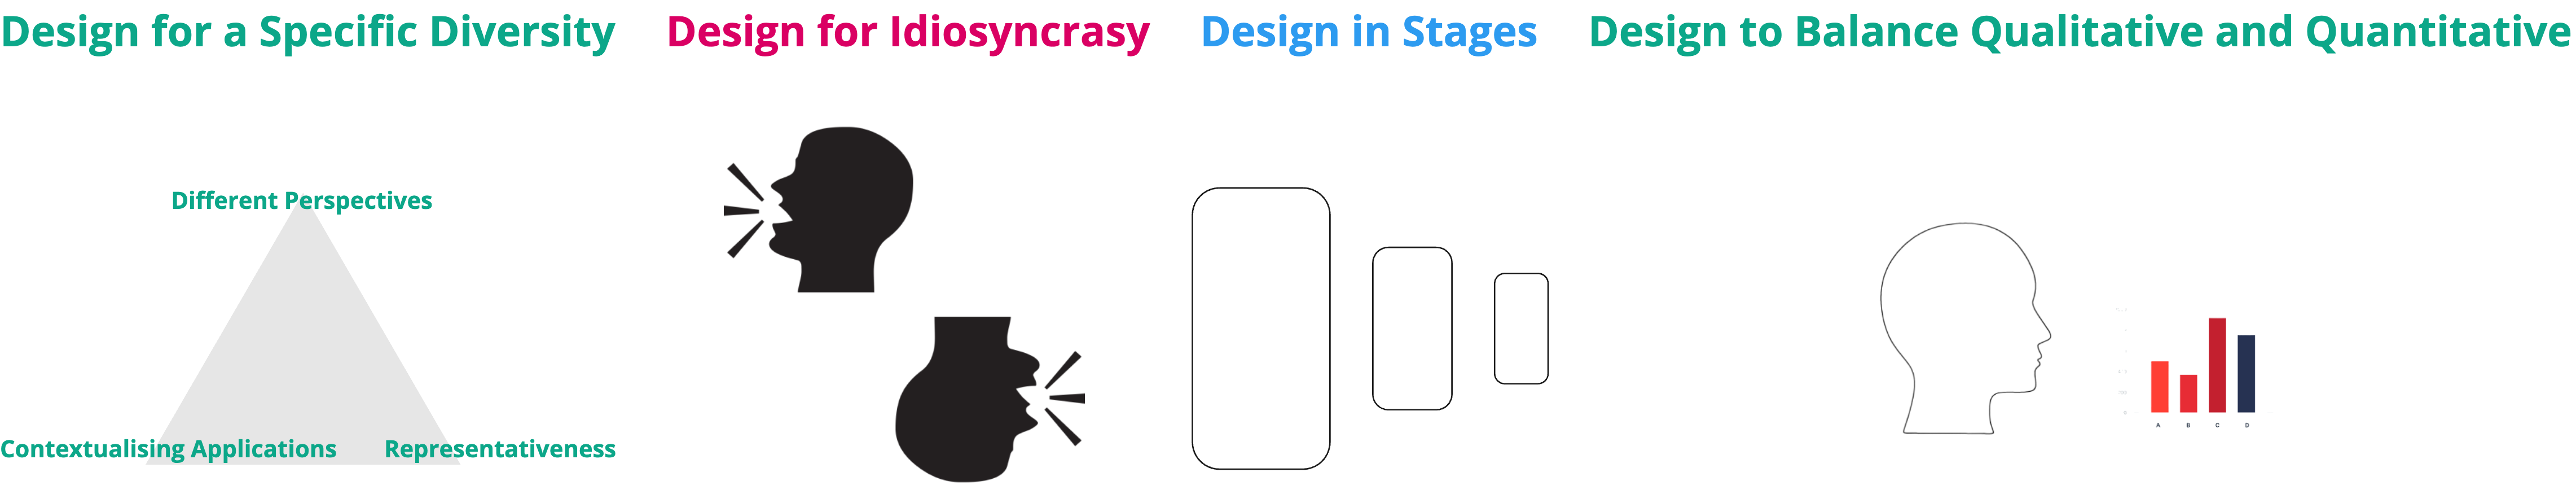
\includegraphics[width=0.9\linewidth]{diversity/recommendations.png}
    \caption{This figure illustrates our four key design recommendations to others building tools to support the selection of diverse talent, i.e., `design...': `...for a specific diversity', `...for idiosyncrasy', `...in stages', and `...to balance qualitative and quantitative'.}
    \label{fig:recommendations}
\end{figure}

\subsection{Design for a Specific Diversity}
In the initial interviews, participants were often vague when asked to define diversity. However, when asked to expand on why diversity is important, or on what dimensions of diversity they prioritised, it became clear that `diversity' included three separate (and sometimes competing) definitions. We have termed these: `representativeness', `different perspectives', and `contextualising applications'. When designing tools to assist a target organisation in considering diversity, we suggest designers first clarify through human-centric methods which definitions of diversity the target organisation seeks to consider, then designs to support those specific definitions. That is, designers should follow \textcite{VanKleek_Seymour_Binns_Shadbolt_2018}'s paradigm of `respectful' design and build technology to best serve the needs of the selection practitioners who will use it.

\subsection{Design for Idiosyncrasy}
One key note revealed through this process is that different decision-making processes have philosophical underpinnings, desiderata, and anecdotal definitions that impact their selections. These idiosyncrasies should be discovered early in development and designed for in any technical solution. We suggest participatory design as a mechanism for achieving this. We observed a strong relationship between participant feedback in interviews and their satisfaction with the prototypes.

For example, both talent investment programs we worked with have created specific personas they look for. For example, one group discussed `glue' people who helped groups function cohesively. The other group discussed `diamonds in the rough', talented youth systemically undervalued due to their backgrounds. Where these aspects were included, participants showed strong interest in the prototypes. Where they were excluded, participants often asked for these to be added.

\subsection{Design in Stages}
Much of what participants desired at one stage of decision-making was mutually exclusive with that they desired at other stages. For example, G1 desired Prototype \ref{fig:demographic} as a: ``Pre-read'' (G1) due to its simplicity, but preferred the detail of Prototype \ref{fig:impact} ``In the room'' (G2). Thus, it is crucial for designers to consider what stage of decision-making their tools are designed to support, and to design appropriate levels of detail, abstraction, and engagement accordingly.

\subsection{Design to Balance Qualitative and Quantitative}
Participants often noted that the prototypes were missing key qualitative information about applicants. This qualitative information is crucial in holistic considerations of each applicant. However, when allowed to consider only qualitative information, participants obscure tradeoffs they are forced to make between different program goals. In particular, while individual-level goals are often clear, cohort-level goals (such as diversity) are easier to delay or ignore. Thus, without quantitative tools to frame the discussion, participants noted that they were often forced to make cohort-level considerations ad-hoc and towards the end of their decision-making process.

Thus, while qualitative information is crucial, it is also important to present the quantitative information necessary to make these tradeoffs salient. Ultimately, final selection decisions are made by panels of trained selectors, but in the absence of both quantitative and qualitative information to guide these decision-makers, they would be forced to make decisions that are less well-informed than they could be.

\section{Discussion}\label{sec:divdisc}
\subsection{The Diversity Triangle}
In Section \ref{sec:study1}, participants variously identified the word `diversity' with three themes, which we have taken to signify definitions of diversity: `representativeness', `different perspectives', and `contextualising applications'. As these three definitions are central to our research questions, we privileged them over Section \ref{sec:study1}'s other themes in Section \ref{sec:study2}, where we engaged in scenario speed dating and experience prototyping designed to satisfy different definitions of diversity. In this section, we map the themes to the three definitions in the \emph{Diversity Triangle} (Figure \ref{fig:div_triangle}).

\begin{figure}[htbp]
    \centering
    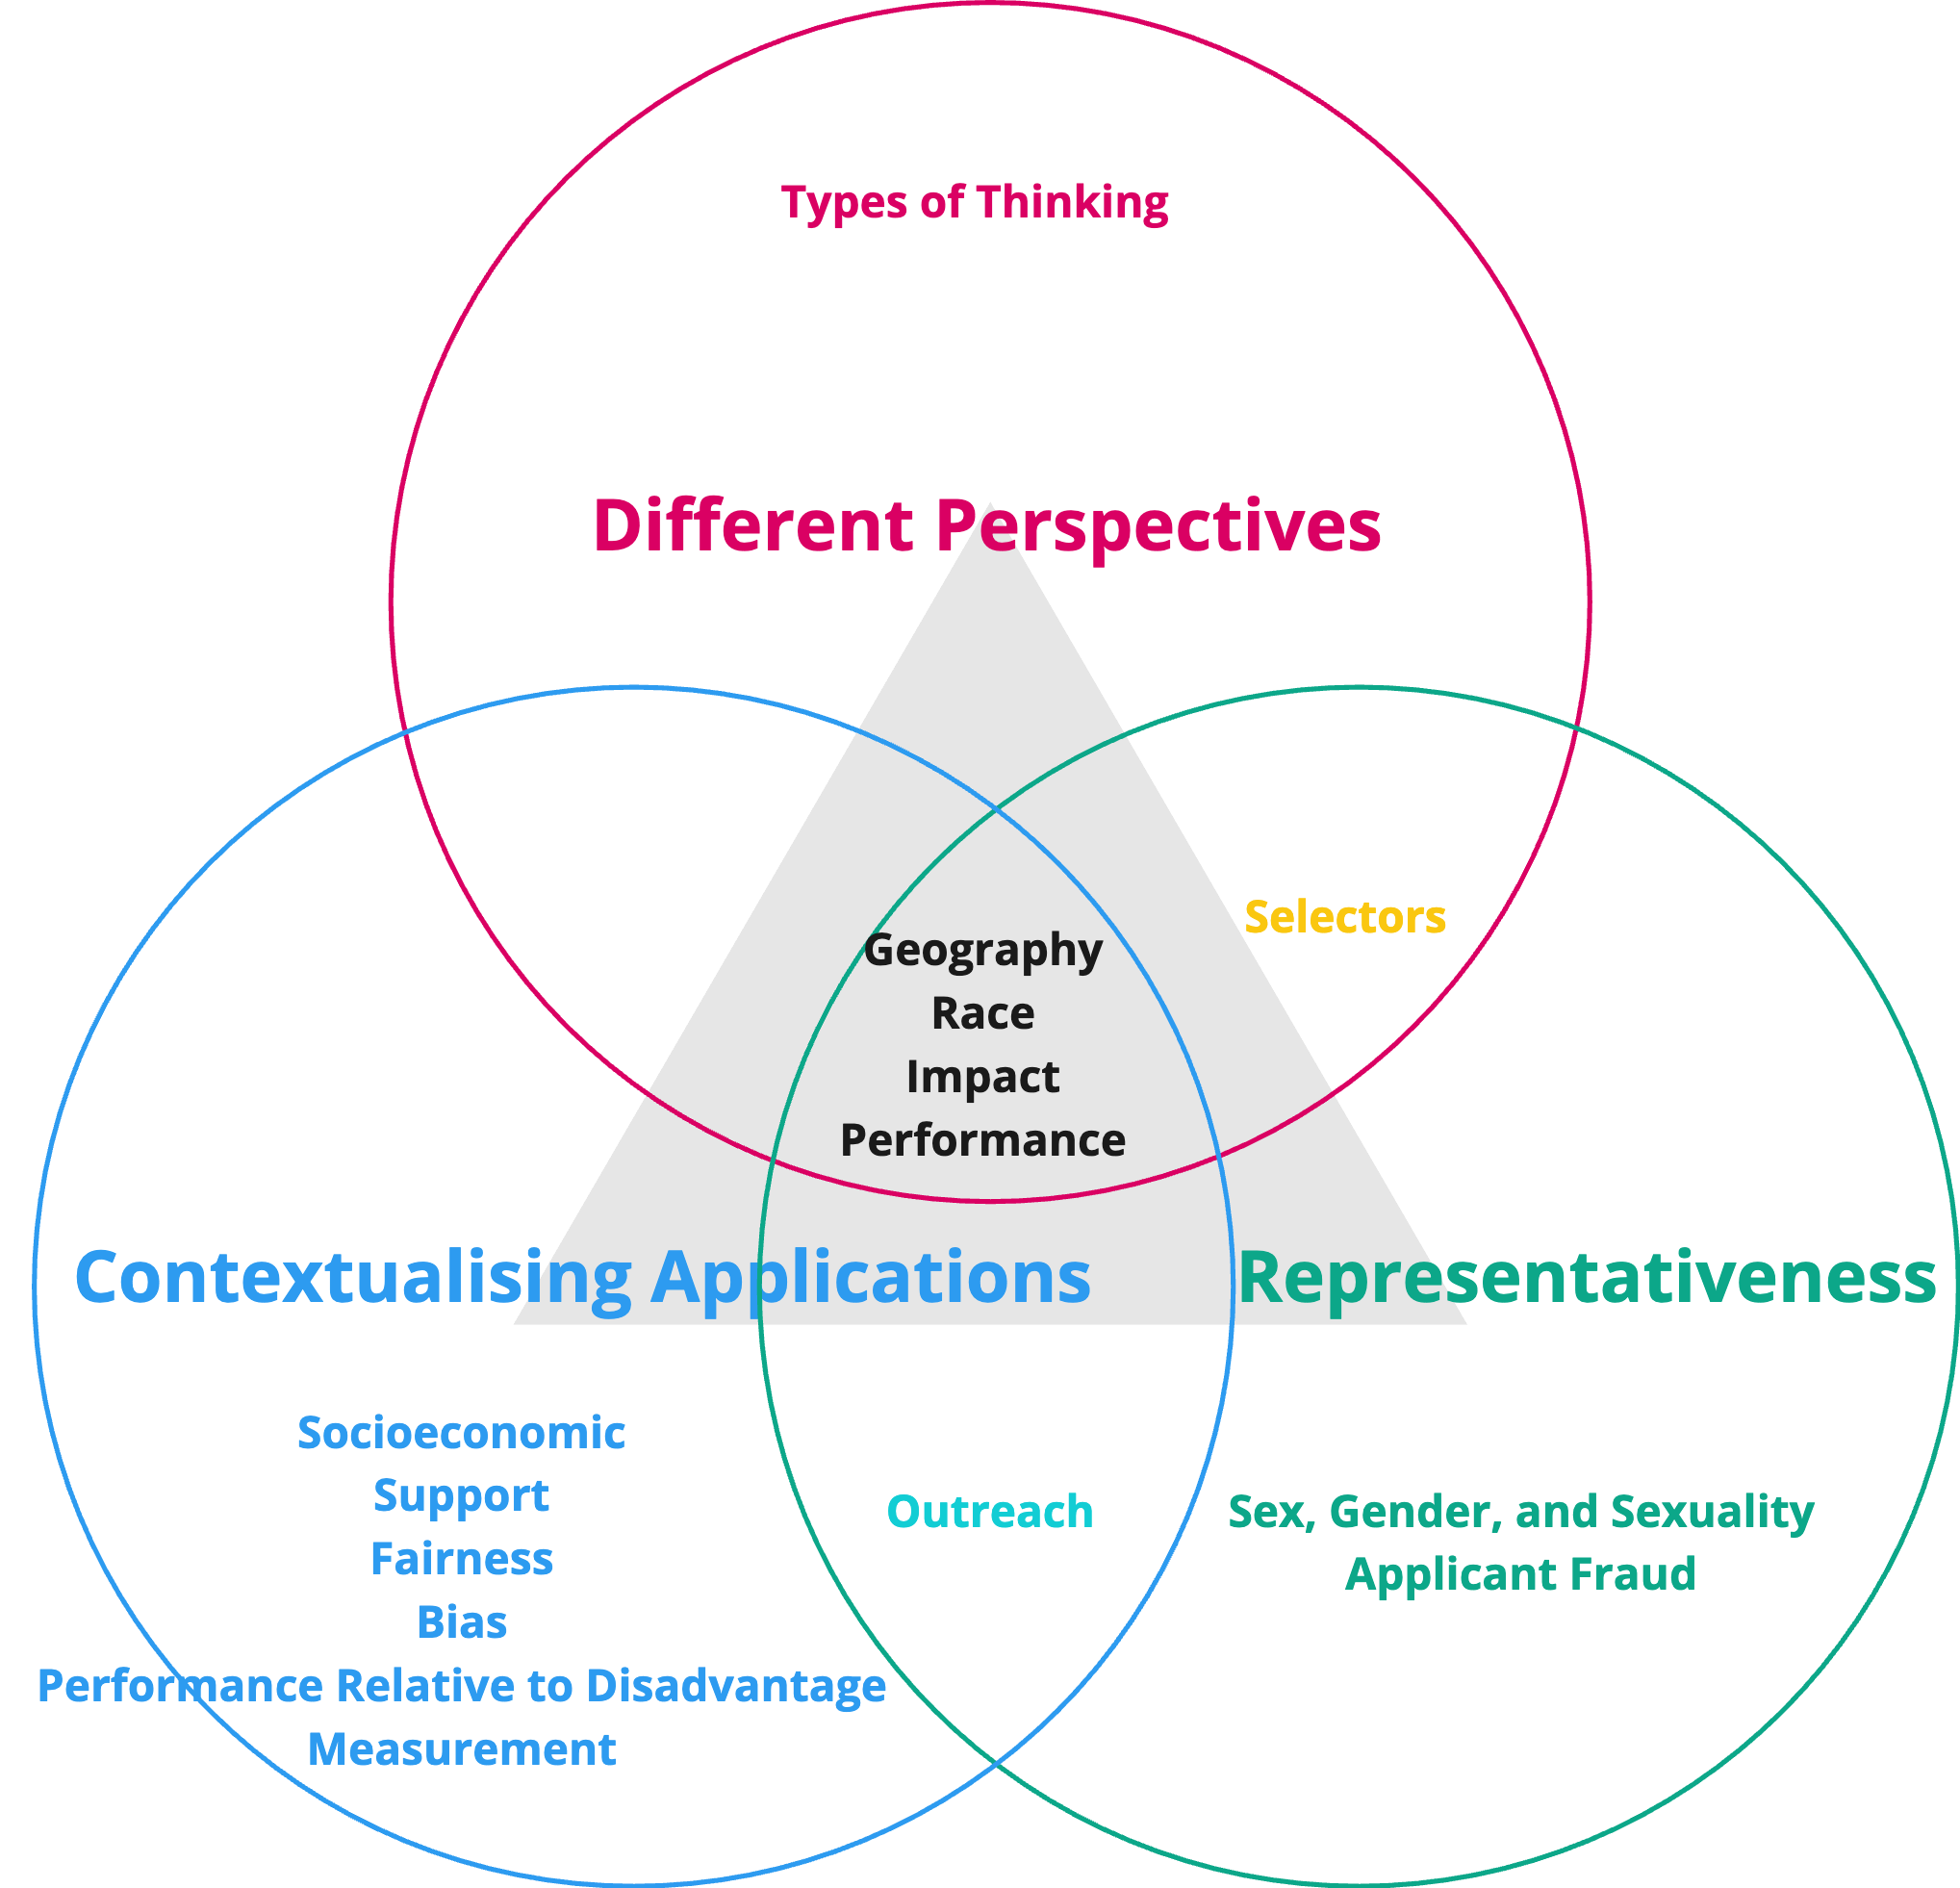
\includegraphics[width=\textwidth]{diversity/diversity_triangle.png}
    \caption{This figure depicts the \emph{Diversity Triangle}, three differing definitions of diversity selection practitioners expressed when discussing a diverse cohort. We also relate the Diversity Triangle to each other theme or subtheme participants mentioned.}
    \label{fig:div_triangle}
\end{figure}

\subsection{The Relationship Between the Diversity Triangle and Theories of Change}
\subsubsection{Representativeness}
Each of the definitions from the Diversity Triangle (Figure \ref{fig:div_triangle}) implies different program values and a different theory of change. The representativeness
definition relies on social theories by which diversity is intrinsically valuable. Several participants seemed to believe representativeness here was intrinsically valuable, which aligns with the \textcite{morris1984origins} account under which contemporary diversity norms emerged from loci of oppression affecting underrepresented groups. However, some participants also noted instrumental reasons to value representativeness that align closely with \textcite{peters2021hidden,page_difference_2007}'s argument that people from different backgrounds often posses unique and germane knowledge. One participant noted that a team can: ``Better serve a community if they represent [that community]'' (P9). Another theory from \textcite{Friedler_Scheidegger_Venkatasubramanian_2016} discusses measurement bias. Notably, if we assume that talent is equally distributed across some partition, then the most talented cohort should also be representative. However, \textcite{Friedler_Scheidegger_Venkatasubramanian_2016} note that we often observe in practice that performance is not equally distributed across these partitions. Depending on one's worldview, one might see this as due to inherent differences between those groups, or due to structural bias that causes differences in construct observability between them \cite{Friedler_Scheidegger_Venkatasubramanian_2016}. In the latter case, representativeness would be a proxy for fairness. Thus, representativeness is pro-social: society is better served when resources are distributed to a representative group of people.

\subsubsection{Different Perspectives}
The argument for placing different perspectives in the same room is often instrumental. While `diversity' on the whole is often spoken of as an intrinsically valuable broader benefit, the aim of placing different people in the same room is often only to benefit the people in that room. \textcite{page_diversity_2010} argues that `cognitively' diverse groups outperform homogeneous groups on some tasks; some participants similarly contend that it improves cohort-level task performance. Other participants echo \textcite{wylie2006introduction}'s argument that it allows participants to better learn from each other. In either case, the benefit is primarily organisational rather than social.

\subsubsection{Contextualising Applications}
The argument for contextualising applications is twofold. Most often, participants make a systemic critique here. That is, the world is incredibly unjust, and we want to distribute resources differently, but in a talent selection process we still have to operate in the unequal world. Thus, in order to correct for that injustice, we must give more resources to those who have less. This could be seen as a form of distributive justice or `affirmative action'. Participants argue (perhaps relatedly) that appropriately contextualising applications results in more successful applications from disadvantaged groups; this, in turn, allows these applicants to have a positive impact on their groups. Relatedly, either due to measurement bias, or due to differences in performance brought on by disparate access to resources, support, and opportunities, we may find that applicants from disadvantaged backgrounds appear worse on paper. In either case, correcting this through contextualisation may also build a more fair selection process and a more just world, yielding great benefit to society. On the organisational side, if contextualising applicants allows for the admission of more applicants from marginalised groups, they may be better suited to critiques of existing power structures, as they may have more informative experiences of oppression \cite{mills2015blackness}.

\subsection{A Cautionary Note On Designing for Diversity}
Decisions such as scholarship selection have long-reaching impacts for the applicants. A successful applicant to a scholarship program might thus attend a university they could not have otherwise attended. There, they will acquire skills and a network that will continue to impact them later in life. These impacts may even affect those close to them, as their better circumstances likely better the circumstances of their communities. Thus, it is simultaneously important to ensure that these opportunities are dispersed fairly and to ensure that all demographics are included among those selected.

This increases the importance of selecting a diverse group of people, and mandates that we do all we can to do so. Quantitative decision support tools may have a role to play in this, but two problems remain: data collection and data processing. Primarily, diversity data is often self-reported. Thus, we cannot use this naively to generate diverse cohorts, as doing so would yield a competitive advantage to candidates who lie on their declarations. Secondly, processing data automatically has its own drawbacks. AI systems are prone to bias \cite{Friedler_Scheidegger_Venkatasubramanian_2016}. And as these systems improve, it is unclear if they will help or harm our ability to select diverse cohorts.

However, it is important to note that both the problems of data collection and processing are not unique to this workflow. In fact, algorithmically-supported diversity considerations may correct for data collection and processing issues elsewhere. Bias is a major consideration in data collection \cite{Friedler_Scheidegger_Venkatasubramanian_2016}; heterogeneous biases in measurements of talent may be corrected by ensuring diversity across these metrics: ``Assessments are usually biased measures of what we actually care about, and that opportunity often correlates with positive error terms in assessments' measure of underlying skills.... [Diversity considerations] correct for the inadvertent affirmative action against underprivileged individuals implicit in using biased assessments'' (P1). Similarly, much like AI systems, human selectors are prone to their own heterogeneous biases; in some sense, `design for idiosyncrasies' reflects the notion that decision support systems must at times help recognise and mitigate these biases.

\section{Limitations and Future Work}
In Studies 1 and 2 we build tools with which participants report satisfaction, but increasing participant satisfaction does not necessarily improve decision-making. In particular, technology that makes difficult decisions less painful may be well-received, while technology that makes these decisions more salient may be less popular but more impactful \cite{Lipton,miller_explainable_2023}. Our themes speak to participant perceptions of diversity and our design recommendations speak to participant desiderata from support tools. We assume throughout that, in solving for these considerations, we can help organisations select better cohorts. However, we may find that these tools fail to improve decision-making with regards to diversity in practice. Future work should investigate this possibility through implementation of our prototypes in field settings.

\textcite{venn-wycherley_realities_2024} contend that HCI literature focused on educational contexts should consider both educator and student. Two distinctions distance our work from theirs: first, selection is distinct from pedagogy in that our decision subjects are not necessarily beneficiaries (while students are beneficiaries of their institution, applicants do not become beneficiaries unless they are selected); second, scholarships are distinct from educational institutions in that scholarship program benefits primarily focus on assisting beneficiaries in accessing educational institutions, while educational institutions primarily educate beneficiaries. Both distinctions create distance between selectors and applicants beyond that between teachers and students and pose challenges in engaging decision subjects. Nonetheless, future work should engage scholarship applicants to understand their definitions, stances, and considerations with respect to diversity. 

While not a limitation, we have intentionally set aside themes such as `outreach' and `selectors' that relate more to other aspects of selection processes than to the act of selection itself. We hope future work will consider these facets of selection programs, especially when designing tools to support thinking around diversity.

\section{Conclusion}
This research answers the crucial question: ``What is diversity?'', from the perspective of scholarship and talent investment selection practitioners. In doing so, we illuminate the multifaceted nature of diversity in scholarship selection and emphasise the critical need for tools that support considerations of diversity in decision-making. Our findings reveal that achieving true diversity involves navigating the complex interplay between three occasionally conflicting definitions: representativeness, diverse perspectives, and the contextualisation of applicants' backgrounds. By engaging in participatory design, we build six prototypes with our practitioners; this process reveals four design recommendations: design for a specific diversity, design for idiosyncrasy, design in stages, and design to balance quantitative and qualitative. This work demonstrates that, when thoughtfully designed, technology can empower selection processes to be more equitable, inclusive, and transparent. The broader implication is that such advancements have the potential to reshape how diversity is operationalised, ensuring that it is both a measurable outcome and a core value in shaping the future of talent identification. As we move forward, the integration of these tools into real-world practices will be pivotal in fostering truly diverse and representative groups in global scholarship programmes and beyond.
% \begin{savequote}[8cm]
% Alles Gescheite ist schon gedacht worden.\\
% Man muss nur versuchen, es noch einmal zu denken.

% All intelligent thoughts have already been thought;\\
% what is necessary is only to try to think them again.
%   \qauthor{--- Johann Wolfgang von Goethe \cite{von_goethe_wilhelm_1829}}
% \end{savequote}

\chapter{\label{ch:spf}A Possibility Frontier Approach to Diverse Talent Selection}

\minitoc

\section{Introduction}\label{sec:introduction}
The rise of diversity, equity, and inclusion initiatives suggests that various organizations (e.g. schools, firms, social impact programs, etc.) are genuinely interested in selecting for diverse talent. This is driven, at least in part, by recent declines in discrimination \cite{hsieh2019allocation}, increases in the perceived return to diversity \cite{deming2017growing, page2019diversity, noray2023systemic}, and increased social pressure for demographic representation \cite{minkin2023diversity}. In this paper, we hypothesize that the complexity of simultaneously optimizing for talent and diversity leads organizations (even well-intentioned ones) to select within their feasible talent-diversity frontier \cite{nemhauser1978analysis, huppenkothen2020entrofy}. This paper tests this hypothesis by demonstrating and incorporating this complexity into a simple model of cohort selection and testing the empirical predictions of the model using data from a high-profile scholarship and talent investment program. 

We begin by developing a simple model of cohort selection. Organizations receive $N$ applications and must select $n<N$ individuals to construct a cohort from the total set of potential cohorts, each of which is indexed by $c$. The organization seeks to maximize a preference function that is increasing in both a cohort's talent (e.g., the mean performance on an ability measure) and a cohort's diversity (e.g., an inverse distance to a set of target proportions of demographic groups). We then prove that this problem, though simple to state, is computationally complex. This is for two intuitive reasons. First, an individual's contribution to the diversity of the cohort depends on who else will be part of the cohort. Thus, to determine which cohort is the smallest distance from the predefined "ideal" diverse cohort, every possible cohort needs to be assessed. Second, when diversity preferences are for representation of at least two non-mutually exclusive identities (e.g. ethnic minorities and women), optimally selecting members of one group constrains your ability to do the same for the other group. Formally, we show that maximizing functions on subsets is in general non-polynomial. We then show that, when we restrict our attention to functions formalizing diversity as organizations measure it, the `Vertex Cover' problem, known to be $\mathbf{NP}$-hard, reduces to diversity maximization. This implies that calculating the maximal diversity conditional on cohort performance (what we refer to as the Selection Possibilities Frontier, or SPF) is also $\mathbf{NP}$-hard. Selecting on the SPF, then, is likely prohibitively costly for many organizations. 

To account for this complexity, we augment our model of cohort selection by forcing organizations to incur a computational marginal cost for each unit of increased cohort diversity. This represents the fact that, to find a more diverse cohort, one must engage in the laborious process of composing potential cohorts and comparing them. This is in sharp contrast to finding more talented cohorts, which is comparatively simple -- and, therefore, modeled as costless -- because each individual's contribution to cohort talent is unrelated to the remainder of the cohort. This simple model has two implications: (1) organizations will tend to select sub-optimal (i.e. non-first-best) cohorts and (2) organizations will improve on both performance and diversity if the gain access to a technology that reduces this computational marginal cost. 

We then develop an algorithm that can estimate the SPF in polynomial time. To do this we use optimization theory to show that a greedy algorithm can be used to approximate the maximal diversity as long as the function that maps cohorts to diversity scores is submodular, monotonic, and non-negative \cite{krause2014submodular, huppenkothen2020entrofy}. We then construct a formal algorithmic procedure that uses the greedy method to maximize a weighted sum of cohort diversity and cohort performance. Finally, we exploit the observation that the SPF is isomorphic to the diversity and talent levels of the set of cohorts that maximize the weighted sum for some value of the weights. Thus, we apply this procedure repeatedly using different weights to estimate the entire SPF. We also derive bounds for each estimated point on the SPF. 

Next, we turn to the empirical component of the paper where we test our model's predictions by applying the SPF estimate to selection data from a high-profile scholarship and talent investment program. The program aims to find talented high-schoolers from around the world and invest in them so they can realize their full career potential. The program provides winners with various benefits such as college scholarships, career support, and networking opportunities. When making decisions about which applicants to choose, the program weighs both cohort composition (i.e. diversity) and the cohort talent. For diversity, the program has clear preferences that the cohort be as close as possible to explicit proportions of various demographic groups defined along various dimensions such as gender, socioeconomic status, global region of origin, and country of origin. On the talent dimension, applicants are judged by experts primarily on the quality of concrete projects designed to showcase their potential (e.g. robots, mobile applications, engineering blueprints, etc.).

We start our empirical analysis by estimating SPFs for the first two consecutive application cycles and using them to test whether the program could have selected cohorts more efficiently. We find that, in cycle 1, the set of finalists could have been $18.5\%$ more diverse without any reduction in performance and $17.8\%$ higher-performing without any reduction in diversity. Similarly, in cycle 2, the finalists could have been $14.6\%$ more diverse without any reduction in performance and $24.1\%$ higher-performing without any reduction in diversity. Thus, both cohorts chosen were non-first-best as measured by the program's definitions of diversity and performance. We also show that in cycle 3, when the program was given access to the SPF, they significantly improved the efficiency of their selection process, choosing a cohort that was more diverse, higher performing, and essentially on the estimated SPF. This provides suggestive evidence that the SPF aided their decision-making and allowed them to better optimize in the face of a complex choice.

We conclude our empirical analysis by using our SPF estimation procedure to evaluate the efficacy of alternative screening and selection methods. To do this, we leverage two unique aspects of the program. First, the program collects both traditional merit-based measures -- including cognitive tests, written essays, and referring organizations -- as well as non-traditional measures -- including peer reviewed video essays, gamified skill tests, and application platform behaviors. Second, the program engaged in effectively no screening before receiving concrete projects from applicants, making it possible to estimate valid counterfactual diversity and performance of cohorts had they been screened in different ways. Leveraging these features, we find three key results. First, selecting only on the basis of cognitive ability or traditional metrics would have improved cohort performance relative to random selection, but would significantly restricted the program from reaching its diversity goals. By contrast, selecting only on peer reviews performs similarly on performance but improves diversity substantially. Second, all alternative selection methods we explore result in selecting cohorts well within the SPF and, therefore, leave substantial diversity and performance gains on the table. And third, the trade-off implied by the SPF between talent and diversity is steeper if traditional measures are used to measure talent than if applicant projects are used. 

This paper contributes to a growing economics literature studying the influence and potential of algorithms. Most research in this area has focused on measuring the effects of AI tools both at the economy-wide ("macro") level \cite{acemoglu2022automation,babina2024artificial,calvino2023portrait,zolas2021advanced,webb2019impact} and in more specific ("micro") contexts like bail decisions and radiology \cite{albright2023hidden,kleinberg2015prediction,stevenson2019algorithmic,angelova2023algorithmic,imai2023experimental,grimon2022impact,noy2023experimental,brynjolfsson2023generative,bundorf2019humans, mullainathan2019machine, ribers2020machine, agarwal2023combining}. This paper is more closely related to the small subset of this work that \emph{develops} AI tools to improve or assess human problem-solving in some respect.\footnote{Though small in economics, there is a larger literature in computer science that focuses on developing algorithmic tools to replace or improve humans' capacity to solve problems. Most closely related to this paper are machine systems that help organizations select in ways that are "unbiased" \cite{tambe2019artificial,raghavan2020mitigating} or account for "diversity" \cite{gillet2011diversity,huppenkothen2020entrofy}. Our paper differs from these because we account for trade-offs between diversity and other desiderata (e.g. talent, productivity, etc.).}  This includes work that develops methods to compare the efficacy of human vs. AI predictions \cite{kleinberg2018human,rambachan2024identifying} and several papers that develop algorithms specifically to improve the selection or assignment of personnel \cite{li2020hiring,bergman2021seven,kleinberg2018algorithmic,huppenkothen2020entrofy}. Our paper contributes to this literature by developing and applying algorithmic tools to the increasingly relevant diverse talent selection problem. 

Our paper is closely related to \textcite{kleinberg2018algorithmic}, which introduces an algorithm that colleges can use to calculate the most meritorious cohort at any threshold of representation for a single underrepresented group. Their algorithm is straightforward: define a minority group (e.g. black applicants) and the corresponding majority group (e.g. white applicants), rank applicants within each group by measure of merit (e.g. test scores, predicted college performance, etc.), set a threshold for the proportion of those selected who should be part of the minority group, select minority group members from the highest ranking down until the threshold is met, and finally, select the majority group members from the highest ranking down until all slots are filled. Though effective, this procedure only works when the organization aims to represent mutually exclusive minority groups. If diversity preferences are instead for representation of multiple non-mutually exclusive groups (e.g., female applicants and black applicants), this strategy no longer works. This paper relaxes this assumption and outlines the conditions under which the diversity-performance frontier can be estimated regardless of the number or type of identity characteristics organizations seek to represent.

This paper is also related to the growing economics literature on the impact of new screening technologies on the productivity and diversity of the personnel that organizations select. An early paper on this topic is \textcite{autor2008does}, which shows that adding personality tests to the job applicant screening process in a national retail firm increased the productivity of selected workers without reducing minority representation among hires. More recently, \textcite{li2020hiring} demonstrate that, within a Fortune 500 tech company, diversity and productivity of hires can be improved by using exploration-based applicant screening algorithms that recommend applicants with rare sets of characteristics at higher rates in order to improve noisy predictions and, therefore, learn how to find promising applicants from atypical backgrounds. Similarly, \textcite{bergman2021seven} show that, across seven colleges, using a prediction algorithm instead of a test to decide whether to place students into remedial classes improves student performance and increases minority representation in college-level (non-remedial) courses. Our paper adds to this literature in two ways. First, rather than focusing on comparing a new screening method to the status quo, this paper develops a procedure for estimating the diversity-performance frontier itself. Second, leveraging the novel design of the scholarship's application process in combination with our estimate of the SPF, we provide new evidence on the efficacy of screening on traditional "merit" measures. 

This paper is also related to work across fields defining fairness and equity in talent selection. Much of this work builds on the \emph{similar treatment principle} whereby individuals who perform similarly on some dimension(s) are treated equally in selection \cite{dwork_fairness_2012}.\footnote{Though not generally mentioned in this literature, the similar treatment principle is the normative basis on which differential treatment of demographic groups in audit studies is deemed wrong.} This approach has been criticized, however, on the grounds that in circumstances when performance and demographic factors are correlated, employing this principle could substantially reduce the diversity of the chosen cohort, which may not accord with a decision-makers fairness preferences \cite{fleisher2021s}. Furthermore, when measurements of performance are biased in favor of certain demographic groups, similar treatment on the basis of these measurements leads to applicants with the same underlying ability being treated differently \cite{fleisher2021s}. An alternative perspective is to assume fairness and equity are captured by diversity, and instead to measure diversity directly. Three measures are commonly considered: (1) the majority-minority approach, (2) the generalized variance approach, and (3) the entropy statistic (see \textcite{budescu2012measure} for a summary). Following \textcite{huppenkothen2020entrofy}, we measure diversity using an entropy-based approach. We do this for two reasons. First, as \textcite{huppenkothen2020entrofy} demonstrate, versions of an entropic scoring function have mathematical properties (i.e. submodularity and monotonicity) that allow us to both easily estimate the SPF and to bound the error of our estimates. Second, preferences for diversity often take the form of ``closeness to a proportional target for each relevant identity characteristic'', which can be represented easily using entropic functions. Thus, our work adds to the applications of entropy-based methods for measuring diversity.

The rest of the paper is summarized as follows. Section \ref{sec:model} introduces a simple model of cohort selection with complexity costs and micro-founds the complexity costs by demonstrating the complexity of diversity maximization. Section \ref{sec:spf_alg} we defines the selection possibility frontier, presents an algorithm that generates an estimate of the SPF, and formally derives bounds on these estimates. In Section \ref{sec:case} we apply the SPF procedure to characterize the selection inefficiencies of a talent selection program, show efficiency improvements after using the SPF, and asses the efficacy of alternative screening algorithms. In Section \ref{sec:conclusion}, we discuss our findings and reach a conclusion. 


\section{Building A Model of Diverse Talent Selection With Complexity}\label{sec:model}

In this section we develop a model of diverse talent selection with complexity costs. We start by outlining a solution to a simple version of this problem with no complexity. This allows us to introduce the problem, build intuition, and formally define a key object referred to throughout the paper called the Selection Possibilities Frontier (SPF). We then prove that, under standard definitions of diversity, this problem is computationally complex (i.e., it cannot be solved in polynomial time), which makes finding the optimal solution impractical. We conclude the section by embedding this complexity into the model by representing it as a computational marginal cost. This augmented version of the model yields two testable predictions: (1) organizations will select sub-optimal (i.e. non-first-best) cohorts and (2) organizations can improve on both performance and diversity if the computational cost is reduced. 

\subsection{Diverse Talent Selection Without Complexity}\label{subsec:simple_model}

We start by considering a simple version of the organization's optimization problem without complexity. Organizations receive $N$ applications and must select $n<N$ individuals to form a cohort $c$ from the set of all potential cohorts $C$. The organization prefers both that the selected cohort is higher performing on some measure of talent\footnote{Throughout the paper, we use ``talent" and ``performance" interchangeably, but both refer to performance on some sort of ability assessment.} and more diverse. For now, a cohort's diversity can be thought of as the inverse of a multidimensional measure of distance between the set of proportions of the cohort who belong to key demographic groups and a set of target proportions the organization has for each group (we discuss definitions of diversity in more detail in Section \ref{subsec:dts_nphard}). If we let the performance and diversity of a given cohort $c$ be given by the functions $P(c)$ and $D(c)$, respectively, then the above description is equivalent to letting the organization's preference function $F\Big(D(c),P(c)\Big)$ exhibit $F_D>0$, $F_P>0$, and $F_{DP}\geq0$, where subscripts indicate partial derivatives with respect to the variable in the subscript. 

Conceptually, this would represent a scenario where an organization can observe $D$ and $P$ for every possible cohort and simply select the one that maximizes $F(D,P)$. If we assume the organization behaves rationally, we know the organization will not choose dominated cohorts. Formally, $c^*$ can be the optimal cohort if and only if there exists no $c'$ such that $D(c')>D(c^*)$ and $P(c')\geq P(c^*)$ and there exists no $c'$ such that $D(c')\geq D(c^*)$ and $P(c')> P(c^*)$. We know that the optimal cohort must be in the set of non-dominated cohorts which we define as the Selection Possibilities Frontier (SPF). If we assume, for expositional purposes, that the SPF is continuous, we can represent it as the following function:

\begin{equation}
G(p) := \max\Big[D(c)|P(c) \geq p\Big]
\end{equation}

\noindent In words, $G(p)$ merely gives the highest possible diversity for every cohort performance level. The diverse talent selection problem, then, can be represented as choosing a cohort to maximize $F$ subject to a constraint that the choice be on the SPF. Formally, 

\begin{equation}
\max_{d,p} F\Big(d,p\Big) \text{ \bf{ s.t. } } d = G(p), \nonumber 
\end{equation}

\noindent which is equivalent to

\begin{equation}
\max_{p} F\Big(G(p) ,p\Big). \label{eq:selection_simple}
\end{equation}

The solution to this simple version of the model is depicted in Figure \ref{fig:model_spf}. The solid blue curve represents the SPF, the dotted blue curve represents the organization's indifference curve corresponding to the highest achievable utility, and the blue dot represents the diversity and performance of the optimal choice (i.e. the first-best solution). 

\subsection{Why Diverse Talent Selection is Complex}\label{subsec:dts_nphard}

So far we have assumed that the organization could costlessly select the cohort on the SPF that maximizes utility. But, what if identifying the first-best cohort is prohibitively costly? In this section we show that, under standard definitions of diversity, the problem is computationally complex (i.e., there is no known algorithm that can solve this problem in polynomial time). In other words, this problem is prohibitively costly to solve in practice. We use this finding as the micro-foundation for a computational marginal cost term which we add to the model, which we use to derive testable predictions. We break our discussion of this problem's complexity into two parts. In Section \ref{subsubsec:int_nphard} we present the intuitive explanation and in Section \ref{subsubsec:proof_nphard} we prove $\mathbf{NP}$-hardness. 

\subsubsection{Diversity Causes Complexity: An Intuitive Explanation}\label{subsubsec:int_nphard}

One way to see why the diverse talent selection problem is complex is to consider how it differs from a simpler special case where an organization only wants sufficient representation of one group. For example, consider a college that aims to accept some target fraction of Black applicants from a pool of Black and white applicants. And, assume the school wants to select as talented a class as possible, where talent is proxied for by test scores, grades, or some combination of the two. In this special case, as shown in \textcite{kleinberg2018algorithmic}, there exists a computationally easy algorithm to calculate the SPF shown below.\footnote{Technically, the algorithm presented by \textcite{kleinberg2018algorithmic} only optimizes for the \emph{most diverse} point on the SPF. Thus, we have added the \textbf{Repeat} step (cycling through the algorithm with different representation thresholds) to enable their algorithm to trace out the SPF.}

\begin{algorithm}
    \caption{A Procedure For Calculating the SPF Based on \textcite{kleinberg2018algorithmic}}\label{alg:kleinberg}
    \begin{algorithmic}
        \State \textbf{Define} a minority group (Black) and mutually exclusive majority group (white), 
        \State \textbf{Rank} applicants within their group by test score,
        \State \textbf{Define} a target proportion of Black admits,
        \State \textbf{Select} Black applicants from the highest ranking down until the target is reached,
        \State \textbf{Select} the white applicants from the highest ranking down for remaining slots,
        \State \textbf{Repeat} steps 1-5 for different thresholds of representation to trace out the SPF.
    \end{algorithmic}
\end{algorithm}

What allows this algorithm work is the \emph{mutual exclusivity} of the minority and majority group. This allows one to transform the diverse talent selection problem into two separate talent maximization problems where the organization simply selects the most talented members of each group. This can be extended to any case where target proportions are defined at the level of mutually exclusive group level, even when multiple different demographic dimensions are considered. To be concrete, if the school actually cares about race and gender and, thus, has target proportions for black male, black female, white male, and white female applicants, then the problem can be broken into four separate talent maximization problems where the most talented members of each group are selected until the target proportions are met for each group. 

But what happens if an organization has preferences for representation of \emph{non-mutually exclusive groups}? To continue the running example, this would be analogous to a college that has target proportions for black applicants and female applicants, but not for each race by gender combination. This seemingly small change prevents an organization from transforming the problem into simpler group-specific talent maximization sub-problems. To see this, consider applying the \textcite{kleinberg2018algorithmic} algorithm to each group sequentially; this would mean selecting the best black applicants until reaching the target proportion, then doing the same for female applicants. If the most talented black applicants were male or if there are few talented white females in the pool, having allocated the black slots in this way forces the college to select less talented females than optimal (or, it may inhibit reaching the target proportion for females at all). In short, when diversity preferences are over non-mutually exclusive groups, we cannot cleanly break the problem into simple talent maximization subproblems for disjoint minority groups, so it is not clear how we might extend the \textcite{kleinberg2018algorithmic} algorithm to a general version of the diverse talent selection problem. 

The general diverse talent selection problem, which is the focus of this paper, allows organizations to have preferences for representation of an arbitrary number of overlapping (or disjoint) demographic groups. This aligns more closely with the diversity preferences of real world organizations like colleges, firms, and social impact programs many of which aim to select personnel from various ethnicities, genders, classes, geographies, ideologies, and specialties. Organizations generally state their preferences using statements of the following form: ``the organization desires at least $x\%$ of group $g$'' or ``the organization desires at least one person from $m$ groups". These types of diversity preferences are what is formalized in the function $D(c)$, which will ultimately be defined as an aggregation of a version of the cohort's inverse distance to each diversity goal. We will show that under this conception of $D(c)$, maximizing $F\Big(D(c),P(c)\Big)$ belongs to a class of computationally complex problems. A formal proof of this is included in Subsection \ref{subsubsec:proof_nphard}.

One way to see why this problem is complex is to consider the relationship between cohort diversity and an applicant's demographic characteristics. Each individual applicant's contribution to diversity depends not only on her own demographics, but the demographic make-up of the rest of the cohort.\footnote{Note that in the special case where preferences are for representation of mutually exclusive groups, individual contributions to diversity can be known before constructing the entire cohort because the proportion of the cohort that will be a member of each group is determined and held constant at the start of the problem. This means that each individual selected until the target proportion from their group gets the organization exactly one person closer to the target.} This means that the cohort's diversity can't be known until an entire cohort is constructed. This implies that, in general, every possible cohort needs to be observed before determining which one has the highest level of diversity. This creates a numerical challenge when faced with any sufficiently large application pool. For example, in the context of the scholarship program we analyze in this paper, they are choosing roughly 500 finalists from over 2000 applications. Finding the most diverse cohort, therefore, would entail constructing $\frac{2000!}{500!(2000-500)!} \approx 5.648\times10^{486}$. This problem remains a real challenge when considering other contexts like university admissions, where major US universities receive tens of thousands of applications a year, or large firms, where many Fortune 500 companies hire thousands of employees per year.  

\subsubsection{The Complexity of Preference Functions}\label{subsubsec:proof_nphard}

Without restrictions on the types of functions that organisations may select for $D$, $P$ the most we can say of $F$ is that its domain is $C$ and its range is $\mathcal{R}$. We prove here that optimising this class of functions is computationally complex.

First, we introduce notions of computational complexity from computer science. The field of computer science considers a problem ``computationally simple'' if that problem is solvable in polynomial time (i.e., if there exists a program guaranteed to output the correct answer in a number of steps upper bounded by some polynomial function of the input). This class of problems is referred to as $\mathbf{P}$. A problem is ``computationally complex'' if it is not computationally simple, i.e., if it cannot be solved in polynomial-time. In this section, we prove outright that optimizing an arbitrary function on subsets with a fixed cardinality constraint significantly smaller than the universe size is computationally complex. I.e., Theorem \ref{thm:general-nphard} holds.

\begin{theorem}\label{thm:general-nphard}
    This is a thm.
    % Let $U$ be a `universe' set of size at least $N \geq 2*n$ and $S = \{s: \mathcal{P} (\mathbb{U}) \rightarrow \mathcal{R}\}$ be the set of functions with domain  $\mathcal{P} (\mathbb{U})$ and range $\mathcal{R}$. Then $Opt_{gen}(s_i, n) := argmax_{c \in U \and |c| = n}(s_i(c))$ is not $\mathbf{P}$ in $n$.
\end{theorem}

\begin{proof}
Suppose for a contradiction that $\forall s_i \in S . Opt_{gen}(s_i, n)$ can be solved by some algorithm $Alg_{gen}(s_i, n)$ which makes fewer than $n^m$ calls of $s_i$ for some fixed $m$. Let $n$ be sufficiently large that that $\choose{2n}{n} > n^m$. Then let $s_j$ be defined as follows:

\begin{equation}
s_j(c) = 
    \begin{cases} 
        Alg_{gen}(s_i, n) \text{ calls } s_i(c) & s_i(c) \\
        Alg_{gen}(s_i, n) = c & s_i(c)          \\
        \text{otherwise} & Opt_{gen}(s_i, n) + 1 
    \end{cases}
\end{equation}

\noindent As $s_i$ and $s_j$ are identical where $Alg_{gen}(s_i, n)$ calls $s_i$, they must also be identical where $Alg_{gen}(s_j, n)$ calls $s_i$. Thus, $Alg_{gen}(s_j, n) = Alg_{gen}(s_i, n)$.

By assumption, $Alg_{gen}(s_j, n) = Opt_{gen}(s_i, n)$, but as $\choose{2n}{n} > n^m$, $\exists c \subset U . s_j(c) = Opt_{gen}(s_i, n) + 1$. Thus, $Alg_{gen}$ is does not satisfy Theorem \ref{thm:general-nphard}, a contradiction!
\end{proof}

\subsubsection{Defining of Diversity and Talent}\label{subsubsec:div_talent_def}
While interesting, the results that the above class of problems is not $\mathbf{P}$ stops short of informing diversity optimisation in practice. Indeed, though the general class of functions is computationally complex, it could be that specific sub-problems are computationally fast. (In fact, the sub-problem identified by \textcite{kleinberg2018algorithmic} is computationally fast. We discuss further in Section \ref{subsubsec:int_nphard}.)

However, we contend that the mathematical structure implied by common notions of diversity causes the diverse selection problem to be complex. To prove this, we need to settle on more precise diversity functions that correspond to these common notions. In particular, we will formalize \emph{proportional diversity} and \emph{count diversity}. 

\emph{Proportional diversity} is what organizations seek when they make statements like ``we desire at least $x$ percent of group $g$". But, since organizations aim to select cohorts of a specific size, we can reframe this goal as ``we desire at least $x*n$ individuals from group $g$", where $n$ is the total number of applicants in the cohort.\footnote{This reframing will turn out to be helpful in Section \ref{sec:spf_alg} when we develop our SPF estimation strategy} If we let $\chi_g(c)$ be the proportion of $c$ in group $g$ and $\sigma_g(c)$ bne the total number of applicants in $c$ who are in group $g$ This can be formalized into the proportional diversity function

\begin{equation}
    \begin{split}
        \delta_{g}^{prop}(c,x) &:= n*\min(\chi_g(c), x) \\
        & := \frac{n* \min(\sigma_g(c), x*n)}{n} \\ 
        & := \min(\sigma_g(c), x*n). \label{eq:prop_div_function}
    \end{split}
\end{equation}

If, for example, an organization selecting 100 applicants would like their organization to be least $40\%$ female the proportional diversity function associated with this goal is $\delta_{female}^p(c, 40) := \min(\vec{\mathbf{f}}*\vec{\mathbf{c}}, 40)$ where $\vec{\mathbf{f}}$ is a Boolean vector indicating which applicants are female and $\vec{\mathbf{c}}$ is a Boolean vector that indicating who is in cohort $c$. This can be thought of as an inverse distance along the dimension of group representation between cohort $c$ and an ideal cohort $c^*$ where $\sigma_g(c^*) = x*n$.

The second common type of diversity is what we call \emph{Count diversity}. This is what organizations are after when they make statements like ``we desire at least one person from $m$ groups". To formalize this notion, let $\mathbb{I}(\cdot)$ be an indicator function that is equal to 1 if the condition within is true. We can now represent a count diversity preference as

\begin{equation} 
    \begin{split}
        \delta_G^{count}(c,m) &:= \min\big(\sum_{g \in G}\mathbb{I}(\sigma_g(c)\geq 1), m\big), \label{eq:count_div_function}
    \end{split}
\end{equation}

\noindent where $G$ is the set of relevant groups the organization wants represented by at least a single individual. This type of function is ideal for representing geographic representation goals where educational institutions, like colleges or scholarships, often have goals like ``we want a student from every state" or ``we want as many countries as possible represented". 

Ultimately, organizations care about all of their diversity goals, not just one. Thus, the diversity functions that are relevant for an organization must be aggregated if we want to formalize an organization's overall preference for diversity. We define this aggregation as an organization's diversity score $D(c)$, which generally has the following form: 

\begin{equation}
A\big(\delta_{g_1}^{prop}(c,x_1),...,\delta_{g_K}^{prop}(c,x_K),\delta_{G_1}^{count}(c, m_1),...,\delta_{G_J}^{count}(c, m_J)\big), \nonumber
\end{equation}

\noindent where $A(\cdot)$ is an aggregator function. It is essential that $D(c)$ increases as a cohort gets ``closer" to one of the underlying diversity goals because this is sufficient to identify cases when one cohort dominates another, even if the formalization misses something subtle or difficult to articulate about the organization's diversity preferences. A flexible but simple aggregator function is a weighted sum, where organizations can place different emphasis on each of the goals. So, for the remainder of this paper, we use diversity scores of the following form: 

\begin{equation}\label{eq:d_equation}
D(c,\vec{\mathbf{w}},\vec{\mathbf{x}},\vec{\mathbf{m}}, \vec{\mathbf{g}}, \vec{\mathbf{G}}) := \sum_{k\in K}w_k\delta_{g_k}^{prop}(c,x_k) + \sum_{j \in J}w_j\delta_{G_j}^{count}(c, m_j),
\end{equation}

\noindent where $\vec{\mathbf{w}},\vec{\mathbf{x}}, \vec{\mathbf{m}}, \vec{\mathbf{g}}, \vec{\mathbf{G}}$ are vectors of the organization's weights, proportional targets, count targets, groups of interest to proportional diversity functions, and sets of groups of interest to count diversity functions, respectively.\footnote{Another attractive option is a CES aggregator because it allows for specifying degree of substitutability between diversity goals, but this comes at the cost that many organizations don't really know this (introducing similar problems as requiring goals at the mutually exclusive group level). Nonetheless, the authors are currently working on establishing whether the estimation procedure presented in Section \ref{sec:spf_alg} is viable for a CES aggregator.} In general, we suppress the vector notation opting to refer to the diversity score as $D(c)$ where this doesn't lead to confusion.

Our definition of talent is comparatively simple. In general, organizations define talent as some sort of performance metric. Common examples include test scores and grades for educational organizations or technical interviews for tech hiring. More sophisticated (though uncommon) measures might be the predicted success of an individual based on a set of performance metrics. In this paper we assume there is a real-valued talent metric $\rho_i$ evaluated at an individual-level. A cohort's \emph{talent}, then is defined as the sum of the talent level of the individual members, which is given by

\begin{equation}
P(c) := \sum_{i \in I_c}\rho_i,
\end{equation}

\noindent where $I_c$ is the set of all individuals $i$ in cohort $c$. Unlike with diversity, $P(c)$ is straightforward because each individual's contribution is $\rho_i$ regardless of whoever else is in the cohort. Ultimately, this will justify adding a computational cost to our model that is asymmetric, applying to diversity and not to talent.

We represent an organisation's preference function $F$ as a weighted sum of performance and diversity functions. That is:

\begin{equation}\label{eq:f_spec}
F(D, P, c, \iota) := \iota*D(c)+(1-\iota)*P(c)
\end{equation}

\subsubsection{The Complexity of Our Preference Functions $F$}

Much like the class of $\mathbf{P}$ problems, there is a second class of problems, $\mathbf{NP}$ that are \textit{verifiable} in polynomial time. It is often assumed in Computer Science (though unproved) that $\mathbf{P} \neq \mathbf{NP}$, i.e., that there exist problems in $\mathbf{NP}$ that are not in $\mathbf{P}$; we make this assumption here \cite{COPPERSMITH198527}. Yet a third class, the class of ``$\mathbf{NP}$-hard'' problems, are the problems whose solutions can be used to emulate (with a polynomial-time emulator) solutions to all $\mathbf{NP}$ problems. If $\mathbf{P} \neq \mathbf{NP}$, then all $\mathbf{NP}$-hard problems are not polynomially solvable.

We also bring in the notion of `reduction'. A reduction is simple: $A \leq B$ (i.e., $A$ reduces to $B$) if and only if there exists a polynomial time algorithm that makes some polynomially bounded number of calls to $B$ and thus returns an answer to $A$. In other words, we say that $A$ is $\mathbf{NP}$-hard if and only if $\forall B \in \mathbf{NP} A \leq B$. It is clear to see, then, that if $B$ is $\mathbf{NP}$-hard and $A \leq B$, then $A$ is also $\mathbf{NP}$-hard.

We now prove that, when $S$ is restricted to only equations of the form $F$ from Equation \ref{eq:f_spec}, the problem of finding the optimal subset of size $k$ for any $s_i \in S$ is still computationally complex. This time, we rely on the assumption that $\mathbf{NP}$-hard problems are computationally complex. That is, Theorem \ref{thm:specific-nphard} holds. 

\begin{theorem}\label{thm:specific-nphard}
    This is another theorem
    % Let $U$ be a `universe' set of size at least $N \geq 2*n$ and $S = \{s: \mathcal{P} (\mathbb{U}) \rightarrow \mathcal{R}\}$ be the set of functions of type $F$ described in Equation \ref{eq:f_spec}. Then $Opt_{spec}(s_i, n) := argmax_{c \in U \and |c| = n}(s_i(c))$ is $\mathbf{NP}$-hard in $n$.
\end{theorem}

In order to do this, and to justify the significance of this result, we bring in the computational complexity of the $VertexCover$ problem, which has been proven to be $\mathbf{NP}$-hard \cite{COPPERSMITH198527}. $VertexCover$ can be seen in Theorem \ref{thm:vertexcover}.

\begin{theorem}\label{thm:vertexcover}
    This is another theorem
    % Let $G = (V, E)$ be a graph. Let $VC(G, \kappa) := Cov | Cov \subseteq V \and |Cov| = \kappa \and \forall e \in E . \exists v \in Cov . v \in e$ be a function of $G$ that returns a set $Cov$ such that every edge in $G$ is incident on at least one vertex in $Cov$. Then $VC$ in $\mathbf{NP}$-hard in the number of vertices.
\end{theorem}

We now prove Theorem \ref{thm:specific-nphard} by reduction to Theorem \ref{thm:vertexcover}.

% \begin{proof}
% Suppose for a contradiction that Theorem \ref{thm:specific-nphard} admits some polynomial-time solution $Alg_{spec}$. I.e., $Alg_{spec}(s_i, k )= argmax_{c \in U \and |c| = n}(s_i(c))$.

% \begin{algorithm}
%     \caption{An Algorithm for $VC(G = (V,E), \kappa)$}\label{alg:vc_spec}
%     \begin{algorithmic}
%         \State \textbf{Consider} $U := E$
%         \State \textbf{Define} $\vec{\mathbf{g}} := \{g_i = v_i \in e . e \in E | i \in |V|\}$ such that each $g_i$ has length $E$ and corresponds to whether an edge is incident on vertex $v_i$.
%         \State \textbf{Return} $Opt_{spec}(1*D(c, \vec{\mathbf{1}}, \vec{\mathbf{0}}, \vec{\mathbf{0}}, \vec{\mathbf{g}}, \vec{\mathbf{0}})+ 0*P(c)) \geq k$
%     \end{algorithmic}
% \end{algorithm}

% Then consider the algorithm $Alg_{VC}$ that is defined in Algorithm \ref{alg:vc_spec}. But this algorithm solves $VertexCover$ in polynomial time relative to $Opt_{spec}$, and thus is a polynomial time solution to $VertexCover$. Assuming $\mathbf{P} \neq \mathbf{NP}$, contradiction!
% \end{proof}

\subsection{Embedding Complexity into the Model}\label{subsec:dts_w_complexity}

To incorporate complexity, consider a variation of the simple cohort selection problem (see Section \ref{subsec:simple_model}) where the organization can search for increasingly diverse cohorts at a cost. Let the amount of search effort be $e\in[0,1]$ and define the cost of search effort be $\alpha p(e)$ where the cost is convex (i.e. $p_e>0$ and $p_{ee}>0$) and $\alpha$ is a constant that is inversely related to the quality of search technology available. Furthermore, we let the amount of search deterministically increase the maximum achievable diversity at each talent level, which is now given by $D^{SPF}*e$. The optimization problem can then be rewritten as:

\begin{align}
&\max_{d,p,e} F\Big(d,p\Big) - \alpha p(e) \text{ \bf{ s.t. } } d = G(p)*e, \nonumber \\ 
& \implies \max_{p,e} F\Big(\underbrace{G(p)*e}_{\text{Info Cost}} ,p\Big) - \underbrace{\alpha p(e)}_{\text{Direct Cost}}. \label{eq:objective}
\end{align}

It is clear from the form of the organization's new objective function in Equation \ref{eq:objective} that complexity of maximizing diversity imposes two kinds of costs: an information cost that represents the fact that the organization will generally not know which cohort is on the SPF and a direct search cost. Also, when search costs are set to zero (i.e. $\alpha=0$), the problem collapses into the original problem because searching is costless and, therefore, maximized at $e=1$. But, when $\alpha>0$, the optimal cohort will now be inside of the SPF. This is because, for all $c'$ such that  $D(c')=G(p(c')=p')*e$ there exists $c^f$ on the SPF such that $D(c^f)=G(p(c^f)=p')$. Thus, as long as the optimal effort is below 1, any solution to this problem will result in selecting a cohort that is within the SPF and, therefore, non-first-best. This leads to the first prediction from this model: \\

\noindent \textbf{Prediction 1}: \emph{When complexity-induced search costs are sufficiently high, organizations will select cohorts within the SPF.} \\

The solution to the selection problem with complexity is depicted in Figure \ref{fig:model_complex}. As before, the solid blue curve represents the SPF, the dotted blue curve represents the organization's indifference curve corresponding to the highest achievable utility without search costs, and the blue dot represents the diversity and performance of the first-best solution. But, added to the figure is now a solid red curve which represents the accessible frontier with optimal search, a dotted red curve that represents the highest achievable utility with search costs, and a red dot that represents the diversity and performance of the optimal cohort with search costs (i.e. the second-best solution). 

Additionally, the extent of the inefficiency will tend to reduce as complexity costs reduce. We can see this by examining the comparative statics of the model. To simplify our derivation of the relevant comparative static, we refer to the organization's objective function as $O(p,e)\equiv F\Big(G(p)*e ,p\Big) - \alpha p(e)$. Furthermore, we use subscripts on functions refer to partial derivatives and we drop the arguments of functions where this causes no confusion. The (necessary) first order conditions from this model are, therefore, the following:

\begin{align}
O_p & \equiv F_{d}(G(p)e,p)G_p(p)e + F_p(G(p)e,p) = 0 \nonumber \\
O_e & \equiv F_{d}(G(p)e,p)G(p) - \alpha p_e(e) = 0. \nonumber
\end{align}

To ensure this is a maximum, we also need to assume that the (sufficient) second order conditions hold. They are the following:

\begin{align}
O_{pp} \equiv &\;  e^2G_p^2F_{dd} + 2eG_pF_{dp} + eG_{pp}F_d + F_{pp} < 0, \nonumber \\
O_{ee}  \equiv &\;  G^2F_{dd} - \alpha p_{ee} < 0, \nonumber \\
&  \; O_{ee}O_{pp} - O_{ep}^2 > 0, \nonumber
\end{align}

\noindent where $O_{ep} \equiv O_{pe} \equiv eGG_pF_{dd} + F_dG_p + GF_{pd}$. Under these conditions, solutions to the first order conditions both exist and guarantee a maximum. These solutions can be defined as $p^*(\alpha)$ and$e^*(\alpha)$. If we plug this into the first order conditions and take a derivative with respect to $\alpha$, which governs the complexity costs, we get the following system of equations:

\begin{align}
& O_{pp}\frac{\partial p^*}{\partial \alpha} + O_{pe}\frac{\partial e^*}{\partial \alpha} + O_{p\alpha} \equiv 0, \nonumber \\
& O_{ep}\frac{\partial p^*}{\partial \alpha} + O_{ee}\frac{\partial e^*}{\partial \alpha} + O_{e\alpha} \equiv 0  \nonumber
\end{align}

\noindent where $O_{e\alpha} = -p_e$ and, essential for signing the comparative static, $O_{p\alpha} = 0$. We can then solve for $\frac{\partial e^*}{\partial \alpha}$ algebraically (or using Cramer's rule), which gives the following:

% \begin{equation}
% \frac{\partial e^*}{\partial \alpha} = \frac{-O_{e\alpha}O_{pp}}{O_{ee}O_{pp} - O_{ep}^2} + \cancelto{0}{\frac{O_{ep}O_{p\alpha}}{O_{ee}O_{pp} - O_{ep}^2}} = \frac{p_eO_{pp}}{O_{ee}O_{pp} - O_{ep}^2} < 0, \label{eq:comp_stat}
% \end{equation}

\noindent where the the final inequality holds because of the signs assumed in the first and third second order conditions.  Thus, as complexity costs rise, optimal search effort decreases. Equivalently, a reduction in complexity costs should increase search effort (which we test in Section \ref{sec:case}). This increase in search effort, in turn, reduces the distance of the selected cohort from the SPF since this distance is inversely related to the amount of search exerted. Thus, we have the second prediction from this model. \\

\noindent \textbf{Prediction 2}: \emph{As computational costs are reduced, organizations will select cohorts that are closer to the SPF.} \\

This prediction is represented graphically in Figure \ref{fig:model_spf_est}. As before, the blue curves and dot represent the solution to the zero complexity cost model and the red curves and dot represent the solution to the model with complexity costs and poor search technology. But as an organization is given access to an estimate of the SPF, this reduces the search cost and allows the organization to move out to the green frontier. Thus, the green indifference curve represents the new second-best optimum which is closer to the first-best optimum. 

\section{Estimating the Selection Possibilities Frontier} \label{sec:spf_alg}
So far, we have accomplished two things: (1) we have shown that the diverse talent selection problem is complex and (2) we have introduced a model of selection that incorporates this complexity. To test the predictions of this model, however, we must develop methods for measuring or approximating the SPF. In particular, Prediction 1 suggests that organizations will select within the SPF, but without an estimate of the SPF, it is impossible to test this claim. Furthermore, Prediction 2 suggests that organizations should select cohorts closer to the SPF when the computational costs of approaching the frontier are reduced. So, in order to test Prediction 2, we must not only estimate the SPF, but provide this estimate to an organization to observe how it alters their behavior. In this section we tackle this measurement issue by estimating the SPF using a Greedy Optimization. The end product is an algorithm for estimating the SPF and a procedure for bounding the error in these estimates. With an SPF estimate in hand, we can then compare an organization's real selection decisions to an object that is guaranteed to be within the true SPF, which is sufficient to test both of the model's predictions.


\subsection{The Greedy Method of Optimization}
`Greedy optimization' in Computer Science is the practice of approximating an optimal solution to an iterative process by, at each iteration, making a choice that optimizes the process at that iteration (i.e. ignoring iterations before and after). This optimization method is used throughout computer science, but it is well known that greedy optimization can be used to build near-optimal subsets of a given set when the objective function is non-negative, monotone, and submodular \cite{Feldman_Harshaw_Karbasi_2017,nemhauser1978analysis}. Though these conditions are not strictly necessary, results are not so clear when one of these conditions is dropped \cite{Feldman_Harshaw_Karbasi_2017}.

While non-negativity is self-explanatory (the objective function cannot be less than zero), monotonicity and submodularity deserve further clarification. In our context, monotonicity will require that cohorts are always more diverse than their smaller sub-cohorts while submodularity will require that an applicant's marginal effect on diversity for a cohort will be (weakly) less than her marginal effect on diversity for a smaller sub-cohort. More formally, a function $D$ defined on subsets of some universe $U$ is monotone if and only if 

\begin{equation}
    \label{eq:mononicity}
    \forall Y \subseteq U, X \subseteq Y: D(X)\leq D(Y),
\end{equation}

\noindent and is submodular if and only if

\begin{equation}
    \label{eq:submodularity}
    \forall Y \subseteq U, X \subseteq Y, x \in U \setminus Y: D(X \cup \{x\}) - D(X) \leq D(Y \cup \{x\}) - D(Y).
\end{equation}

This may appear constraining, but, luckily, both diversity functions $\delta_g^{prop}(c)$ and $\delta_G^{count}(c)$, $D(c)$,the talent function $P(c)$, and $F(D,P)$ all satisfy these conditions as defined in Section \ref{subsubsec:div_talent_def}. We show this in Theorems \ref{thm:submodularity_additive}, \ref{thm:monotonicity_additive} and \ref{thm:f_sub_mon} in the \hyperref[sec:math_appendix]{mathematical appendix}.

Now that we have established the necessary regularity conditions, We now present a greedy algorithm that approximates the frontier between $D(c)$ and $P(c)$ (aka the SPF). This algorithm relies on two observations. First, any point on the SPF can be represented as the maximum of a weighted sum $f(a,c) = a*D(c) + (1-a)*P(c)$ where $a \in [0,1]$. Second, any $f(a,c)$ is monotonic and submodular. In this context, the algorithm repeatedly maximizes a weighted sum of diversity and talent, varying  the weight put on each element in each maximization. Formally, the algorithm maximizes $f(a,c)$ $m$ times, where each iteration is indexed by $\iota$ and $a=\frac{\iota}{m}$. Then, for each $f$, this algorithm builds each cohort $c$ from $c$ of size $0$ until size $n$ by adding an applicant \textit{not} in the current cohort $c$ ($u \in U \setminus c$) that yields the highest $f$ value (i.e., that maximises $f(c \cup \{u\})$). This algorithm is presented more formally in Algorithm \ref{alg:frontier}. 

\begin{algorithm}
    \caption{Greedy Frontier Optimisation}\label{alg:frontier}
    \begin{algorithmic}
    \State \textbf{For} each desired point on the frontier defined by $\iota \in [0, 1]$
    \State \hspace{\algorithmicindent} \textbf{Let} $f_{\iota} := \iota*P+(1-\iota)*D$ be weighted average of $P$ and $D$
    \State \hspace{\algorithmicindent} \textbf{Begin} with empty cohort $c = \vec{\mathbf{0}}$
    \State \hspace{\algorithmicindent} \textbf{While} cohort $c$ is less than the desired size ($|c| < k$)
    \State \hspace{\algorithmicindent} \hspace{\algorithmicindent} \textbf{Find} applicant $i$ such that adding $i$ to $c$ maximizes $f_{\iota}(c + i)$
    \State \hspace{\algorithmicindent} \hspace{\algorithmicindent} $c := c + i$
    \end{algorithmic}
\end{algorithm}


It is well-known that the greedy algorithm yields a $\bigl( 1-\frac{1}{e} \bigr)$-approximation of any submodular, monotonic set function \cite{bordeaux_submodular_2014}. That is, the algorithm selects cohorts whose $f_\iota$ values are at least $\frac{1}{1-\frac{1}{e}}$ of the maximum $f_\iota$ any cohort of that size selected from the same applicant pool. Thus, the Greedy Frontier Optimisation algorithm returns points on a curve that $\bigl( 1-\frac{1}{e} \bigr)$-approximates the true SPF\footnote{In practice, the outputs of the greedy algorithm do not always themselves form a convex curve. We remove produced points that do not sit on the convex curve.}. We note that this is a worst-case approximation ratio, and that the actual approximation ratio may be much better.

\subsection{Proof of Greedy Approximation}
Here, we prove that the greedy approximation method introduced in Algorithm \ref{alg:frontier} for SPF is a $(1-\frac{1}{e})$-approximation for our standard class of diversity functions subject to a cardinality constraint.

% Recall that an organisation's preference function $f: 2^X -> \mathbb{R}^+$  maps a cohort (a set of applicants) to the weighted sum of a ``diversity score'' and a ``performance score'' (both non-negative, real numbers). Here, our applicant pool $X$ is represented as a set with applicants as its members, and possible cohorts $C \subseteq X$ are subsets of $X$. We prove in the \hyperref[sec:math_appendix]{mathematical appendix} that $f$ is monotonic ($A \subseteq B -> f(A) \leq f(B)$) and submodular ($A \subseteq B \and x \notin B -> f_A(x) \geq f_B(x)$ (here, $f_S(e) = f(S \cup \{e\}) - f(S)$ denote the marginal gain of adding element $e$ to set $S$). We demonstrate elsewhere that many common understandings of diversity are represented by standard diversity functions.

We now recreate a proof of Theorem \ref{thm:greedy-approximation} first demonstrated in \cite{nemhauser1978analysis}.

% \begin{theorem}\label{thm:greedy-approximation}
%     Let $(S_0...S_k)$ be a sequence of sets where $S_0$ is the empty set and $S_{i>0}$ is defined by following Algorithm \ref{alg:frontier} with any $\iota$, $d$, and $p$. Further, let $O := argmax_S(f(S) : |S| = k)$ be the set of size $k$ that maximizes $f: = \iota*d+(1-\iota)*p$. Then $f(S_k) \geq (1 - \frac{1}{e})f(O)$.
% \end{theorem}

% \begin{proof}
% By induction. Let ${o_1...o_k} = O$ be any ordering of the elements of $O$. Let ${s_i} := S_i - S_{i-1}$ be the element added to $S_{i-1}$ to form $S_i$.

% By monotonicity, we have $\forall i . f(O) \leq f(O \cup S_i)$.  We can then write $f(O \cup S_i) = f(O \cup S_i) - f(S_i) + f(S_i) = \sum_{j=1}^{k} (f(S_i \cup {o_1...o_j}) - f(S_i \cup {o_1...o_{j-1}}))$. I.e., $f(O \cup S_i) = f(O \cup S_i) - f(S_i) + f(S_i) = \sum_{j=1}^{k} f_{S_i \cup {o_1...o_{j-1}}}(o_j)$.

% By submodularity, $\forall j \in [1...k] . f_{S_i \cup {o_1...o_{j-1}}}(o_j) \leq f_{s_i}(o_j)$. Thus, $f(O) \leq f(S_i) + k*f_{S_i}(s_{i+1})$. 

% Since Algorithm \ref{alg:frontier} guarantees that $\forall e \in X - S_i . f_{S_i}(e) \geq f_{S_i}(e)$, it follows that, at every stage, $f(S_{i+1}) - f(S_i) \geq \frac{1}{k} (f(O) - f(S_i))$.

% Then induction yields $f(O) - f(S_k) \leq (1 - \frac{1}{k})^k f(O) \leq \frac{1}{e} f(O)$.
% \end{proof}

\section{Applying the SPF to a Talent-Investment Program}\label{sec:case}

In this section of the paper, we apply our methodology to data from Program A. Here, we apply the SPF estimate to both test the predictions of our model and show how the SPF can be used to improve selection in various ways. Through these applications, we document evidence that Program A selected finalists within the SPF -- consistent with the first prediction of our model -- and that Program A selected much closer to the SPF after they were given an SPF estimate to aid in selection of their third cohort.

\subsection{Program Description and Design} \label{subsec:program_design}

Initiated by a large financial investment, the program we study finds gifted and disadvantaged teenagers around the world and helps them achieve their full career and service potential by providing them with financial resources, educational resources as and networking opportunities. 

Over the three years from which we have data from the program it has selected nearly 300 winners from tens of thousands of started applications. The program uses a flexible benefits model, where winners gain access to a wide variety of potential resources and utilize the resources that make sense in their specific situation.\footnote{For example, if an applicant receives a full-ride scholarship from a particular university, then the applicant may not utilize a scholarship because it is not needed.} Support can come in the form of programming, academic scholarships, networking, opportunities to apply for additional funding, and more.

The program has a two-stage selection process that is designed to be accessible to a wide range of candidates, including the global poor. In the first stage, applicants submit various application materials (discussed more below) and are reduced to no more than 500 finalists based on the quality of those materials and the program's cohort composition goals. In stage two, the finalists engage in a series of live activities and an interview, which provide the program with the information they use to select the winners from the remaining finalists. Our analysis focuses on stage one of the selection program, which we expand on below.

Stage one of selection occurs remotely (via smartphone or laptop) and in two parts. The first part requires applicants to submit an online application form -- to collect demographic information -- and two video essays. For the video essays, applicants submit two short videos: one explaining a real-world problem the applicant wishes to solve and another discussing either the ways in which they consider themselves privileged or the challenges they have overcome. The second part requires applicants to complete a set of digital cognitive assessments and to complete a project to showcase their talent. The project is a distinctive part of the selection process whereby applicants submit videos documenting (1) the problem they want to solve with their project, (2) the research they compiled to develop their project that addresses their problem of interest, (3) the actual finished product they constructed, and (4) what they learned through the process of developing the project.\footnote{To get a sense of what the projects are like see Figure \ref{fig:example_projects} for three concrete examples.} Applicants also submit a short written essay explaining their project and its significance. For an overview of the stage one selection design, see Figure \ref{fig:design}.  

Stage one applicant video essays and project videos were judged by two types of human evaluators: other applicants (peers) and adults with some expertise on the project topics (experts). Peer review was seen as more experimental because at the outset it was not clear that peer evaluations would be informative. To collect peer reviews, each peer was randomly assigned to review 20 of each video essay and project video submitted. Reviews were likert scale judgements designed to measure judged intelligence, perseverance, empathy, integrity, sense of calling, and whether the program would have a large effect on the applicant (for more detail, see Table \ref{tab:measure_details}). 

Experts, on the other hand, are only asked to assess applicants' projects. This includes the written essay description and all of the applicants project videos. Each reviewer is randomly assigned to judge 1 to 6 projects, under the constraint that each project is assigned at least one person with expertise in their project topic. Like peers, experts are asked to review different elements of the project, assessing them using likert scales to gauge how effective the project was at accomplishing what the applicant intended and how impressive the project was relative to other projects in this field (for more detail on measures, see Table \ref{tab:measure_details}). Once each of these project reviews is collected, stage one of the application concludes with the selection of 500 finalists, each of whom are invited to participate in live stage 2 selection activities.\footnote{Importantly, in stage 2 of the application, applicants are asked about their projects in an interview, which provides them incentive to submit projects they themselves have actually created.} 

Finalist and winner selection is based on a couple of key principles. The program creators believe that talent is equally distributed across the world and in different contexts. But, they also believe that opportunity is unequally distributed. The program aims to help rectify this imbalance by selecting on talent \emph{and} diversity. Talent, here, is primarily showcased with the applicant projects whereas diversity is about the demographic composition of the cohorts. The measurement of both constructs is described below in Section \ref{subsec:data}. 

\subsection{Data and Measurement} \label{subsec:data}

Our data were collected between 2019 and 2024 and come from three consecutive program application cycles. The data types we use can be split into four categories: demographic data, expert project ratings, peer ratings, and cognitive assessments. Below we discuss each in detail. Furthermore, we outline how we construct a few key measures from these underlying data -- such as the program's talent and diversity measures. 

\subsubsection{Overview of Data Types}

\paragraph{Demographic Data} As part of the program's application, applicants fill out a survey providing various demographic data. This includes the applicant's gender, nationality, country of residence, and various information related to their socioeconomic status. The two socioeconomic variables the program relies on most is parental income quintile and highest level of parental education. In addition to these socioeconomic variables, however, the program collected various related data such as the year of the make of the phone or computer the applicant applied on.

Using these data, we produce estimates of each applicant's household income. Conceptually, we do this, by placing the applicant within the earnings distribution within their country. More specifically, we assume, as is common in the literature, that each country's income is pareto distributed, and use each country's gini coefficient and median income (collected from \hyperlink{https://data.worldbank.org/indicator/SI.POV.GINI}{the World Bank Poverty and Inequality Platform} and \hyperlink{https://worldpopulationreview.com/country-rankings/median-income-by-country}{the World Population Review}, respectively) to calculate the Pareto shape and scale parameters for the country. With these parameters, we use the parental income quintile data to assign each individual's household the income associated with the middle of the quintile the applicant listed in the demographic survey.\footnote{We validated this method of estimating applicant income against the alternative income measure collected in cycle 3, where applicants were asked to provide a dollar value for their household income. This measure is likely more accurate because applicants were informed that they would need to provide evidence that this number was correct if they were chosen as winners.}

In Table \ref{tab:pooled_demo} we show summary statistics of the 5772 applicants pooling across all cycles. Applicants are primarily female (59\%), with a substantial proportion coming from either a country with a GDP per capital lower than \$12,000 (42\%) or coming from a household with yearly income lower than \$1000 (18\%). Geographically, we see in Table \ref{tab:pooled_demo} that a quarter of the applicants come from Latin America, and just under 80\% of applicants come from Latin America, Sub-Saharan Africa, the Middle East, or OECD english-speaking countries (e.g. Canada, US, UK, etc.). At the country-level, the five most common countries from which applicants are received are Mexico (16\%) the United States (11\%), Nigeria (6\%), India (5\%), and Egypt (5\%). In total, 153 countries are represented in the applications. The full distribution of sample proportion by country is presented in Figure \ref{fig:country_dist_all}. \footnote{Despite the wide range of countries represented among completed applications, the program required that the application materials be submitted in English}

\paragraph{Cognitive Assessments} In all three cycles, applicants took an intelligence test based on the International Cognitive Assessment Resource (ICAR) \cite{condon2014international, subotic2020psychometric}. The full ICAR test is intended to be an accessible and easy-to-understand test that yields a psychometrically validated measure of IQ. Because the program is international, they use only the three item types that are not heavily reliant on English language knowledge: Cube Rotation, Number Sequence, and Matrix Reasoning. All three item types are best described using language from the \hyperlink{https://icar-project.org/types/index.html}{ICAR website}: the Cube Rotation items "present participants with cube renderings and ask participants to identify which of the response choices is a possible rotation of the target stimuli", the Number Sequence items ask participants to "fill in one or two numbers that follow in the sequence", and the Matrix Reasoning items "contain stimuli that are... 3x3 arrays of geometric shapes with one of the nine shapes missing" (similar to those used in Raven's Progressive Matrices) and participants "are instructed to identify which of six geometric shapes presented as response choices will best complete the stimuli". Depictions of each item type are shown in Figure \ref{fig:icar_items}. 

ICAR scores are generated from estimation of a Bayesian generalized linear item response model following \textcite{burkner2021bayesian}. In particular, define an indicator of whether person $p$'s answer to item $i$ is correct as $\psi_{pi}$. $\psi_{pi}$ is modeled as being determined by a respondent effect -- interpreted as a person $p$'s cognitive ability $\theta_p$ -- and an item effect -- interpreted as the item $i$'s difficulty $\xi_i$. The model also includes and additional \emph{discrimination} parameter $\alpha_i$ which allows items to vary in how well they differentiate high ability vs. low ability respondents. Altogether, this means 

\begin{equation}
\psi_{pi} = f\big(\alpha_i(\theta_p + \xi_i)\big). \nonumber
\end{equation}

Following the literature, the link function $f(\cdot)$ is logistic, which makes it a general linear model. In particular, we have

\begin{equation}
\psi_{pi} = \frac{\mathbb{e}^{\big(\alpha_i(\theta_p + \xi_i)\big)}}{1 + e^{\big(\alpha_i(\theta_p + \xi_i)\big)}}, \nonumber
\end{equation}

Which is estimated using Bayesian GLM via \textbf{brms} \textbf{R} package. Bayesian methods were employed to allow the program to utilize prior knowledge from ICAR scoring on meaningfully different, but larger samples. The cognitive ability score assigned to each applicant $p$ for analysis in this paper is the percentile of the median of the posterior distribution of $\theta_p$.

In addition to ICAR, the program also collected an ability measure from a gamified skills test called Roomworld. Roomworld is intended to measure intelligence and creativity in a way that is fun, novel, and not dependent on culture-specific knowledge. In each level, applicants are challenged to move through the grid using the arrow keys to get the yellow icon to a gift icon. Shapes within the grid serve as different obstacles and mechanisms for navigating the level. How each obstacle and mechanism work are not explained to the player, as part of the test is about discovering how they work. For an example level of the game, see Figure \ref{fig:roomworld_instance}. Multidimensional data from the game are collected and aggregated to give players a percentile score.\footnote{Roomworld was created and scored by an external partner to the program and the specific scoring algorithm was not shared with the authors of this paper.}
 
\paragraph{Expert Project Ratings}

As described in Section \ref{subsec:program_design}, applicants undertook a project as part of their application. As applicants completed their project, they were required to submit 3-4 videos to document different steps of the development of their project.\footnote{The number of project videos varied by cycle with the cycle 1 requiring 4 videos but cycles 2 and 3 requiring 3 videos. Also, for more detail on the types of projects see Figure \ref{subfig:app_proj_topics}, which shows the range topics the projects covered, and Figure \ref{fig:example_projects}, which three example projects from cycle 1.} After submitting their final video, they also were asked to answer a short essay question describing the project and its significance. Once the submission period ended, project materials were assigned adult ``expert" reviewers, who were tasked with determining the quality of the project. 

Experts were recruited from partner organizations \footnote{Experts were recruited from a variety of organizations. The two largest organizations account for 46\% of of the experts.} For the full distribution of sample proportions by partner organization, see Figure \ref{subfig:rev_orgs}. To preserve the anonymity of the program, we omit the specific names of referring organizations. who referred people with expertise that overlapped with the topics applicants would likely choose for their projects. Once selected, experts were put through a background check and received basic training on the program's goals with selection. Over the three cycles, a total of 1334 unique project reviewers participated in the evaluation process. A wide range of expertise was represented among the experts, with no expertise category (out of 23) making up more than 11\% of the sample (see Figure \ref{subfig:rev_expertise} or Figure \ref{subfig:rev_industries} for industries reviewers come from). In Table \ref{tab:pooled_rev_demo} we show additional demographic summary statistics for th reviewer sample. They were 57\% female, had an average age of 45, and 46\% grew up in a poor country (GDP per capital lower than \$12,000). The vast majority of reviewers were raised in an English-speaking OECD country (e.g. Canada, US, UK, etc), which accounted for 37\%, or India, which accounts for 28\%.

Experts were asked to review 1-6 randomly assigned project essays and project sets of videos. For the project essay, experts read the applicant's written description of their project and gave it a likert rating on how effective the project was at solving the problem that the applicant intended. More specifically, experts were asked to rate on a 1-15 point scale the extent to which ``The [Project] was an effective response to the [Problem]".\footnote{The bracketed terms replace program jargon with what the actual terms used mean. This is done both for the reader's clarity and to preserve the program's anonymity (their key words are very program-specific).} Experts are also given a rubric for this rating to unify scale use across respondents. For an example essay, screen, scale, and rubric that the experts use, see Figure \ref{subfig:essay}. 

Experts rated the project videos in a similar manner. Though dozens of questions were asked of experts about the projects, our analysis focuses primarily on the videos where the applicant actually presents their project. This is because the program ultimately used ratings of these videos most heavily when judging the talent of applicants. When rating these project presentation videos, experts were asked to judge them on both effectiveness and impressiveness. The effectiveness prompt was the same as the one used to judge the essay. Impressiveness was also judged on a 15 point likert scale, where applicants were asked to rate the extent to which ``The [Project] is impressive given their age and experience". For an example of the screen experts saw when rating project videos, see Figure \ref{subfig:project}. 

\paragraph{Peer Ratings}
The other type of human raters used are fellow applicants (i.e. peers). In particular, applicants are asked to rate 20 other randomly assigned applicants' video essays and project videos. Peers are asked to judge each video on 1-7 point likert scales in response to questions that are written to elicit signal on a variety of target traits that the program was looking for. For example peer rating questions, see column 5 of the ``Peer Score" row in Table \ref{tab:measure_details}. 

\subsubsection{Key Constructed Measures}

From the underlying data described above, we construct five key measures that we will use throughout the remainder of the paper. For convenience, we summarize each of them and their construction process here (see Table \ref{tab:measure_details} for more detail on most of these measures):

\begin{enumerate}
\item \underline{\emph{Talent Score (aka Project Quality)}}: The program’s primary individual talent measure is constructed from taking the percentilized sum of expert-judged project effectiveness and impressiveness ratings. Summing this for all individuals in a cohort yields the cohort-level talent score $P(c)$. The talent score is normalized within application cycle so that the highest scoring finalist cohort in each cycle has talent score equal to 1.\footnote{Figures \ref{fig:proj_robust_1} and \ref{fig:proj_robust_2} both depict validation exercises checking that the this project quality measure of talent is actually correlated with concrete measures of ability. In particular, they show that in two subsamples of surveyed program applicants, the project score is negatively correlated with the global rank of the college that the applicants either aspire to attend or matriculated at. Note that the lower the school ranking, the higher the quality of the school, so this negative correlation suggests that the project quality measure really does pick up some signal on applicant ability.}

\item \underline{\emph{Program Diversity Score}}: Each cohort is assigned a diversity score that increases as the cohort's demographic composition gets closer to what they consider the ideally diverse cohort. This ideal cohort would meet thresholds for gender balance, first generation, and poor applicants. Furthermore, there would be at least one applicant from each country that applied. To embed these preferences in a score, we represent proximity to the demographic thresholds as three proportional diversity functions of the form in Equation \ref{eq:prop_div_function}. And, we represent proximity to the maximum number of represented countries using a count diversity function of the form \ref{eq:count_div_function}. To create an overall diversity score, we sum each of these functions and normalize the diversity score of the ideal cohort (the highest achievable diversity) to 1. That gives us a diversity score of the following form: 

\begin{equation}
D(c) := \sum_{k = 1}^3w_k\delta_{g_k}^{prop}(c) + w_1\delta_{G_1}^{count}(c),
\end{equation}

\noindent where $G_1$ represents the set of groups of applicants from different countries.\footnote{To minimize damage to the application process of the program being identified, we do not share the exact weights and thresholds used by the program.} The diversity score is normalized within application cycle so that the highest scoring finalist cohort in each cycle has diversity score equal to 1. 

\item \underline{\emph{Cognitive Score}}: As described in Section \ref{subsec:data}, individual cognitive ability is given from scoring a 15 item version of the The International Cognitive Ability Resource (ICAR) Intelligence Test. Cognitive ability is defined as percentiles of median individual effects from Bayesian estimation of a 2 parameter Item Response model. For more details, see the Cognitive Assessments paragraph of Section \ref{subsec:data}. The Cognitive Score of a cohort is the sum of these percentiles. This score is used as a hypothetical alternative screening and selection score that we assess in Section \ref{subsubsec:two_more_applications}
\item \underline{\emph{Traditional Score}}: A measure of talent meant to mimic traditional selection methods by relying solely on test scores (i.e. ICAR) and ratings of the written project summary essay. The score is constructed by taking the average of the sum of percentiles of ICAR and essay ratings. This score is used as a hypothetical alternative screening and selection score that we assess in Section \ref{subsubsec:two_more_applications}.
\item \underline{\emph{Peer Score}}: Average percentile of peer scores given for each of the video essays and project videos. This score is used as a hypothetical alternative screening and selection score that we assess in Section \ref{subsubsec:two_more_applications}.
\end{enumerate}

In addition to these measures, our analysis also makes use of two alternative diversity scores that accord with common diversity preferences other organizations have. They are below:

\begin{enumerate}
\item \underline{\emph{Representativeness Score}}: One common type of diversity preference is for representativeness of the applicant pool itself along various demographic dimensions. This is a kind of realistic fairness in the sense that maximizing this means the organization is doing its best not to exacerbate representational differences beyond those that exist in the pool of available talent. This can be represented as a series of proportional diversity functions, where the targets are given by the application pools demographic proportions. In particular, in this paper, we will use the proportion of applicants from each of the 9 global regions, who are women, who are first generation college aspirants, and who are from poor households as our representativeness thresholds given by $\vec{\mathbf{x}}_{r}$ and corresponding weights given by $\vec{\mathbf{w}}_{r}$. This leads to Thus, the representativeness diversity score is given by 

\begin{equation}
D(c,\vec{\mathbf{w}}_r, \vec{\mathbf{x}}_r) := \sum_{k_r = 1}^{12}w_{k_r}\delta_{g_{k_r}}^{prop}(c),
\end{equation}

\noindent where the sum of the geographic representation weights are set to equal each of the other demographic weights. 

\item \underline{\emph{Disadvantage Score}}: Another common type of diversity preference focuses solely on indicators of disadvantage. This type of focus is often justified on fairness grounds (i.e. to make amends for past injustices) or talent maximization grounds (i.e. to select for those who had the ability to overcome barriers). We construct a disadvantage score by using only identity-based or socioeconomic disadvantage metrics and setting the proportional targets to be 100\% in each category.\footnote{Recall that these targets need not be realistic because the diversity functions only serve to measure how close each cohort is to the ideal.} This measures of disadvantage we use are being female, first generation, from a poor country, and from a poor household. We give each disadvantage target an equal weight of 1. This gives us 

\begin{equation}
D(c,\vec{\mathbf{x}}_{dis} = 100) := \sum_{k_{dis} = 1}^{4}\delta_{g_{k_{dis}}}^{prop}(c).
\end{equation}


\end{enumerate}

\subsection{Four Applications of the SPF Estimate} \label{subsec:efficiency} 

In this subsection, we demonstrate four ways to apply our SPF estimation procedure to real data. We start by using the SPF to both evaluate and change selection behavior, which simultaneously allows us to test our model's predictions in a real-world setting. Then we document how the SPF can be used compare and predict performance of alternative selection procedures. In particular, we show how this approach can allow an organization to compare the diversity cost of alternative merit-based selection procedures and discuss other contexts where this might be useful, such as university admissions post affirmative action. And, we show how an organization can use historical selection data to learn the extent to which screening or selecting using other procedures would have inhibited their ability to access the SPF. 

\subsubsection{Testing the Model's Predictions}

\paragraph*{Application I: Evaluating Past Selection Decisions}

The first application of the SPF estimate is evaluating the efficiency of past selection decisions, which we demonstrate in the context of the talent investment program described in Section \ref{subsec:program_design}. In particular, we analyze selection cycles 1 and 2 where the program must construct a cohort of at most 500 applicants each cycle. 

This analysis requires two steps: (1) applying Algorithm \ref{alg:frontier} to both cohorts to estimate the SPF and (2) comparing the actual talent and diversity levels of the finalist cohort to the estimated SPF. From the model we developed in Section \ref{sec:model}, we anticipate that, without any technology to reduce the computational cost of diverse talent selection, the program will select cohorts within the SPF.

The results from these two steps for cycle 1 are depicted in Figure \ref{fig:spf_2021}. The y-axis represents the program's diversity score $D(c)$ while the x-axis represents cohort talent $P(c)$. The green curve is our estimate of the cycle 1 SPF, which represents the upper bound of diversity that is achievable at every level of cohort talent. The red dot depicts the actual level of diversity and talent of the cycle 1 finalists; clearly, the cohort selected was within the frontier. To quantify the extent of the inefficiency, the vertical and horizontal dashed red lines represent the maximum Pareto gain that was possible along the diversity and quality dimensions respectively. In particular, cohort diversity could have been improved by 15.2\% without any reduction in cohort quality. And, cohort quality could have been improved by 15.6\% without any cost to diversity. 

Figure \ref{fig:spf_2022} depicts analogous results for application cycle 2. The findings are qualitatively similar to those for cycle 1. In particular, the max Pareto gain in diversity was 13\% while the max Pareto gain in cohort quality was 19.6\%.

Though the magnitudes of these inefficiencies appear meaningful, what about statistical significance? To answer this question we develop a permutation test that allows us to place the diversity and talent distances of the two finalist cohorts from their respective frontier into the distribution of distances from 1000 randomly drawn pairs of cohorts from those years. This test allows us to answer the question, ``how large are the inefficiencies measured relative to the distance between two cohorts that we would expect by chance?". We interpret inefficiencies at or larger than the 95 percentile of the distribution as significant, thereby sticking to the conventional $\alpha$ value. 

The results from these tests are depicted in Figure \ref{fig:permutation_tests}. In Panel a, we see the results for the talent dimension. The transparent blue density distribution is of the differences in talent from 1000 randomly drawn pairs of potential cohorts. The dashed black vertical line represents the 95th percentile of these differences. The solid vertical lines represent the max Pareto gains on talent in each application year. From this we can see that the potential Pareto gains in talent for the cycle 1 cohort (the red line) and the cycle 2 cohort (the green line) are much larger than the 95th percentile, meaning that they significantly larger than we would expect by chance. Panel b depicts analogous results for the diversity dimension. Again, we see that the potential Pareto improvements in diversity are larger than the 95 percentile, meaning they are statistically significant. 

These results are consistent with Prediction 1 from the model, that organizations will select within the SPF when faced with the diverse talent selection problem's inherent complexity-induced computational cost. 

\paragraph*{Application II: Measuring SPF Influence on Selection Decisions}

Now we turn to analyzing what happened to selection in the talent investment program when they were given access to an SPF estimate for the third application cycle. This provides us with the conditions to test Prediction 2 of the model, which suggests that the finalist cohort selected with help from the SPF estimate should be closer to (and perhaps statistically indistinguishable from) the estimated SPF.

Like with Application I, we first estimate the cycle 3 SPF and then compare the finalist cohort's diversity and talent to the SPF estimate. The results from this analysis is depicted in Figure \ref{fig:spf_2023}. Here we see notable differences in the selection patterns relative to cycles 1 and 2. In particular, the cycle 3 finalist cohort is nearly on the SPF, making the possible Pareto improvements in both directions no more than 2\%. This suggests two things. First, it provides evidence that selection decisions in cycle 1 and cycle 2 were, in fact, inefficient; had the program known about the possibility of making Pareto improvements with respect to their stated preferences, they likely would have changed their behavior. Second, it provides evidence that the SPF is not merely a diagnostic tool, but may actually influence the decisions of talent selection agents. 

To address statistical significance, we leverage the same permutation test used for Application I. This allows us to compare the potential Pareto improvements along the diversity and talent dimensions to the distribution of differences on both dimensions from 1000 randomly drawn pairs of cohorts. The results from this test are again depicted in Figure \ref{fig:permutation_tests}. The key comparison is between cycle 3 max Pareto improvements in talent and diversity (the solid blue vertical lines in both panels) and the corresponding 95 percentile of the random difference distributions (the dashed black vertical line). For both dimensions, the possible improvements are statistically insignificant. Ultimately, this is consistent with Prediction II from the model that organizations should be able to get closer to the SPF when they have access to a technology that reduces the computational cost of doing so. 


\subsubsection{Comparing Selection Strategies} \label{subsubsec:two_more_applications}
Though not explicitly related to our model, the SPF estimate admits of several other useful applications. In this subsection, we demonstrate two particularly insightful ones. First, we show how calculating alternative SPFs using different measures of talent can allow an organization to compare the extent of each measure's tradeoff with diversity. This is particularly relevant in the context of college admission in the United States where universities will need to decide which merit-based approaches to use when selecting students. Second, we show how an organization can use the SPF to calculate the extent to which alternative selection and screening approaches would have the organization's capacity to reach the SPF.

\paragraph{Application III: Comparing the Diversity Cost of Alternative Talent Measures}

So far, we have applied the SPF in a context where the measure of talent was given. But, in some cases, there are multiple alternative talent measures that seem equally valid as measures of individual ability. In this case, the tradeoff between each measure and diversity may help an organization decide which talent measure they prefer. 

Two cases where this might be relevant are in hiring and college admissions. In hiring, firms may have multiple measures that predict applicant productivity, but have many ways to weight the various measures that are roughly equivalent for productivity prediction. This can happen if productivity is multidimensional (e.g. work per hour, tenure, spillovers on others, etc.), and different measures are correlated with some dimensions and not others. As similar problem can be faced in college admissions, where, again, the college has multiple measures of applicant ability and may be close to indifferent about some set of ways of combining them when judging an applicant's talent. 

In these cases, the SPF estimation procedure allows an organization to consider another dimension: what is the tradeoff between each talent measure and cohort diversity? This is particularly relevant in cases where preferences may be lexicographic, meaning that an organization wants to maximize on talent first, then, conditional on doing so, choose the cohort among top talent cohorts who is the most diverse possible. It also is relevant in contexts where an organization is not legally allowed to prioritize diversity in its selection criterion, like in U.S. college admissions post the Supreme Court Ruling banning race-based affirmative action. 

We demonstrate how to use SPF estimation to compare the diversity tradeoffs of two alternative talent measures. To do this, estimate the SPF twice, once using each of the talent measures, and then compare the level of diversity at each percentile of both measures. In the case of indifference between the two talent measures on the talent dimension, the measure with higher maximum achievable diversity in the relevant percentile range should be chosen if the organization cares at all about diversity. 

For example, in the context of the talent selection program we have been analyzing, imagine that the organization was considering replacing the project quality with the traditional score as its measure of talent. We compute the program SPFs for both measures using the cycle 1 cohort and compare them in Figure \ref{fig:compare_div_tradeoffs}. From this, we can see that, above the 90th percentile of talent for both measures, the project quality measure strictly dominates the traditional score in diversity. Given that the program does care about diversity, this would justify using project quality instead of the traditional score for selection. 

This method can also be applied to compare the diversity-talent tradeoff across application years. To do this, simply estimate SPFs for each application cycle and compare the level of diversity at each percentile of talent. As long as the diversity goals remain the same each year and cohort diversity is renormalized such that the most diverse cohort across all years becomes 1, then organizations can compare across years to see whether differences in applicants across years better afford getting closer to their goals. In Figure \ref{fig:diversity_across_cohorts}, we see the SPFs for each application cycle. In general, the cycle 3 SPF allows for selecting more diverse cohorts at every level of talent than the other two cohorts. But, whether cycles 1 or 2 allow for more diversity depends on where in the talent distribution the program is interested in. Near the top of the talent distribution, the cycle 2 has more diverse cohorts, but this flips as talent falls below the 94th percentile. 

\paragraph{Application IV: Evaluating Alternative Selection and Screening Approaches} 

Finally, organizations may consider using cheaper, but lower quality measures of talent to screen or select applicants. For example, firms may consider using metrics (e.g. cognitive or personality assessments) or recruiters to screen their applicant rather than allow each applicant to be assessed via an interview. Or, in some cases, organizations may be considering replacing costlier selection measures and selecting applicants entirely on the basis of cheaper information. With an SPF estimate (and the appropriate selection design), organizations can run selection counterfactuals to learn how much using alternative selection strategies would have affected their capacity to reach the SPF. The results from this analysis can be used to inform changes to an organization's selection procedure. 

Running selection counterfactuals can be done using two types of designs: the first we will refer to as a ``causal" design and the second we call a ``suggestive" design. A causal design requires an organization to run a screening experiment where applicant talent is either evaluated randomly (or all applicants are evaluated). This allows organizations to avoid the selective labels problem whereby results become biased due to selection of who gets evaluated and who doesn't. Avoiding this problem allows organizations to analyze representative samples, meaning that comparisons between alternatively selected samples and the estimated SPF should extend to the full population of applicants. Thus, barring any significant contextual changes, that the results will be the same (in expectation) when used on another applicant pool (in this sense, the results are ``causal"). Alternatively, a counterfactual exercise can be conducted on selected data where only a selected set of individual's talent is assessed. In this case, the applicability of the results to another applicant pool is merely ``suggestive", hence the name ``suggestive design". Causal designs, though more useful for decision-making, are also more costly since it requires running a selection experiment which may force organizations to miss out on talent or may force organizations to burn assessment resources on applicants who are unlikely to be selected. 

To demonstrate, we return to the talent investment program example where, in the cycle 1, we can assess alternative selection procedures using a causal design. This is because, in cycle 1, the program ran a selection experiment to determine whose projects were reviewed. In particular, the program used a weighted sum of applicants' cognitive ability and peer assessments of their video essays to select the top 1500 applicants who would receive project reviews. Of the remaining applicants, 500 were chosen at random to be evaluated as well. This means that, from the total application pool of 2800, a representative sample can be reconstructed by re-weighting the 500 randomly assessed applicants such that they represent all 1300 applicants who were below the project review threshold.

To demonstrate the use of the SPF estimate for counterfactual selection analysis, we compare the efficacy of three alternative selection strategies: the cognitive score, the traditional score, and the peer score. Because the cognitive score and the traditional score both use measures that are closely related to typical talent measures, this comparison also serves as a substantive comparison of traditional selection methodologies and more experimental ones, such as using applicant peer review. The results of this comparison are depicted in Panel a of Figure \ref{fig:alt_screen}. In this sub-figure each dot represents the talent and diversity level of cohorts selected using each of the respective alternative selection scores. Here we see that, on the dimension of talent (as measured by project quality) the cognitive ability score performs the worst of the three by far (over 10\% worse than the other two scores). The traditional score performs slightly better than the peer score on talent, but the peer score (and the cognitive ability score) performs slightly better than the traditional score on diversity. What is perhaps most striking, however, is that all three alternative selection approaches result in cohorts well within the frontier.

To supplement this analysis, we also depict results using two alternative notions of diversity: disadvantage and representativeness. The disadvantage diversity score puts maximal weight on representing those from various historically disadvantaged groups (e.g. being first generation, poor, or female) while the representativeness diversity score only uses proportional targets that match the demographic distribution of the applicants. Results evaluating each alternative selection method on performance and these alternative diversity scores can be seen in panels b and c of Figure \ref{fig:alt_screen}. Here we observe that, while selecting on peer judgements or the traditional score both do substantially better than using cognitive ability alone on the talent dimension, using the peer score is by far the highest performing on both disadvantage and representativeness.

To further understand why the peer score consistently does better than traditional metrics on various forms of diversity, we can look at how each score is related to both talent and each other. Figure \ref{fig:alt_talent_dist} depicts the average talent level for each decile of each score, revealing that, across the entire score distribution, peer and traditional scores are more informative about talent than cognitive ability. But, do the peer scores and the traditional scores identify the same high-performing applicants? In Figure \ref{fig:peer_ditr} we see that, while the peer score and the traditional score are both similarly correlated with applicants' talent, they are almost completely uncorrelated with each other. Furthermore, we see that the peer score is positively correlated with talent percentile minus traditional score percentile, which suggest that peers identify applicants who are ``surprisingly" talented, relative to standard assessments of ability. 

One hypothesis about how peer scores vs. traditional metrics differ is the \emph{diamonds in the rough} (DITR) hypothesis, which states that peers may be able to better able to identify high-performing applicants from disadvantaged backgrounds that traditional metrics overlook. To explore this, we can look at how each alternative selection score is correlated with demographic indicators of disadvantage. Between Figures \ref{fig:disadvantage_corr} and \ref{fig:alt_female_cor} Five of these relationships are depicted. Here we see that in the cycle 1, cognitive ability and the traditional score are positively associated with an applicants household income and years of parental education and negatively associated with being from a poor household, being from a poor country, and being female. On the other hand, the peer score is unrelated to all five of these measures.\footnote{Theses patterns are qualitatively similar when analyzing applicant data from all three cohorts (see Figure \ref{fig:disadvantage_corr_full}) and Panel B of Figure \ref{fig:alt_female_cor}} Overall, this is consistent with the DITR hypothesis. 

\section{Conclusion} \label{sec:conclusion}

In this paper we have introduced the notion of a selection possibilities frontier via a simple model of diverse talent selection with complexity costs, micro-founded the complexity costs by showing that the diverse talent selection problem is $\mathbf{NP}$-hard, developed an algorithm to estimate the SPF, and used this estimate to both test the predictions of our model and demonstrate a wide range of applications of our framework. Substantively, we showed that a high-profile scholarship and talent selection program could improve the efficiency of selection by using the SPF estimate to select both higher performing and more diverse cohorts. 

In an age of rapidly expanding interest in selecting from diverse talent pools (signaled by the growth of DEI), this paper has wide-ranging policy implications. First, the paper suggests that organizations will face extreme difficulty executing on their diversity goals unless they are willing to adopt more sophisticated selection technology. Second, this paper contributes methods that are particularly useful for assessing the diversity impacts of alternative merit-based selection strategies. This is particularly relevant in contexts like hiring, where not appropriately considering the diversity implications of selection strategies can result in lawsuits, and U.S. university admissions non-merit-based selection has become a legal gray area despite university commitments to diversity. 



% Figures and Tables Below

\begin{figure}[!htb]
    \centering
        \caption{This figure depicts an example solution to an iteration of the selection problem with no computational costs, which is described in Equation \ref{eq:selection_simple}. The solid blue curve represents the selection possibilities frontier (SPF), the dotted blue curve represents the organizations indifference curve corresponding to the highest achievable utility, and the blue dot represents the diversity and performance of the optimal choice (i.e. the first-best solution). }\label{fig:model_spf}
      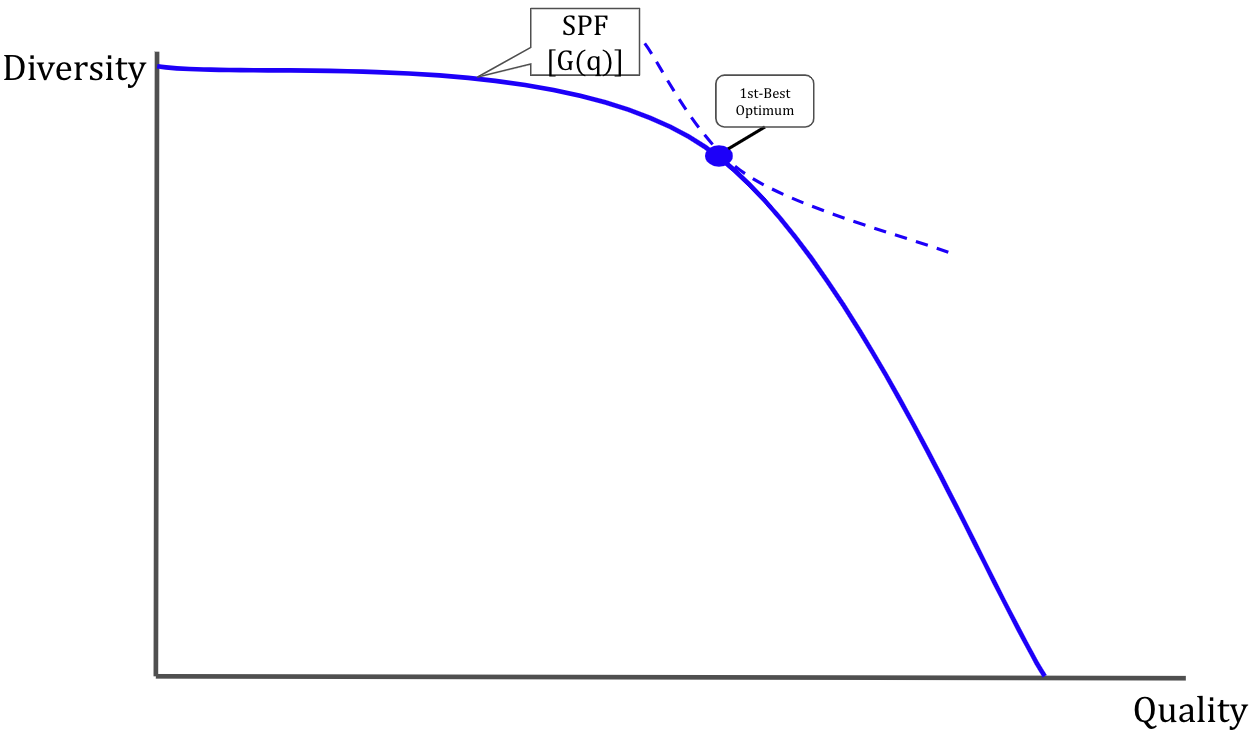
\includegraphics[width=1\textwidth,height=\textheight,keepaspectratio]{spf/model_spf.png} 
    \end{figure}
    
    \newpage
    \begin{figure}[!htb]
    \centering
        \caption{This figure depicts an example solution to an iteration of the selection problem with complexity induced search costs, which is described in Equation \ref{eq:objective}. As in Figure \ref{fig:model_spf}, the solid blue curve represents the SPF, the dotted blue curve represents the organization's indifference curve corresponding to the highest achievable utility without search costs, and the blue dot represents the diversity and performance of the first-best solution. Additionally, the solid red curve represents the accessible frontier with optimal search, the dotted red curve that represents the highest achievable utility with search costs, and the red dot that represents the diversity and performance of the optimal cohort with search costs (i.e. the second-best solution).}\label{fig:model_complex}
      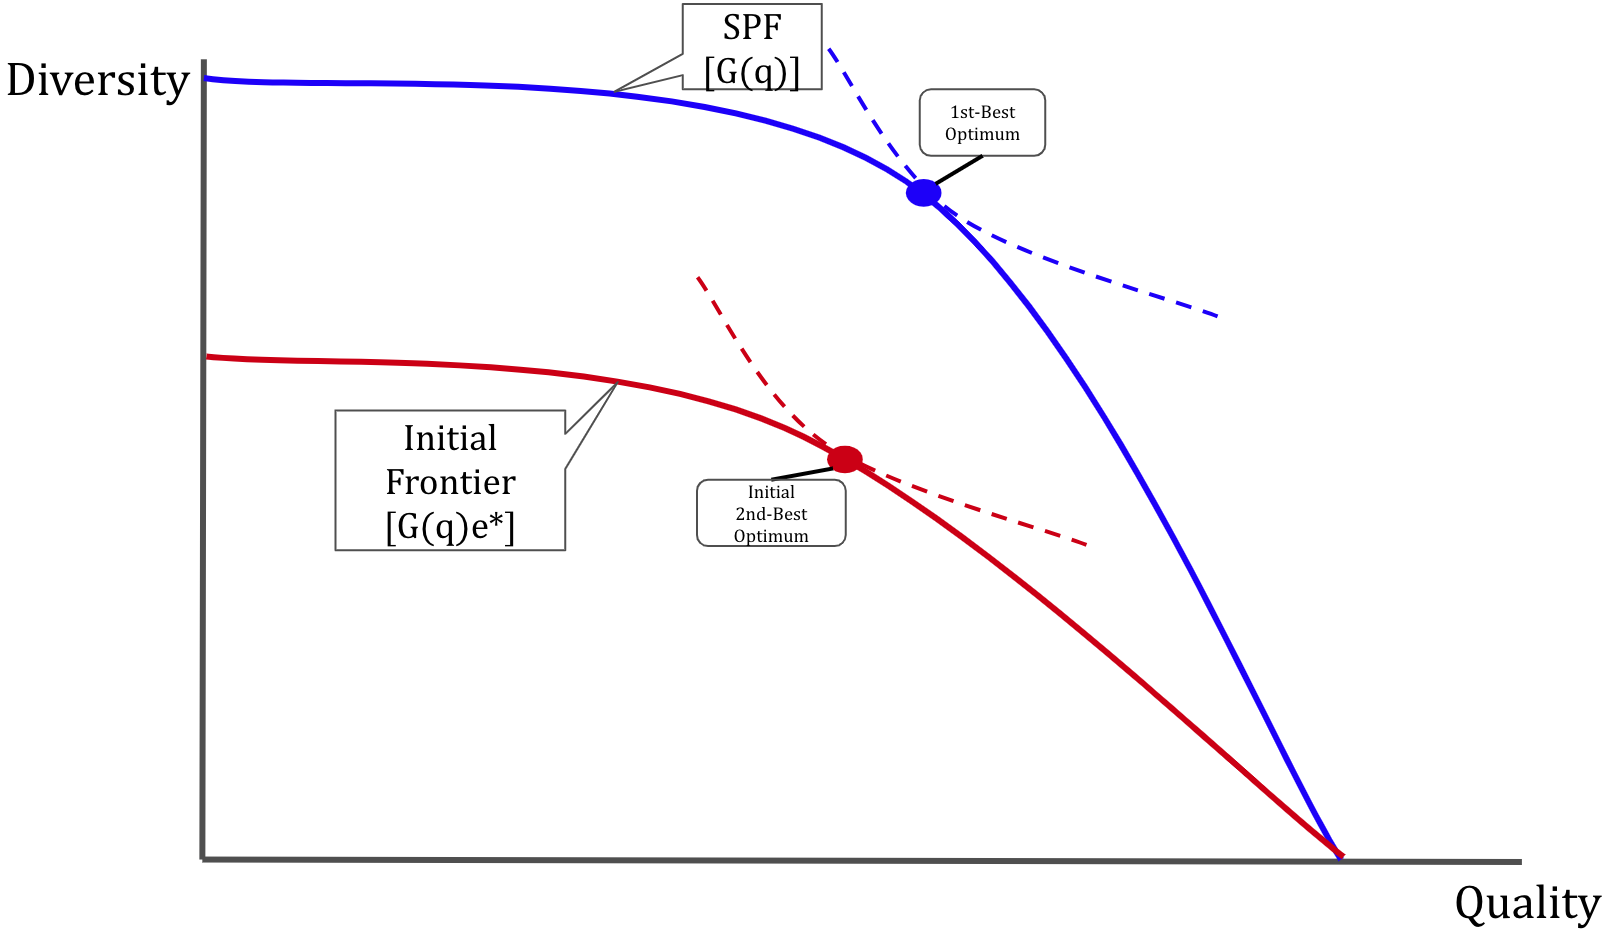
\includegraphics[width=1\textwidth,height=\textheight,keepaspectratio]{spf/model_complex.png} 
    \end{figure}
    
    \newpage
    \begin{figure}[!htb]
    \centering
        \caption{This figure depicts an example solution to an iteration of the selection problem with complexity induced search costs, which is described in Equation \ref{eq:objective}. As in Figure \ref{fig:model_spf}, the solid blue curve represents the SPF, the dotted blue curve represents the organization's indifference curve corresponding to the highest achievable utility without search costs, and the blue dot represents the diversity and performance of the first-best solution. And, as in \ref{fig:model_spf}, the solid red curve represents the accessible frontier with optimal search, the dotted red curve that represents the highest achievable utility with search costs, and the red dot that represents the diversity and performance of the second-best cohort with poor search technology (i.e. high $\alpha$). And, the green curves and dot represent the SPF estimate that is accessible with an improved search technology and new second-best solution, respectively. The difference between the initial second-best solution and the new solution is a graphical representation of the implications of the comparative static signed in Equation \ref{eq:comp_stat} ($\frac{\partial e^*}{\partial \alpha}$).}\label{fig:model_spf_est}
      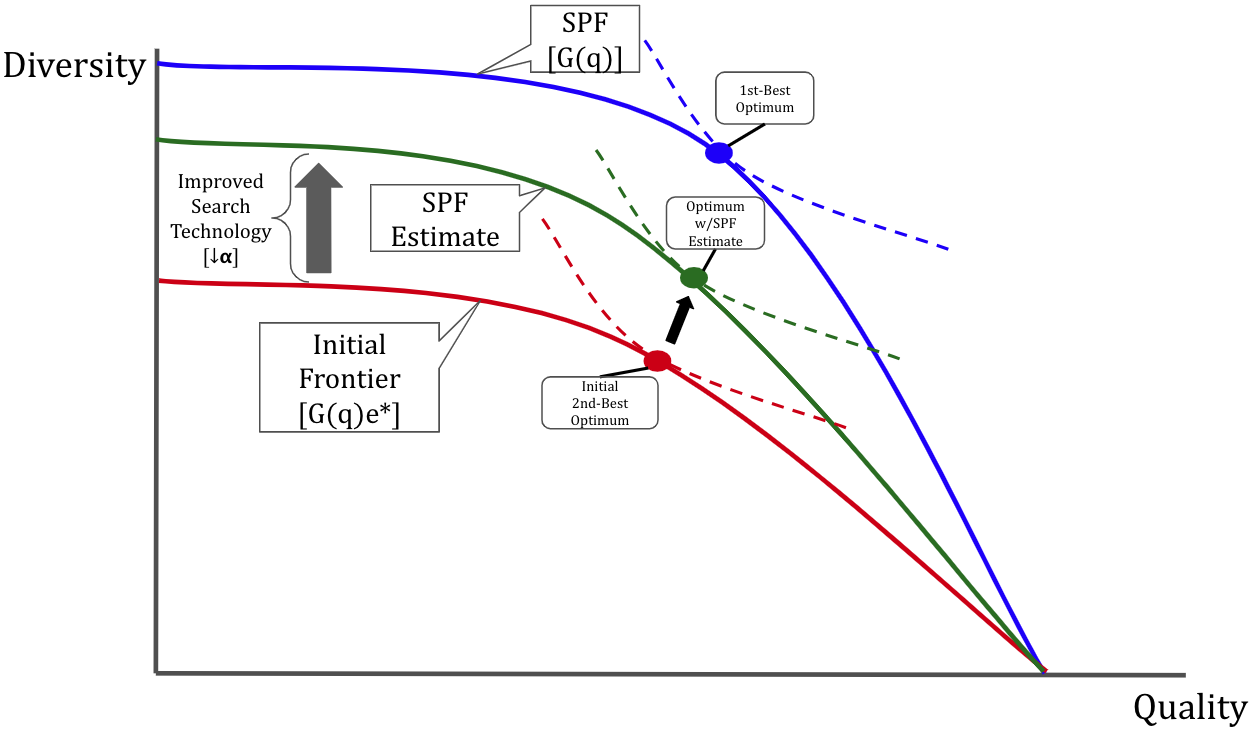
\includegraphics[width=1\textwidth,height=\textheight,keepaspectratio]{spf/model_spf_est.png}
    \end{figure}
    
    
    \newpage
    \null %The \null -> \vfill -> figure code -> \vfill code centers the figure vertically on the page
    \vfill
    \begin{center}
    \begin{figure}[!htb]
    \centering
        \caption{This figure schematizes the key elements of the talent investment program's data collection and selection process. }\label{fig:design}
      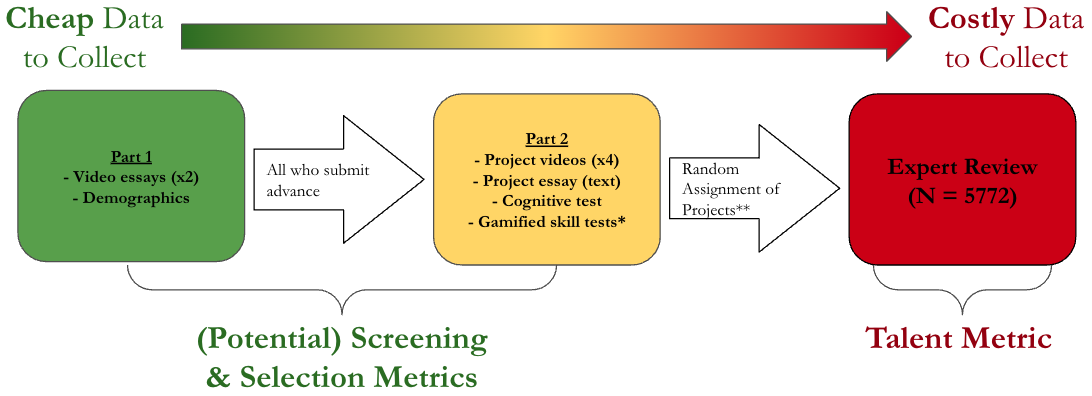
\includegraphics[width=\textwidth,height=\textheight,keepaspectratio]{background/selection_design_schematic.png} 
    \end{figure}
    \end{center}
    \vfill
    
    
    \newpage
    
    \begin{figure}[!htb]
    \centering
        \caption{Distribution of Applicant Countries Data come from surveys completed by applicants. Data are pooled across all three application cohorts. Overall applicants come from 153 different countries. The distribution of proportions of applicants by country in this figure are limited to the 50 countries from which there were the most applicants. The top 5 countries are labeled on the figure.  }\label{fig:country_dist_all}
      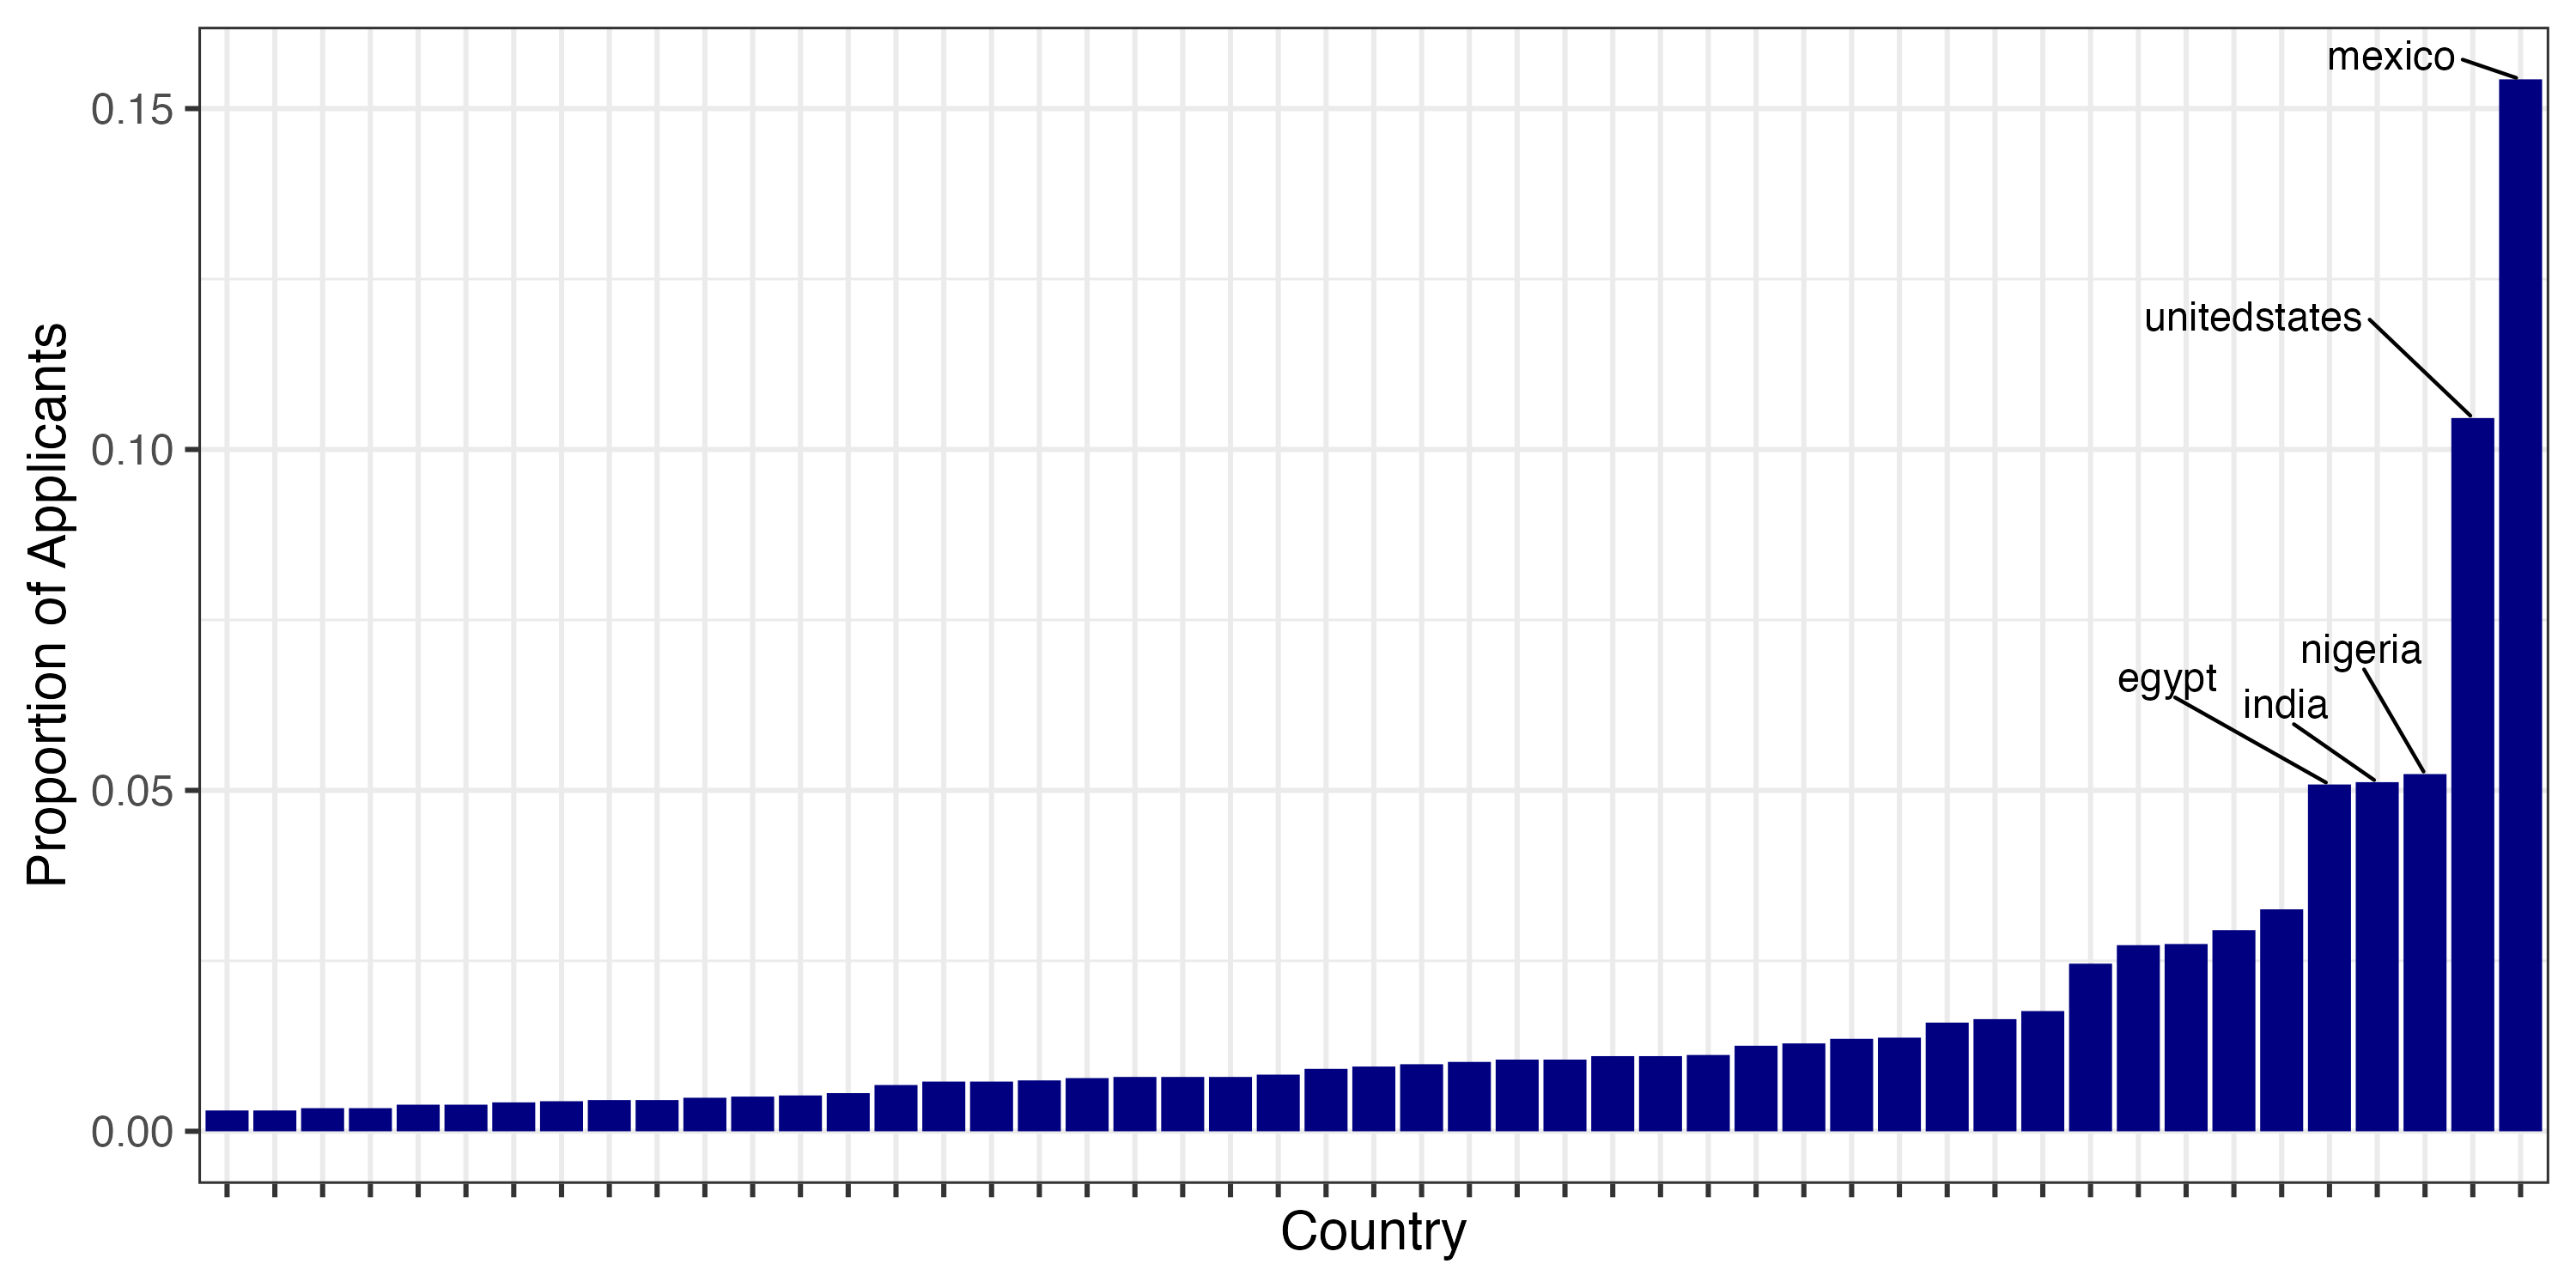
\includegraphics[width=1.3\textwidth,height=\textheight,keepaspectratio]{spf/candidate_countries.png} 
    \end{figure}
    
    
    \begin{figure}[!htb]
        \centering
        \caption{Distributions of Applicant Project Topics and Reviewer Expertise. Data come from surveys completed by applicants. Data are pooled across all three application cohorts. Panel (\ref{subfig:app_proj_topics}) depicts the proportion of all applicant projects in each topic category. Panel (\ref{subfig:rev_expertise}) depicts the proportion of project reviewers with each category of expertise.} \label{fig:topic_expertise_dist}
        \begin{subfigure}[t]{\textwidth}
            \centering
                    \caption{Applicant Project Topics} \label{subfig:app_proj_topics}
            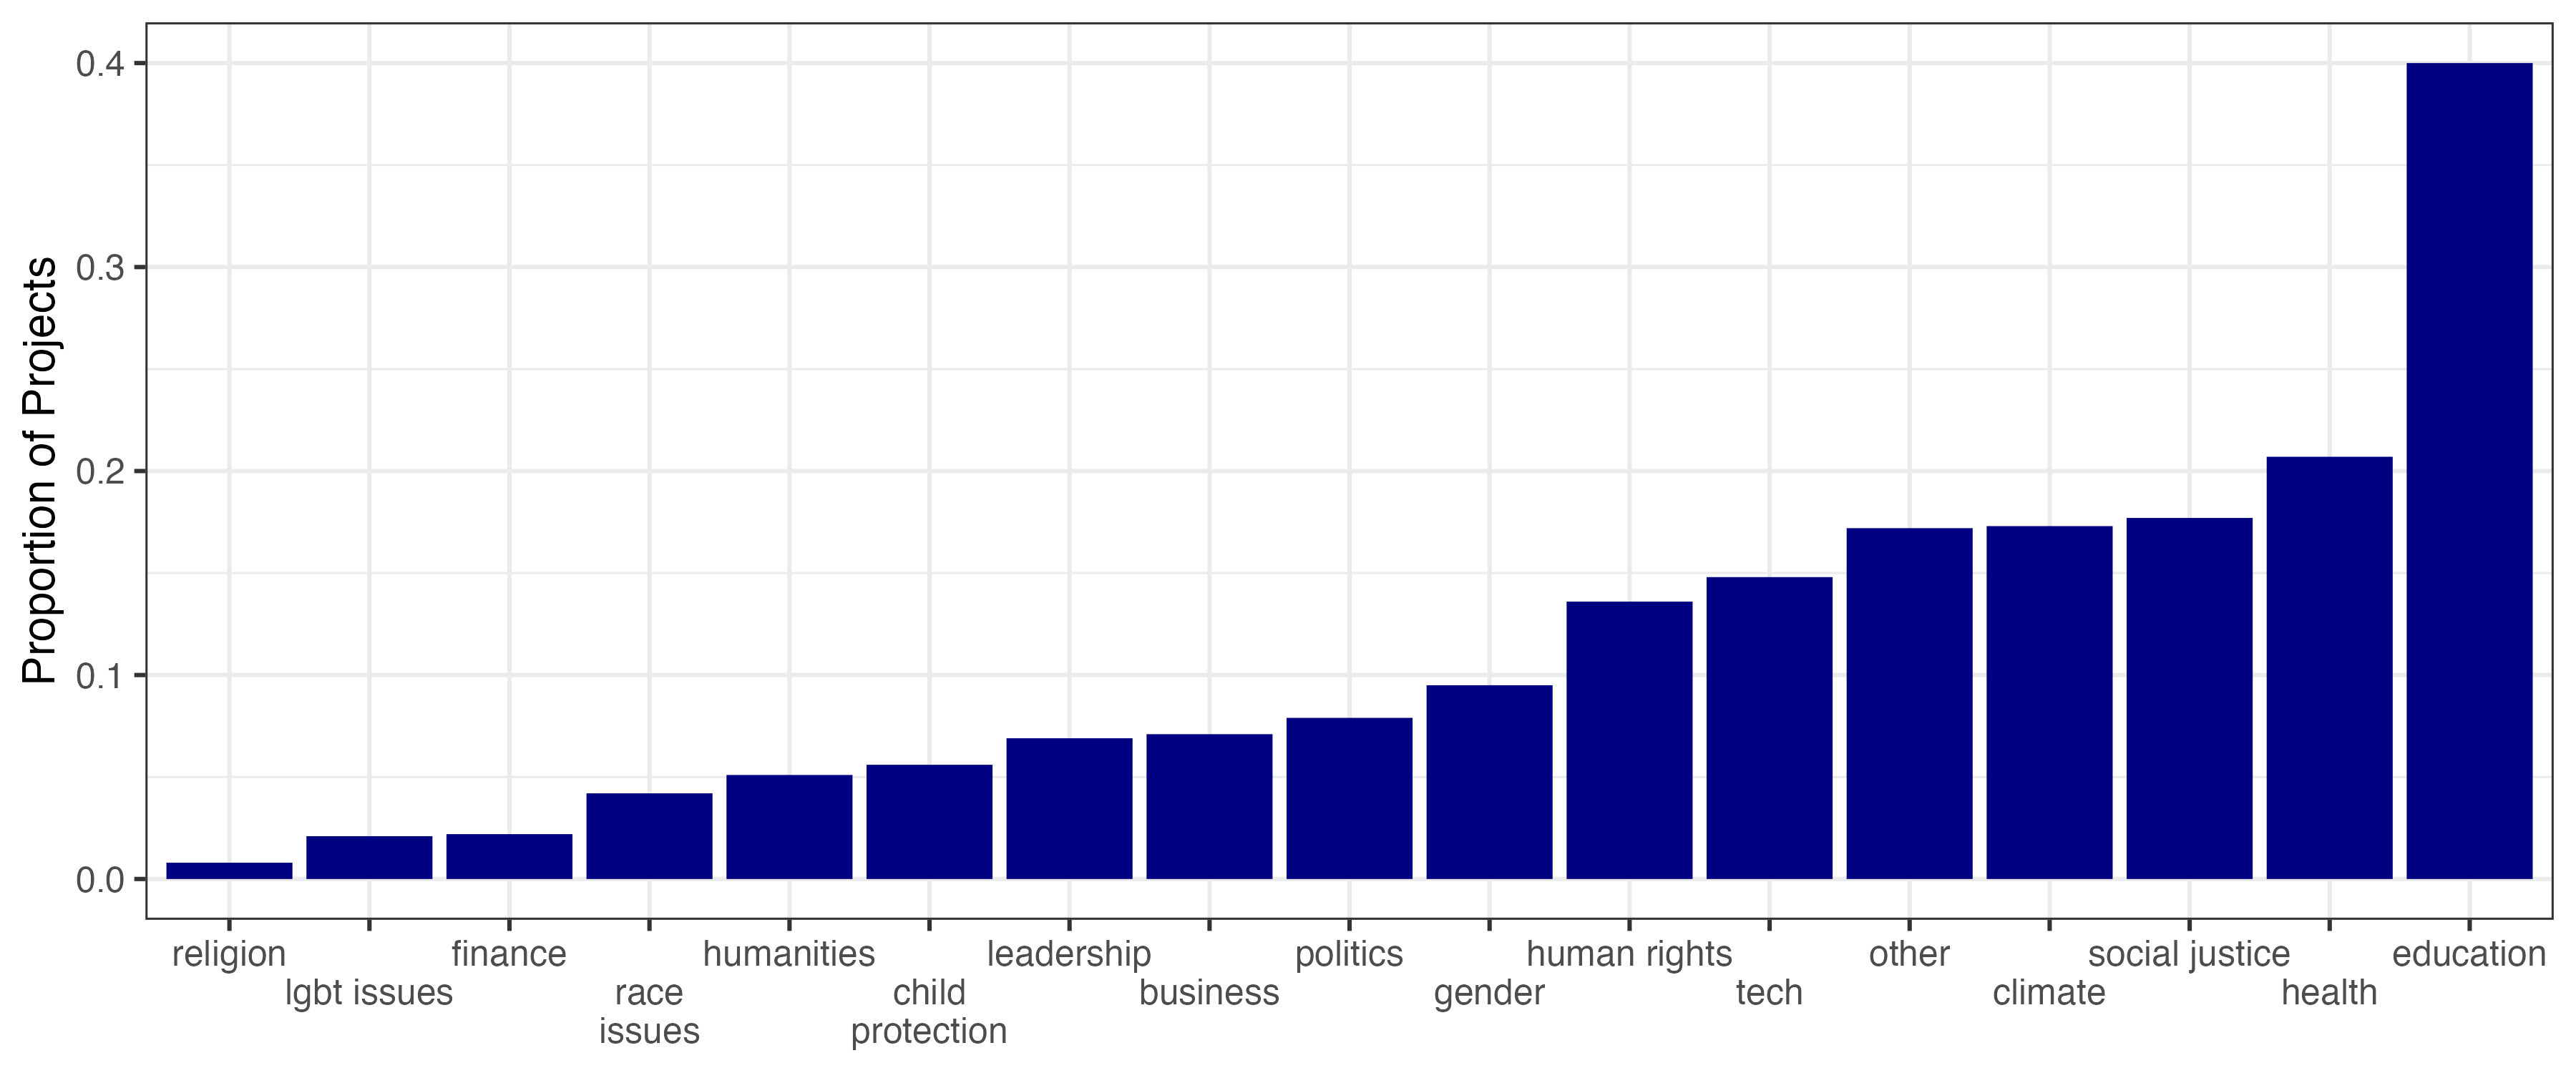
\includegraphics[width=\linewidth]{spf/applicant_project_topics.png} 
        \end{subfigure}
        \hfill
        \vspace{1em}
        \begin{subfigure}[t]{\textwidth}
            \centering
                   \caption{Reviewer Areas of Expertise} \label{subfig:rev_expertise}
            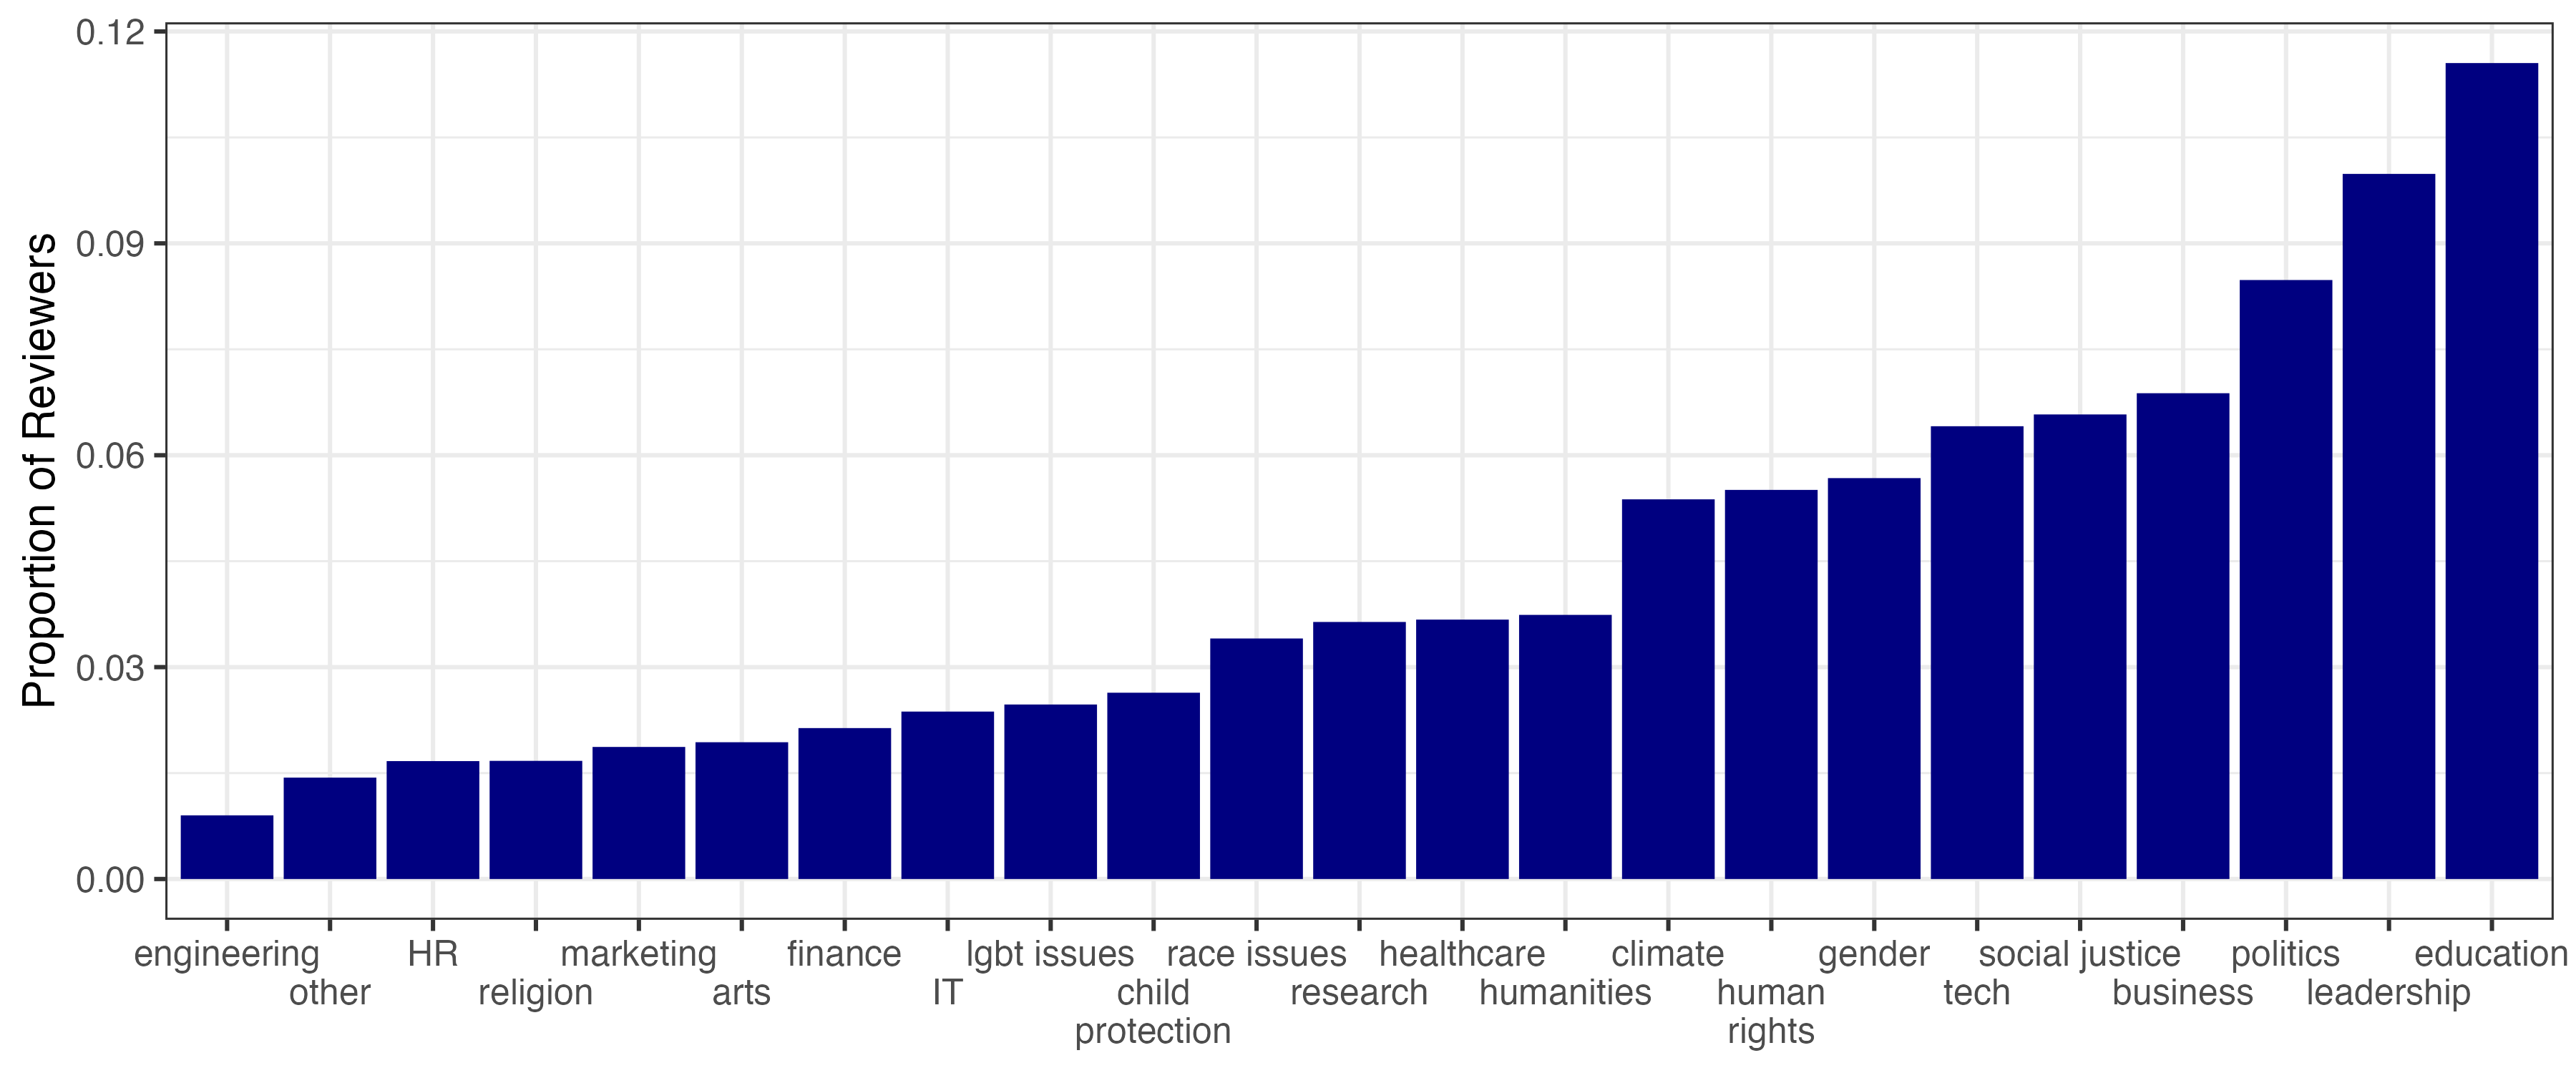
\includegraphics[width=\linewidth]{spf/reviewer_expertise.png} 
        \end{subfigure}
    \end{figure}
    
    
    \begin{figure}[!htb]
        \centering
        \caption{Distributions of Reviewer Industries and Organizations (Cycle 1). Data come from surveys completed by applicants. Data come from application cycle 1 only (industry and organization information were not collected for the in cycles 2 and 3). Panel (\ref{subfig:rev_industries}) depicts the proportion of all project reviewers by industries. Unfortunately, industries were not categorized using standard codes, but the categories are decipherable. Panel (\ref{subfig:rev_orgs}) depicts the proportion of project reviewers from each organization that referred them. The top two most common referring organizations make up 46\% of all expert reviewers, and the labels on them have been redacted to maintain the program's anonymity. }
        \begin{subfigure}[t]{\textwidth}
            \centering
                    \caption{Industries} \label{subfig:rev_industries}
            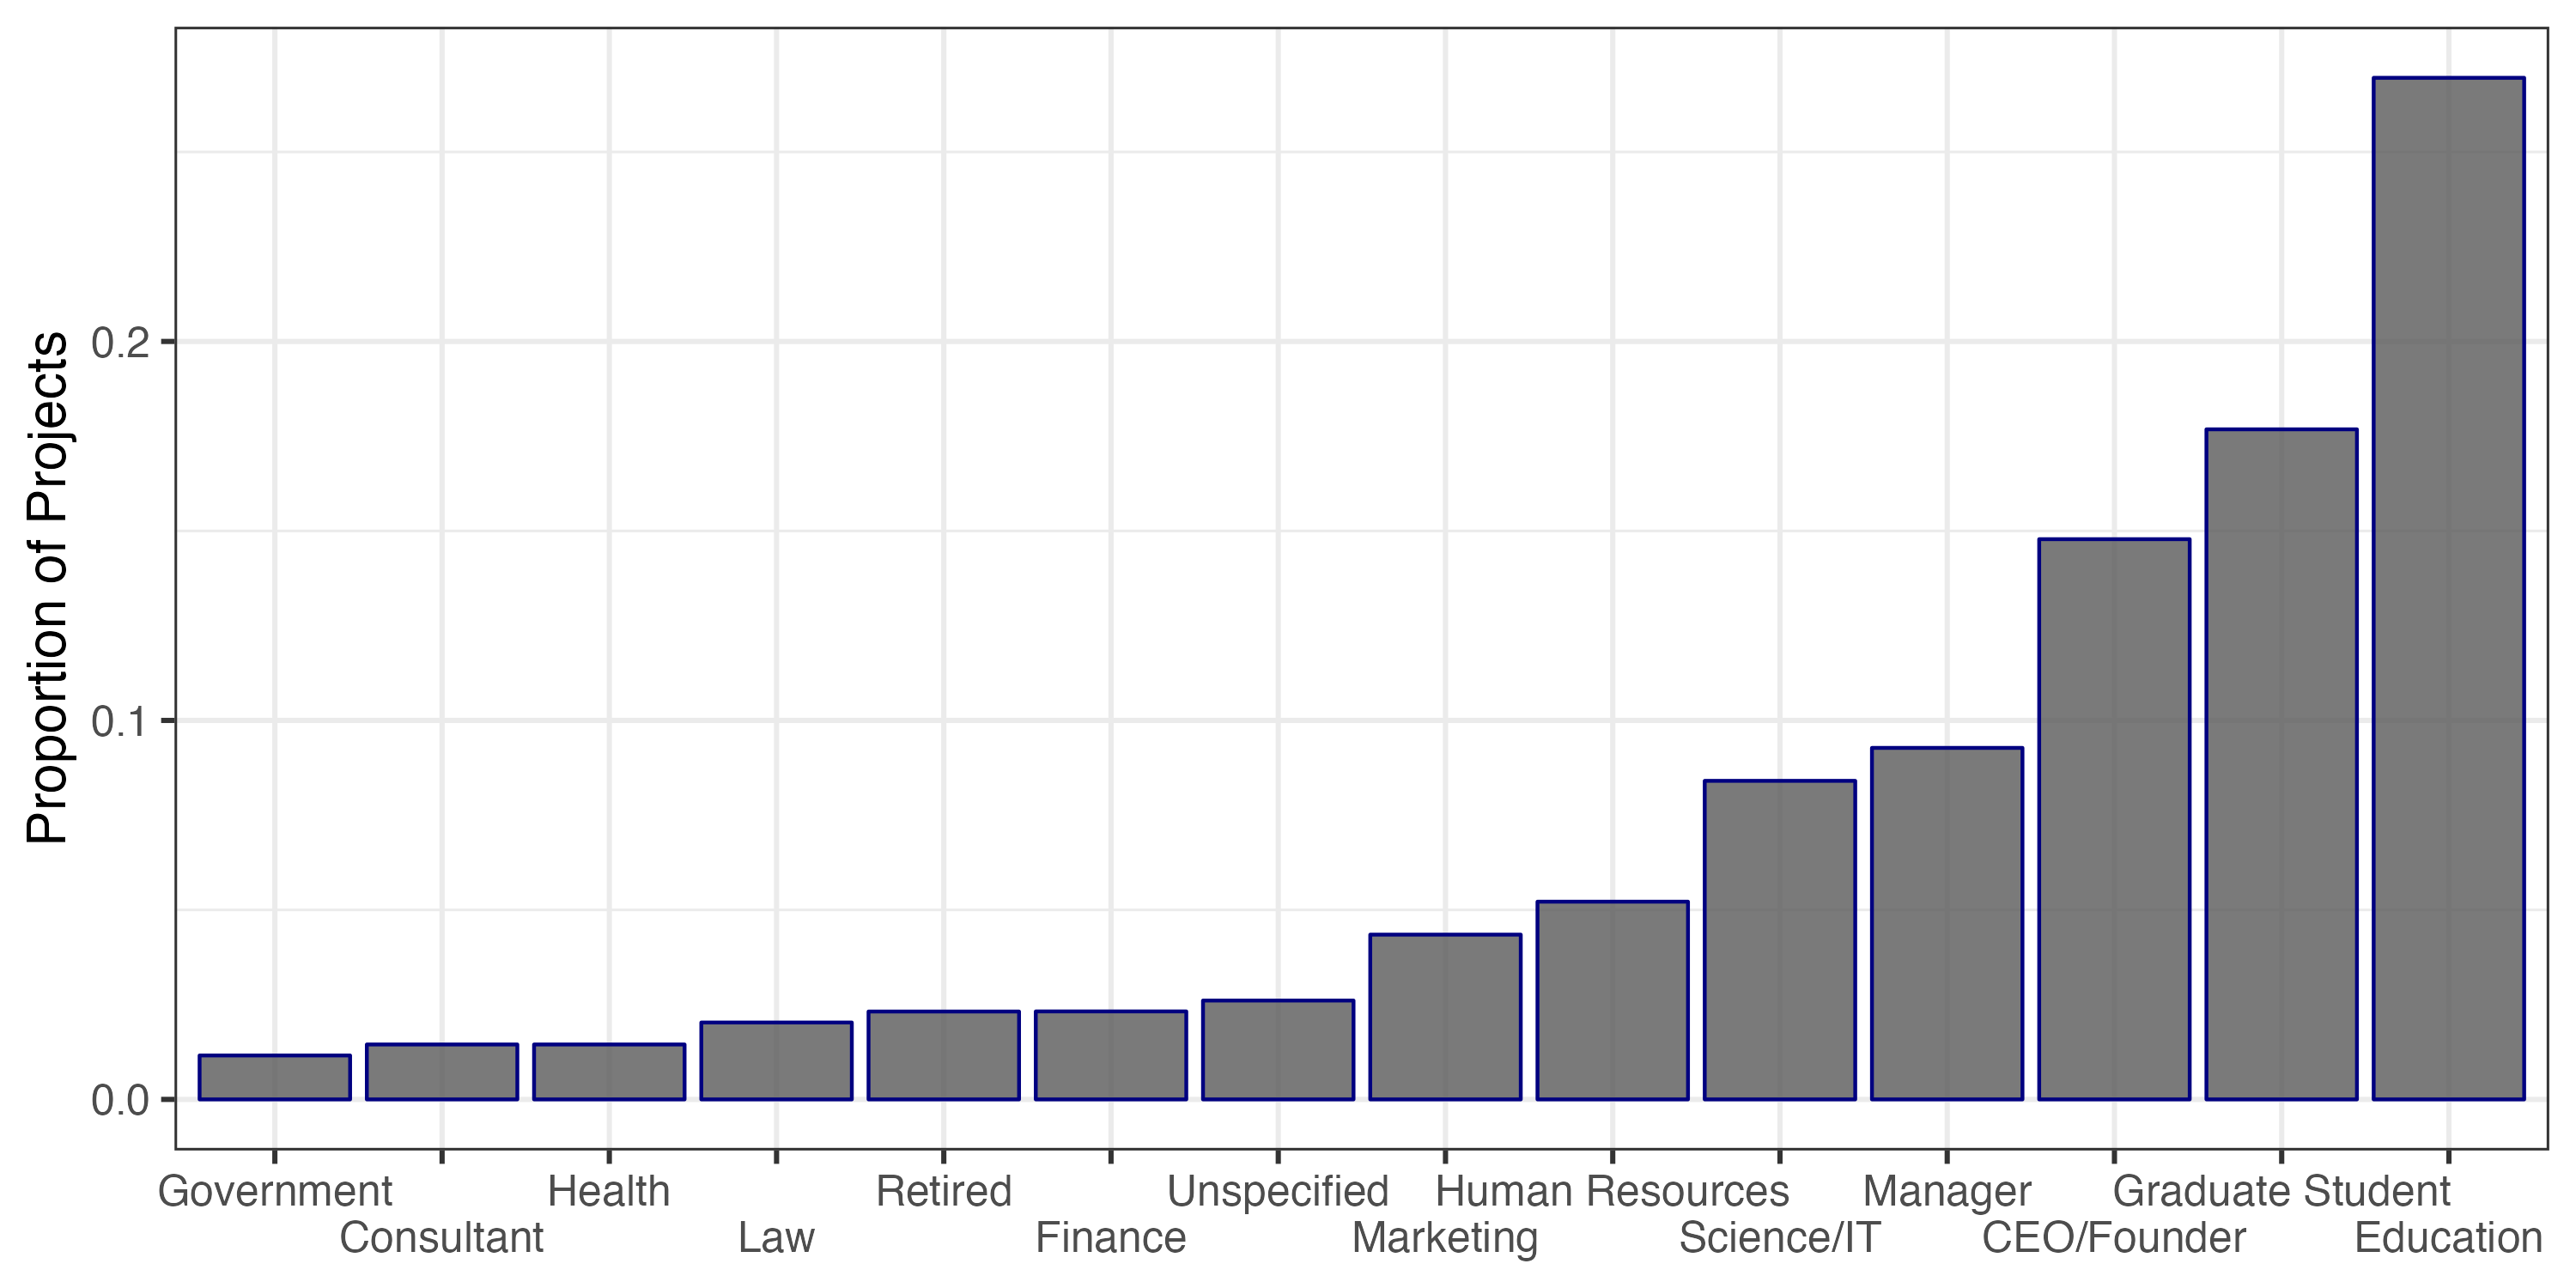
\includegraphics[width=\linewidth]{spf/project_reviewer_industries.png} 
        \end{subfigure}
        \hfill
        \vspace{1em}
        \begin{subfigure}[t]{\textwidth}
            \centering
                   \caption{Organizations (Top 2 Labeled)} \label{subfig:rev_orgs}
            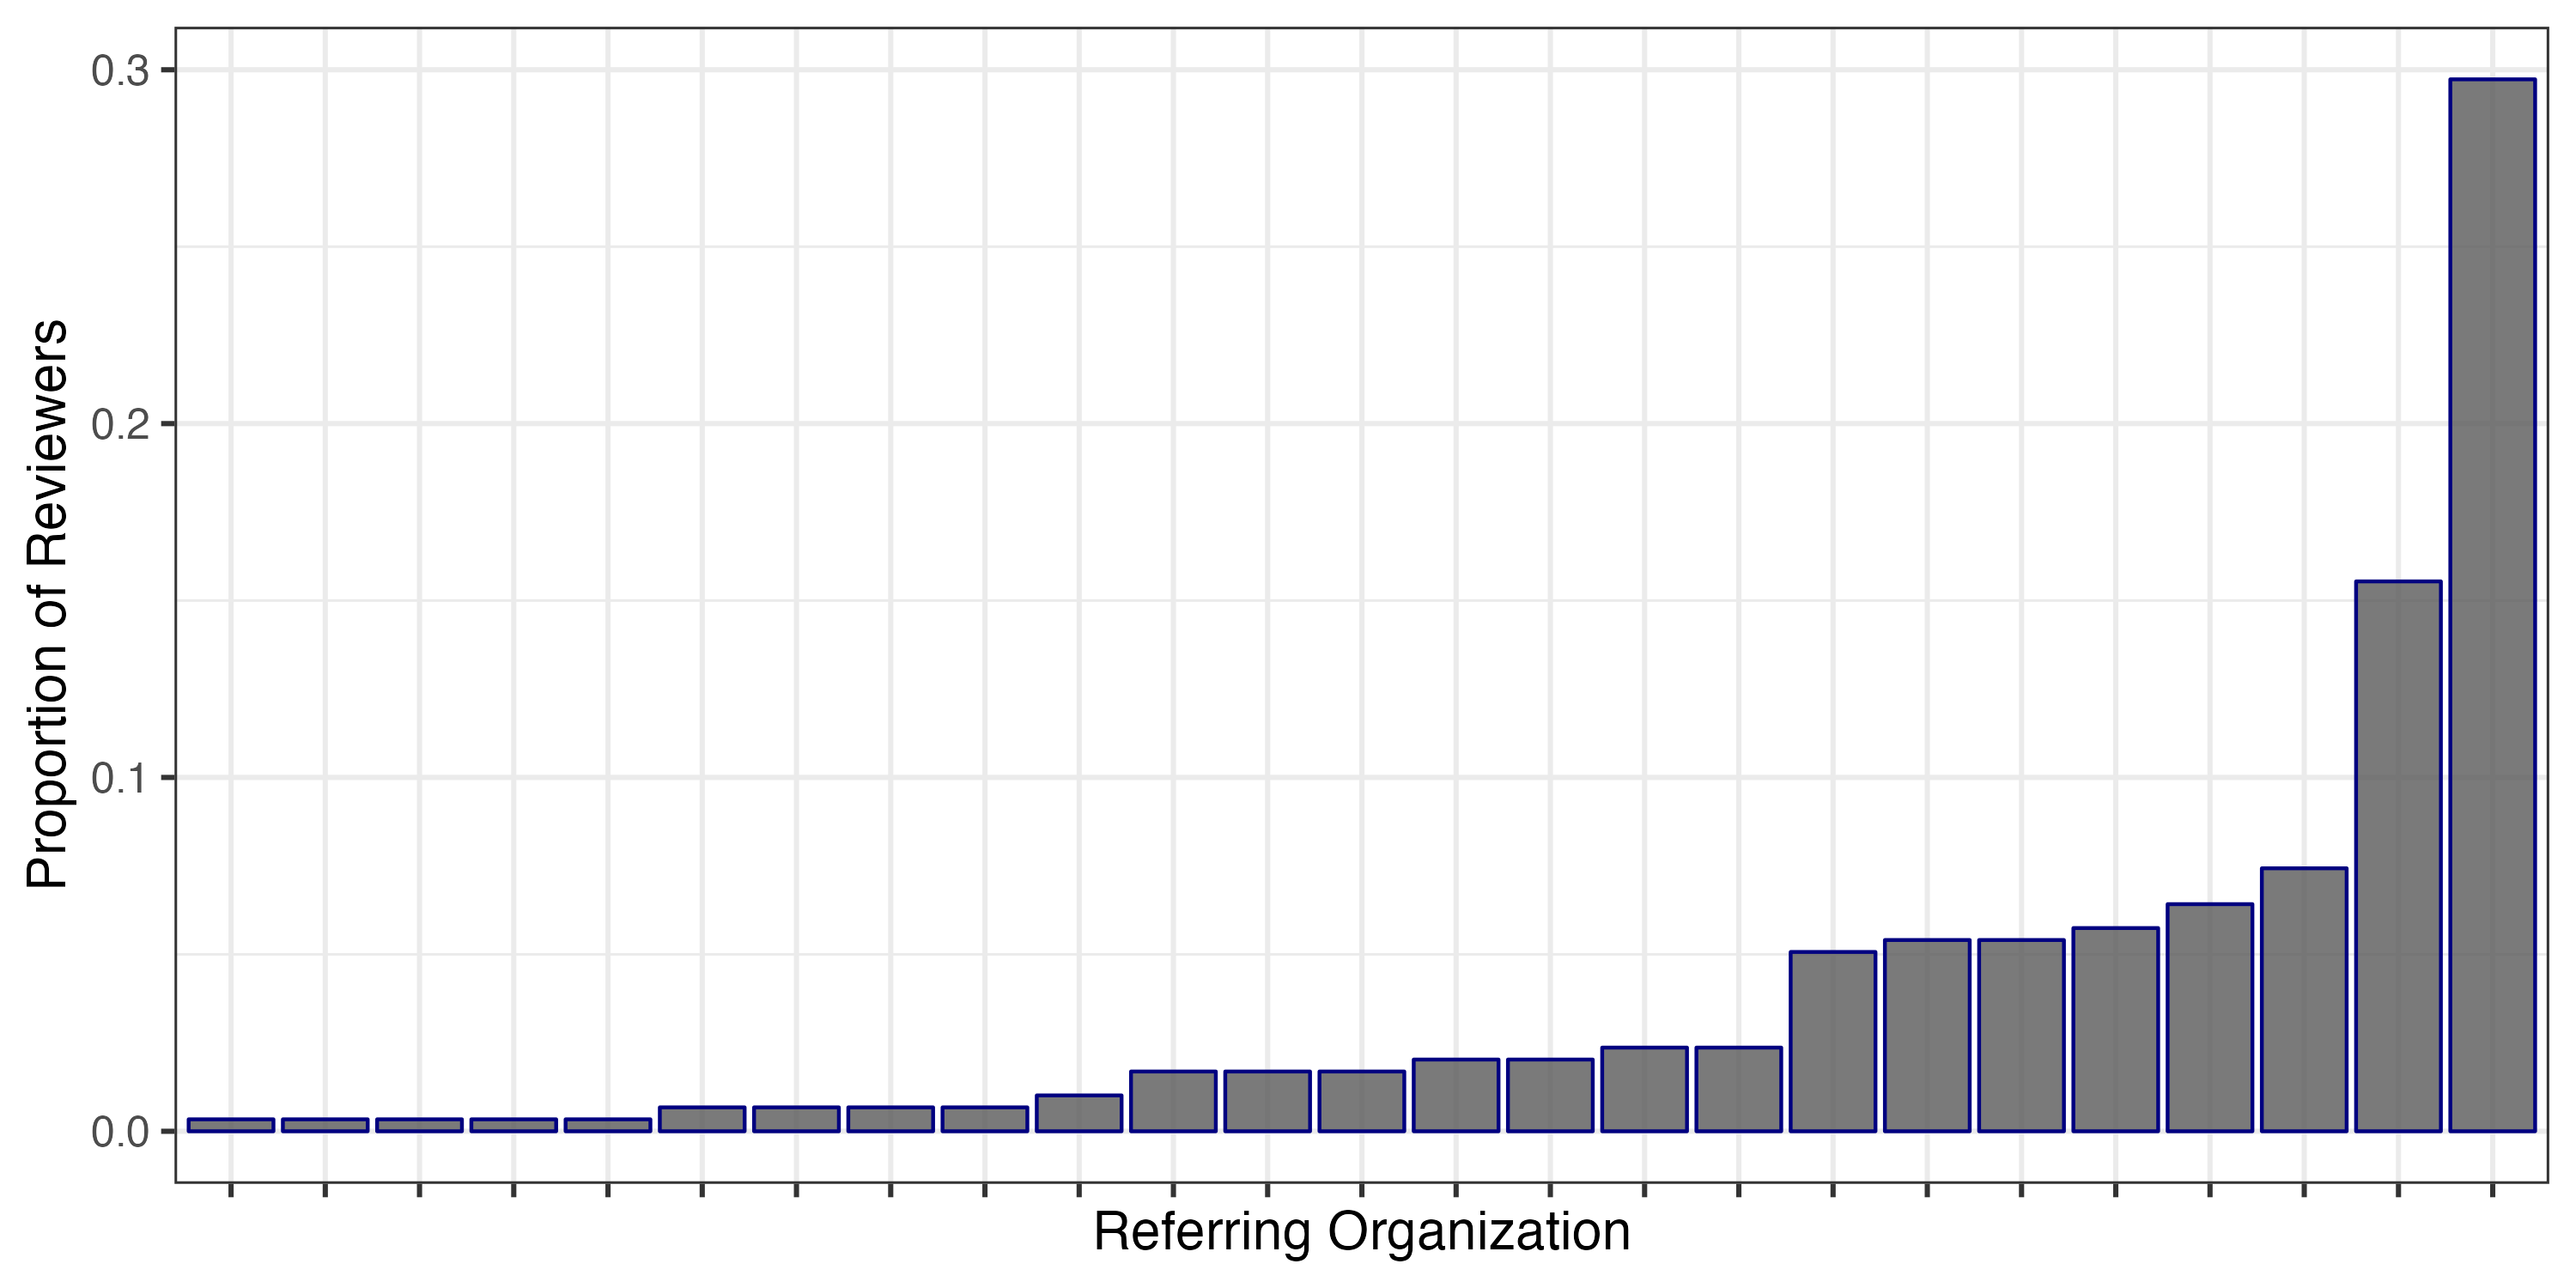
\includegraphics[width=\linewidth]{spf/project_reviewer_affiliations.png} 
        \end{subfigure}
    \end{figure}
    
    \newpage
    \begin{figure}[!htb]
    \centering
        \caption{This figure displays the SPF we estimate for the cycle 1 finalist cohort. The y-axis represents the diversity score while the x-axis represents average cohort performance (i.e. project scores). The green curve is our estimate of the cycle 1 SPF, which represents the upper bound of diversity that is achievable at every level of cohort performance. The red dot depicts the actual level of diversity and performance of the finalists that were selected in cycle 1. The vertical and horizontal dashed red lines represent the maximum Pareto gain that was possible along the diversity and performance dimensions respectively. In particular, cohort diversity could have been improved by 15.2\% without any reduction in cohort performance. And, cohort performance could have been improved by 15.6\% without any cost to diversity. } \label{fig:spf_2021}
      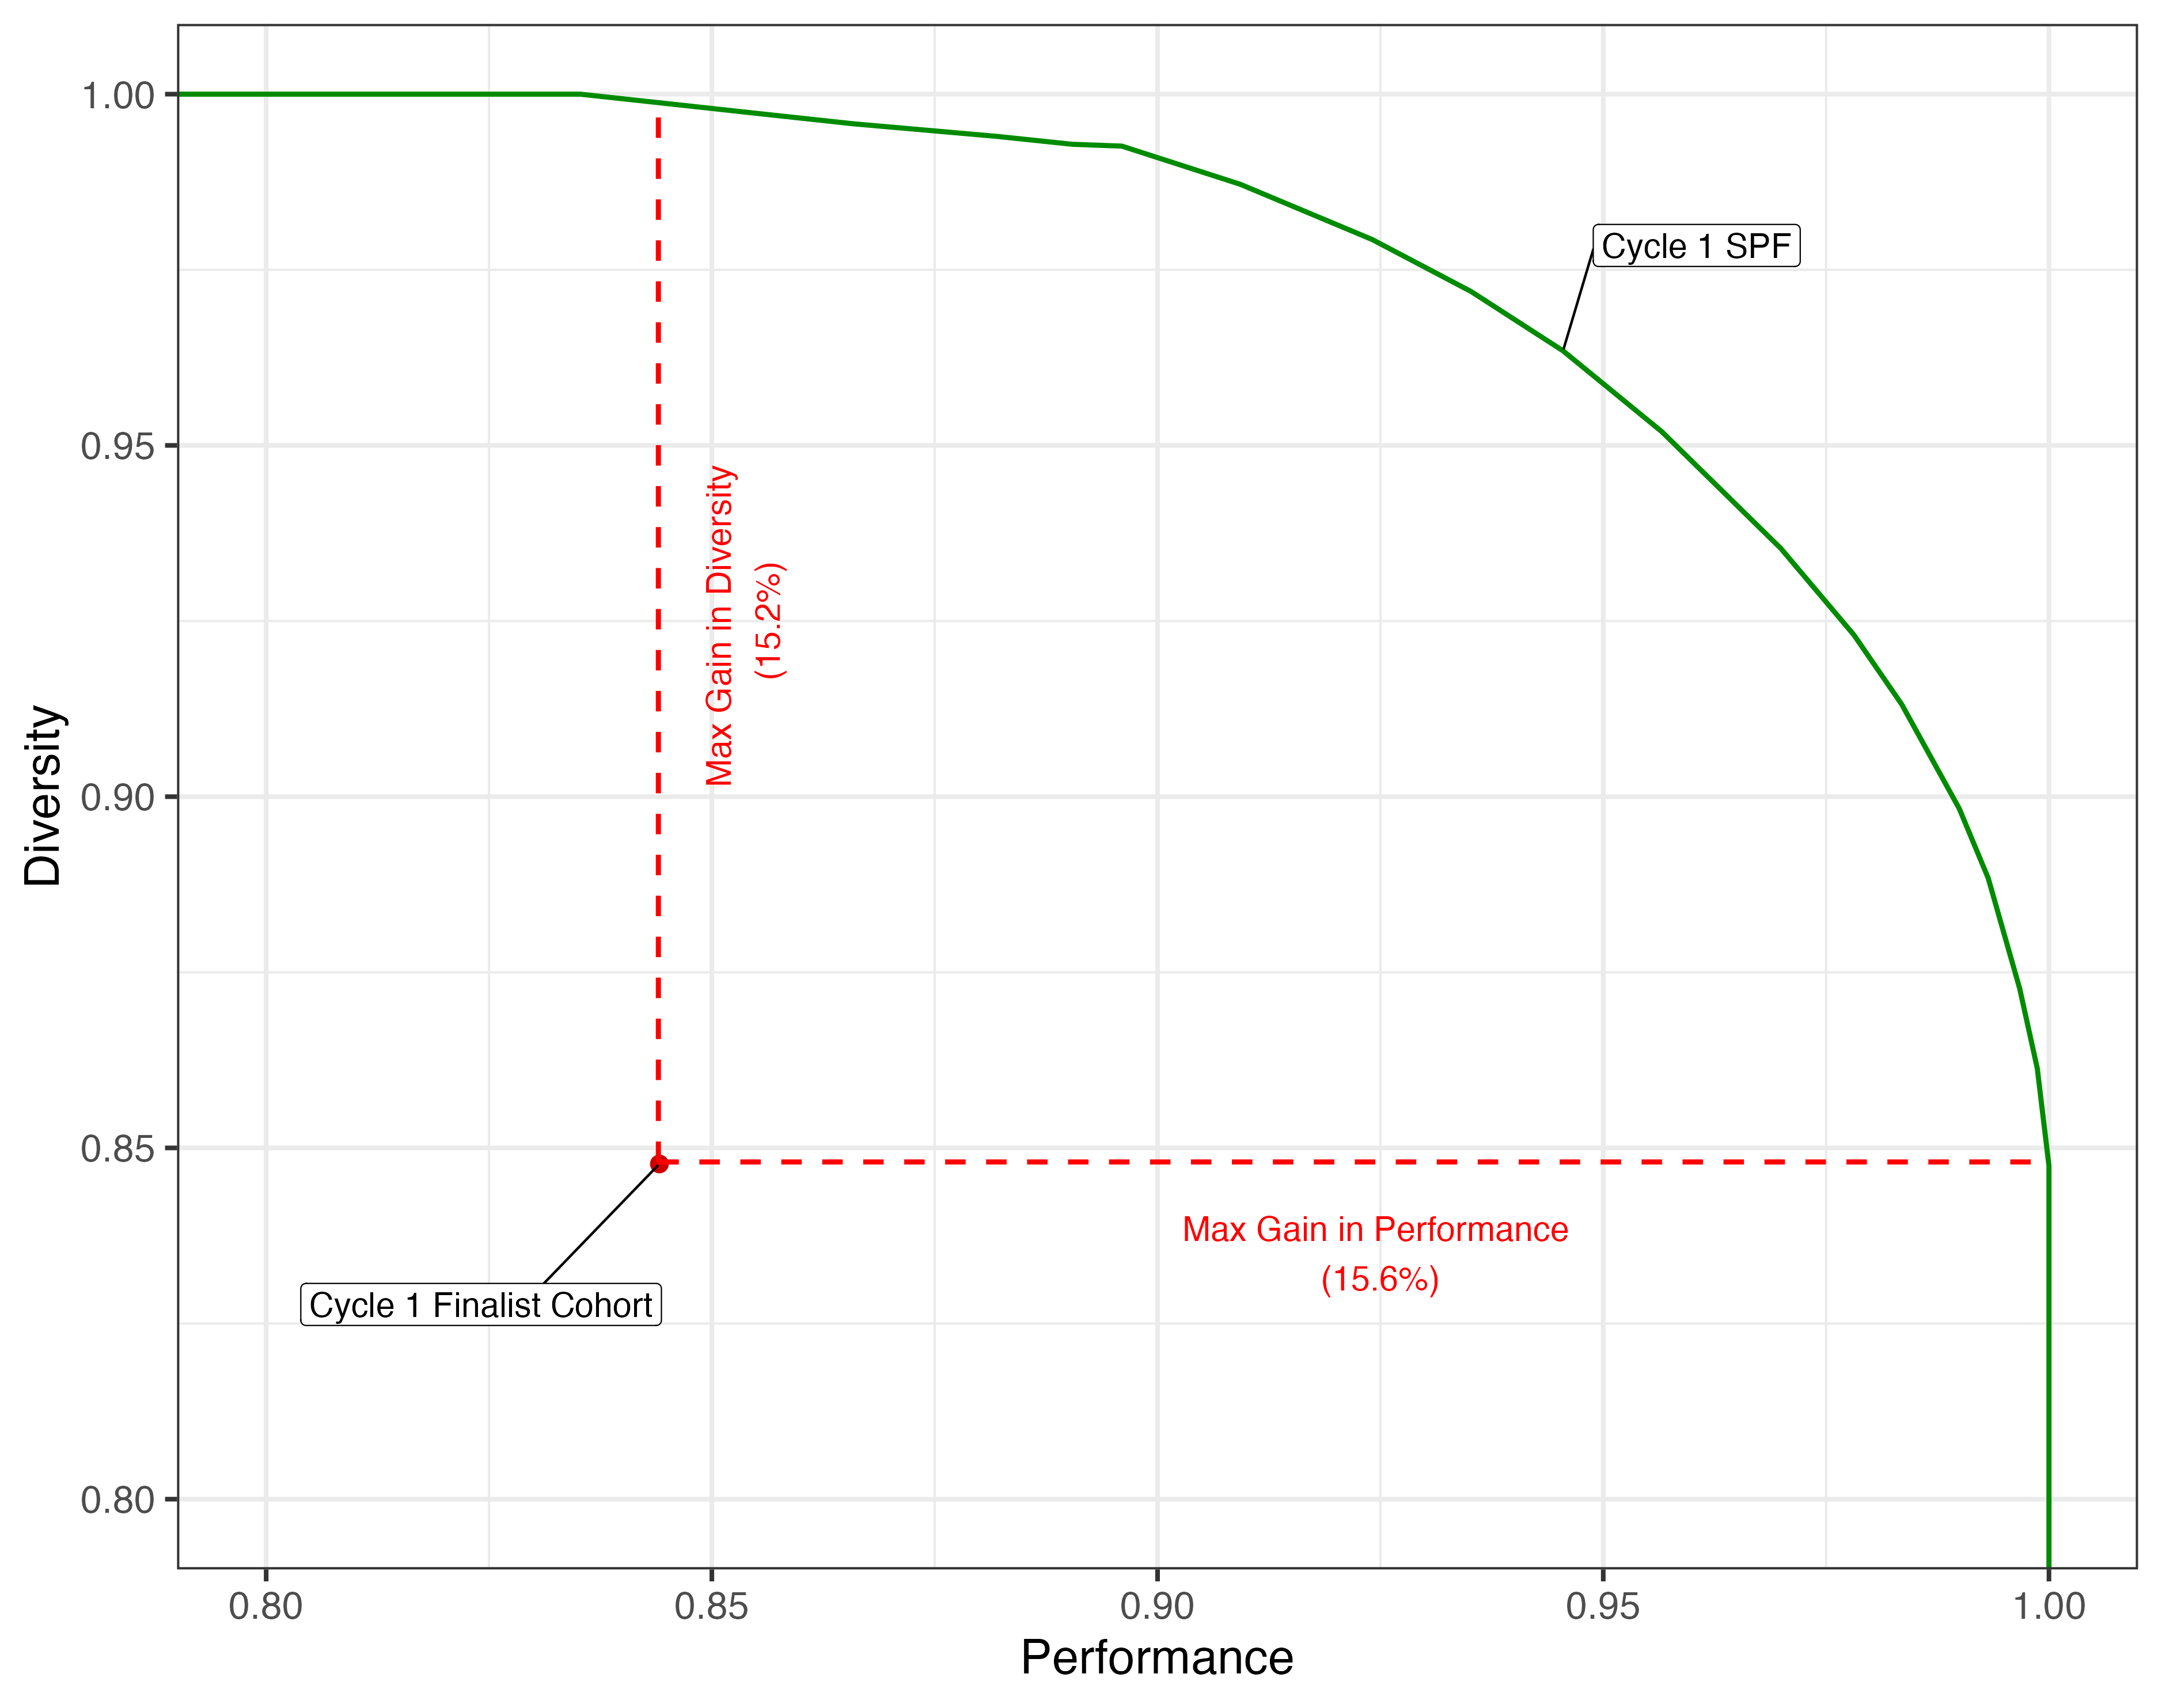
\includegraphics[width=\textwidth,height=\textheight,keepaspectratio]{spf/yr1_spf_finalist.png} 
    \end{figure}
    
    \newpage
    \begin{figure}[!htb]
    \centering
        \caption{This figure displays the SPF we estimate for the cycle 2 finalist cohort. The y-axis represents the diversity score while the x-axis represents average cohort performance (i.e. project scores). The green curve is our estimate of the cycle SPF, which represents the upper bound of diversity that is achievable at every level of cohort performance. The red dot depicts the actual level of diversity and performance of the finalists that were selected in cycle 2. The vertical and horizontal dashed red lines represent the maximum Pareto gain that was possible along the diversity and performance dimensions respectively. In particular, cohort diversity could have been improved by 13\% without any reduction in cohort performance. And, cohort performance could have been improved by 19.6\% without any cost to diversity. } \label{fig:spf_2022}
      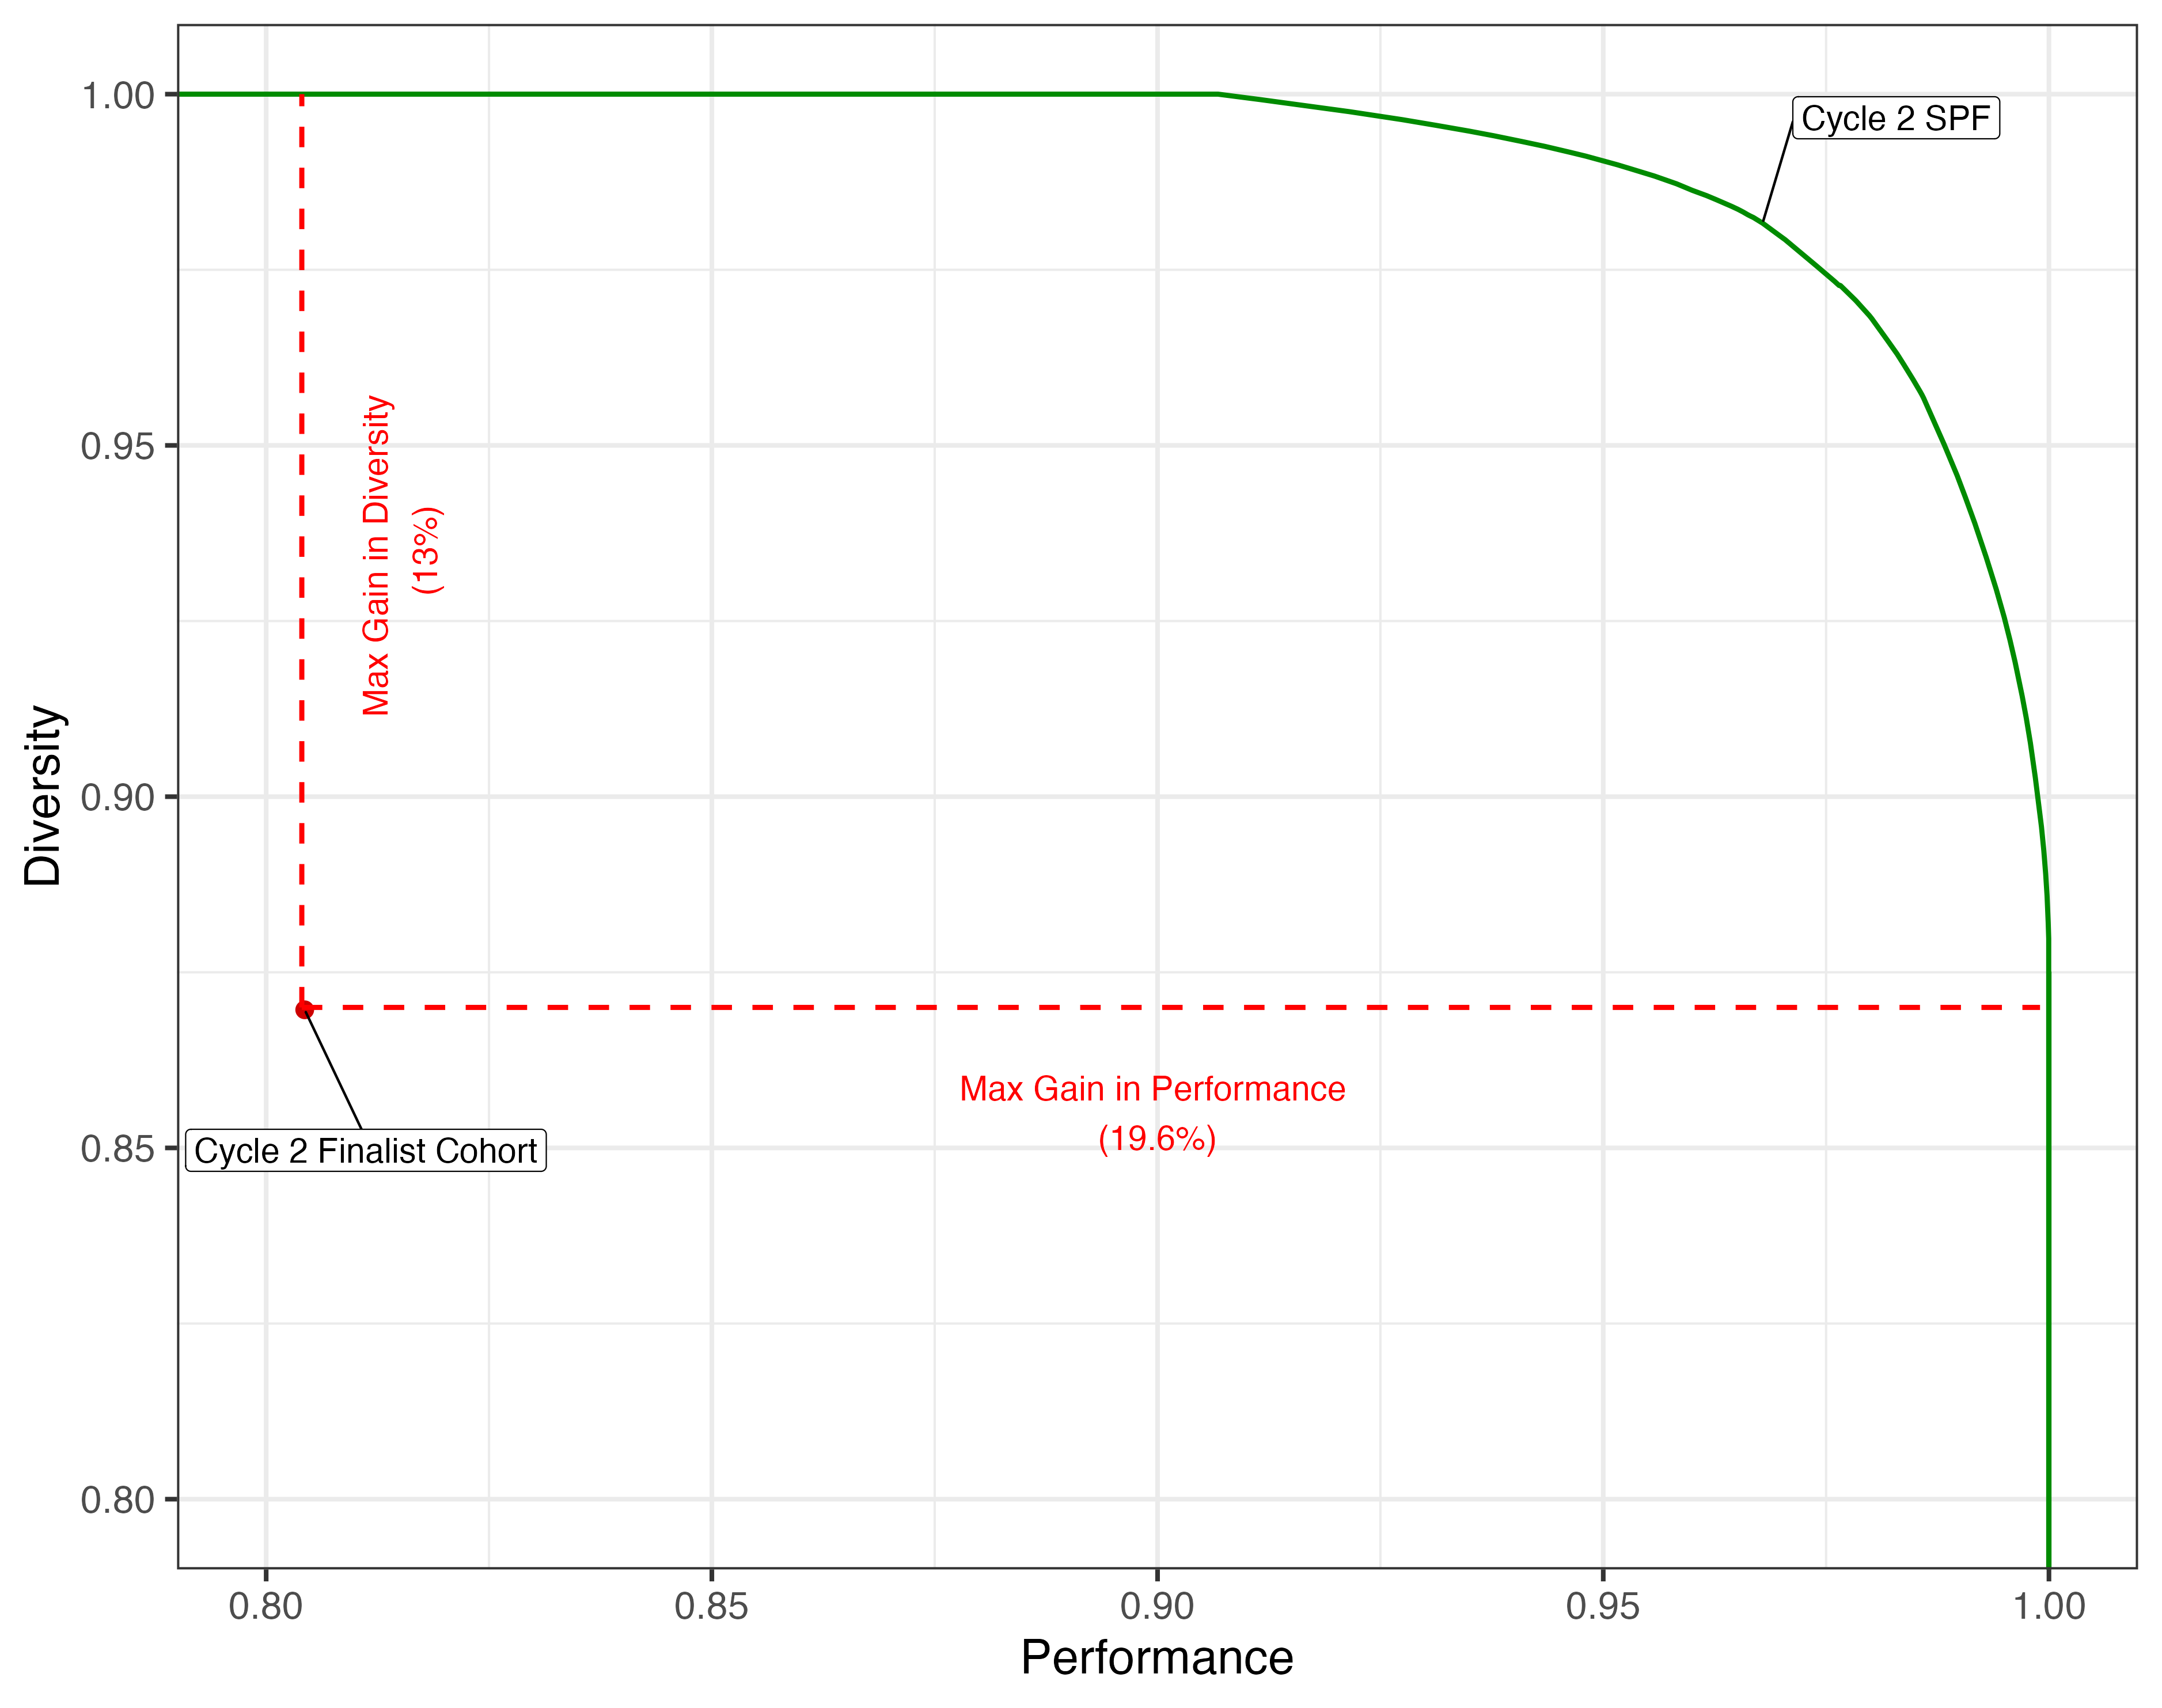
\includegraphics[width=\textwidth,height=\textheight,keepaspectratio]{spf/yr2_spf_finalist.png} 
    \end{figure}
    
    \newpage
    \begin{figure}[!htb]
    \centering
        \caption{This figure displays the SPF we estimate for the cycle 3 finalist cohort. The y-axis represents the diversity score while the x-axis represents average cohort performance (i.e. project scores). The green curve is our estimate of the cycle 3 SPF, which represents the upper bound of diversity that is achievable at every level of cohort performance.The red dots depict the actual level of diversity and performance of the finalists that were selected in cycles 1-3, respectively. The diagonal dashed red line represents the distance in diversity-performance space between the cycle 2 cohort and the cycle 3 cohort. In cycle 3, there are no significant Pareto improvements on either diversity or performance. } \label{fig:spf_2023}
      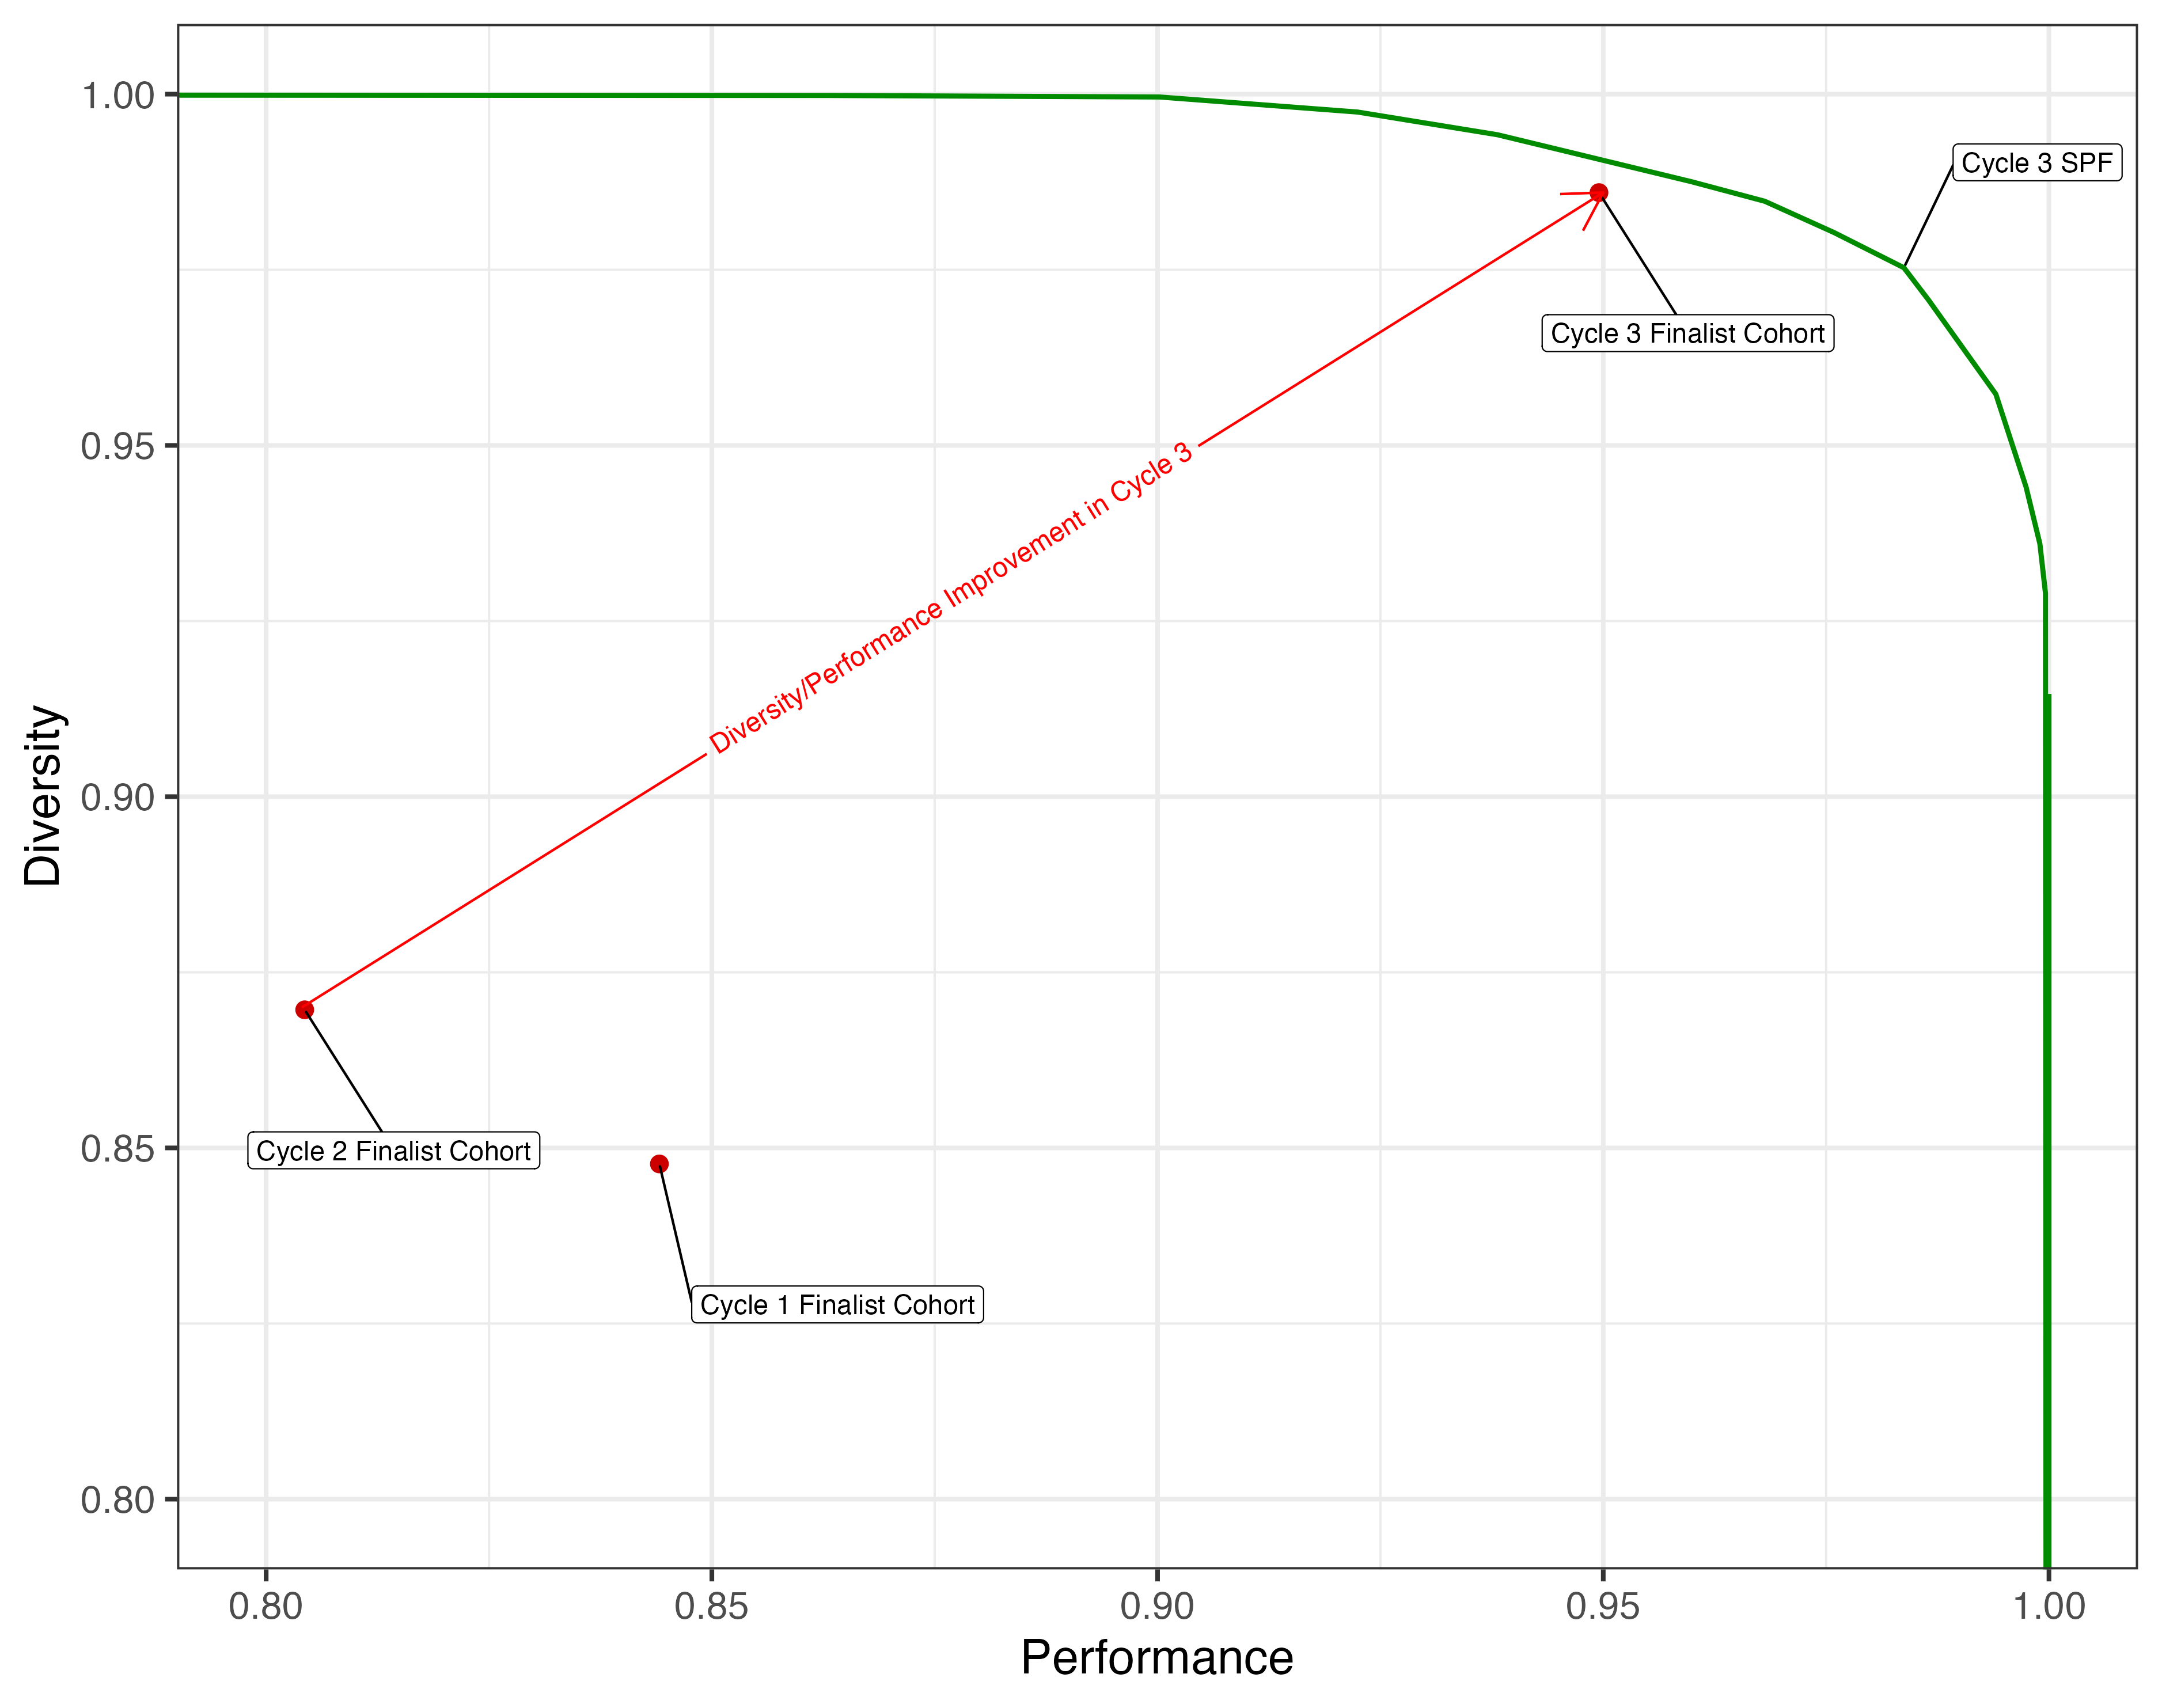
\includegraphics[width=\textwidth,height=\textheight,keepaspectratio]{spf/yr3_spf_finalist.png} 
    \end{figure}
    
    
    \newpage
    \begin{figure}[!htb]
    \centering
        \caption{This figure displays permutations tests of the distributions of differences in project performance (panel a) and diversity (panel b) from 1000 randomly drawn pairs of potential cohorts from application cycle 1. The dashed black vertical line represents the 95 percentile of these differences. The solid vertical lines represent the max pareto gain on performance (panel a) and diversity (panel b) in each application year.} \label{fig:permutation_tests}
      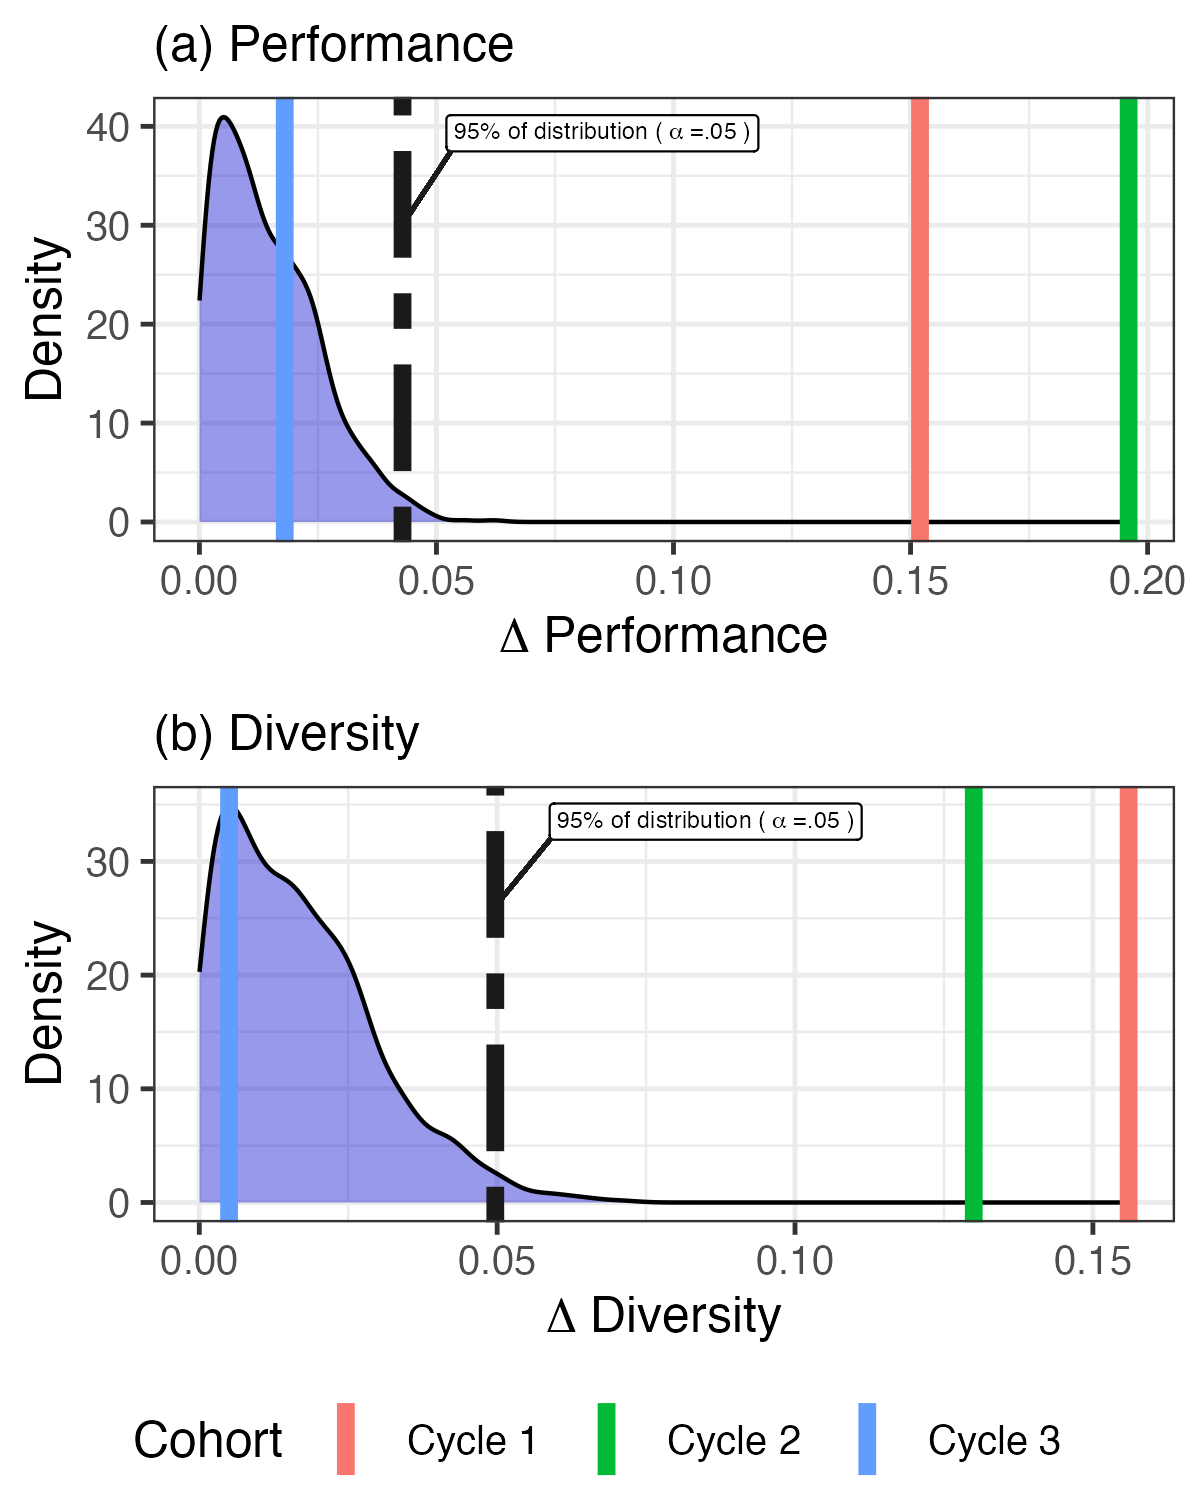
\includegraphics[width=.9\textwidth,height=\textheight,keepaspectratio]{spf/permutation_tests.png} 
    \end{figure}
    
    \newpage
    \begin{figure}[!htb]
    \centering
        \caption{This figure plots the percentile of average expert-judged project quality (i.e. performance) by deciles of cognitive, peer, and traditional scores for the Cycle 2021 cohort. The cognitive score is the percentile of the candidate's IQ, the peer score is the percentile of the average peer assessment of each applicant video, and the traditional score is the average percentile of a candidate's IQ and project essay rating.   } \label{fig:alt_talent_dist}
      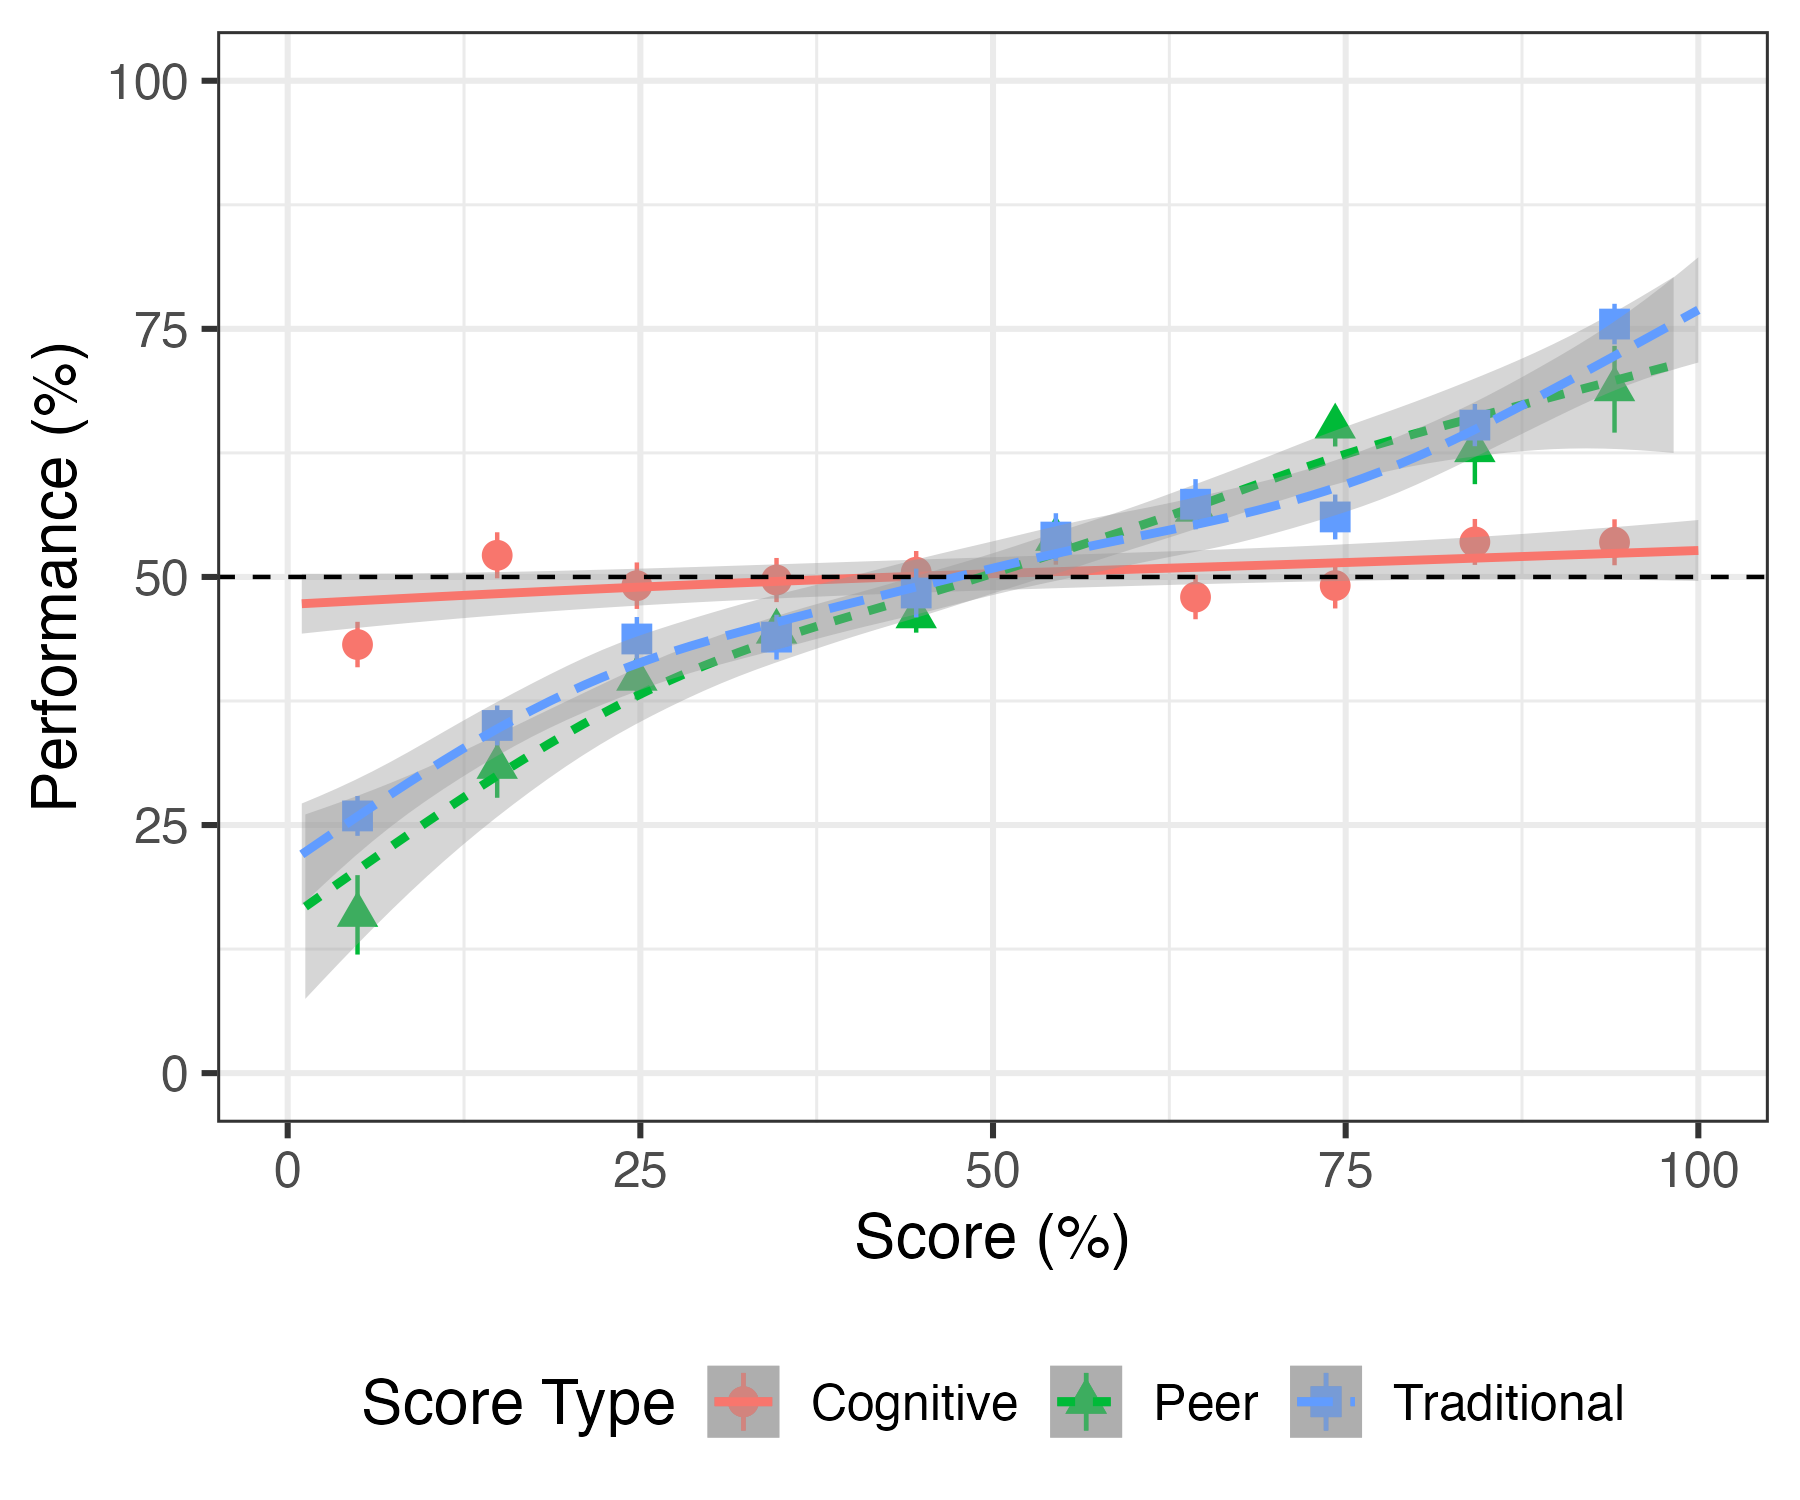
\includegraphics[width=\textwidth,height=\textheight,keepaspectratio]{spf/pq_by_scores_c1.png} 
    \end{figure}
    
    \newpage
    \begin{figure}[!htb]
    \centering
        \caption{This figure plots the average of various measures of applicant socioeconomic (dis)advantage by deciles of cognitive, peer, and traditional scores for the cycle 1 cohort. The measures of (dis)advantage from Panel A to D in order are predicted mean parent income (yearly), years of education of most educated parent, whether or not the applicant lives in a globally poor household (mean parent income less than \$1,000 a year), and whether or not the applicant lives in a poor country (less than \$12,000 GDP per capita). The cognitive score is the percentile of the candidate's IQ, the peer score is the percentile of the average peer assessment of each applicant video, and the traditional score is the average percentile of a candidate's IQ and project essay rating.  } \label{fig:disadvantage_corr}
      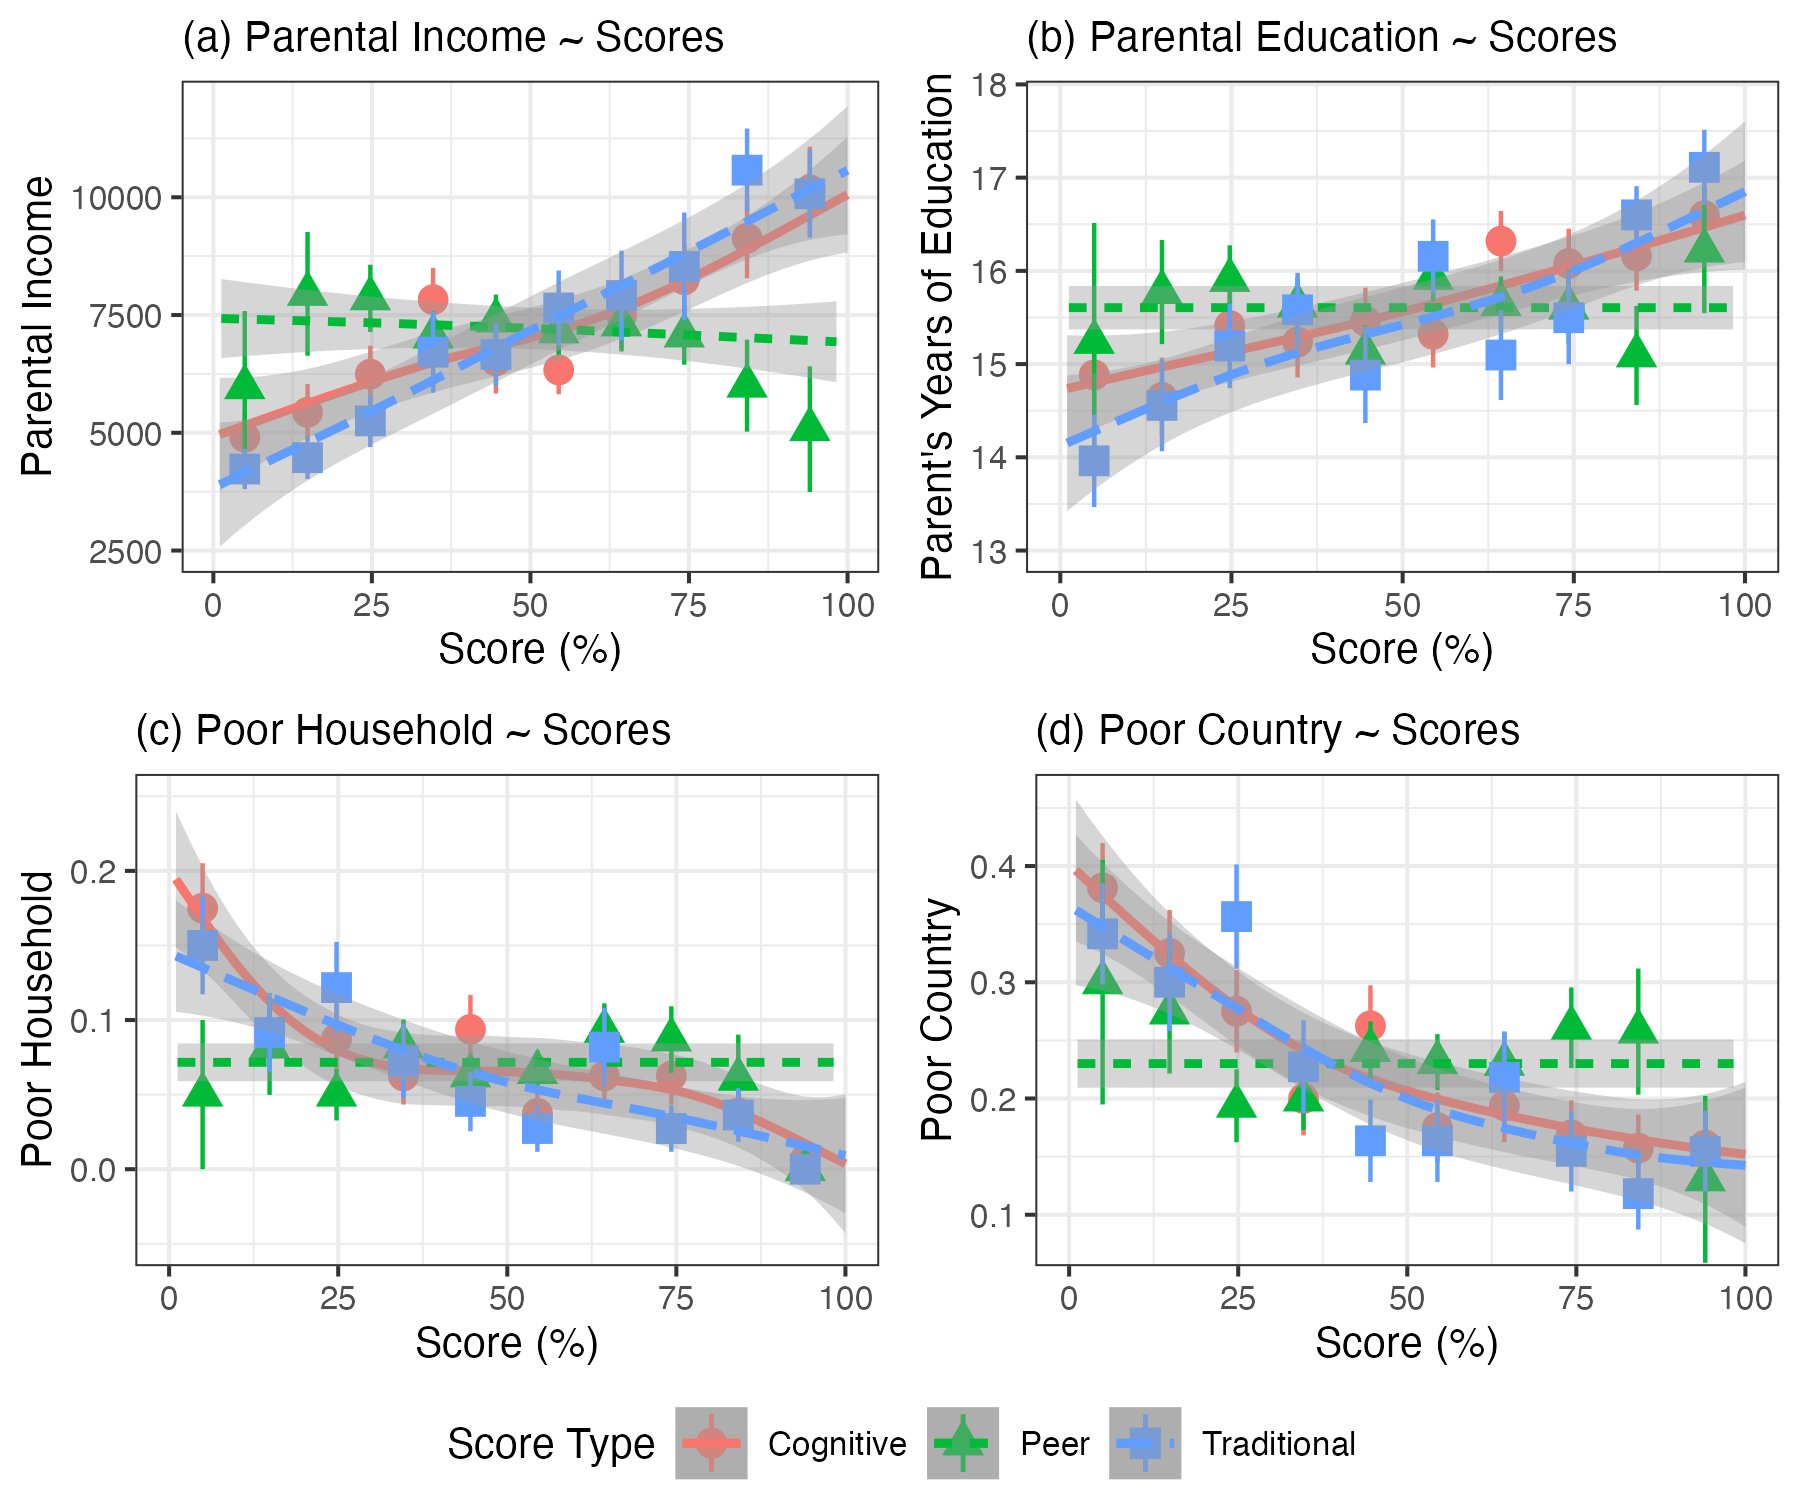
\includegraphics[width=\textwidth,height=\textheight,keepaspectratio]{spf/disadvantage_by_scores.png} 
    \end{figure}
    
    \newpage
    \begin{figure}[!htb]
    \centering
        \caption{This figure displays various SPF estimates for the  finalist cohort using the program's notion of diversity (Panel a), a disadvantage notion of diversity (Panel b), and a representativeness notion of diversity (Panel c). The y-axes represent diversity scores while the x-axes represent average cohort performance (i.e. project scores). The green curves are our estimates of three alternative cycle 1 SPFs, which are estimates the upper bound of diversity that is achievable at every level of cohort performance. Each dot represents the performance and diversity of cohorts had they been selected using those with the highest cognitive (blue), traditional (green), or peer (red) scores.  Each dot represents the performance and diversity of cohorts had they been selected using only cognitive ability (blue), a combination of written essay judgements and cognitive ability (aka a "traditional" score, which is green), and just peer review (red).} \label{fig:alt_screen}
      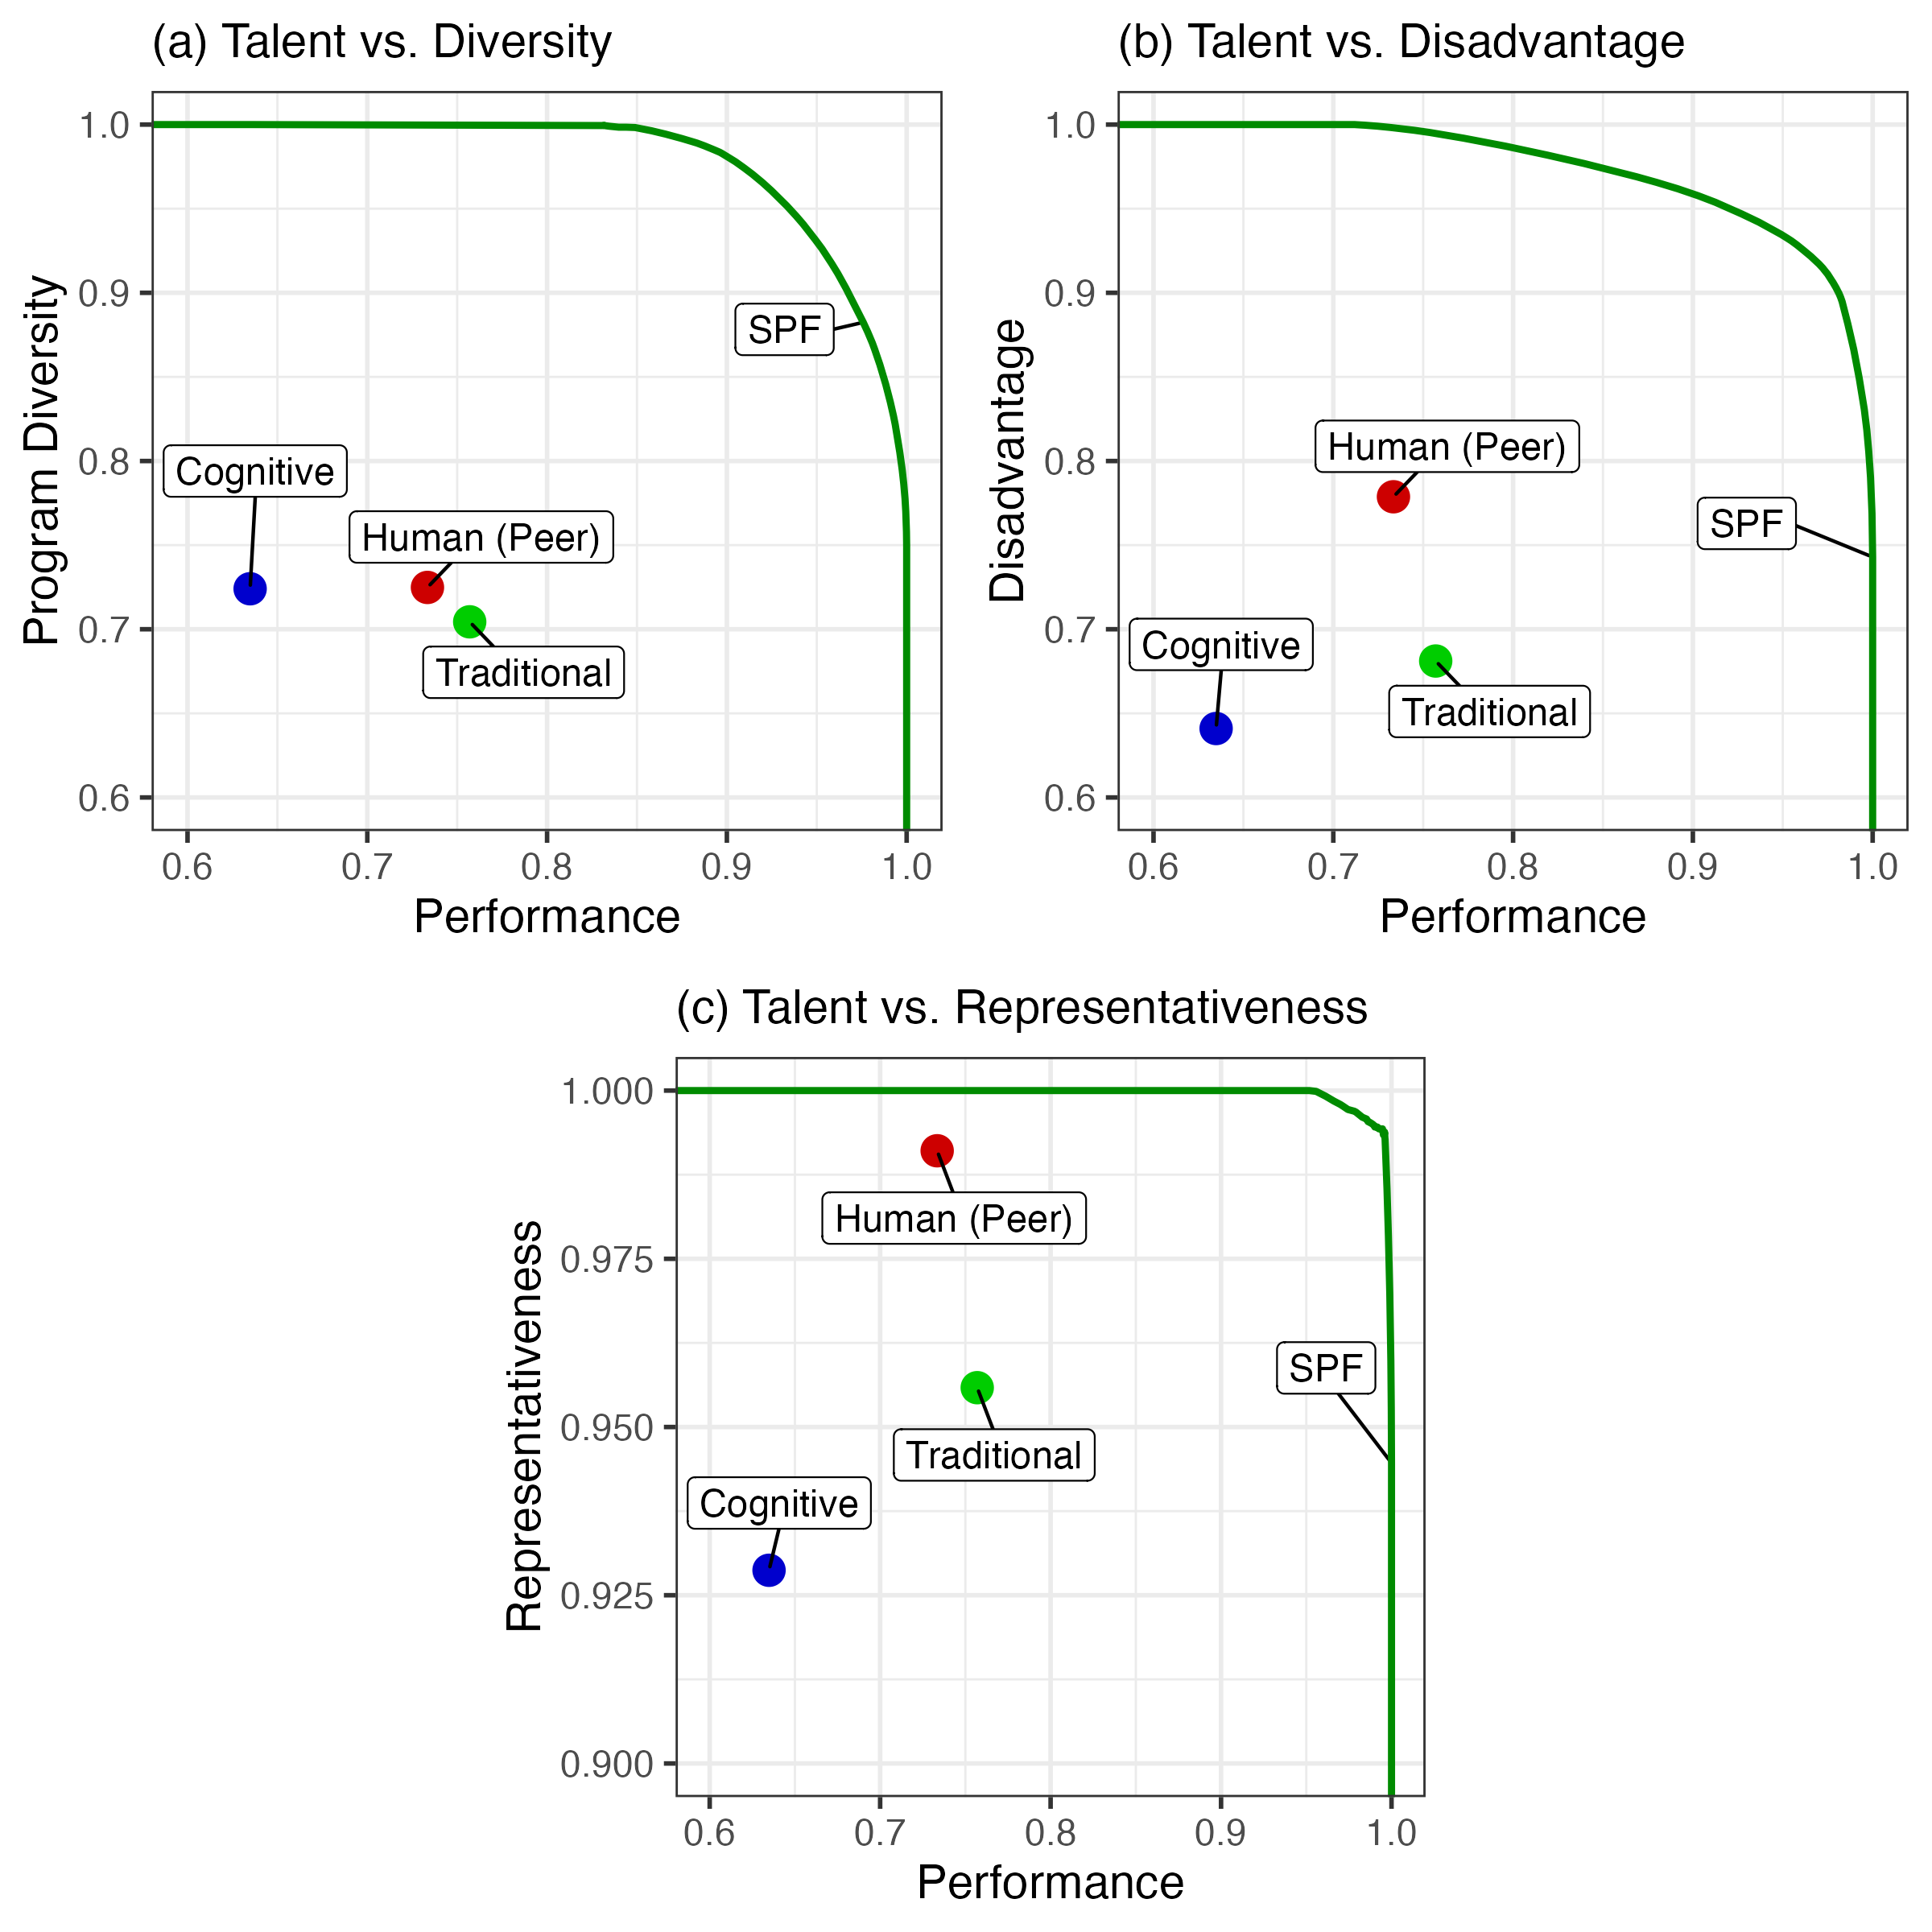
\includegraphics[width=\textwidth,height=\textheight,keepaspectratio]{spf/alt_screening_performance.png} 
    \end{figure}
    
    \newpage
    \begin{figure}[!htb]
    \centering
        \caption{This figure displays the SPF we estimated for the cycle 1 finalist cohort and an SPF based on a more traditional method of measuring performance (i.e. the average of cognitive ability and an essay assessment). The y-axis represents the diversity score while the x-axis represents average cohort performance on projects or the traditional score. The vertical distance between the SPFs represents the difference in maximal diversity conditional on a cohort performing at a particular percentile of both scores. } \label{fig:compare_div_tradeoffs}
      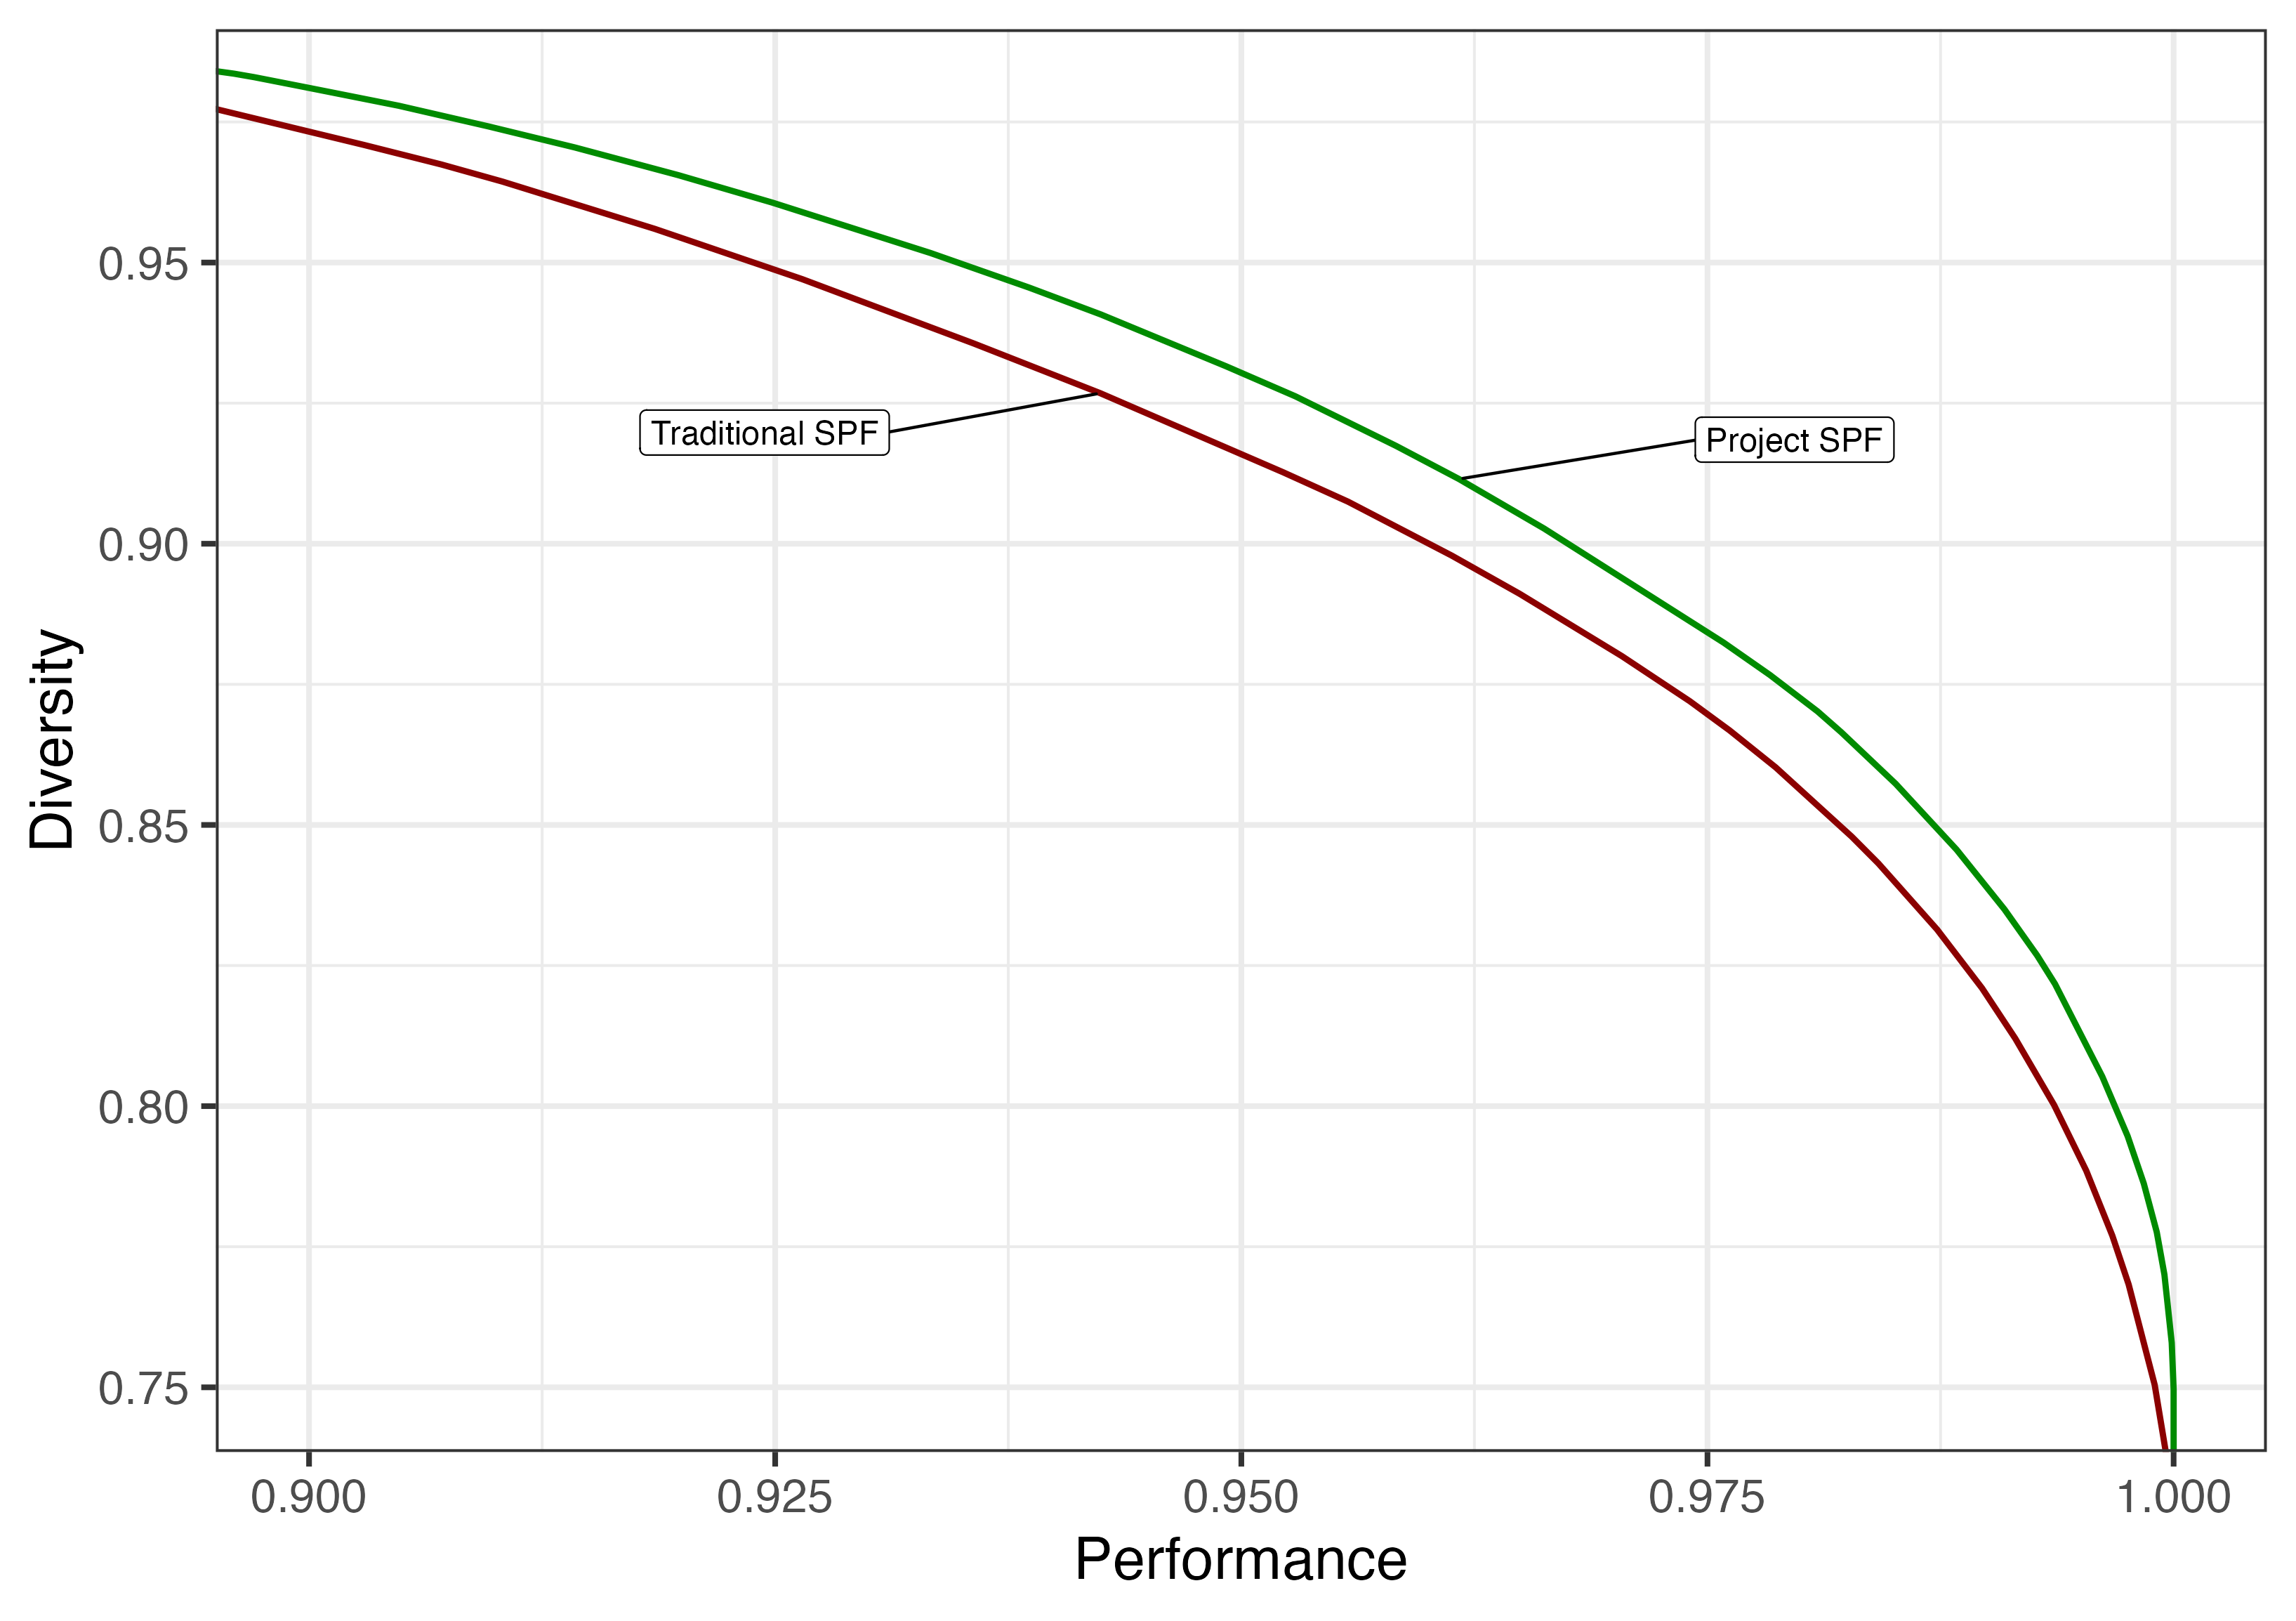
\includegraphics[width=\textwidth,height=\textheight,keepaspectratio]{spf/alt_merit_spfs.png} 
    \end{figure}
    
    \newpage
    
\begin{table}[htbp] 
    \centering 
    \caption{Summary Statistics:  Program Applicants. Raw data come from surveys completed by applicants. Data are pooled across three application years.}
    \label{tab:pooled_demo}
    \begin{tabular}{@{\extracolsep{5pt}}lccccc} 
    \\[-1.8ex]\hline 
    \hline \\[-1.8ex] 
    \emph{Panel A: Demographics} & \multicolumn{1}{c}{N} & \multicolumn{1}{c}{Mean} & \multicolumn{1}{c}{St. Dev.} & \multicolumn{1}{c}{Min} & \multicolumn{1}{c}{Max} \\ 
    \hline \\[-1.8ex] 
    Male & 5,772 & 0.41 & 0.49 & 0 & 1 \\ 
    Age & 5,770 & 16.43 & 0.81 & 15 & 18 \\ 
    Poor Country & 5,720 & 0.42 & 0.49 & 0 & 1 \\ 
    Poor Household & 5,772 & 0.18 & 0.38 & 0 & 1 \\ 
    Yrs of Parent Education & 5,772 & 15.21 & 4.45 & 0 & 20 \\ 
    Mean Parent Income (\$) & 5,772 & 18,891 & 39,617 & 227 & 250,000 \\ 
    \hline
    & & & & & \\
    \emph{Panel B: Global Region} & \multicolumn{1}{c}{N} & \multicolumn{1}{c}{Mean} & \multicolumn{1}{c}{St. Dev.} & \multicolumn{1}{c}{Min} & \multicolumn{1}{c}{Max} \\ 
    \hline
    Latin America & 5,770 & 0.25 & 0.43 & 0 & 1 \\ 
    Sub-Saharan Africa & 5,770 & 0.20 & 0.40 & 0 & 1 \\ 
    Middle East & 5,770 & 0.18 & 0.38 & 0 & 1 \\ 
    Canada/US/UK+ & 5,770 & 0.14 & 0.35 & 0 & 1 \\ 
    India & 5,770 & 0.08 & 0.27 & 0 & 1 \\ 
    East Asia & 5,770 & 0.06 & 0.23 & 0 & 1 \\ 
    Western Europe & 5,770 & 0.04 & 0.20 & 0 & 1 \\ 
    Eastern Europe & 5,770 & 0.04 & 0.20 & 0 & 1 \\ 
    Caribbean/Pacific Islands & 5,770 & 0.01 & 0.08 & 0 & 1 \\ 
    \hline \hline \\[-1.8ex] 
    \end{tabular} 
    \end{table} 
    
    \newpage
    \begin{table}[!htbp] \centering 
      \caption{Summary Statistics: Project Reviewers. Raw data come from surveys completed by applicants. Data are pooled across three application years.}\label{tab:pooled_rev_demo}
      \label{} 
    \begin{tabular}{@{\extracolsep{5pt}}lccccc} 
    \\[-1.8ex]\hline 
    \hline \\[-1.8ex] 
    \emph{Panel A: Demographics} & \multicolumn{1}{c}{N} & \multicolumn{1}{c}{Mean} & \multicolumn{1}{c}{St. Dev.} & \multicolumn{1}{c}{Min} & \multicolumn{1}{c}{Max} \\ 
    \hline \\[-1.8ex] 
    Male & 1,290 & 0.43 & 0.50 & 0 & 1 \\ 
    Age & 1,309 & 44.50 & 19.99 & 19 & 75 \\ 
    Poor Country & 1,321 & 0.46 & 0.50 & 0 & 1 \\ 
    \hline
    & & & & & \\
    \emph{Panel B: Global Region} & \multicolumn{1}{c}{N} & \multicolumn{1}{c}{Mean} & \multicolumn{1}{c}{St. Dev.} & \multicolumn{1}{c}{Min} & \multicolumn{1}{c}{Max} \\ 
    \hline
    Canada/US/UK+ & 1,334 & 0.37 & 0.48 & 0 & 1 \\ 
    India & 1,334 & 0.28 & 0.45 & 0 & 1 \\ 
    Western Europe & 1,334 & 0.07 & 0.25 & 0 & 1 \\ 
    Middle East & 1,334 & 0.07 & 0.26 & 0 & 1 \\ 
    Sub-Saharan Africa & 1,334 & 0.06 & 0.24 & 0 & 1 \\ 
    Latin America & 1,334 & 0.06 & 0.24 & 0 & 1 \\ 
    East Asia & 1,334 & 0.06 & 0.24 & 0 & 1 \\ 
    Eastern Europe & 1,334 & 0.01 & 0.12 & 0 & 1 \\ 
    Caribbean/Pacific Islands & 1,334 & 0.004 & 0.07 & 0 & 1 \\ 
    \hline \hline \\[-1.8ex] 
    \end{tabular} 
    \end{table} 
% \begin{savequote}[8cm]
% Alles Gescheite ist schon gedacht worden.\\
% Man muss nur versuchen, es noch einmal zu denken.

% All intelligent thoughts have already been thought;\\
% what is necessary is only to try to think them again.
%   \qauthor{--- Johann Wolfgang von Goethe \cite{von_goethe_wilhelm_1829}}
% \end{savequote}

\chapter{\label{ch:discussion}Discussion}

\minitoc

\section{Selection-Oriented AI}
In this thesis, we explore the role of AI systems as Decision Support Tools (DSTs) in talent identification. We find that existing AI systems often fail to meet the needs of selection practitioners, particularly for in-process decision-making. In response, we propose a new paradigm, Selection-Oriented AI (SOAI). While present human-centric paradigms see stakeholders as the centres of design efforts, the problem of selecting talent doesn't lend itself to this framing. In addition to the selection organisation, interested in selecting the best cohort they can, and the applicants, interested in being selected, society at large has interest in the outcomes of selection processes. In particular, social values such as fairness, diversity, integrity, justice, etc. should be upheld. In building tools with selection practitioners as the centre of design, we risk neglecting these broader social values. SOAI seeks to address this by centering the design of AI systems around the social values that selection processes should uphold; while this involves designing around the people making selection decisions, it does not end with their satisfaction. Rather, it requires evaluations of the social impact of selection processes and the tools that support them.

\section{Design Recommendations for SOAI Designers}
\subsection{Design for Specific Social Values}
While we wish to design to support all social values in the selection process, Chapter \ref{ch:diversity} demonstrates the difficulty of unpacking the social value of diversity, and we find success instead focusing on smaller component values that comprise diversity. We suggest this generalises to SOAI practices in general. Rather than designing around myriad values, only to find conflicting design implications of these disparate values, designers seeking to support social values in selection processes should focus on specific social values worthy of consideration.

\subsection{Identify Decision Points with the Decision Matrix}
In Chapter \ref{ch:context}, we conceive of selection as a series of decisions. We introduce the Decision Matrix framework to categorise the many decision points that selection practitioners face according to their two most germane axes: the stakes of the decision and its stage in selection. This framework allows designers to evaluate the suitability of AI systems as DSTs for groups of related decision points by determining desired properties for quadrants of the Decision Matrix, then designing for and evaluating those properties. We recommend that designers use the Decision Matrix to identify the decision points relevant to their context and evaluate the suitability of AI systems as DSTs for those points, but to be cautious, as the Decision Matrix framework provides a necessary, but perhaps not sufficient, set of properties. 

\subsection{Balance Quantitative and Qualitative Information in Presentation}
Human decision-makers often desire both a qualitative understanding of applicants and quantitative metrics to compare them. In Chapters \ref{ch:xai} and \ref{ch:diversity}, we find that selection practitioners from programs A and B seek to make decisions informed by both kinds of information; despite this, the desired balance between these modes of information varies based both on practitioner and type of decision. When quantitative information is neglected, practitioners are forced to make decisions on a case-by-case basis without important numerical context comparing applicants to a larger group; when qualitative information is neglected, practitioners are unable to consider applicants holistically. Developers following SOAI should consider the balance between quantitative and qualitative information in their systems, and design their systems to provide both when necessary.

\subsection{Evaluate Real Change in Addition to Subjective Satisfaction}
\textcite{Lipton} critiques explainable AI (xAI) systems on the grounds that they risk satisfying the subjective desires of the users while failing to improve objective outcomes. In Chapter \ref{ch:xai}, we confirm that this critique applies to some post-hoc justifications of model recommendations, as the justifications were found to yield an unwarranted increase in trust in the human decision-makers. Thus, it is important to define and evaluate measures of the social values that DSTs intend to support; when evaluating these DSTs, they should not be evaluated human-centrically (i.e., according to their users' satisfaction), but should instead be evaluated on whether their employment improves social outcomes.

\section{Limitations and Future Work}
While quantitative analyses were performed on a variety of participants from program applicants to Prolific members, our qualitative analyses were limited to a small number of selection practitioners from only two programs. While these programs are leaders in the global talent selection context, findings applied to these two programs may not apply directly to other programs. Additionally, while SOAI is likely applicable to related selection contexts such as university selection or job hiring, further research is needed to explore the limits of its generalisability.

We deliberately do not engage applicants in our process. In general, \textcite{Boaz_Hanney_Borst_O’Shea_Kok_2018} contend that human-centred design should consider the positions of all stakeholders. More specifically, \textcite{venn-wycherley_realities_2024} argue that human-centred research in a classroom setting should consider both educators and students. Unlike other scenarios, though, applicant and selection practitioner organisation incentives conflict; and while most HCI contexts would see a need to balance these groups' needs in designing for the space, we conclude that the social aims of the selection problem itself supersede both groups. As selection practitioners most often find themselves aligned to these social aims, we focus on them. Future work should seek to engage applicants in this context. That said, work exploring the perspectives of applicants should consider first the value and ultimate aim of selection.

Much of our work depends on the contested assumption that global selection processes further societal interests, and that thus supporting the selection process improves social outcomes. \textcite{Warikoo_2019} critiques diversity in elite institutions on the grounds that it merely serves to maintain the status quo. We have contended in Chapter \ref{ch:diversity} that, due to the global talent search's broad reach and engagement with people from a truly diverse set of backgrounds, this critique does not apply here. If it does apply here, the implications for SOAI would be dire. Future work should explore the relationship between selection processes and social outcomes, particularly in the context of diversity.

\section{Conclusion}
In this thesis, we pioneer a new paradigm of AI design for selection processes, Selection-Oriented AI (SOAI). Chapters \ref{ch:xai} and \ref{ch:genai} find that existing AI systems often fail to meet the needs of selection practitioners, particularly for in-process decision-making. In response, we propose a new paradigm, SOAI, which seeks to centre the design of AI DSTs not around the selection practitioners but around the social aims of selection they seek to practice. Chapters \ref{ch:diversity} and \ref{ch:spf} apply SOAI principles to design DSTs to support considerations of diversity in selection; we implement a prototype designed to satisfy selection practitioner desires and find that it improves both diversity and performance outcomes in selection. We then provide a set of design recommendations for SOAI designers, including focusing on specific social values, identifying decision points with the Decision Matrix, balancing quantitative and qualitative information, and evaluating real change in addition to subjective satisfaction. We conclude with a call for more selection-oriented work, applying data-driven support to this difficult and sensitive problem.

%%%%% APPENDICES
% Starts lettered appendices, adds a heading in table of contents, and adds a
%    page that just says "Appendices" to signal the end of your main text.
\startappendices
% Add or remove any appendices you'd like here:
% \begin{savequote}[8cm]
% \textlatin{Cor animalium, fundamentum e\longs t vitæ, princeps omnium, Microco\longs mi Sol, a quo omnis vegetatio dependet, vigor omnis \& robur emanat.}

% The heart of animals is the foundation of their life, the sovereign of everything within them, the sun of their microcosm, that upon which all growth depends, from which all power proceeds.
%   \qauthor{--- William Harvey \cite{harvey_exercitatio_1628}}
% \end{savequote}

\chapter{\label{app:protocolmockup}Study Protocols}

\minitoc

\section{Chapter \ref{ch:xai} Design Workshops}\label{app:xaiprotocol}
We split our N=8 participants into two groups of 4 (G1 and G2) to run two participatory design workshops. As these are group discussions, actual programming deviates from the protocol slightly.

Our research question for both workshops is: ``Are SHAP explanations useful?''; however, to frame each workshop, we told both groups that we were interested in the answer to two questions: ``What does this technology tell us about the algorithm’s scores?'' and ``How do we envision this technology being used in future selection processes?''.

Following this, we gave both groups a 15-minute demonstration of the technology, where we described a sample case, gave some example insights, and answered any questions participants had. 

The main task for our workshops consists of hands-on cases examining a SHAP-based ``waterfall plot'' explanation of a program applicant's score. An example case can be seen in Figure \ref{fig:sample_case}. Each case is presented to participants as a single slide on a presented slideshow, with additional questions asked by the researchers to prompt discussion. We show each group 5 different cases and spend an average of 10 minutes on each case.

For each case, we ask some of the following questions to prompt discussion:

\begin{enumerate}
    \item Why are we viewing this applicant?
    \item What comments are we responding to?
    \item What does the technology appear to say about this candidate?
    \item Does the technology address the comment we are responding to?
    \item What does this case say about the algorithm as a whole?
    \item Does this case necessitate changes to the algorithm?
\end{enumerate}

Finally, after all cases had been examined, we moved to a short reflection on the technology as a whole. We asked participants to answer:

\begin{enumerate}
    \item What did you think was useful about the technology presented?
    \item What was lacking?
    \item How might this be improved?
\end{enumerate}


\section{Chapter \ref{ch:diversity} Interviews}\label{app:divprotocol1}
For the individual interviews, we follow a semi-structured protocol. Following the methodology of \textcite{braun_using_2006}, we do not limit our analysis to these questions. Instead, we deviate from this script as guided by the conversations and our overarching research questions, then we allow themes to emerge naturally from the data. Our interview research questions (also found in Section \ref{ssec:methods1}) are:

\begin{enumerate}
    \item What is diversity?
    \item Which elements of diversity matter in a selection context? Why?
    \item How could technology assist in operationalising diversity?
\end{enumerate}

We interview 15 individuals from two different talent identification organisations. We conduct each interview separately. We first ask a few questions about the factors that go into decision-making:

\begin{enumerate}
    \item We're going to take a step back and discuss a hypothetical selection scenario for a fellowship for a group of young people. In this scenario, you have full control over who is selected.
    \item Could you please list some things you think are important in deciding who to accept?
    \item (Can skip) Which of (these things) are about the individual applicant's performance?
    \item What are (these remaining things) about? 
    \item (Or:) Why are (these things) important?
\end{enumerate}

We then ask participants to define diversity, to break it down into elements, and to discuss why diversity is important:

\begin{enumerate}
    \item Now I want to talk about diversity. Keeping your list in mind, can you please define diversity?
    \item (If the definition is too short) Could you please elaborate on (pick a part)
    \item Why do we care about this definition of diversity?
    \item Now, if you were going to break your definition into some elements or facets, what would those be?
    \item (If they talk about holistic diversity) What considerations are important when looking at diversity holistically?
    \item (If elements are vague) How does (pick a metric) factor into your understanding of (element)?
    \item Which elements or considerations are most important?
    \item How do we measure these facets of diversity?
    \item (If this measurement isn't concrete) Imagine you had a ``magic metric'' that perfectly measured diversity. What does this metric do?
\end{enumerate}

Next, we run two short exercises from the participatory design literature. The first is called ``crazy 8s'', wherein participants are given 8 minutes to come up with 8 ideas. For these ideas, we ask participants to think about technologies that might help them better understand diversity in selection:

\begin{enumerate}
    \item Now I want to talk about technology we can build to support thinking about tradeoffs around diversity. Remember that we're stepping away from existing processes and solutions.
    \item We're going to start with an exercise called ``crazy 8s''. For the next 8 minutes, we're going to spend one minute each developing a technology that might help us better understand diversity in selection. These technologies don't have to make sense or be possible; I just want you to think of things that might help you think through diversity. This activity is difficult; don't worry if you find yourself struggling or sounding silly.
    \item Take a second to think about a technology. When you're ready, please describe it.
    \item (If the technology is unclear) Could you please elaborate on (unclear part)?
\end{enumerate}

The second is called ``the magic app'', wherein participants are asked to elaborate on a single idea for an application, waving away technical details as `magic':

\begin{enumerate}
    \item Now let's dig deeper into one hypothetical ``magic app'' designed to help us better understand tradeoffs around diversity in selection. The magic app can do anything you might want it to in any way you might want. What does your magic app do?
    \item (If the app has visuals) What do your visuals look like?
    \item (If the app is pure text) What sorts of visualisations might help you?
    \item (If the app has buttons or sliders) What do your buttons do?
    \item (If the app doesn't have any interactivity) How might you interact with this app?
    \item Now we are going to split the app out into different ``pages''
    \item (If they haven't already done this) The individual-level page: each applicant will have their own individual-level page, which will say things about that applicant
    \item (If they haven't already done this) The cohort-level page: each possible cohort will have its own cohort-level page, which will update any time we make changes to the cohort.
    \item (For each page) What happens on this page?
    \item What is the experience of using this page like?
    \item (If the page has visuals) What do your visuals look like?
    \item (If the page is pure text) What sorts of visualisations might help you?
    \item (If the page has buttons or sliders) What do your buttons do?
    \item (If the page doesn't have any interactivity) How might you interact with this app?
    \item (For each different feature of the page) What makes (feature) useful to you?
    \item Thank you! Is there anything else you would like to add?
\end{enumerate}

\section{Chapter \ref{ch:diversity} Design Workshops}\label{app:divprotocol2}
For the participatory design workshops, we split our participants by organisation. As some individuals could not attend the second session, we have one group of 6 and another of 7. As these are much larger group discussions, we deviate further from our protocol.

The task for these workshops consists of hands-on sessions with different technologies. The technologies are designed and mocked up based on the thematic analysis of the interviews. These technologies are presented to participants via Miro, where they are free to interact with and annotate them. Our research questions for this workshop are:

\begin{enumerate}
    \item What prototypes best promote diversity?
    \item What elements of these prototypes facilitate their success?
\end{enumerate}

Or, for each prototype: ``How and why does this prototype promote diversity in talent identification?''. Again, though we write a list of questions targeted at these questions, we do not limit our analysis to these questions \cite{braun_using_2006}. Instead, we deviate from this script as guided by the conversations and our overarching research questions, then we allow themes to emerge naturally from the data \cite{braun_using_2006}. For each technology prototype shown, we have questions:

\begin{enumerate}
    \item This prototype describes... Are any of you familiar with this?
    \item In what follows, we're going to discuss this prototype. Let's start with: is it easy to read for you? What does it say? 
    \item What questions do you have upon seeing this prototype? Feel free to write these down.
    \item How would you use this prototype in a hypothetical selection procedure?
    \item How (else) would this prototype fit into your current selection procedure?
    \item How would your current selection procedure make best use of this prototype? Would the process need to be changed? Do you think this would be beneficial?
\end{enumerate}

Finally, at the end of our workshop, after we have covered all of the prototypes, we ask participants to place a star next to their favourite prototype on the Miro board \cite{Gatian_1994,Griffiths_Johnson_Hartley_2007}.
% \begin{savequote}[8cm]
% \textlatin{Cor animalium, fundamentum e\longs t vitæ, princeps omnium, Microco\longs mi Sol, a quo omnis vegetatio dependet, vigor omnis \& robur emanat.}

% The heart of animals is the foundation of their life, the sovereign of everything within them, the sun of their microcosm, that upon which all growth depends, from which all power proceeds.
%   \qauthor{--- William Harvey \cite{harvey_exercitatio_1628}}
% \end{savequote}

\chapter{\label{app:math}Mathematics and Computation}

\minitoc

\section{ChatGPT Code Generation for Chapter \ref{ch:genai}}

\section{Proofs of Submodularity and Monotonicity for Chapter \ref{ch:spf}}

\begin{theorem} 
    Submodularity is closed under weighted addition. \label{thm:submodularity_additive}
    \end{theorem}
    
    \begin{proof}
    \begin{equation}
        \label{eq:submodularity_additive}
        \begin{split}
            \forall Y \subseteq U, X \subseteq Y, x \in U \setminus Y, a \geq 0, b \geq 0: & F_1(X \cup \{x\}) - F_1(X) \leq F_1(Y \cup \{x\}) - F_1(Y) \\
            &\land F_2(X \cup \{x\}) - F_2(X) \leq F_2(Y \cup \{x\}) - F_2(Y) \\
            \implies & a*F_1(X \cup \{x\}) - a*F_1(X) \leq a*F_1(Y \cup \{x\}) - a*F_1(Y) \\
            &\land b*F_2(X \cup \{x\}) - b*F_2(X) \leq b*F_2(Y \cup \{x\}) - b*F_2(Y) \\
            \implies & a*F_1(X \cup \{x\}) - a*F_1(X) + b*F_2(X \cup \{x\}) - b*F_2(X) \\
            &\leq a*F_1(Y \cup \{x\}) - a*F_1(Y) + b*F_2(Y \cup \{x\}) - b*F_2(Y) \\
            \implies & a*F_1+b*F_2(X \cup \{x\}) - a*F_1+b*F_2(X) \\
            &\leq a*F_1+b*F_2(Y \cup \{x\}) - a*F_1+b*F_2(Y) \\ \nonumber
        \end{split}
    \end{equation}
    \end{proof}
    
    \begin{theorem} 
    Monotonicity is closed under weighted addition. \label{thm:monotonicity_additive}
    \end{theorem}
    \begin{proof}
    \begin{equation}
        \label{eq:mononicity_additive}
        \begin{split}
            \forall Y \subseteq U, X \subseteq Y, a \geq 0, b \geq 0: & F_1(X)\leq F_1(Y) \land F_2(X)\leq F_2(Y) \\
            \implies & a*F_1(X)\leq a*F_1(Y) \land b*F_2(X)\leq b*F_2(Y) \\
            \implies & a*F_1(X) + b*F_2(X) \leq a*F_1(Y) + b*F_2(Y) \\
            \implies & a*F_1+b*F_2(X) \leq a*F_1+b*F_2(Y) \\ \nonumber
        \end{split}
    \end{equation}
    \end{proof}
    
    \begin{theorem} 
    The class of functions $F$ as defined in Equation \ref{eq:f_spec} is submodular and monotone.\label{thm:f_sub_mon}
    \end{theorem}
    \begin{proof}
    By construction, $F$ is the weighted sum of $P$ and $D$. But $D$ is the weighted sum of functions $\delta_g^{prop}$ and $\delta_G^{count}$.
    It is trivial to see that $P$ is submodular and monotone. We have already demonstrated that $\delta_g^{prop}$ and $\delta_G^{count}$ are submodular and monotone. Thus, by Theorems \ref{thm:submodularity_additive} and \ref{thm:monotonicity_additive}, $F$ is submodular and additive.
    \end{proof}
% \begin{savequote}[8cm]
% \textlatin{Cor animalium, fundamentum e\longs t vitæ, princeps omnium, Microco\longs mi Sol, a quo omnis vegetatio dependet, vigor omnis \& robur emanat.}

% The heart of animals is the foundation of their life, the sovereign of everything within them, the sun of their microcosm, that upon which all growth depends, from which all power proceeds.
%   \qauthor{--- William Harvey \cite{harvey_exercitatio_1628}}
% \end{savequote}

\chapter{\label{app:figures}Reference Figures and Tables}

\minitoc

\section{Sample Explanations from Chapter \ref{ch:xai}}\label{app:xaifigures}

\begin{figure}[htbp]
    \centering
    \includegraphics[width=0.9\linewidth]{plots/survey-shap.png}
    \caption{This figure shows sample SHAP explanations in the $salary$ task}
    \label{fig:shapsalaryfull}
\end{figure}

\begin{figure}[hbtp]
    \centering
    \includegraphics[width=0.9\linewidth]{plots/survey-shap-2.png}
    \caption{This figure shows sample SHAP explanations in the $credit$ task}
    \label{fig:shapcreditfull}
\end{figure}

Figures \ref{fig:shapcreditfull} and \ref{fig:shapsalaryfull} show sample SHAP explanations in the $salary$ and $credit$ tasks. In both cases, features can be seen along the y-axis, while feature importance is shown based on direction and magnitude of the associated bar.

\begin{figure}[htbp]
    \centering
    \includegraphics[width=0.8\linewidth]{plots/survey-anchor.png}
    \caption{This figure shows sample Anchor explanations in the $salary$ task}
    \label{fig:anchorsalaryfull}
\end{figure}

\begin{figure}[hbtp]
    \centering
    \includegraphics[width=0.9\linewidth]{plots/survey-anchor-2.png}
    \caption{This figure shows sample Anchor explanations in the $credit$ task}
    \label{fig:anchorcreditfull}
\end{figure}

Figures \ref{fig:anchorcreditfull} and \ref{fig:anchorsalaryfull} shows sample Anchor explanations in $salary$ and $credit$. In both cases, the explanation shows a set of rules that, when jointly followed, increases the likelihood that the model will yield the displayed prediction.

\begin{figure}[htbp]
    \centering
    \includegraphics[width=0.6\linewidth]{plots/survey-confidence.png}
    \caption{This figure shows sample Confidence explanations in the $salary$ task}
    \label{fig:confidencesalaryfull}
\end{figure}

\begin{figure}[hbtp]
    \centering
    \includegraphics[width=0.6\linewidth]{plots/survey-confidence-2.png}
    \caption{This figure shows sample Confidence explanations in the $credit$ task}
    \label{fig:confidencecreditfull}
\end{figure}

Figures \ref{fig:confidencecreditfull} and \ref{fig:confidencesalaryfull} show sample Confidence explanations in the $salary$ and $credit$ tasks. In both cases, the explanation is simply one sentence containing the model's confidence parameter.


\section{Figures and Tables for Chapter \ref{ch:spf}}
\begin{landscape}
    \begin{figure}[!htb]
    \centering
        \caption{Distribution of Cycle 1 Applicant Countries (Top 5 Labeled) }\label{fig:dist_countryies_c1}
      \includegraphics[width=1.3\textwidth,height=\textheight,keepaspectratio]{results/figures/candidate_countries_yr1.png} 
        \begin{notes}
        Data come from surveys completed by applicants. Data are solely from the cycle 1 application cohort. Overall applicants come from 105 different countries. The distribution of proportions of applicants by country in this figure are limited to the 50 countries from which there were the most applicants. The top 5 countries are labeled on the figure. 
        \end{notes}
    \end{figure}
    \end{landscape}
    
    \newpage
    \begin{figure}[!htb]
    \centering
        \caption{Using SPFs to Compare Achievable Diversity Across Cohorts}\label{fig:diversity_across_cohorts}
      \includegraphics[width=\textwidth,height=\textheight,keepaspectratio]{results/figures/spf_cohort_comparisons.png} 
        \begin{notes}
        This figure displays the SPFs we estimate for three finalist cohorts. The y-axis represents the diversity score while the x-axis represents average cohort performance (i.e. percentiles of mean project scores). The diversity target is held constant across cohorts, so differences in SPFs conditional on performance represent differences in the capacity to reach the same diversity target at a given level of performance. 
        \end{notes}
    \end{figure}
    
    \newpage
    \newpage
    \begin{figure}[!htb]
        \centering
        \caption{Expert Review Screens}
        \begin{subfigure}[]{\textwidth}
            \centering
                    \caption{Project Essay Review Screen} \label{subfig:essay}
            \includegraphics[width=\linewidth]{results/figures/essay_review_screen.png} 
        \end{subfigure}
        \hline
        \hfill
        \vspace{1em}
        \begin{subfigure}[]{\textwidth}
            \centering
                    \caption{Final Project Review Screen} \label{subfig:project}
            \includegraphics[width=\linewidth]{results/figures/project_review_screen.png} 
        \end{subfigure}
        \hline
        \begin{notes}
        This figure shows example screens that expert reviewers saw when rating essays (Panel \ref{subfig:essay}) and project presentations (Panel \ref{subfig:project}). Both were rated on 15 point scales judging effectiveness and impressiveness of the project. Text of the example project essay and the face of the applicant have both been blurred to protect the identity of the applicants. 
        \end{notes}
    \end{figure}
    
    
    \newpage
    \begin{landscape}
    \null
    \vfill
    \begin{figure}[!htb]
    \centering
        \caption{ICAR Sample Items}\label{fig:icar_items}
    \includegraphics[width=1.3\textwidth,height=\textheight,keepaspectratio]{results/figures/icar_items.png} 
        \begin{notes}
    This figure shows sample items for all three types of questions the program used from International Cognitive Ability Resource (ICAR) assessment. All three item types are best described using language from the \hyperlink{https://icar-project.org/types/index.html}{ICAR website}: the Cube Rotation items "present participants with cube renderings and ask participants to identify which of the response choices is a possible rotation of the target stimuli", the Number Sequence items ask participants to " fill in one or two numbers that follow in the sequence", and the Matrix Reasoning items "contain stimuli that are... 3x3 arrays of geometric shapes with one of the nine shapes missing" (similar to those used in Raven's Progressive Matrices) and participants "are instructed to identify which of six geometric shapes presented as response choices will best complete the stimuli". Because the applicant pool was international, these specific item types were chosen because they rely minimally on knowledge of english. In the program's implementation, each applicant saw 5 questions of each type.
        \end{notes}
    \end{figure}
    \vfill
    \end{landscape}
    
    \newpage
    \null
    \vfill
    \begin{figure}[!htb]
    \centering
        \caption{Instance of Gamified Skills Test}\label{fig:roomworld_instance}
    \includegraphics[width=.6\textwidth,height=\textheight,keepaspectratio]{results/figures/roomworld_instance.png} 
        \begin{notes}
    The gamified skills test applied to applicants in cohort 3 is a game called Roomworld, and a sample level of the game is depicted above. In each level, applicants are challenged to move through the grid using the arrow keys to get the yellow icon to the gift. Shapes within the grid serve as different obstacles and mechanisms for navigating the level. How each obstacle and mechanism work are not explained to the player, as part of the test is about discovering \emph{how} they work. Multidimensional data from the game are collected and aggregated to give players a percentile score. The specific scoring alorithm was developed by researchers in the \hyperlink{https://humaninformationprocessing.com/people/}{Human Information Processing Lab} at Oxford university and has not been provided to us. 
        \end{notes}
    \end{figure}
    \vfill
    
    \newpage
    \begin{figure}[!htb]
    \centering
        \caption{Association of Project Reviews with School Rank} \label{fig:proj_robust_1}
    \includegraphics[width=.9\textwidth,height=\textheight,keepaspectratio]{results/figures/validation_raw.png} 
        \begin{notes}  
        This figure depicts various binscatter plots that reveal the association between college rank and expert-judged project performance. Data used for these plots come from two sources: (1) 121 respondents to a follow-up survey administered to cycle 1 and cycle 2 program applicants and (2) 359 respondents to a survey administered to cohort cycle 2 finalists. In the former, school rank comes from the respondents' self-reported college at which they have matriculated. But, in the latter, school rank is based on the schools that respondents are most interested in attending (i.e. the college they aspire to attend). Panel A depicts the relationship between expert project reviews and school rank pooling together both samples. Panel B plots the relationship conditional on data source. Panel C is limited just to the follow-up survey. Panel D is limited just to the cohort cycle 2 finalists. In the top right of each panel is the coefficient of interest from regressions that correspond to each panel. \\
        
       *** significant at the 1\% level; ** significant at the 5\% level; * significant at the 10\% level
        \end{notes}
    \end{figure}
    
    \newpage
    \begin{figure}[!htb]
    \centering
        \caption{Association of Project Reviews with School Rank (with SES Controls)} \label{fig:proj_robust_2}
    \includegraphics[width=.9\textwidth,height=\textheight,keepaspectratio]{results/figures/validation_w_controls.png} 
        \begin{notes}  
        This figure depicts various binscatter plots that reveal the conditional association between college rank and expert-judged project performance. Data used for these plots come from two sources: (1) 121 respondents to a follow-up survey administered to cycle 1 and cycle 2 program applicants and (2) 359 respondents to a survey administered to cycle 2 finalists. In the former, school rank comes from the respondents' self-reported college at which they have matriculated. But, in the latter, school rank is based on the schools that respondents are most interested in attending (i.e. the college they aspire to attend). Each association depicted is conditional on "SES Controls", which consist of fixed effects for gender, parental education, living in a poor country, and being in a poor household. Panel A depicts the association between school rank and residuals from a regression of expert project reviews on SES Controls in a sample the pools responses from both data sources. Panel B plots the same association, adding a data source fixed effect. Panel C limits just to the follow-up survey. Panel D is limits just to the cohort cycle 2 finalists. In the top right of each panel is the coefficient of interest from corresponding regressions. \\
        
       *** significant at the 1\% level; ** significant at the 5\% level; * significant at the 10\% level
        \end{notes}
    \end{figure}
    
    \newpage
    \begin{figure}[!htb]
        \centering
        \caption{Peer Scores and "Surprisingly" Talented Applicants}\label{fig:peer_ditr}
        \begin{subfigure}[t]{.45\textwidth}
            \centering
                    \caption{Traditional vs. Project Performance} \label{subfig:trad_perf}
            \includegraphics[width=\linewidth]{results/figures/traditional_performance_cor.png} 
        \end{subfigure}
        \hfill
        \vspace{1em}
        \begin{subfigure}[t]{.45\textwidth}
            \centering
                    \caption{Peer vs. Project Performance} \label{subfig:peer_perf}
            \includegraphics[width=\linewidth]{results/figures/peer_performance_cor.png} 
        \end{subfigure}
        \hfill
        \vspace{1em}
        \begin{subfigure}[t]{.45\textwidth}
            \centering
                   \caption{Peer vs. Traditional} \label{subfig:peer_trad}
            \includegraphics[width=\linewidth]{results/figures/peer_traditional_cor.png} 
        \end{subfigure}
            \hfill
        \vspace{1em}
         \begin{subfigure}[t]{.45\textwidth}
            \centering
                   \caption{Peer vs. Project - Traditional} \label{subfig:peer_surp}
            \includegraphics[width=\linewidth]{results/figures/peer_surprise_cor.png} 
        \end{subfigure}
                \hfill
        \vspace{1em}
        \begin{notes}
        Each panel in this figure depicts a binscatter intended to visualize the correlation between two potential screening scores (traditional and peer scores) and expert project performance scores. Panel \ref{subfig:trad_perf} depicts the relationship between the traditional score and project performance. Panel \ref{subfig:peer_perf} depicts the relationship between the peer score and project performance. Panel \ref{subfig:peer_trad} depicts the relationship between the peer score and the traditional score. 
        \end{notes}
    \end{figure}
    
    \newpage
    \begin{figure}[!htb]
    \centering
        \caption{Project Quality by Deciles of Alternative Screening Scores} \label{fig:alt_talent_dist_full}
      \includegraphics[width=\textwidth,height=\textheight,keepaspectratio]{\figurepath/pq_by_scores.png} 
        \begin{notes}
        This figure plots the percentile of average expert-judged project quality (i.e. performance) by deciles of cognitive, peer, and traditional scores for all three cohorts. The cognitive score is the percentile of the candidate's IQ, the peer score is the percentile of the average peer assessment of each applicant video, and the traditional score is the average percentile of a candidate's IQ and project essay rating.   
        \end{notes}
    \end{figure}
    
    \newpage
    \begin{figure}[!htb]
    \centering
        \caption{Socioeconomic (Dis)Advantage by Deciles of Alternative Screening Scores} \label{fig:disadvantage_corr_full}
      \includegraphics[width=\textwidth,height=\textheight,keepaspectratio]{results/figures/disadvantage_by_scores_full.png} 
        \begin{notes}
        This figure plots the average of various measures of applicant socioeconomic (dis)advantage by deciles of cognitive, peer, and traditional scores for all three cohorts. The measures of (dis)advantage from Panel A to D in order are predicted mean parent income (yearly), years of education of most educated parent, whether or not the applicant lives in a globally poor household (mean parent income less than \$1,000 a year), and whether or not the applicant lives in a poor country (less than \$12,000 GDP per capita). The cognitive score is the percentile of the candidate's IQ, the peer score is the percentile of the average peer assessment of each applicant video, and the traditional score is the average percentile of a candidate's IQ and project essay rating.   
        \end{notes}
    \end{figure}
    
    \newpage
    \begin{figure}[!htb]
    \centering
        \caption{Proportion Female by Deciles of Alternative Screening Scores} \label{fig:alt_female_cor}
      \includegraphics[width=.9\textwidth,height=\textheight,keepaspectratio]{results/figures/female_by_scores.png} 
        \begin{notes}
        This figure plots the average proportion female by deciles of cognitive, peer, and traditional scores for the cycle 1 cohort (Panel A) and all cohorts pooled together (Panel B). The cognitive score is the percentile of the candidate's IQ, the peer score is the percentile of the average peer assessment of each applicant video, and the traditional score is the average percentile of a candidate's IQ and project essay rating.   
        \end{notes}
    \end{figure}
    
    
    \newpage
    
    \begin{table}[!htbp]
        \centering
        \caption{Summary Statistics: Program Applicants (Cycle 1). Raw data come from surveys completed by applicants. Data are pooled across all three application years. }
        \label{tab:c1_demo}
    \begin{tabular}{@{\extracolsep{5pt}}lccccc} 
    \\[-1.8ex]\hline 
    \hline \\[-1.8ex] 
    \emph{Panel A: Demographics} & \multicolumn{1}{c}{N} & \multicolumn{1}{c}{Mean} & \multicolumn{1}{c}{St. Dev.} & \multicolumn{1}{c}{Min} & \multicolumn{1}{c}{Max} \\ 
    \hline \\[-1.8ex] 
    Male & 1,591 & 0.33 & 0.47 & 0 & 1 \\ 
    Age & 1,589 & 16.81 & 0.81 & 15 & 18 \\ 
    Poor Country & 1,591 & 0.23 & 0.42 & 0 & 1 \\ 
    Poor Household & 1,591 & 0.07 & 0.26 & 0 & 1 \\ 
    Yrs of Parent Education & 1,591 & 15.61 & 4.73 & 0 & 20 \\ 
    Mean Parent Income (\$) & 1,591 & 7,209 & 8,847 & 356 & 65,174 \\ 
    \hline
    & & & & & \\
    \emph{Panel B: Global Region} & \multicolumn{1}{c}{N} & \multicolumn{1}{c}{Mean} & \multicolumn{1}{c}{St. Dev.} & \multicolumn{1}{c}{Min} & \multicolumn{1}{c}{Max} \\ 
    \hline
    Latin America & 1,591 & 0.46 & 0.50 & 0 & 1 \\ 
    Canada/US/UK+ & 1,591 & 0.15 & 0.36 & 0 & 1 \\ 
    Middle East & 1,591 & 0.11 & 0.32 & 0 & 1 \\ 
    Sub-Saharan Africa & 1,591 & 0.09 & 0.29 & 0 & 1 \\ 
    India & 1,591 & 0.06 & 0.23 & 0 & 1 \\ 
    Western Europe & 1,591 & 0.05 & 0.22 & 0 & 1 \\ 
    East Asia & 1,591 & 0.04 & 0.19 & 0 & 1 \\ 
    Caribbean/Pacific Islands & 1,591 & 0.003 & 0.05 & 0 & 1 \\ 
    Eastern Europe & 1,591 & 0.00 & 0.00 & 0 & 0 \\ 
    \hline \hline \\[-1.8ex] 
    \end{tabular} 
    \end{table} 
    
    \begin{landscape}
    \null
    \hfill
    \begin{table}[!htb]
    \caption{Key Measures and Components. This table provides an overview of the key measures used in this paper. Column 1 gives the name of the measure as it is used throughout the paper. Column 2 describes the attribute the measure is supposed to capture and the summarizes the measure construction process. Column 3 contains the number of items used to generate the measure. Column 4 contains the scale of the answers used for each of the items. Column 5 lists sample items to give a sense of the type of items used to construct the measure. More details about the data construction can be provided by the authors if requested.}
    \begin{tabularx}{1.6\textwidth}{c | X | c | l | X }
    \toprule
    \makecell{(1)} & \makecell{(2)} & \makecell{(3)} & \makecell{(4)} & \makecell{(5)} \\
     \makecell{Measure Name} & \makecell{Description} & \makecell{\# of Items} & \makecell{Item Scale(s)} & \makecell{Sample Item(s)}   \\ 
    \hline
    \hspace{3pt} \makecell{Project Quality \\ (``Talent")} & The program's primary talent measure constructed from taking the percentilized sum of experts' project \emph{Effectiveness} and project \emph{Impressiveness} ratings.  & 2 & Likert: 1-15 & \makecell[l]{1. The [Project] was an effective response to the [Problem] \\ 2. The [Project] is impressive given their age and experience} \\
    \hline
    \hspace{3pt} Cognitive Ability & A 15 item version of the The International Cognitive Ability Resource (ICAR) Intelligence Test. Scores are constructed using Bayesian estimation of a 2 parameter Item Response Theory (IRT) model following \citeA{burkner2021bayesian}. & 15 & Mult. Choice: 6-8 (options) & See Figure \ref{fig:icar_items} for example items of each type\\
    \hline
    \hspace{3pt} Traditional Score & A measure of talent meant to mimic traditional selection methods by relying solely on test scores (i.e. ICAR) and ratings of the written project summary essay. The score is constructed by taking the average of the sum of percentiles of ICAR and essay ratings. & 13 & \makecell[l]{1. Likert: 1-15 \\ 2. Mult. Choice: 6-8} & \makecell[l]{1. See Figure \ref{fig:icar_items} for example items from ICAR \\ 2. The [Project] was an effective response to the [Problem]} \\
    \hline
    \hspace{3pt} Peer Score & Average percentile of peer scores given for each of the video essays and project videos. & 12 & Likert: 1-7  & \makecell[l]{1. How likely is it that this person will dedicate part of their \\ life to solving this problem? \\ 2. The [Project] was an effective response to the [Problem]} \\
    \hline
    \bottomrule
    \end{tabularx}
    \label{tab:measure_details}
    \end{table}
    \hfill
    \end{landscape}

%%%%% REFERENCES

% JEM: Quote for the top of references (just like a chapter quote if you're using them).  Comment to skip.
% \begin{savequote}[8cm]
% The first kind of intellectual and artistic personality belongs to the hedgehogs, the second to the foxes \dots
%   \qauthor{--- Sir Isaiah Berlin \cite{berlin_hedgehog_2013}}
% \end{savequote}

\setlength{\baselineskip}{0pt} % JEM: Single-space References

{\renewcommand*\MakeUppercase[1]{#1}%
\printbibliography[heading=bibintoc,title={\bibtitle}]}


\end{document}
